\documentclass[a4paper,12pt]{book}
% Encodage des caractères et langue du document
\usepackage{setspace}
\usepackage[OT1]{fontenc}
\usepackage[utf8]{inputenc}
\usepackage{lmodern}
\usepackage[english,french]{babel}
\usepackage{textgreek}
\usepackage{config/psl-cover/aas_macros}
\setcounter{tocdepth}{3} % Pour que les subsubsections n'apparaissent pas dans la TOC
\setcounter{secnumdepth}{3} % Pour que les subsubsections ne soient pas numérotées
\usepackage{fixltx2e}

%%%%%%%%%% Gestions des marges %%%%%%%%%% 
\usepackage{geometry} % Si on a besoin d'une configuration plus précise des marges
\geometry{a4paper,                % format de papier
% Définition des marges :
  left= 3cm,right = 2cm,  % marge intérieure extérieure à la page
  top = 3cm,bottom = 3cm,
% En-tête et pied de page :
  headheight=6mm,         % espace réservé à l'en-tête dans la marge top
  %headsep=3mm,            % espace entre le corps et l'en-tête
  %footskip=9mm            % espace entre le corps et le pied de page
  marginparwidth = 16mm
}

\raggedbottom
\reversemarginpar
% \usepackage{showframe} % pour afficher les traits des marges

%%%%%%%%%%%%%%%%%%%%%%%%%%%%%%%%%%%%%%%%%%%%%%%%%%%%%%%%%%%%%%%%%%%%
%%%%%%%%%%% Gestion maths %%%%%%%%%% 
\usepackage{amsmath,amssymb,amsfonts,amsthm}
%\usepackage{mathtools} % version modifiée de amsmath, ajoute des symboles, etc.
\usepackage{mathrsfs}% pour rajouter un format de lettres façon calligraphie en math mode.
\DeclareMathOperator{\sinc}{sinc}
\DeclareMathOperator{\e}{e}

\usepackage[locale = FR]{siunitx} % Pour gérer les unités
\sisetup{inter-unit-product=\ensuremath{{}\cdot{}}} % pour mettre des points médians entre les unités quand il y en a plusieurs
\sisetup{separate-uncertainty=true,multi-part-units=single} % pour faire des incertitudes en écrivant \SI{valeur(incertitude)}{unité}
\DeclareSIUnit\vitesse{\meter\per\second}
\usepackage{eurosym}
\DeclareSIUnit{\octet}{o}

%%%%%%%%%%%%%%%%%%%%%%%%%%%%%%%%%%%%%%%%%%%%%%%%%%%%%%%%%%%%%%%%%%%%
%%%%%%%%%%%  Graphics / Table / List %%%%%%%%%%%
\usepackage{graphicx,array,tikz,multirow}
\usepackage{caption,subcaption} % permet de faire des subfigures (remplace le package subfig)
\usepackage{svg,float}
\usepackage{booktabs,paralist}
\newcolumntype{x}[1]{>{\centering\arraybackslash\hspace{0pt}}p{#1}}
\usepackage[section]{placeins}
% \usepackage{hanging}

%%%%%%%%%%%%%%%%%%%%%%%%%%%%%%%%%%%%%%%%%%%%%%%%%%%%%%%%%%%%%%%%%%%%
%%%%%%%%%%% Header / Foot %%%%%%%%%%% 
\usepackage{fancyhdr,emptypage} % garantit que les pages blanches avant les débuts de chapitres soient vraiment blanches (pas d'en-tête ni de pied de page)
\let\cleardoublepage\clearpage
 
\fancypagestyle{plain}{ %% Page chapitre, toc ...
    \fancyhead{}\fancyfoot[C]{\thepage}
    \renewcommand{\headrulewidth}{0pt}
    \renewcommand{\footrulewidth}{0pt}
}

%%%%%%%%%%% Page normale
\pagestyle{fancy}
    % \renewcommand{\chaptermark}[1]{\markboth{\chaptername \ \thechapter.\ #1}{}} % sert à personnaliser l'affichage de \leftmark (ici : le mot "Chapitre", le numéro, un point, et le titre du chapitre, sans écrire en majuscules)
    % \renewcommand{\chaptermark}[1]{\markleft{\chaptername \ \thechapter.\ #1}{}}
    % \renewcommand{\sectionmark}[1]{\markright{\thesection.\ #1}} % sert à personnaliser l'affichage de \rightmark (ici : le numéro et le titre de la section en cours, sans écrire en majuscules)
    \fancyhf{} % assure que les entête et pieds de page sont vides au départ
    \fancyhead[LE]{\selectfont\nouppercase{\leftmark}}
    \fancyhead[RO]{\selectfont\nouppercase{\rightmark}}
    \fancyfoot[C]{\thepage}
% Explications :
% L = left, R = right, C = center, E = even pages, O = odd pages
%\leftmark : adds name and number of the current top-level structure (for example, Chapter for reports and books classes; Section for articles ) in uppercase letters.
%\rightmark : adds name and number of the current next to top-level structure (Section for reports and books; Subsection for articles) in uppercase letters.

%%%%%%%%%%% Personnaliser les premières pages des chapitres
\usepackage[Lenny]{fncychap}
\ChNameVar{\fontsize{25}{25}\usefont{OT1}{phv}{m}{n}\selectfont}
\ChRuleWidth{0pt}
\ChNumVar{\fontsize{60}{62}\selectfont\textcolor{curcolor}}

\makeatletter
\ChTitleVar{\Huge\rm}
\renewcommand{\DOCH}{%
\setlength{\fboxrule}{\RW} % Let fbox lines be controlled by
\fbox{\CNV\FmN{\@chapapp}\space \CNoV\thechapter}\par\nobreak
\vskip 20\p@}
\renewcommand{\DOTIS}[1]{%
\CTV\bfseries\FmTi{#1}\par\nobreak
\vskip 20\p@}
\makeatother

\renewcommand{\thesection}{\arabic{section}}

% Pour la table des matières
\usepackage[francais,nohints,tight]{minitoc}		% Mini table des matières, en français
\setcounter{minitocdepth}{2} % Mini-toc détaillées (sections/sous-sections)
\setlength{\mtcindent}{-1em} % décalage des minitoc à gauche
\dominitoc

\usepackage[nottoc]{tocbibind} % pour que la bibliographie apparaisse dans la table des matières (avec l'option pour que la table des matières elle-même n'apparaisse pas dans la table des matières).
% \usepackage{tocloft}% pour pouvoir modifier les tailles d'espacement dans la table des matières
\usepackage[titles]{tocloft}

%%%%%%%%%%%%%%%%%%%%%%%%%%%%%%%%%%%%%%%%%%%%%%%%%%%%%%%%%%%%%%%%%%%%
%%%%%%%%%%% Divers %%%%%%%%%%% 
\usepackage{textcomp} % rajoute des symboles 
\usepackage{xcolor} % pour ajouter de la couleur (si besoin)
\usepackage{epigraph} % pour rajouter des citations en début de chapitre  \epigraph{Citation}}{Auteur}
\usepackage{titling}
\usepackage{lipsum} 
\usepackage{csquotes} % added 07/09/21

\usepackage{xspace}
\usepackage{afterpage}
\renewcommand{\baselinestretch}{1.2} % interligne

\usepackage[textsize=footnotesize]{todonotes}

%%%%%%%%%%%%%%%%%%%%%%%%%%%%%%%%%%%%%%%%%%%%%%%%%%%%%%%%%%%%%%%%%%%%
%%%%%%%%%%% Links ref  %%%%%%%%%%% 
\usepackage{bookmark}
\usepackage{acronym}
\usepackage[nameinlink,french]{cleveref} % noabbrev
\Crefname{figure}{Fig.}{Figs.} % traduction des références aux figures/tables/équations
\crefname{figure}{fig.}{figs.}
\Crefname{equation}{Eq.}{Eqs.}
\crefname{equation}{eq.}{eqs.}
\Crefname{table}{Table.}{Tables.}
\crefname{table}{table.}{tables.}

% Configuration de hyperref
\definecolor{color_ref}{rgb}{0.18, 0.31, 0.31} % couleur cite
\definecolor{color_link}{RGB}{36, 56, 141}
\definecolor{curcolor}{RGB}{113,127,184} % couleur des liens (bleu clair)

\hypersetup{
	colorlinks=true, % colore les liens au lieu de les encadrer
	pdfstartview=FitV, % ouvre le PDF de façon à ce qu'il prenne la taille verticale de l'écran
	urlcolor=color_link, % choix de la couleur des liens URL
	linkcolor= color_link, % choix de la couleur des liens internes (table des matières, etc.)
	citecolor=color_ref % choix de la couleur des liens de citations
}

%%%%%%%%%%%%%%%%%%%%%%%%%%%%%%%%%%%%%%%%%%%%%%%%%%%%%%%%%%%%%%%%%%%%
%%%%%%%%%%% Bibliography ref  %%%%%%%%%%%
\usepackage[hyperref=true,natbib=true,
			backref=true,date=year,
			backend=biber,
			url=false,doi=false,isbn=false,%
			minbibnames=6, % nb min authors in biblio
			maxbibnames=6, % nb max authors in biblio
			maxcitenames=1,mincitenames=1, % nb min authors as textual
			maxalphanames=1, %nb author ref
			style=alphabetic,%authoryear, numeric ,  alphabetic
			sorting=nyt]{biblatex}
\renewcommand*{\bibfont}{\footnotesize}
\setlength\bibitemsep{\itemsep}
\renewbibmacro{in:}{} % remove In 

\renewcommand*{\labelalphaothers}{}
\DeclareLabelalphaTemplate{
  \labelelement{
    \field[final]{shorthand}
    \field{labelname}
    \field{label}
  }
  \labelelement{\literal{,\addhighpenspace}}
  \labelelement{\field{year}}
}

\AtEveryBibitem{%
    \clearfield{note} % Remove note
    \clearlist{language} % Remove doi
}

\definecolor{sapred}{rgb}{0.5098039,0.1411765,0.2}
\newcommand{\sapred}[1]{\textcolor{sapred}{#1}}

\newcommand{\sujet}[1]{\renewcommand{\sujet}{#1}}
\newcommand{\auteur}[1]{\renewcommand{\auteur}{#1}}
\newcommand{\encadrant}[1]{\renewcommand{\encadrant}{#1}}

\newcommand{\reference}[1]{%
\vspace{.1cm}
\begin{singlespace}
\tikzstyle{titlebox}=[rectangle,inner sep=10pt,inner ysep=10pt,draw=curcolor,draw]%
\tikzstyle{title}=[fill=white]%
\bigskip\noindent\begin{tikzpicture}
\node[titlebox] (box){%
    \begin{minipage}{0.88\textwidth}
#1
    \end{minipage}
};
\node[title] at (box.north west) {\color{curcolor}  reference};
\end{tikzpicture}\bigskip%
\vspace{.1cm}
\minitoc
\end{singlespace}
\newpage
}

\newcommand{\myparagraph}[1]{\paragraph{#1}\mbox{} \vskip .5\baselineskip \par}

\newcommand{\T}[1]{T\textsubscript{#1}}


%%% Macro pour la mise en forme de la liste des publiations
\newcommand{\Myprod}[3]{ % sans DOI
\begin{singlespace}{#1}. ``\textit{{#2}}''. {#3}.
\end{singlespace}}

\newcommand{\MyprodwithDOI}[4]{ % avec DOI
\begin{singlespace}{#1}. ``\textit{{#2}}''. {#3}. {DOI: \href{https://doi.org/#4}{#4}}
\end{singlespace}}

% Chapitre sans mise en forme particulière (remerciements, conclusion
\newcommand{\addchapnonumber}[1]{
\phantomsection
\addtocounter{chapter}{1}
\chapter*{#1}
\addcontentsline{toc}{chapter}{#1}
\markboth{#1}{#1}
\setcounter{section}{0}
}

%%% Macro pour mise en forme de l'abstract et résumé avec mots clés
\newcommand{\AddResumeAbstract}{
\chapter{Résumé}
L'avènement de l'astrométrie de \textit{Gaia} a rendu possibles des études statistiques et dynamiques à grande échelle des étoiles et des sous-structures de la Galaxie. En particulier, le système de la Voie lactée, composé d'environ 160 amas globulaires (GCs - Globular Clusters), chacun contenant de plusieurs centaines de milliers à plusieurs millions d'étoiles, peut désormais être caractérisé en détail grâce à des mesures précises des distances, des mouvements propres, des vitesses radiales, des masses et des tailles. Parallèlement, le nombre de courants stellaires connus a augmenté rapidement, passant d'environ 60 au début de cette thèse à plus de 120 aujourd'hui. Comme les courants stellaires tracent les orbites de leurs progéniteurs, ils constituent d'excellentes sondes du potentiel gravitationnel de la Voie lactée et des perturbations dues à la sous-structure de matière noire. J'ai développé le code open source et librement accessible \texttt{tstrippy}, qui modélise le dépouillement tidal des étoiles d'amas globulaires en résolvant le problème restreint à trois corps. En utilisant ce cadre, nous avons produit des prédictions pour la distribution des débris tidaux de l'ensemble de la population galactique d'amas globulaires. Nous avons ensuite effectué des simulations ciblées de Palomar~5, en introduisant des perturbations liées aux passages rapprochés d'autres amas globulaires. Pour chaque cas, nous avons quantifié la survie et la détectabilité des structures du courant, telles que les lacunes, et évalué le rôle de la dispersion de vitesses interne ainsi que la présence de surdensités épicycliques, qui rendent plus difficile la survie des lacunes dans ces régions. Nous présentons les premières prédictions globales des débris tidaux de tous les amas globulaires de la Voie lactée \citep{2023A&A...673A..44F}. Ces simulations sont publiquement disponibles et déjà utilisées par la communauté. Dans une étude de suivi \citep{2025A&A...699A.289F}, nous avons quantifié la fréquence et l'amplitude des rencontres entre amas globulaires susceptibles de perturber Palomar~5, en démontrant que de telles interactions doivent être soigneusement prises en compte afin d'éviter de faux positifs dans les recherches de sous-halos de matière noire. Nous avons également montré qu'une dispersion de vitesses interne plus élevée et la présence de surdensités épicycliques peuvent réduire significativement la persistance de structures de type lacune, diminuant ainsi la sensibilité des courants stellaires aux perturbations externes. Ce travail établit la distribution attendue des courants stellaires issus de la population galactique d'amas globulaires et quantifie le taux auquel les amas globulaires peuvent générer des perturbations dans le courant de Palomar~5. Ces résultats ouvrent la voie à de futures études visant à démêler les différentes origines des perturbations des courants, ainsi qu'à l'exploration de la dynamique interne, de la formation et de l'évolution des amas globulaires, de l'histoire d'assemblage de la Voie lactée, et à la mise en contrainte de son potentiel gravitationnel dans ses composantes visibles et de matière noire.
% \thefrabstract
\markboth{}{}
\vskip 2em \noindent\makebox[\linewidth]{\rule{.5\linewidth}{0.4pt}}
\vfill
\noindent \textbf{Mots clés :}
% \thefrkeywords

\chapter{Abstract}
The advent of \textit{Gaia} astrometry has enabled large-scale statistical and dynamical studies of stars and Galactic substructures. In particular, the Milky Way's system of $\sim 160$ globular clusters (GCs), each containing hundreds of thousands to millions of stars, can now be characterized in detail via accurate measurements of their distances, proper motions, radial velocities, masses, and sizes. At the same time, the number of known stellar streams has grown rapidly, from about 60 at the start of this thesis to more than 120 today. Because stellar streams trace the orbits of their progenitors, they provide excellent probes of the Milky Way's gravitational potential and perturbations from dark matter substructure. Enabled by this vast data, we aimed to study the Galactic stellar stream and globular cluster system. I developed the open-source and publicly available code \texttt{tstrippy}, which models the tidal stripping of globular cluster stars by solving the restricted three-body problem. Using this framework, we generated predictions for the distribution of tidal debris from the full Galactic GC population. We then carried out targeted simulations of Palomar~5's stellar stream, introducing perturbations from GC flybys. For each case, we quantified the survival and detectability of stream features such as gaps and epicyclic overdensities, and assessed the role of internal velocity dispersion in erasing or sustaining such signatures. We present the first global predictions of tidal debris from all Milky Way GCs \citep{2023A&A...673A..44F}. These simulations are publicly available and already used by the community. In a follow-up study \citep{2025A&A...699A.289F}, we quantified the frequency and range of GC encounters capable of perturbing Palomar~5, demonstrating that such interactions must be carefully accounted for to avoid false positives in searches for dark matter subhaloes. We also showed that increased internal velocity dispersion and the presence of epicyclic overdensities can significantly reduce the persistence of gap-like features, lowering the sensitivity of streams to external perturbations. This work establishes the expected distribution of tidal streams from the Galactic GC population and quantifies the rate at which globular clusters can generate perturbations in the Palomar~5 stream. These results pave the way for future studies aimed at disentangling the different origins of stream perturbations, as well as for investigations of the internal dynamics, formation, and evolution of globular clusters, the assembly history of the Milky Way, and constraints on its gravitational potential in both visible and dark matter components.
% \theenabstract
\markboth{}{}
\vskip 2em \noindent\makebox[\linewidth]{\rule{.5\linewidth}{0.4pt}}
\vfill
\noindent\textbf{Keywords :}
% \theenkeywords
}
\usepackage{config/psl-cover/psl-cover}
\pslassetspath{config/psl-cover}
\usepackage{listings}
\newcommand{\paola}[1]{\textcolor{purple}{#1}}

\title{Stellar Streams}
\institute{l'Observatoire de Paris et \\ \sapred{l'Università di Roma ``La Sapienza''}}
\doctoralschool{PhD program in Astronomy, Astrophysics, and Space Science (XXXVIII cycle)}{127}
\specialty{Astrophysics}
\author{Salvatore Ferrone}
\date{July 2025}
\laboratory{LIRA}
\jurymember{1}{Françoise Combes}{Paris Sciences et Lettres}{Presidente}
\jurymember{2}{Jorge Penarrubia}{University of Edinburgh}{Referee}
\jurymember{3}{Anna Lisa Varri}{University of Edinburgh}{Referee}
\jurymember{4}{Chrstian Boily}{Université de Strasbourg}{Examinateur}
\jurymember{5}{Eugene Vasiliev}{University of Surrey}{Examinateur}
\jurymember{6}{Raffaella Schneider}{University of Rome ``La Sapienza''}{Examinatrice}
\jurymember{7}{Paola Di Matteo}{Paris Sciences et Lettres}{Supervisor}
\jurymember{8}{Marco Montuori}{Centro Nazionale Delle Ricerche}{Supervisor}
\frabstract{The Galaxy\dots}
\enabstract{La galaxie\dots}
\frkeywords{galaxie, dynamique}
\enkeywords{galaxy, dynamics}
\addbibresource{mybib.bib}

\begin{document}
\pslcover{}
\frontmatter
\AddResumeAbstract % macro pour résumé et abstract

\begin{singlespace} % réduction de l'interligne pour condenser
% Utiliser \adjustmtc si un décalage apparaît dans les petites tables des matières
\phantomsection \addcontentsline{toc}{chapter}{Table des matières}\adjustmtc
\tableofcontents\newpage
\renewcommand{\listfigurename}{Liste des figures}
\phantomsection\listoffigures\adjustmtc % Liste des figures
\phantomsection\listoftables\adjustmtc % Liste des tableaux
% {\printglossary[type=\acronymtype,title=Acronymes et anglicismes]}\adjustmtc
\end{singlespace}

\mainmatter
\setcounter{page}{1}
\chapter{Introduction}
\section{The Gaia Era}
    \begin{itemize}
        \item This section will be much more techical 
        \item Present some gaia data products 
        \item present the globular cluster catalogue
        \item present eugenes work of the DR3 view of globular clusters 
        \item present Rodrigo's work on detecting the stellar streams 
    \end{itemize}


  Stellar streams are several-kiloparsecs-long structures formed by the tidal disruption of globular clusters or dwarf galaxies orbiting a host galaxy. These tidal forces arise due to differential gravitational pulls across extended objects, causing stars farther from the galactic center to lag behind, while those closer to the center speed up. This stretching creates two tidal tails that trace the cluster's orbit unless in the closest vicinity to the object \citep{2007ApJ...659.1212M}. 
  
  Numerical predictions of this phenomenon have existed since the 1970s \citep[see, e.g.,][]{1975AJ.....80..290K}. These predictions occurred well before the first detections of Galactic globular cluster tidal tails \citep{1995AJ....109.2553G}. Interestingly, \citet{1995AJ....109.2553G}'s detections were made nearly contemporaneously with the discovery of the Sagittarius stellar stream by \citet{1994Natur.370..194I}, which is the closest example of a stream emerging from a dwarf satellite currently interacting with the Milky Way. 
  
  Subsequent studies\footnote{For more subsequent observation detections of tidal debris, i.e., globular cluster stars beyond the tidal radius see the works of: \citet{1997A&A...320..776L, 2000A&A...356..127T, 2000A&A...359..907L, 2001AAS...19910906S, 2003AJ....126..815L,2011ApJ...726...47S,2018MNRAS.476.4814S,2020MNRAS.495.2222S}.} extended Grillmair's findings to other globular cluster streams but were often limited to the detections of stars still close to the cluster tidal radius, until the discovery made by \citet{2001ApJ...548L.165O,2002AAS...200.1001O, 2003AJ....126.2385O} of long and thin tails outside the Palomar~5 globular cluster. With a mass of $1.34\pm 0.24 \times 10^4 M_{\odot}$ \citep{2019MNRAS.482.5138B}, Palomar~5 is one of the least massive globular clusters in the Galaxy. \citet{2003AJ....126.2385O} showed that its tails contain more mass than the cluster. The works of \citet{2006ApJ...641L..37G} and \citet{2015MNRAS.446.3297K} showed that the tails have an extent of more than $20^\circ$ degrees in the sky. The discovery of its prominent tails stimulated a vigorous and successful search in the following years. New streams were discovered, mostly taking advantage of Sloan Digital Sky Survey data, but Pan-STARRS and ATLAS were also used \citep{2006ApJ...643L..17G, 2006ApJ...637L..29B, 2009ApJ...693.1118G, 2012ApJ...760L...6B, 2013ApJ...769L..23G, 2014ApJ...790L..10G, 2015ApJ...812L..26G, 2014MNRAS.443L..84B, 2016MNRAS.463.1759B, 2017ApJ...847..119G, 2014MNRAS.442L..85K}. 
  
  
  \citet{2025NewAR.10001713B} provides a review of stellar stream astronomy, which has entered a new era since the publication of the data from the Gaia astrometric mission \citep{2016A&A...595A...1G}. Gaia's characterization of billions of stars in the Milky Way enables the search for these structures by coupling photometry, astrometry, and spectroscopy for the brightest stars. The possibility given by Gaia to track stars with coherent movements over the entirety of the sky has led to the discovery of dozens of new streams. In addition, \citet{2018MNRAS.477.4063M} developed the \texttt{streamfinder} algorithm and applied it across a series of works \citep{2018MNRAS.481.3442M,  2018ApJ...865...85I, 2019ApJ...872..152I} to discover a multitude of streams.
  
  The possibility of combining Gaia data with spectroscopic surveys has extended the study of stellar streams beyond the quantification of their orbital properties to a full chemical characterization \citep{2019MNRAS.490.3508L, 2020AJ....160..181J, 2021ApJ...911..149L, 2022ApJ...928...30L, 2024MNRAS.529.2413U}. Currently, about a hundred stellar streams are known in our Galaxy. \citet{2023MNRAS.520.5225M} compiled their tracks on the sky into a catalog. Interestingly, only about 20 streams are associated with known Galactic globular clusters.

  One of the interests in studying stellar streams is that they can constrain the gravitational field of their host galaxies, particularly the Milky Way. Compared to the measurement of the HI rotation curve, stellar streams offer the opportunity to investigate the potential of the host galaxy over a wide range of distances, reaching the outermost regions of the halo. For example, \citet{2011MNRAS.417..198V} demonstrated how stellar streams can be used to infer the mass and scale parameters of dark matter halos, utilizing various amounts of observational data, ranging from basic right ascension and declination to full six-dimensional phase space information. \citet{2018ApJ...867..101B} reviewed this concept from an information-theoretic point of view, identifying which orbits and configurations of stellar streams yield the most information about the Galactic potential. However, using single streams to constrain the potential led to ambiguous and non-converging results. For example, \citet{2010ApJ...718.1128L} made use of the Sagittarius stream to infer that the dark matter halo of our Galaxy has a triaxial shape \citep[see also][]{2004MNRAS.351..643H, 2005ApJ...619..800J, 2005ApJ...619..807L}, but \citet{2016ApJ...833...31B} concluded that the dark matter halo of our Galaxy is nearly spherical at the distances of the Palomar~5 and GD-1 streams. The two contrasting results could indicate that the halo is triaxial at one distance but spherical at another, highlighting the need for streams at different distances to map the halo shape. Recently, \citet{2024ApJ...967...89I} constructed a Milky Way model by applying a Markov chain Monte-Carlo (MCMC) fitting procedure. This method identified the set of potential parameters in an axisymmetric model of the Milky Way that best reproduces all observed stellar streams.
  
  
  Beyond the global visible and dark mass distribution streams, streams can also be used to infer the granularity of the dark matter, that is, the mass and density of the subhalos populating our Galaxy. According to simulations by \citet{2008MNRAS.391.1685S}, the $\Lambda$~cold dark matter ($\Lambda$CDM) model predicts that galaxies grow hierarchically, with dark matter clumps forming at a wide range of masses and sizes. These clumps, or subhalos, are predicted to follow a mass distribution with a power-law slope slightly shallower than -2.0. \citet{2012Natur.481..341V} detected the smallest observed dark matter halo through gravitational lensing in an Einstein ring with a mass of $10^8$ solar masses. However, some models predict that dark matter clumps could exist down to at least the mass of Earth-like planets \citep[see]{2005JCAP...08..003G, 2021arXiv211101148A}. 

  \citet{2002MNRAS.332..915I} first suggested that dark matter subhalos could influence stellar streams by diffusing their orbital elements. Later, \citet{2012ApJ...748...20C} expanded this idea, proposing that subhalos could create gaps in stellar streams during flyby encounters, where a subhalo approaches closely enough to a segment of a stream and significantly changes the orbits of the closest stars. \citet{2013ApJ...768..171C} applied this idea and looked for the presence of gaps in the well-known Palomar~5 and GD-1 streams, concluding that the density variations found in their streams were consistent with expectations from $\Lambda$CDM models. \citet{2019ApJ...880...38B} provided further observational evidence for this idea, identifying a gap and a spur in the GD-1 stream that they could not explain by known objects, such as globular clusters, and which they suggested was due to the close passage of a dark matter subhalo. Interestingly enough, as stated in \citet{2019ApJ...880...38B}, the recovered properties of this subhalo (mass and size) were denser than those with the $\Lambda$CDM mass-size relationship presented in \cite{2017MNRAS.466.4974M}. The works mentioned are only a few examples of the extensive literature that has explored the impact of dark matter subhalos in simulated streams \citep{2016ApJ...828L..10H, 2021MNRAS.507.1999H, 2021JCAP...10..043B, 2024arXiv240402953H, 2025ApJ...983...68N} or searched for their traces in observed streams \citep{2016MNRAS.460.2711T, 2017MNRAS.470...60E, 2020ApJ...889...70B, 2020ApJ...892L..37B}.

  In contrast, a limited number of works have explored whether other structures, such as those from baryonic matter, can cause variations in the density of streams and gaps that can be confused with those produced by dark matter subhalos.  Among these works, it is worth mentioning the results of \citet{2017NatAs...1..633P}, which suggest that the presence of the bar at the center of the Galaxy can perturb the characteristics of a stream, such as Palomar~5, and generate gaps along its tail. That the Galactic bar could have an influence on stream morphology was also discussed by \citet{2016MNRAS.460..497H} and \citet{2016ApJ...824..104P}, in the case of the Ophiuchus stream \citep{2014MNRAS.443L..84B}. Besides the Galactic bar, giant molecular clouds can also produce gaps in stellar streams, as shown by \citet{2016MNRAS.463L..17A}. All of these works thus indicate that baryonic structures can play an important role in tail morphology. In this context,  an extensive numerical study specifically focused on modeling the tails of Palomar~5 under the influence of the Galactic bar, spiral arms, giant molecular clouds, and globular clusters, has been realized by \citet{2019MNRAS.484.2009B}, who concluded that both the influence of the bar and that of the giant molecular clouds can leave imprints on Palomar~5 tidal tails similar to those left by dark matter subhalos. In contrast, they found the effect of globular clusters to be negligible. 
  
  Few studies have specifically investigated the effect of globular clusters on stellar streams. \citet{2017MNRAS.470...60E} concluded that globular clusters could not be responsible for the observed density variations in the tails of Palomar~5. Their analysis focused on the characteristics of the observed gaps and involved constraining progenitor properties using reconstructive modeling. By trial and error, they identified a specific configuration of masses, sizes, impact parameters, times of impact, and relative velocities for two perturbers that successfully reproduced the observed density distribution. However, as we do in this work, their method does not perform full forward modeling of the entire globular cluster system on Palomar~5's stream. While they suggest that the impact rate of globular clusters is likely less significant---given their lower abundance compared to the expected dark matter subhalos population---they do not explore this aspect in detail. However, they state that it is an avenue for future investigation. 
  
  More recently, \citet{2022ApJ...941..129D} have examined the possibility that gaps in the GD-1 stellar stream could be due to the close passage of globular clusters, concluding that this scenario is improbable. These first works suggest that the impact of globular clusters on stellar streams is negligible. This result does not necessarily need to be the general case, especially for streams of clusters such as Palomar~5, which live in the inner 20~kpc of the Galaxy, where many other globular clusters also orbit. For example, \citet{2018A&A...620A.154K}, \citet{2019A&A...622A..86M}, and \citet{2023A&A...678A..69I} showed that globular clusters can even collide with other clusters, which implies that cluster stream collisions should happen much more frequently since streams are far more extended than clusters. 
  
  In this study, we aim to fill this gap in the literature on numerically modeling cluster-stream interactions. We seek to quantify the impact of passing globular clusters in the vicinity of streams to understand whether these systems can also be effective and how frequently they alter the distribution of stars in the tails, producing underdense regions or gaps. To this end, in the following pages, we present the results of simulations of the streams of Palomar~5 subject to the gravitational interaction with the set of 165 Galactic globular clusters for which positions and velocities are known to date and for which orbits can therefore be reconstructed \parencite{2021MNRAS.505.5957B}. We chose to simulate streams formed from a cluster with the current characteristics of Palomar~5 because it is a halo cluster with extended tails, and because it is a cluster for which the effect of baryonic structures on its stream has already been studied. As we show, and in tension with previous claims, the close passage of other clusters with such a stream is not rare. Indeed, in the 50 simulations we ran, we found the formation of numerous gaps, averaging 1.5 gaps per simulation, generated by 18 different clusters across the entire system of Galactic globular clusters.


  \subsection{paper1}
Globular clusters are the oldest gravitationally bound stellar systems in the Galaxy \citep{1997A&ARv...8....1M}. About 170 are currently known in the Milky Way \citep{2021MNRAS.505.5978V} and the census is still incomplete, particularly in the inner regions of the bulge and disk of our Galaxy, where  dust extinction and  high stellar number density limit detections. It is in these regions in particular that new globular cluster candidates have been recently discovered, especially thanks to the analysis of near-infrared surveys  
\citep{2011A&A...527A..81M,2011A&A...535A..33M,2017ApJ...838L..14M,2017ApJ...849L..24M,2018ApJ...866...12M,2019A&A...628A..45G,2020A&A...642L..19G,2022A&A...659A.155G,2022A&A...658A.120G,2021A&A...649A..86G,2021A&A...650L..11M,2021A&A...652A.129M,2022MNRAS.509.4962G}.  The current population of globular clusters  is likely to merely represent the leftovers of an initially more numerous and more massive one that had been depopulated as a result of many disruptive processes \citep{1997ApJ...474..223G, 1997MNRAS.288..749M, 1997MNRAS.291..717M, 1997MNRAS.289..898V, 2001ApJ...561..751F}. One of the main processes affecting the globular cluster population and its evolution in number, mass, and size is tidal stripping.   

As all stellar systems are characterized by a finite size and defined orbit of the Galaxy, globular clusters are  subject to tidal effects, which arise because the  opposite sides of these systems experience a different gravitational acceleration. The long-term effect of this process strips the system of its most loosely bound stars, which redistribute themselves onto orbits similar to those of their progenitor, forming so-called ``tidal tails'' or streams around it \citep[see][for some of the earliest studies]{1995AJ....109.2553G, 2000A&A...359..907L}. Some spectacular tails have been discovered and studied  over the past twenty years around Milky Way globular clusters, ranging from the long tails (of roughly $30^\circ$ degrees) departing from the Palomar~5 cluster \citep{2001ApJ...548L.165O, 2003AJ....126.2385O, 2006ApJ...641L..37G, 2009AJ....137.3378O, 2016MNRAS.460.2711T, 2020MNRAS.493.4978S,  2021ApJ...914..123I} to those of NGC~5466 \citep{2006ApJ...637L..29B}, Palomar~14 \citep{2011ApJ...726...47S}, and the GD-1 stream, whose parent cluster has still to be discovered \citep[or has already been completely destroyed, leaving behind the stream as the only vestige of its past existence; see][]{2006ApJ...643L..17G, 2019MNRAS.485.5929W, 2020ApJ...892L..37B}. These studies have been boosted in the last few years thanks to the publication of the ESA Gaia mission catalogues \citep{2016A&A...595A...1G, 2018A&A...616A...1G, 2021A&A...649A...1G, 2021A&A...650C...3G} which has been delivering parallaxes, proper motions, and magnitudes for about 1.4 billion stars, as well as the radial velocities for several million, and thus allowing for searches of stars with coherent distances and motions in the Galaxy, revealing the existence of a number of new and spectacular streams, as well as rediscovering and confirming already known ones \citep[][]{2017ApJ...841L..23N, 2018MNRAS.481.3442M, 2018MNRAS.478.3862M, 2018ApJ...865...85I, 2021MNRAS.505.3033P,  2018ApJ...862..114S, 2019NatAs...3..667I, 2019ApJ...872..152I, 2019MNRAS.484L.114K, 2019ApJ...887L..12B, 2019ApJ...886L...7M, 2019ApJ...881..106M, 2019MNRAS.488.1535P, 2019MNRAS.485.1029P, 2020AJ....159..287C,  2020ApJ...891..161I, 2020A&A...643A..15P, 2020A&A...637L...2P, 2020A&A...637L...2P, 2020AJ....160..244S, 2016MNRAS.460.2711T, 2021MNRAS.507.1814B, 2021ApJ...914..123I, 2021MNRAS.501..179M, 2021MNRAS.507.1923J, 2021MNRAS.504.2727P, 2021MNRAS.505.3033P, 2021A&A...646A.176P, 2022ApJ...930..103Y, 2022MNRAS.513.3136Z, 2022ApJ...930...23N, 2022MNRAS.509.3709P}. For a general overview, \citet{2023MNRAS.520.5225M} provides a recent compilation of known stellar streams.

All these studies are unraveling  a very complex and rich set of stellar structures in the Milky Way that are mainly distributed in the halo, where their identification is the easiest because of the low density of the background stellar field. 
From a numerical and theoretical point of view, many studies over the years have been focused on the formation and evolution of tidal streams around globular clusters \citep{1975AJ.....80..290K, 1992ApJ...386..506O, 1992ApJ...386..519O, 1998ASPC..136...45G, 1999A&A...352..149C, 2002MNRAS.332..915I, 2002ApJ...570..656J, 2002JKAS...35...75Y, 2005AJ....129.1906C, 2005CeMDA..91...59D, 2007ApJ...659.1212M, 2008ApJ...681...40S, 2010MNRAS.401..105K, 2010MNRAS.406.2732L, 2012MNRAS.420.2700K, 2012A&A...546L...7M, 2013MNRAS.433.1813S,  2014ApJ...795...95B, 2016MNRAS.463L..17A, 2016MNRAS.463..102E, 2016MNRAS.457.3817S, 2017NatAs...1..633P, 2018ApJ...861...69C,  2018A&A...609A..44T, 2020ApJ...889..107C, 2022A&A...667A.112V}. These studies have contributed to understanding how these structures form and evolve, to what extent they trace the globular cluster orbit, and how their shape, extension, and morphology depend on the orbital phase and characteristics of the Galactic potential, as well as  on the potential tidal shocks experienced by the cluster itself when it crosses the Galactic disk.


Some works have presented models and simulations for specific streams \citep{2004AJ....127.2753D, 2012A&A...546L...7M, 2019MNRAS.484.2009B, 2019ApJ...880...38B, 2021JCAP...10..043B, 2021DDA....5240106B}, contributing to an understanding of their morphology, density variations, and their extent. From these works, it is clear that the tidal loss of stars from globular clusters and the formation of related structures are important for several reasons: (1) in quantifying to what extent globular clusters have contributed to the field stellar populations, from the halo to the disk to the bulge, and to what extent they still do; (2) reconstructing the properties (in terms of numbers and masses) of the early Galactic globular clusters, through their current mass loss; and (3) using globular cluster streams as a probe of the Galactic potential and, more generally, of the physical laws governing gravity \citep[see, e.g., ][]{2018A&A...609A..44T, 2019ApJ...887L..12B, 2020PhRvD.102h4066N, 2021JCAP...10..043B}.

In this paper, we wish to contribute to the current discourse on this matter by presenting the first complete catalog of simulated extra-tidal features around globular clusters. We emphasize that we are speaking generically on their features, rather than specifically on tails or streams, because the latter are but one of the morphologies that extra-tidal material can reveal, as we go on to show in this work. This project is motivated, on the one hand, by the aforementioned discoveries of many numerous new streams and  tails in the Galaxy and, on the other hand, by the availability of the full 6D phase information and internal parameters (masses and sizes) for more than 150 Galactic globular clusters \citep{2018MNRAS.478.1520B, 2021MNRAS.505.5957B, 2021MNRAS.501.2279V}. The aims of this project are manifold: (1) to obtain a complete view of the expected distribution of globular clusters tidal structures in the sky; (2) to inform the interpretation of recent and future discoveries; (3) to support the search for new extra-tidal features in the data; (4) to offer the community a repository of all these models to be compared to other theoretical and numerical predictions, which adopt different Galactic potentials and/or gravity laws.    



\section{NOTES}
    We want to understand the evolution of galaxies. The $\Lamda$CDM frame work for cosmology is the Big Bang theory that states how the universe started. Briefly, just for a few minutes the big bang, conditions became stable enough for protons and electrons to exist and fuse with one another to form mostly hydrogen, deuterium $^2$H, $^4$He, and some trace amounts of $^3$He and $^7$Li. By mass the composition of the universe was 75~\% Hydrogren and 25~\% Helium. Essentially, galactic astronomy seeks to explain how this amount promordial material was processed into galaxies and stars. 

\chapter{Theory}
\noindent In this chapter, I summarize the theoretical background necessary to understand how we model the disruption of globular clusters to form stellar streams. My goals are threefold:
\begin{enumerate}
    \item To describe the modeling process in detail;
    \item To describe the physical mechanisms that govern this process;
    \item To acknowledge other physical ingredients that are relevant to globular cluster evolution but were deliberately omitted in our modeling, and to discuss the consequences of these omissions. 
\end{enumerate}
This chapter serves multiple roles: half learning resource for a Master's-level student interested in modeling stellar streams; half documentation and reflection for myself, consolidating what I've learned; half annotated bibliography pointing to more complete references; and half justification for the methodological choices made in this project. That's four halves—because none of them is fully complete on its own. Still, together they form something useful. I tried to write the chapter I wish I could hand to myself in 2022 to jump-start this research.

Conceptually, the chapter is divided into three sections that mirror these motivations:

\begin{itemize}
    \item \textbf{Explicit physics}: These are the fundamental equations that underpin our models;
    \item \textbf{Implicit physics}: Often, while the governing equations can be written exactly, they are too terse to provide intuition. This section interprets simplified versions of the equations to explain qualitatively what's happening in the simulations;
    \item \textbf{Ignored physics}: Here I highlight physical effects excluded from our models, many of which appear in the broader literature. I discuss why we excluded them and how that limits our results.
\end{itemize}


\section{The Explicit Physics}

    Globular clusters are dense stellar systems containing hundreds of thousands to millions of stars. Each star orbits within the gravitational potential of the cluster, while the cluster itself orbits the center of mass of the host galaxy. The galaxy, in turn, is composed of billions of stars, along with gas and dark matter, all contributing to its gravitational potential. A natural modeling approach is to treat the stars as point masses and to represent the gas and dark matter as continuous density distributions. This strategy would allow the construction of the Galactic gravitational field, potentially through a combination of hydrodynamical simulations for the gas and $N$-body simulations for the stars and dark matter. However, the feasibility of such an approach must be carefully considered.

    The scaling of computation time is often analyzed using Big-O notation. For direct $N$-body simulations, the computational cost scales as $\mathcal{O}(N^2)$, since the gravitational force on each particle must be computed from every other particle. For the Milky Way, with approximately $10^{11}$ stars, we need to compute $5 \times 10^{21}$ pairwise distances per time step.

    Let us consider the practicality of performing such a computation. \textit{Frontier} is one of the most powerful modern supercomputers and operates at approximately one exaflop, or $10^{18}$ FLOPS (Floating Point Operations Per Second) \citep{atchley2023frontier}. Assuming—conservatively—that each pairwise computation requires a single FLOP, a full $N$-body computation of the Galaxy at one time step would still require several hours. While this may seem manageable, a single time step is insufficient for modeling the long-term evolution of the system, which could require millions of steps or more. Dedicating an entire exascale machine to such a task is therefore a considerable demand.

    Moreover, the cost of power is non-negligible. At an estimated rate of $\sim 0.10~\mathrm{USD}/\mathrm{kWh}$ \citep{table20245}, and with Frontier consuming roughly 21 MW, a single 6-hour computation would cost approximately 12,600~USD. Running the system for a full day would amount to about 50,000~USD, or ~42,000 EUR \citep{ECB_USD_EUR_2025}. This is nearly twice the annual salary of a PhD student in France \citep{MESR_financement_doctoral}.

    Throughout this thesis, I have access to the Pairs observatoy's super computer \citep{DIO_OBSPM}, which currently has about 85 nodes. However, as a humorous aside, consider attempting this computation on a personal research laptop, such as a MacBook Air with an M2 processor. Its estimated speed of $\sim$0.1 TFLOPS (i.e., $10^{11}$ FLOPS) \citep{hubner2025apple} is approximately 10 million times slower than Frontier. A single time step would thus take over 1,500 years.

    Clearly, we require a more tractable modeling approach for studying the evolution of globular clusters and the formation of stellar streams. Fortunately, it is well justified to approximate all the stars in the galaxy as a smooth background density field rather than as a collection of point masses. This argument, presented in Section 1.2 of \citet{2008gady.book.....B}, shows that the inaccuracy of such a model becomes significant only on timescales far exceeding the age of the Universe. This is known as two-body relaxation. This process compares two hypothetical orbits for the same star. One within a smooth medium, and a second within a medium composed of point masses. The two-body relaxation time is how long it takes for these two trajectories to deviate significantly. We revist this in Section~XXX.
        
    In globular clusters, where stars are densely packed into a relatively small volume, stellar encounters become significant over the system's lifetime. According to Chapter 5.1 of \citet{bovy_inprep}, the relaxation timescale within globular clusters is typically $\sim1$~Gyr. To contextualize this, we must consider the orbital period of a typical star within a cluster, and the age of a cluster. First, the characteristic time for a star to traverse the system—is roughly 1 Myr \citep[which can be estimated as the size of a system divided by its internal velocity dispersion][]{2018MNRAS.478.1520B}. Secondly, globular clusters are old systems, with ages ranging from several billion to over ten billion years \citep{2013ApJ...775..134V}. These timescales establish the following hierarchy for globular clusters:
    \begin{equation*}
        t_\mathrm{cross} << t_\mathrm{relax} < t_\mathrm{age}
    \end{equation*}

    This has two major consequences. First, because the crossing time is much shorter than the relaxation time, the cluster can be considered in dynamical equilibrium at any given moment. The stars thus follow orbits determined by a smooth potential. Second, since the age of the cluster exceeds the relaxation time, cumulative stellar encounters (i.e., ``collisions'') significantly influence the system's long-term evolution.

    Despite the importance of collisional effects for the long-term evolution of globular clusters, explicitly modeling them via direct $N$-body simulations remains prohibitively expensive for our purposes. We return to this point in more detail in Section~\ref{sec:ignoredphysics}. In this thesis, we therefore adopt the collisionless approximation for both the Galactic background and the globular cluster. While this is well-justified for the Galaxy, treating the cluster as collisionless is a simplification that limits the generality of our results. Nonetheless, our goal is to accurately model the stellar streams, and the internal dynamics of the globular clusters are beyond the scope of this work.

    To make the problem computationally tractable, we model the stars as test particles—massless bodies that feel the gravitational potential but do not contribute to it. The Galaxy and the globular cluster are each represented as smooth, time-independent density distributions. In this approximation, the stars do not interact with one another or with the cluster, and their trajectories are determined solely by the external potentials. This setup is a version of the \textit{restricted three-body problem}, in which the Galaxy acts as the primary body (fixed at the origin), the globular cluster as the secondary (modeled by its center of mass), and the star as the tertiary object. This is shown in Fig.~\ref{fig:restricted_three_body_set_up}.

    \begin{figure}
        \centering
        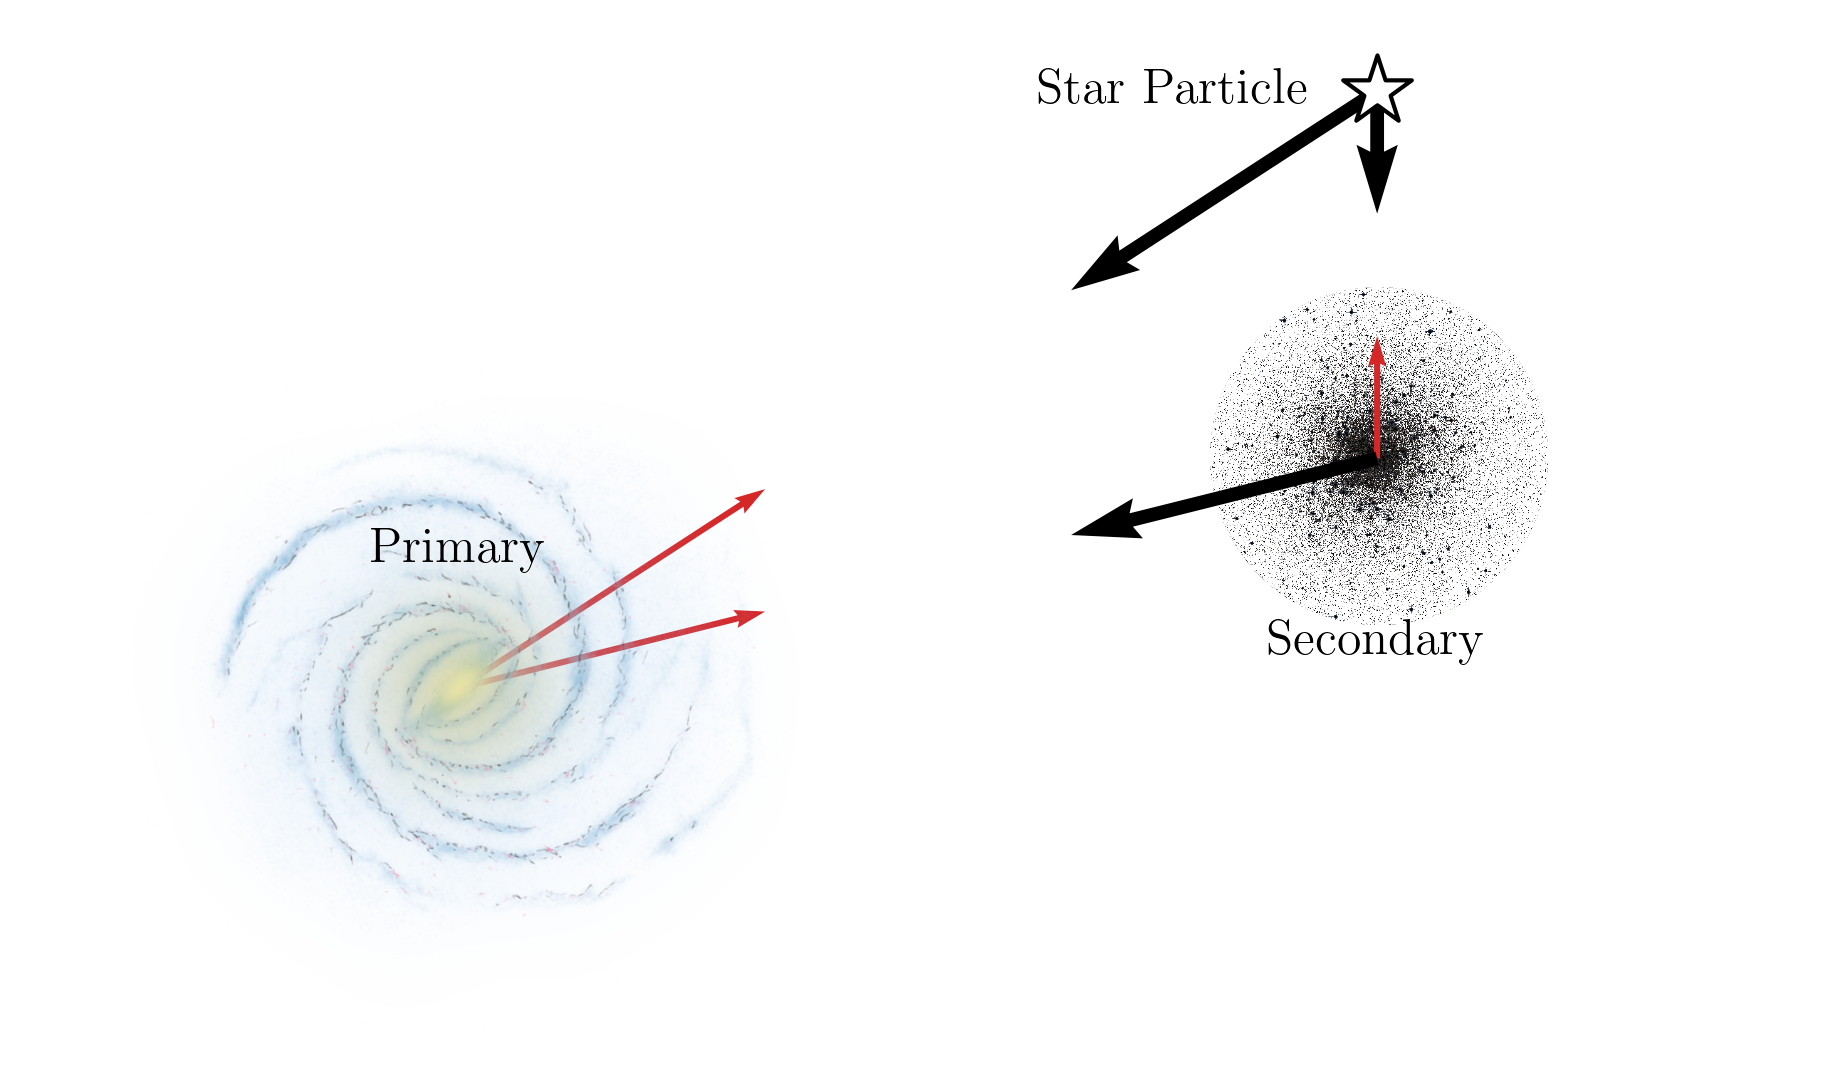
\includegraphics[width=.8\linewidth]{images/restricted_three_body_set_up.png}
        \caption{Schematic illustration of the restricted three-body setup. The system is reduced to three interacting components: the Galaxy (primary), the globular cluster (secondary), and a single star (tertiary). Red vectors indicate forces that are neglected, while the black vectors are those that we model.}
        \label{fig:restricted_three_body_set_up}
    \end{figure}

    This formulation dramatically simplifies the dynamics: the full $N$-body problem is approximated by \(N\) independent realizations of the restricted three-body problem. This reduction allows us to efficiently simulate the formation and evolution of tidal features without incurring the computational cost of tracking all mutual interactions among stars. This approximation has been shown to work very well for certain stellar streams and this thesis is not the first time such methods have been employed. For instance, consider the work of \citet{2012A&A...546L...7M}, who modeled the evolution of the Palomar~5's stellar stream with both an $N$-body code as well as the restricted~three body problem. The differences between the two models for reproducing many characteristics of the stream are minimal. 

    In the remainder of this section, I present the theoretical framework underlying the simulations. At their core, the simulations involve solving \(N\) sets of six coupled ordinary differential equations—one set for each star particle. Section~\ref{subsec:myEquationsOfMotion} introduces the equations of motion. Section~\ref{subsec:gravfield} describes the gravitational field used to compute the forces acting on the particles. Finally, Section~\ref{subsec:initialconditions} details the procedure used to generate initial conditions that faithfully represent a globular cluster.


    
    \subsection{Equations of Motion} \label{subsec:myEquationsOfMotion}

        In galactic dynamics, we can well describe the motion of stars through Poisson's equation, which extends Newton's law of gravity from point masses to smooth density distributions: 
        \begin{equation} \label{eq:poissonsequation}
            \nabla^2 \Phi = 4\pi G \rho,
        \end{equation}
        where $\rho$ is the mass density and $\Phi$ is the gravitational potential. We use Newtonian mechanics throughout this work because $\Phi << c^2$ in all relevant regimes, meaning General Relativity is not required \citep[see Appendix C of][]{bovy_inprep}. Poisson's equation assumes Newton's postulate that gravitational forces act instantaneously and that masses attract each other along the line connecting them. \footnote{Galaxies span millions of light-years, so how can Newton's assumption of instantaneous gravity be valid, given that gravitational waves travel at the speed of light? As shown by \citet{2000PhLA..267...81C}, this is well understood in General Relativity: the gravitational field encodes not only the position but also the motion of massive bodies. This ensures that the resulting spacetime curvature produces a force equivalent to attraction toward the body's instantaneous position, rather than where it was when the gravitational influence was emitted.}

        Instead of writing down the gravitational forces through Newton's second law, I will write down Hamilton's equations derived from the variational principle of Lagrangian mechanics. The full interacting system includes the kinetic energy of the globular cluster and the star particle, as well as three gravitational potential energy terms: the cluster-galaxy interaction, the particle-galaxy interaction, and the particle-cluster interaction:
        \begin{equation}
            \mathcal{L} = \frac{1}{2} M_{\rm gc} \dot{\mathbf{R}}_{\rm gc}^2 
                        + \frac{1}{2} m \dot{\mathbf{r}}^2 
                        - M_{\rm gc} \Phi_{\rm gal}(\mathbf{R}_{\rm gc}) 
                        - m \Phi_{\rm gal}(\mathbf{r}) 
                        - m \Phi_{\rm gc}(\mathbf{r} - \mathbf{R}_{\rm gc}).
        \end{equation}  
        \textbf{annotate the equations}. We decouple the equations of motion of the globular cluster and the star. The justification for this approximation is evident when we normalize the Lagrangian by the cluster mass, \( M_{\rm gc} \). This yields:

        \begin{equation}
            \frac{\mathcal{L}}{M_{\rm gc}} = \frac{1}{2} \dot{\mathbf{R}}_{\rm gc}^2 
                                        - \Phi_{\rm gal}(\mathbf{R}_{\rm gc}) 
                                        + \underbrace{\frac{m}{M_{\rm gc}} \left[ \frac{1}{2} \dot{\mathbf{r}}^2 
                                        - \Phi_{\rm gal}(\mathbf{r}) 
                                        - \Phi_{\rm gc}(\mathbf{r} - \mathbf{R}_{\rm gc}) \right]}_{\text{negligible correction to GC's motion}}
        \end{equation}

        In the limit where \( m << M_{\rm gc} \), the terms in brackets become negligible, and the star's motion has no influence on the cluster. The Lagrangian for the cluster's orbit thus becomes:

        \begin{equation}
            \frac{\mathcal{L}_{\mathrm{gc}}}{M_{\mathrm{gc}}} = \frac{1}{2} \dot{\mathbf{R}}_{\rm gc}^2 
                                - \Phi_{\rm gal}(\mathbf{R}_{\rm gc})
        \end{equation}

        Switching to the star's perspective, we normalize the Lagrangian by the particle mass \( m \), obtaining:

        \begin{equation}
            \frac{\mathcal{L}_{\rm star}}{m} = \frac{1}{2} \dot{\mathbf{r}}^2 
                                - \Phi_{\rm gal}(\mathbf{r}) 
                                - \Phi_{\rm gc}(\mathbf{r} - \mathbf{R}_{\rm gc}(t))
        \end{equation}

        Here, the cluster's influence on the particle is retained through its time-dependent position \( \mathbf{R}_{\rm gc}(t) \). This influence becomes important when the gravitational forces from the cluster and the galaxy on the particle are comparable. For a quick estimate, we treat both the galaxy and the cluster as point masses. The two forces become comparable when the particle is sufficiently close to the cluster, which occurs when: $|\mathbf{r} - \mathbf{R}_\mathrm{GC}| < \sqrt{\frac{M_{\mathrm{gc}}}{M_{\mathrm{ gal}}}} |\mathbf{r}|.$ In other words, the cluster's gravitational field dominates over the galaxy's on sufficiently small scales around the cluster — as expected. For a quick sanity check: a typical globular cluster may have a mass of \(10^5\, M_\odot\), while the galaxy may be around \(10^{11}\, M_\odot\). If the cluster is a few kiloparsecs from the galactic center, then the cluster's influence dominates within a region of order a few parsecs — which checks out. A better limit is the tidal radius and is presented in the next section.

        Next, working in the Hamiltonian formalism often provides deeper insight into the physics of the system. Additionally, Hamiltonian mechanics reduces the equations of motion to a set of \(2N\) first-order differential equations, rather than \(N\) second-order ones, which is more convenient for computational integration.

        The Hamiltonian can then be obtained via a Legendre transform: \(\mathcal{H} = \sum p_i \dot{q}_i - \mathcal{L},\) where $q$ is a generic position coordinate, $p$ is its conjugate momentum, while $i$ indicates the coordinate of interest. If we use the \textit{specific} Lagrangian—normalized by the mass of the body of interest—then, in Cartesian coordinates, the conjugate momenta reduce to the velocities: $p_i=\frac{\partial \mathcal{L}}{\partial q} \rightarrow p_i = v_i$. Another useful result comes from Noether's theorem: if a coordinate does not explicitly appear in the Lagrangian, its conjugate momentum is conserved. All galactic potentials considered in our simulation are axis-symmetric meaning they have cylindrical symmetry (see next section). Since the Lagrangian does not depend on the azimuthal angle \( \theta \) in the \(x\text{-}y\) plane for the cluster's motion, the conservation of the \(z\)-component of angular momentum is conserved: $p_\theta = L_z = \frac{\partial \mathcal{L}}{\partial \dot{\theta}} = R^2 \dot{\theta} = \mathrm{constant.}$

        This conservation generally does not hold for star particles within the globular cluster, as their dynamics are significantly influenced by the cluster's gravitational potential. However, once a star-particle escapes the cluster the conservation of the z-component of the angular momentum is recovered in the regime where their motion becomes dominated by the galaxy's potential. 

        Hamilton's equations thus provide the time evolution of the momenta and the positions. In cartesian coordaintes, the equations of motion for the cluster are: 

        \begin{align}\label{eq:equations_of_motion_cluster}
            \dot{p}_{\mathrm{gc},x} &= -\frac{\partial \Phi_\mathrm{gal}\left(\mathbf{R}_{\mathrm{gc}}\right)}{\partial x} \\
            \dot{p}_{\mathrm{gc},y} &= -\frac{\partial \Phi_\mathrm{gal}\left(\mathbf{R}_{\mathrm{gc}}\right)}{\partial y} \\
            \dot{p}_{\mathrm{gc},z} &= -\frac{\partial \Phi_\mathrm{gal}\left(\mathbf{R}_{\mathrm{gc}}\right)}{\partial z} \\
            \dot{x}_{\mathrm{gc}} &= p_{\mathrm{gc},x} \\
            \dot{y}_{\mathrm{gc}} &= p_{\mathrm{gc},y} \\
            \dot{z}_{\mathrm{gc}} &= p_{\mathrm{gc},z}.
        \end{align}
        For the star particle, the equations of motion become: 
        \begin{align}\label{eq:equations_of_motion_stream}
            \dot{p}_{x} &= -\frac{\partial \Phi_\mathrm{gal}\left(\mathbf{r}\right)}{\partial x} - \frac{\partial \Phi_\mathrm{gc}\left(\mathbf{r} - \mathbf{R}_{\mathrm{gc}}(t)\right)}{\partial x}\\
            \dot{p}_{y} &= -\frac{\partial \Phi_\mathrm{gal}\left(\mathbf{r}\right)}{\partial y} - \frac{\partial \Phi_\mathrm{gc}\left(\mathbf{r} - \mathbf{R}_{\mathrm{gc}}(t)\right)}{\partial y}\\
            \dot{p}_{z} &= -\frac{\partial \Phi_\mathrm{gal}\left(\mathbf{r}\right)}{\partial z} - \frac{\partial \Phi_\mathrm{gc}\left(\mathbf{r} - \mathbf{R}_{\mathrm{gc}}(t)\right)}{\partial z}\\
            \dot{x} &= p_x \\
            \dot{y} &= p_y \\
            \dot{z} &= p_z,
        \end{align} 
        where $\mathbf{r} = \left(x,y,z\right)$. Note that equation~\ref{eq:equations_of_motion_stream} describes the motion of a single particle. In general, if we use 100,000 particles, the motion of each is described with this same equation, but has different initial conditions. 
        
        In Chapter~5, we modify Equation~\ref{eq:equations_of_motion_cluster} to compute the $N$~body forces between all the clusters. While we created these equations to avoid $N$-body computations, it is not too computationally expensive to implement this for the cluster's themselves since we only have about 160 clusters. These equations are modified by:  
        \begin{align}\label{eq:equations_of_motion_cluster_n_body}
            \dot{p}_{x,i} = - \frac{\partial \Phi_\mathrm{gal}}{\partial x} - \sum_{j\neq i}^N \left[\frac{\partial \Phi_\mathrm{gc}\left(\mathbf{R}_i-\mathbf{R}_j|M_j,b_j\right)}{\partial x}\right], \\ 
            \dot{p}_{y,i} = - \frac{\partial \Phi_\mathrm{gal}}{\partial y} - \sum_{j\neq i}^N \left[\frac{\partial \Phi_\mathrm{gc}\left(\mathbf{R}_i-\mathbf{R}_j|M_j,b_j\right)}{\partial y}\right], \\ 
            \dot{p}_{z,i} = - \frac{\partial \Phi_\mathrm{gal}}{\partial z} - \sum_{j\neq i}^N \left[\frac{\partial \Phi_\mathrm{gc}\left(\mathbf{R}_i-\mathbf{R}_j|M_j,b_j\right)}{\partial z}\right],
        \end{align}
        where $i$ is the index of a target cluster and $j$ iterates over the others. Note that in $\Phi_{\mathrm{gc}}$, I explicitly write $M_j,b_j$ to indicate the mass and scale length of the $j^{\mathrm{th}}$ cluster. Each cluster has it's own scale-length, which were computed from the half-mass radii reported in \citet{2018MNRAS.478.1520B}. Since the scale lengths differ from each cluster, we violate Newton's third law: $\dot{p}_{ij} \neq - \dot{p}_{ji}$. However, this is a minor consequence. Since I model each cluster as a Plummer sphere (as explained in the next section), at distances much greater than the scale radius, the functional form is the same as a point mass. 

        Lastly, in terms of the stream generation for Chapter~5, equation~\ref{eq:equations_of_motion_stream} are also modified to include the force from all the clusters, instead of just the host cluster. This becomes: 
        \begin{align}
            \dot{p}_{x} &= -\frac{\partial \Phi_\mathrm{gal}\left(\mathbf{r}\right)}{\partial x} - \sum_i^N \frac{\partial \Phi_\mathrm{gc}\left(\mathbf{r} - \mathbf{R}_i(t)\right)}{\partial x}\\
            \dot{p}_{y} &= -\frac{\partial \Phi_\mathrm{gal}\left(\mathbf{r}\right)}{\partial y} - \sum_i^N \frac{\partial \Phi_\mathrm{gc}\left(\mathbf{r} - \mathbf{R}_i(t)\right)}{\partial y}\\
            \dot{p}_{z} &= -\frac{\partial \Phi_\mathrm{gal}\left(\mathbf{r}\right)}{\partial z} - \sum_i^N \frac{\partial \Phi_\mathrm{gc}\left(\mathbf{r} - \mathbf{R}_i(t)\right)}{\partial z}
        \end{align}

        The equations of motion listed above are what are used for the experiments presented in Chapters~4~\&~5, respectively. The first two sets of equations are those used when generating the streams through the resectried three body problem, while the second set generate the streams in a Milky Way where other globular clusters fly around and can perturb a given stream. The next two subsections introduce the various forms that $\Phi$ can take, followed by the generation of the initial conditions. 


    \subsection{The Gravitational Field} \label{subsec:gravfield}
        Determining the gravitational field of the Milky Way remains an open and complex problem. From our location within the Galaxy, it is difficult to obtain a global perspective. Since the advent of extragalactic astronomy and early classification efforts such as those by \citet{1926ApJ....64..321H}, we have begun to ask what the total structure of our own Galaxy is. Before providing a robust estimate for the global mass distribution, some simpler questions were addressed. For example, \citet{1927BAN.....4...91O} studied the motion of stars in the local solar neighborhood and showed that the Galaxy not only has net rotation, but also differential rotation—as opposed to solid-body rotation.

        The field has come a long way since then, and today we possess a number of viable models for the Galactic gravitational potential. Much of this progress owes to the fact that Poisson's equation is linear:
        \begin{equation}\label{eq:linear_poisson}
            \nabla^2 \left(a_0\Phi_0 + a_1\Phi_1 \right) = a_0 \nabla^2 \Phi_0 + a_1 \nabla^2 \Phi_1 = 4\pi G \left(a_0\rho_0 +a_1\rho_1\right),
        \end{equation}
        which allows us to treat the Galaxy as a superposition of separate components, each described by its own potential-density pair. This decomposition enables the construction of composite models from a collection of structural elements that are also commonly observed in external galaxies. The Galaxy Zoo project \citep{2008MNRAS.389.1179L}, for instance, has shown that many galaxies—including our own—share similar morphologies, justifying this modular approach. Typical components of disc like galaxies, the Milky Way included, are:
        \begin{itemize}
            \item A stellar disk,
            \item A gaseous disk,
            \item A dark matter halo,
            \item A stellar halo,
            \item A bulge,
            \item A galactic bar,
            \item Spiral arms.
        \end{itemize}

        In addition, smaller-scale structures such as globular clusters, giant molecular clouds, and open clusters can locally perturb the field. Even external sources, such as the Large and Small Magellanic Clouds, play a role by inducing measurable tidal effects on the Galaxy \citep{2022ApJ...939....2A}.

        Despite this framework, modeling remains difficult because the structural components are not isolated. As emphasized by \citet{2016ARA&A..54..529B}, the components co-evolve within a shared potential, meaning that even those formed separately eventually become dynamically mixed. This interdependence implies that the potential cannot be cleanly partitioned into independent contributions, and even with a complete dataset, degeneracies would persist. Their review illustrates this point by listing 37 parameter groups required to characterize the Galaxy—including the local standard of rest, Galactic reference frame, and the geometric and density properties of various components—underscoring the system's complexity.

        The challenge is compounded by limitations in the available data. The Gaia mission has delivered the most comprehensive survey of the Galaxy to date \citep{2023A&A...674A...1G}, providing photometric and astrometric data for over two billion stars and radial velocities for tens of millions \citep{2018A&A...616A..11G}. However, this still represents only a small fraction of the total stellar population. The stellar mass of the Milky Way is estimated to be approximately $6\times10^{10} \mathrm{M}_\odot$ \citep{2015ApJ...806...96L}, corresponding to roughly one hundred billion stars \citep[see also][]{2017MNRAS.465...76M}. Thus, Gaia provides 5D phase-space information for only about 1-2\% of all stars, and full 6D information for just a fraction of a percent.

        Moreover, the data suffer from unavoidable selection effects. As illustrated in Fig.~\ref{fig:gaia_selection_function}, which shows the spatial distribution of stars with spectroscopic observations from Gaia DR3, the bulk of high-quality measurements are clustered near the Sun. This is a natural consequence of the inverse-square law for luminosity, and it implies that any model of the Galactic potential must account for these biases. Such limitations are likely to remain significant for the foreseeable future.

        \begin{figure}
            \includegraphics[width=\linewidth]{images/recio-blanco-2023-fig5}
            \caption{The Gaia spatial selection function for spectroscopic observations. Figure 5 from \citet{2023A&A...674A..38G}.}
            \label{fig:gaia_selection_function}
        \end{figure}

        In summary, while we now possess sophisticated models and rich datasets, constructing a comprehensive and precise model of the Milky Way's gravitational field is still inherently difficult—constrained both by observational incompleteness and the physical complexity of a system in which all components are tightly coupled. Given these challenges, the construction of a Galactic model depends on the scientific question being asked.

        Consider \texttt{TRILEGAL} \citep{2005A&A...436..895G}. This model aims to answer the question: if I observe the sky from a given location with a given instrument, what do I expect to see? The focus of these models are stellar populations. Dynamics—such as orbits or gravitational forces—are secondary and not included in the construction. The primary goal is to reproduce observed star counts and understand the underlying stellar populations. Such models are designed to simulate the sky as it would appear to missions like Hipparcos \citep{1997A&A...323L..49P}, 2MASS \citep{2006AJ....131.1163S}, and SDSS \citep{2000AJ....120.1579Y}.

        Some models attempt to address both stellar populations and dynamics. For example, the Besançon model aims to construct a dynamically self-consistent model of the Milky Way that reproduces observables such as the rotation curve, as well as the spatial and chemical distributions of stars. The model originated with \citet{2003A&A...409..523R}, who constrained it primarily using Hipparcos data. Their initial decomposition included a thin disk, a thick disk, a stellar halo, and a bulge, with each component assigned its own star formation rate and initial mass function. The model has been continuously refined; for instance, \citet{2022A&A...667A..98R} incorporated Gaia DR3 kinematics to further constrain it. As noted by \citet{2025AJ....169..317K}, who recently introduced the open-source Python package \texttt{SYNTHPOP} for simulating on-sky photometry, the success of TRILEGAL and the Besançon model lies in their openness: they are publicly available and have web interfaces for widespread use. These tools are particularly valuable for creating mock surveys of the sky.

        A different approach is taken by \citet{2024MNRAS.527.1915B}, building on \citet{2023MNRAS.520.1832B}, who constructed a dynamical model of the Milky Way in which the distribution function depends on orbital actions—quantities that are conserved along orbits in a steady-state potential. In axisymmetric potentials, the actions are $J_r$, $J_\phi$, and $J_z$, and represent how much motion an orbit has in the radial, azimuthal, and vertical directions, respectively. The moments of the distribution function yield observable quantities such as stellar surface densities, volume densities, and velocity dispersions. In addition to dynamical consistency, the model includes the chemical properties of stars, specifically metallicity ([Fe/H]) and $\alpha$-element abundances. The model is constrained using Gaia DR3 data \citep{2023A&A...674A...1G}, particularly stars with full phase-space information, as well as APOGEE DR17 \citep{2017AJ....154...94M}. Their model involves over 40 parameters to describe the distributions of stars and metallicities throughout the Milky Way.

        Then, there are many models of the Milky Way that are primarily dynamically motivated, with stellar populations treated as secondary \citep{1991RMxAA..22..255A,2015ApJS..216...29B,2017MNRAS.465...76M,2017A&A...598A..66P,2024ApJ...967...89I}. Despite the variety, their construction generally follows the same template: the authors must choose which dataset to use, which tracer populations to include, and the parametric form of the Milky Way potential. Often, fitting all model parameters is infeasible, whether due to lack of data, high computational cost, or non-converging likelihoods.

        All of the above models assume axisymmetry, which is already a limitation. This makes it difficult to model the dynamics in the inner Galaxy (within $2~\mathrm{kpc}$) or for the most bound stars — though these are not necessary for modeling orbits outside that region. Both \citet{2017MNRAS.465...76M} and \citet{2024MNRAS.527.1915B} fix the parameters describing the gas in the Galactic disk and only fit those related to the stellar and dark matter distributions. \citet{2017MNRAS.465...76M} specifically constructed their model to support orbit calculations for stars in anticipation of Gaia data releases. They aimed to improve upon their earlier model \citep{2011MNRAS.414.2446M}, motivated by (1) a tripling of the maser population used to trace disk kinematics, and (2) the realization that omitting a gaseous disk in their earlier work had led to underestimating the forces in the solar vicinity.

        Many of the models described above rely on fitting data using kinematic information — comparing the model's predictions for velocity dispersion to observations of large samples of stars. This is because direct astrometric measurements of stellar accelerations are still in their infancy. Measuring changes in angular position through parallax is so challenging that stars were long referred to as \textit{fixed stars} \citep{1981unht.book.....K}. Precise, year-over-year positional measurements are required to observe motion on the celestial sphere — precisely what Gaia does. \textbf{Whose uncertainties are lower: proper motions or radial velocities? Is it possible to measure accelerations using radial velocities?}

        That said, accelerations have been measured in some cases. \citet{2018ApJS..239...31B,2021ApJS..254...42B} created a cross-catalog between Hipparcos and Gaia DR2 \citep{2018A&A...616A...1G} and later EDR3. This provided a baseline of over 25 years, long enough to detect accelerations for some stars. However, the Hipparcos catalog only contains around 100,000 stars, and the typical acceleration of a field star in the Galaxy is extremely small. Consequently, the cross-matched catalog is currently being used to study stars with unusually high accelerations — typically in binary systems or with massive planets \citep{2023MNRAS.521.5232W,2025AJ....170...52G} — rather than to measure Galactic accelerations.

        As stated in the motivation for undertaking this thesis, stellar streams are particularly to this recovering information about the galactic gravitational field. The stars within a stream are on similar orbits (but shifted in phase), and their orientation and curvtature encodes detailed information about the Galactic gravitational field. \citet{2024ApJ...967...89I} is the first study to use stellar streams to directly fit a gravitational potential model of the Milky Way. Even in that case, \citet{2024ApJ...967...89I} fixed some of the model parameters, adopting the same bulge model as \citet{2017MNRAS.465...76M}.

        In this thesis, we use the model of \citet{2017A&A...598A..66P}, which builds upon \citet{1991RMxAA..22..255A}. This model was developed within our research group and made available at the start of the project. It was designed to fit observational data similar to those used in \citet{2015ApJS..216...29B}, including the galactic rotation curve and local stellar kinematics. \citet{2017A&A...598A..66P} provides two versions of the model — one with a bulge and one without. Below, we describe the second version, which we used in both Chapter~4 and Chapter~5.

        The second version of \citet{2017A&A...598A..66P} models the Galaxy with a halo, and thin and thick disks. One advantage of this model is that the gravitational potential of each component is analytic. For example, the Miyamoto-Nagai potential \citep{1975PASJ...27..533M} is fully analytic and given by:
        \begin{equation}
            \Phi(R, z \mid M, a, b) = -\frac{G M}{\sqrt{R^2 + \left(a + \sqrt{z^2 + b^2}\right)^2}},
        \end{equation}
        where $M$ is the total mass of the disk, $a$ is the radial scale length, and $b$ is the vertical scale height. This form smoothly interpolates between a flattened disk and a spherical distribution, depending on the values of $a$ and $b$. \citet{2017MNRAS.465...76M} also used this form for their disk model.

        However, it is worth noting that real galaxies are observed to have exponentially decaying disks:
        \begin{equation}
            \rho(R,z) = \rho_0 \mathrm{exp}\left(-\frac{R}{R_d}-\frac{|z|}{z_d}\right),
        \end{equation}
        where $\rho$ is the mass density, $R$ is the cylindrical radius, $z$ the vertical height, and the model has three parameters: a characteristic density $\rho_0$, scale radius $R_d$, and scale height $z_d$. A drawback of this model is that it cannot be integrated analytically to obtain the potential, since the $R$ and $z$ coordinates are not separable. Often, basis function expansions are needed to approximate the potential and compute forces. \citet{2017MNRAS.465...76M} and \citet{2024ApJ...967...89I} both adopted this model for their Galactic disks.

        Regarding the halo, \citet{2017A&A...598A..66P} do not separate the dark matter and stellar halo components. Instead, they use a single halo model to represent the total gravitational contribution from both. This model is inherited from \citet{1991RMxAA..22..255A}, originally proposed in \citet{1986RMxAA..13..137A}. It is designed so that beyond a certain scale radius, the enclosed mass grows linearly with distance, leading to the desirable feature of a flat rotation curve:
        \begin{equation} 
            M_{\mathrm{enc}}(r|M_0,\gamma,r_0,r_c) = M_0
            \begin{cases}
             \frac{\left(r/r_0\right)^\gamma}{1 + \left(r/r_0\right)^{\gamma - 1}} & r<r_c,\\
             \frac{\left(r_c/r_0\right)^\gamma}{1 + \left(r_c/r_0\right)^{\gamma - 1}} & r> r_c,\\
            \end{cases} 
            \label{eq:martos_enclosed_mass}
        \end{equation}

        where $M_0$ is a mass scaling parameter (not the total mass), $r_0$ is the characteristic radius, $\gamma$ is the power-law index, and $r_c$ is a cutoff radius beyond which the mass is held constant. Thus, for $r > r_c$, Eq.~\ref{eq:martos_enclosed_mass} yields the total mass. 

        In the outer regime $(r/r_0) >> 1$, the enclosed mass scales as $M(r) \propto r$, producing a flat rotation curve. In the inner regime $(r/r_0) << 1$, the mass grows as a power law, $M(r) \propto r^{\gamma - 1}$, which provides flexibility in shaping the central density slope. Since the unmodified profile leads to an unphysical divergence in total mass, a truncation at $r_c$ is imposed.

        Assuming spherical symmetry, we may use the relation $\nabla \Phi = \frac{G M_{\mathrm{enc}}(r)}{r^2}$. Requiring that the potential vanish at infinity, the corresponding gravitational potential can be obtained by integrating:
        \begin{equation}
            \Phi(r|M_0,\gamma,r_0,r_c) = 
            \begin{cases}
                \frac{GM_0}{r_0\left(\gamma-1\right)}\ln\left|\frac{1+(r/r_0)^{\gamma-1}}{1+(r_c/r_0)^{\gamma-1}}\right| -\frac{GM_t}{r_c}, & r<r_c\\
                -\frac{GM_t}{r} & r>r_c.
            \end{cases}
        \end{equation}
        where $M_t$ denotes the total mass, $M_{\mathrm{enc}}(r_c)$.

        In general, a good halo model should reproduce the observed flat rotation curve at large radii. Another class of models that achieves this are the double power-law profiles:
        \begin{equation}
            \rho(r \mid \alpha, \beta, r_s) = \rho_0 \left( \frac{r}{r_s} \right)^{-\alpha} \left(1 + \frac{r}{r_s} \right)^{\alpha - \beta},
        \end{equation}
        where $r_s$ is a scale radius, $\alpha$ controls the inner slope, and $\beta$ the outer slope. Common choices include the NFW profile ($\alpha = 1$, $\beta = 3$) and the Hernquist profile ($\alpha = 1$, $\beta = 4$). These families of models were implemented in the works of \citet{2015ApJS..216...29B, 2017MNRAS.465...76M} to describe the dark matter halo.

        The second Galactic potential model presented in \citet{2017A&A...598A..66P} consists of two Miyamoto-Nagai disks plus the Martos halo and is shown in Fig.~\ref{fig:figure_pouliasis2017pii_potential}. More visualizations of this potential can be found in their work.
        \begin{figure}
            \centering
            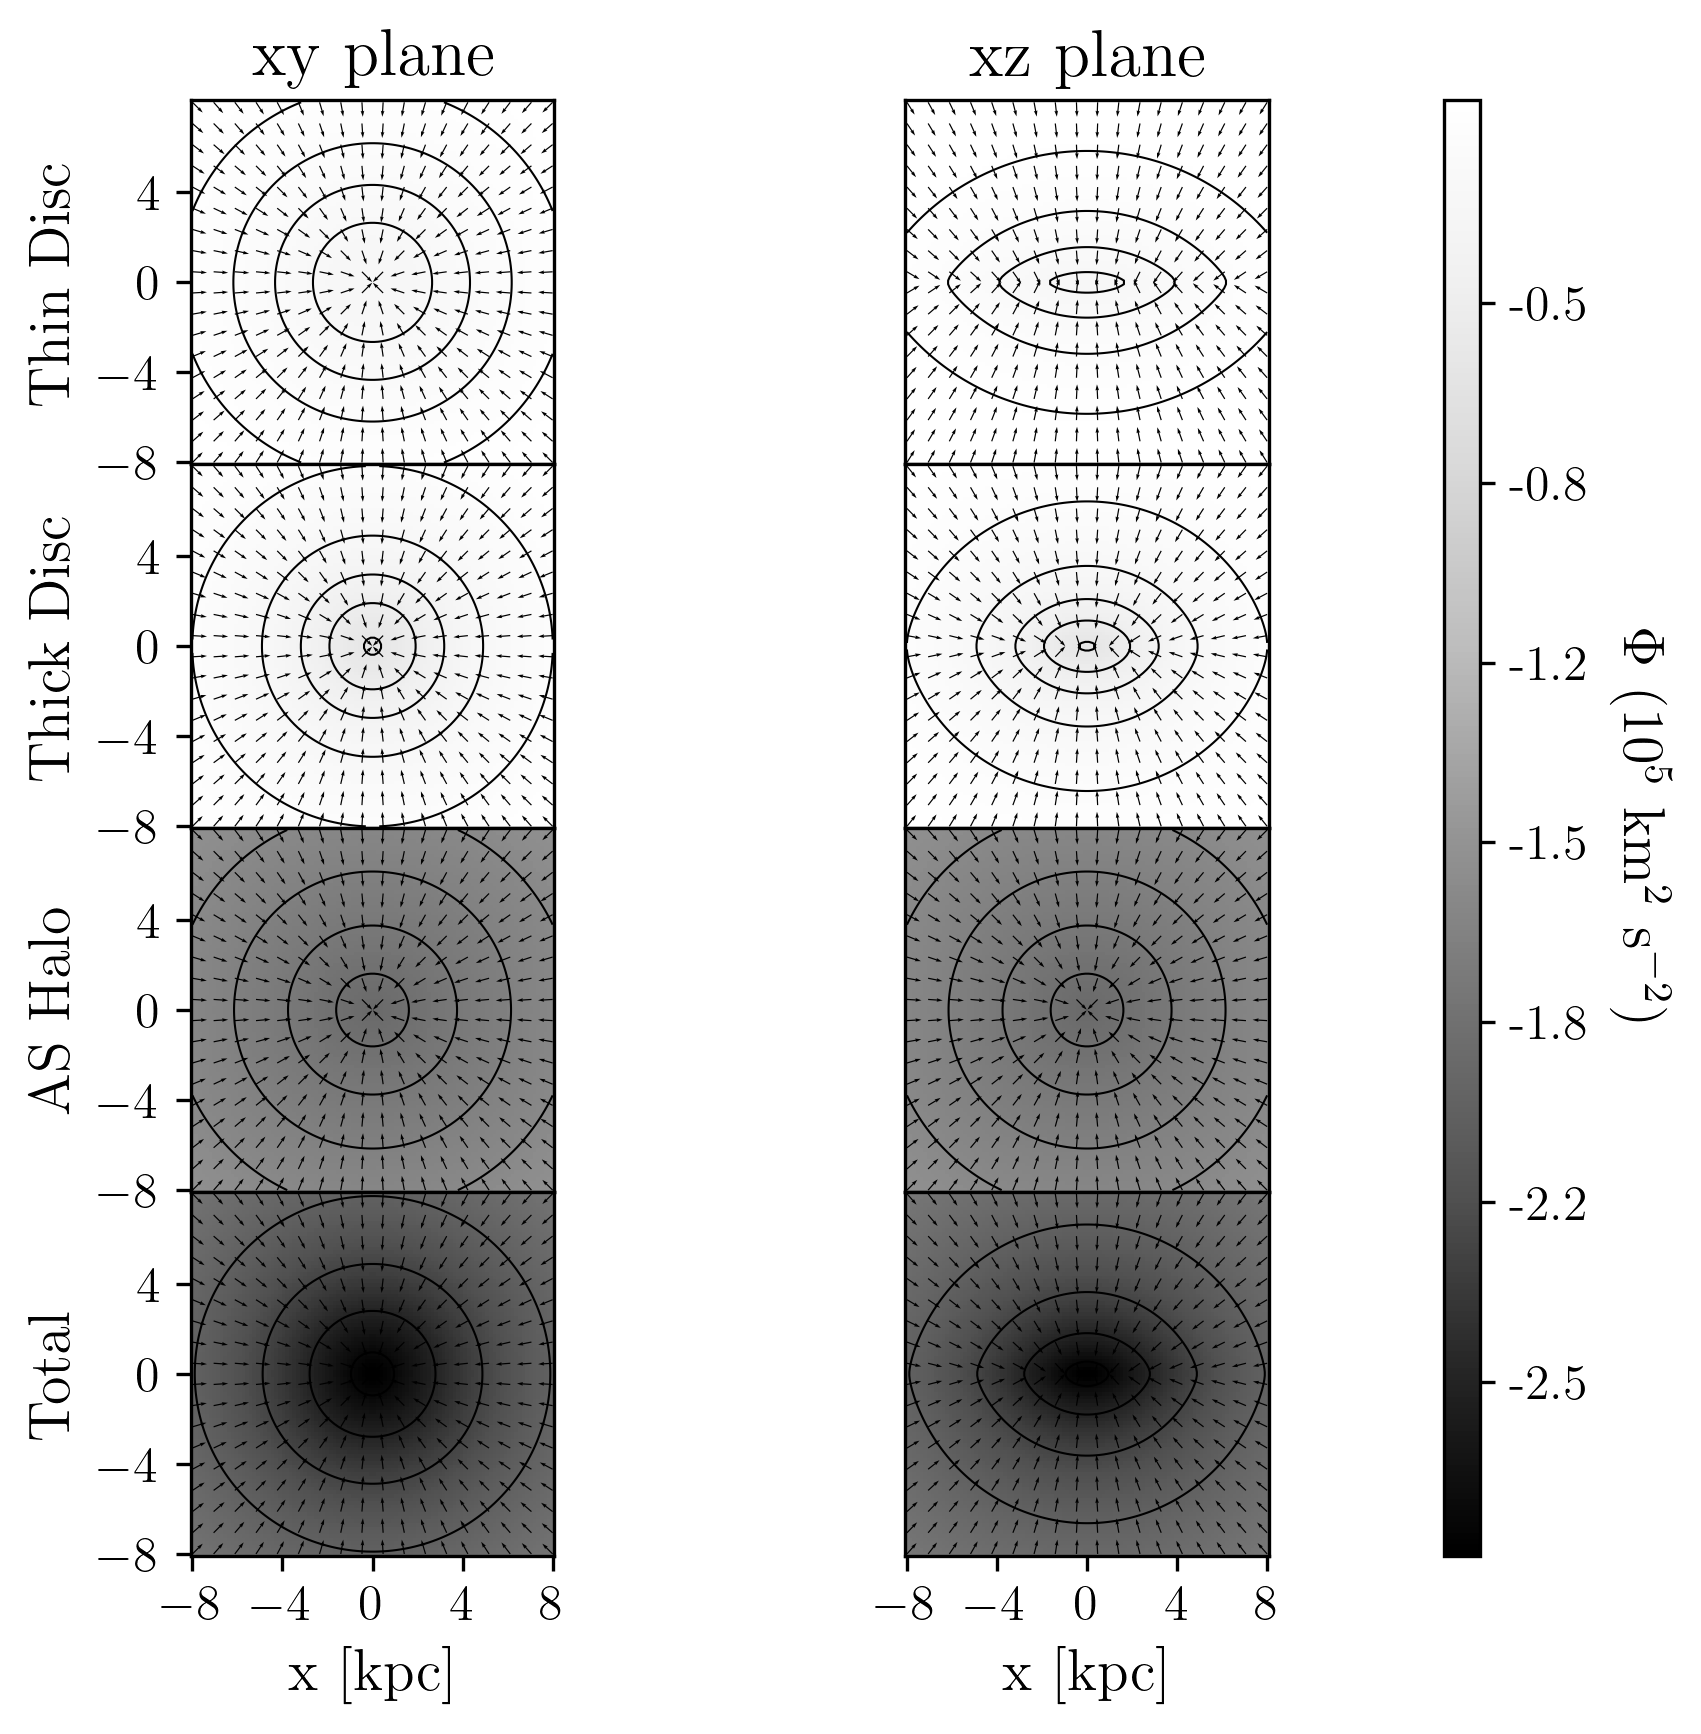
\includegraphics[width=\linewidth]{images/figure_pouliasis2017pii_potential_-8_8.png}
            \caption{Individual components of the second Galactic potential model from \citet{2017A&A...598A..66P}. The vector field illustrates the normalized gravitational force at each position, corresponding to $\vec{g} = -\nabla\Phi$. Equipotential contour lines are overlaid to guide the eye.}
            \label{fig:figure_pouliasis2017pii_potential}
        \end{figure}        
        How important is the choice of potential model when modeling the orbits of globular clusters? It depends on the specific cluster. Take, for instance, Fig.~\ref{fig:vasiliev_2021_EDR3_GCS_FIG_10}. The position and spread of some clusters are virtually identical between different models—for example, NGC~288. This suggests that the observational uncertainties in the kinematic data are larger than the discrepancies introduced by the choice of potential. However, for other clusters, the model choice has a much greater impact. A notable case is Pyxis, where the inferred orbits differ significantly depending on the potential. This effect is more pronounced for clusters located farther from the Galactic center, where the models diverge more strongly.

        \begin{figure}
            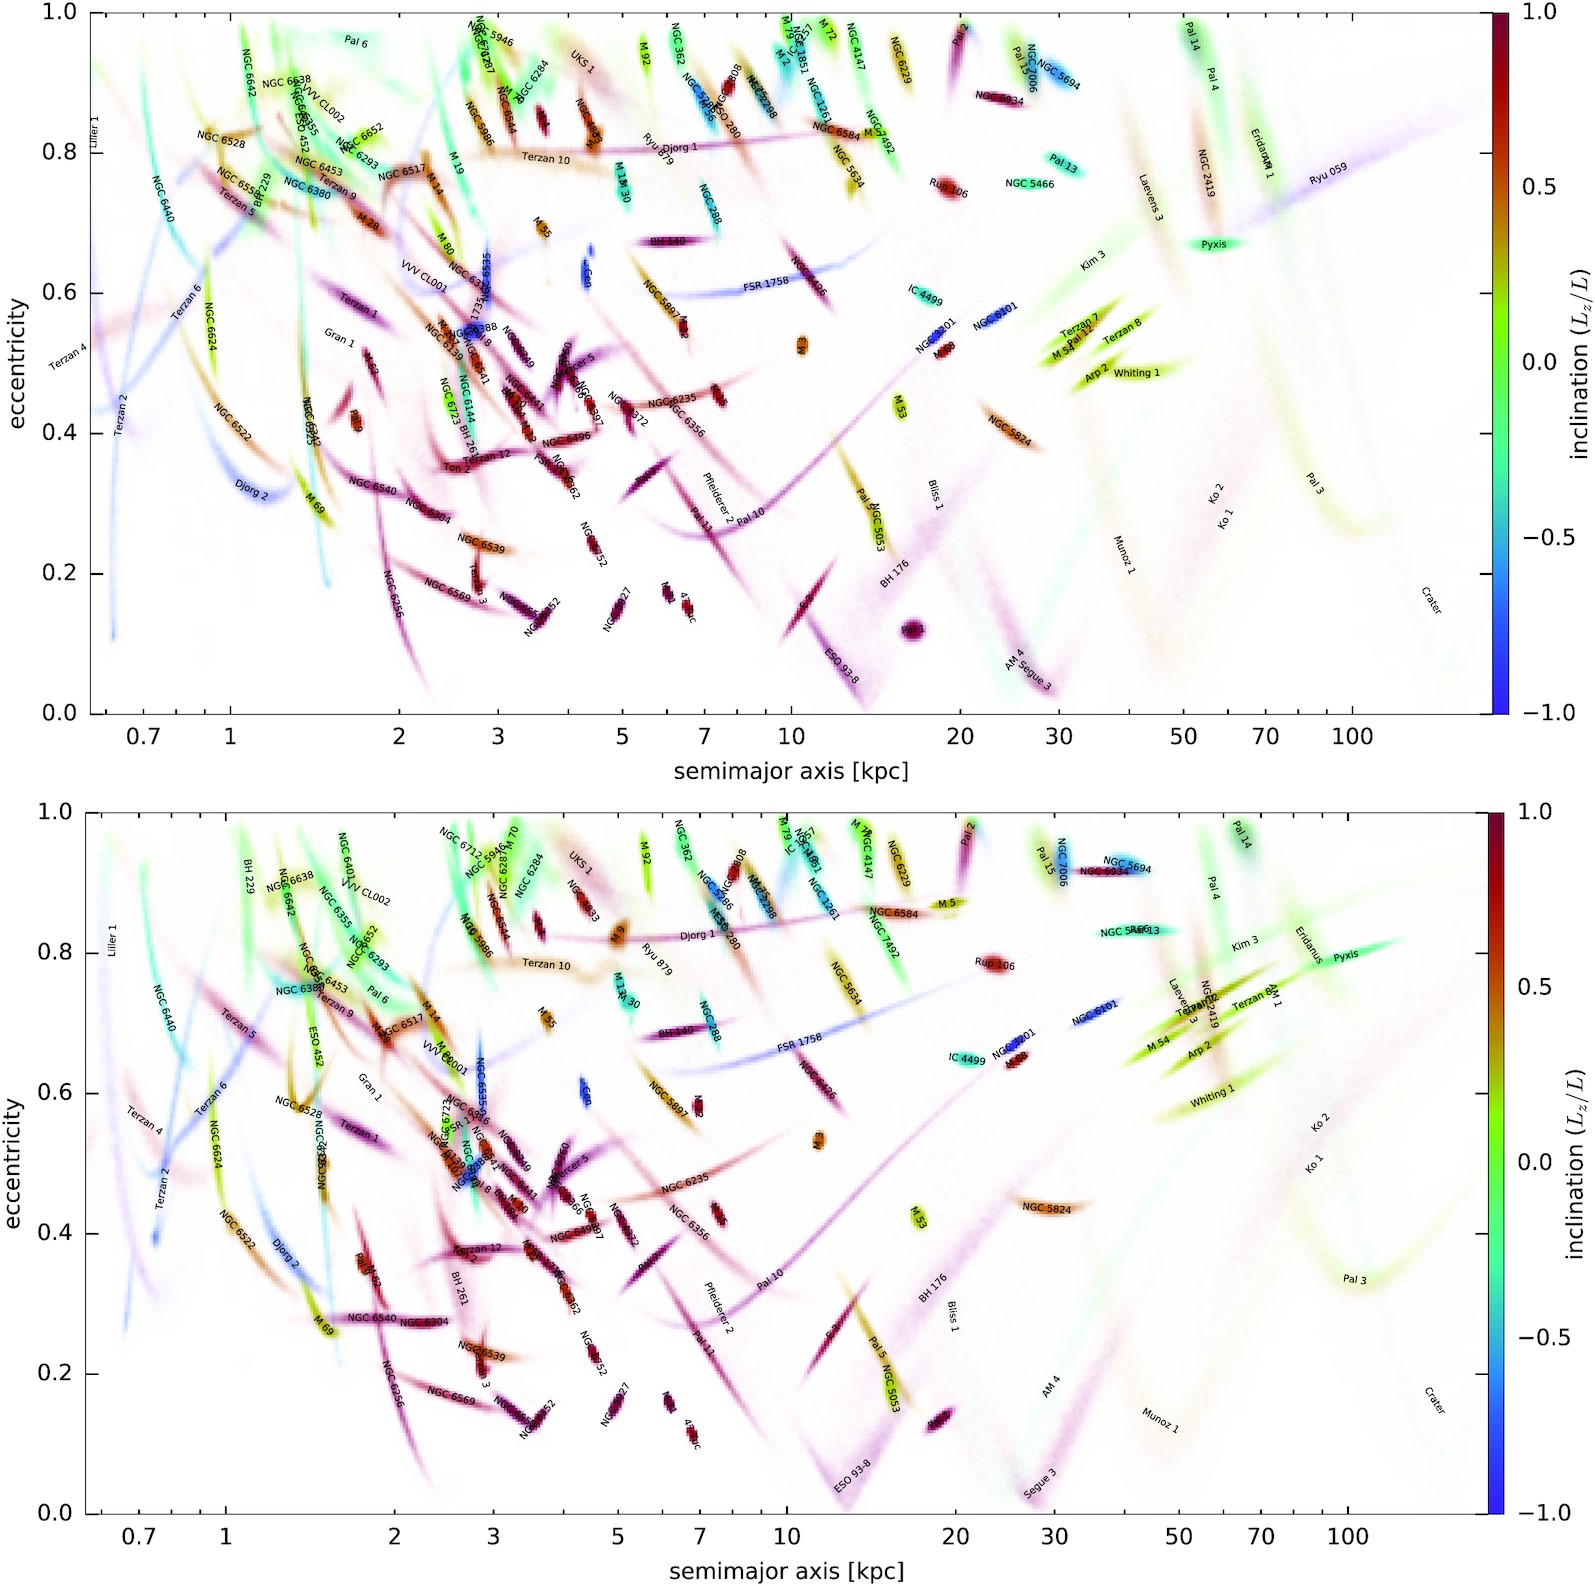
\includegraphics[width=\linewidth]{images/vasiliev_2021_EDR3_GCS_FIG_10.jpeg}
            \caption{Distribution of eccentricities, inclinations, and semi-major axes for the globular cluster population, based on Gaia EDR3 kinematics. Each point corresponds to a single realization of a globular cluster orbit, given its observational uncertainties. The top panel shows orbits computed using the potential from \citet{2017MNRAS.465...76M}, while the bottom panel uses the model from \citet{2015ApJS..216...29B}. (Credit: Fig.~10 from \citet{2021MNRAS.505.5978V})}
            \label{fig:vasiliev_2021_EDR3_GCS_FIG_10}
        \end{figure}

        Differences in cluster orbits-or in stellar streams evolved in different potentials-can help constrain the underlying Galactic potential and eventually lead to more accurate models of the Milky Way. This was the motivation behind recent work such as \citet{2024ApJ...967...89I}. However, if the goal is to make robust predictions or extrapolate properties of the halo, it is prudent to explore a variety of Galactic models, especially when no single model is clearly preferred.

        What about the self-gravity of the globular cluster itself? Here we adopt one of the simplest available models: the Plummer sphere \citep{1911MNRAS..71..460P}. This model has two parameters—the total mass and a scale length—and takes the form
        \begin{equation} \label{eq:plummer}
            \Phi(r \mid M, b) = -\frac{G M}{\sqrt{r^2 + b^2}},
        \end{equation}
        where $M$ is the total mass and $b$ is the scale length. In the limit $a \rightarrow 0$, the Miyamoto-Nagai potential reduces to a Plummer sphere. This model has a minimum potential at the center, recovers the potential of a point mass at large distances ($r >> b$), and yields a density profile that decays as $\rho \propto r^{-5}$ at large radii.

    
    \subsection{Generating a Globular Cluster}\label{subsec:initialconditions}

        Now that we have our equations of motion established, and we have an accurate model for computing the gravitational force at each point in the galaxy, what are the initial conditions? First, the initial conditions for the center's of mass of the globular clusters, their mass and size, are taken observationally from \citet{2018MNRAS.478.1520B}. What about the stars within the cluster? 

        We have choosen the potential for each cluster to be a Plummer sphere from Eq.~\ref{eq:plummer}, which meanns that it is more massive in the center and whose density decreases with a power law beyond the characteristic radius. We can use this to obtain a mass profile, and then sample this distribution to obtain initial positions for each particle. 

        Unfortunately, positions alone are not enough, for we must also know the velocities. After sampling the positions, we could do something crude by saying that each star has a velocity vector that could point in any direction with equal probability. This is known as being \textit{isotropic} or equally random. Next, we could say that a star's speed could be anywhere from zero to the escape velocity. While this would work to create a set of plausible initial conditions, it would not be \textit{self-consistent}. 

        In galactic dynamics, a fundamental challenge is the \textit{self-consistency problem}. This involves a loop of three steps:  
        \begin{enumerate}
            \item Given a density distribution and a gravitational potential (linked via Poisson's equation), one samples the positions of stars.  
            \item One then assigns initial velocities and evolves the system forward in time.  
            \item The potential is updated based on the evolved mass distribution.
        \end{enumerate}

        If the system is in equilibrium and self-consistent, then the mass distribution remains stable under its own gravity. That is, the same density that generated the potential continues to persist as the system evolves. For the rest of the section, I will describe in detail how one creates a self consistent system through the Collisionless Boltzmann Equation, and the simplifying assumptions employed in this thesis tackle our specific problem.

        Our starting point is to characterize the system statistically, with a distribution function (DF) over phase-space. That is, what is the probability density of finding a particle at a given position and velocity? This is encoded in the function \( f(\vec{x}, \vec{v}, t) \). If we treat this as a true probability density function that integrates to 1 over all phase space, we are implicitly assuming a closed system: no stars enter, leave, are born, or die.

        Already, by writing \( f(\vec{x}, \vec{v}, t) \), we are assuming that a particle's phase-space position is independent of any other attributes — such as mass. Let us define \( \mathbf{w} = (\vec{x}, \vec{v}) \) as the 6D phase-space coordinate. Then, for a system of \( N \) particles, the full distribution function lives in \(6N\)-dimensional space:  
        \[
        f(\mathbf{w}_1, \dots, \mathbf{w}_N)
        \]  
        This expression represents the joint probability density of finding particle 1 at \( \mathbf{w}_1 \), particle 2 at \( \mathbf{w}_2 \), and so on. In general, this object can be extremely complicated. But we can simplify it with two strong assumptions: that particles are independent and identically distributed (i.i.d.). This leads to:

        \[
        \begin{array}{rl}
        f 
        & \stackrel{\text{(1) $N$-body DF}}{\longrightarrow} 
        f(\mathbf{w}_1, \dots, \mathbf{w}_N) \\[2ex]
        & \stackrel{\text{(2) independence}}{\longrightarrow} 
        \prod_{i=1}^N f^i(\mathbf{w}_i) \\[2ex]
        & \stackrel{\text{(3) identical distribution}}{\longrightarrow} 
        \left[ f(\mathbf{w}) \right]^N
        \end{array}
        \]

        The consequence of this factorization is that the total DF no longer accounts for correlations in other variables — such as mass. Therefore, this model cannot represent mass segregation, multiple stellar populations, or any other effects that differentiate stars. Instead, we describe a single homogeneous population of stars, each drawn independently from the same distribution.

        Because of this, we can focus our attention entirely on the single-particle DF \( f(\mathbf{w}) \), which encodes all the statistical information we need about the system.

        The next key assumption is that particles are uncorrelated not just in identity, but dynamically — they do not scatter off one another. This means the system is \textit{collisionless}. The DF then evolves under the Collisionless Boltzmann Equation:

        \begin{equation}
        \frac{Df}{Dt} = \frac{\partial f}{\partial t} + \dot{\mathbf{x}} \cdot \nabla_{\mathbf{x}} f + \dot{\mathbf{v}} \cdot \nabla_{\mathbf{v}} f = 0
        \end{equation}

        This is a material (Lagrangian) derivative following a phase-space trajectory. The physical interpretation is that the DF is conserved along the orbits of stars in phase space. No bunching up, no spreading out — stars simply move under the influence of a smooth, mean gravitational potential.

        Next, we often impose the equilibrium condition:
        \[
        \frac{\partial f}{\partial t} = 0
        \]
        This implies that the DF is time-independent: the number of stars at any given phase-space location remains constant. If some leave a region, others must replace them. This assumption is only valid in isolation — for instance, in an isolated galaxy or globular cluster. It is violated during mergers or tidal disruptions. In my simulations, I model such disruptions, so this assumption is not globally valid. However, I begin with an equilibrium system and study how it departs from equilibrium numerically.

        Now, let us focus on globular clusters. These are often modeled as spherically symmetric systems. However, spherical symmetry in density does not imply isotropy in velocity. A system can be spherically symmetric but have velocity anisotropy, meaning that orbits are preferentially radial or circular. This is quantified by the anisotropy parameter \( \beta \). In my simulations, I assume isotropy, meaning that the DF depends only on the energy \( E \). Thus, we write:

        \[
        f(\mathbf{w}) = f(E)
        \]

        At this point, it is useful to mention Jeans equations, which relate the moments of the DF to observable quantities. By integrating the DF over all velocities, we recover the spatial mass density:

        \[
        \rho(\mathbf{r}) = M \int f(\mathbf{x}, \mathbf{v}) \, d^3\mathbf{v}
        \]

        In fact, an inversion formula exists — known as the Abel transform — that allows one to reconstruct \( f(E) \) from a known \( \rho(r) \). This technique is presented in \citet{2008gady.book.....B} and \citet{bovy_inprep}. At this point, one can obtain a complete analytic expression for the distribution function. For a Plummer sphere, this distribution function is $f = C (-E)^{7/2}$, where $C$ is a constant that ensures $\int f dE =1$. 

        \subsubsection{Sampling the Initial Conditions}

            There are many techniques for sampling from a distribution function. In my code, I use \textit{inverse transform sampling}, a method that facilitates sampling from one-dimensional probability distribution functions.

            Although the full distribution function depends on six variables—three positions and three velocities—it can be marginalized such that we treat each variable independently. This allows us to apply inverse transform sampling to each component separately.

            Inverse transform sampling works by first constructing the cumulative distribution function (CDF) of the desired probability distribution function (PDF):

            \begin{equation}
                \mathcal{F}(x) = \int_{-\infty}^{x} f(x')\,dx'.
            \end{equation}

            By definition, the probability that a random variable $x$ is less than a given value $x_0$ is given by the value of the CDF at $x_0$:

            \begin{equation}
                \mathcal{P}(x < x_0) = \mathcal{F}(x_0).
            \end{equation}

            Since CDFs are monotonically increasing and invertible, we also have:

            \begin{equation}
                \mathcal{P}(\mathcal{F}(x) < \mathcal{F}(x_0)) = \mathcal{P}(x < x_0).
            \end{equation}

            Now, consider a uniform random variable $Y$ distributed on the interval $[0,1]$. Then,

            \begin{equation}
                \mathcal{P}(Y < \mathcal{F}(x_0)) = \mathcal{P}(x < x_0),
            \end{equation}

            which implies:

            \begin{equation}
                x = \mathcal{F}^{-1}(Y).
            \end{equation}

            Thus, we can generate samples from the target PDF $f(x)$ by applying the inverse CDF $\mathcal{F}^{-1}$ to uniformly distributed random numbers. This is practical, since uniform random number generators—such as \texttt{numpy.random.rand}—are widely available.

            The probability distribution for an isotropic Plummer sphere depends only on the energy, which itself depends on a particle's radial distance and speed: $f(r,v) \propto (-E)^{7/2}$. If we marginalize over the velocities, we obtain the one-dimensional density profile. The CDF of this marginalized distribution is the enclosed mass as a function of radius. For a Plummer sphere, it takes the form:
            \begin{equation}
                M_{\mathrm{enc}}(r) = \frac{r^3}{\left(1 + r^2\right)^{3/2}},
            \end{equation}
            where $M_{\mathrm{enc}}$ is normalized to the total mass and $r$ is normalized to the characteristic radius.

            Figure~\ref{fig:inverse_transform_sampling_distances} demonstrates inverse transform sampling applied to this CDF. Intersections between uniform random numbers and the CDF are computed; these intersections yield the sampled radial distances.

            \begin{figure}
                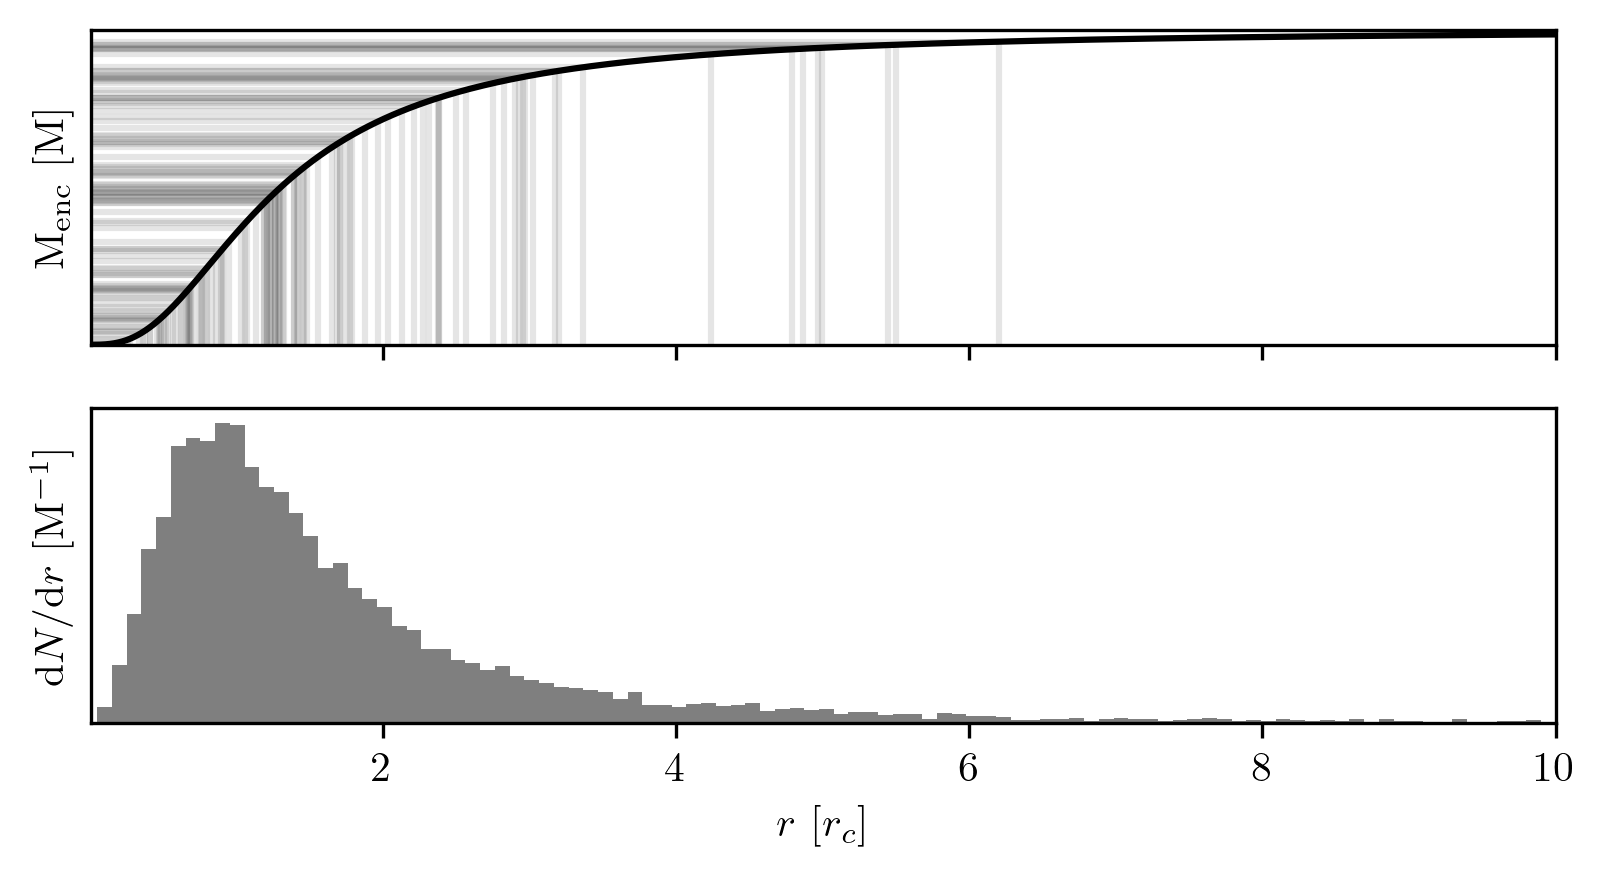
\includegraphics[width=\linewidth]{images/inverse_transform_sampling_distances.png}
                \caption{Inverse transform sampling of the enclosed mass distribution of a Plummer sphere. One thousand uniform random numbers between [0,1] were generated and intersected with the normalized enclosed mass profile. The top panel shows the sampling of positions; only 100 samples are shown to avoid overcrowding. The bottom panel shows the resulting distribution of radial distances.}
                \label{fig:inverse_transform_sampling_distances}
            \end{figure}

            The joint distribution function can be written as the product of a conditional and a marginal distribution: $f(r,v) = f(v|r) f(r)$. The number of particles at a given speed can be obtained by integrating over the angular velocity components and differentiating with respect to speed:
            \begin{equation}
                \frac{dN}{dv} = \frac{d}{dv} \int f(\textbf{v}|r)\, v^2 \sin\theta\, d\theta\, d\phi\, dv = 4\pi v^2 f(v|r).
            \end{equation}

            To construct the CDF of this conditional distribution, we must determine the appropriate limits. The allowed speed for a particle at radius $r$ ranges from zero to the escape speed, $v_{\mathrm{esc}} = \sqrt{2\Phi(r)}$. The resulting CDF is:
            \begin{equation}
                \mathcal{F}(v) = C \int_0^{v < v_\mathrm{esc}} 4\pi v^2 f(v|r) dv,
            \end{equation}
            where $C$ is a normalization constant. Although I do not present an analytical expression for $C$, it is straightforward to normalize numerically. In practice, I omit multiplicative constants and normalize a posteriori using:
            \begin{equation}
                C = \frac{1}{\mathcal{F}(v_\mathrm{esc})}.
            \end{equation}

            Sampling the speeds is shown in Fig.~\ref{fig:inverse_transform_sampling_velocities}. Since this is a conditional distribution, each particle has its own CDF based on its position—unlike Fig.~\ref{fig:inverse_transform_sampling_distances}, where all particles are sampled from the same marginal distribution. Note that for particles located farther from the center, fewer speeds are available before they become unbound.

            \begin{figure}
                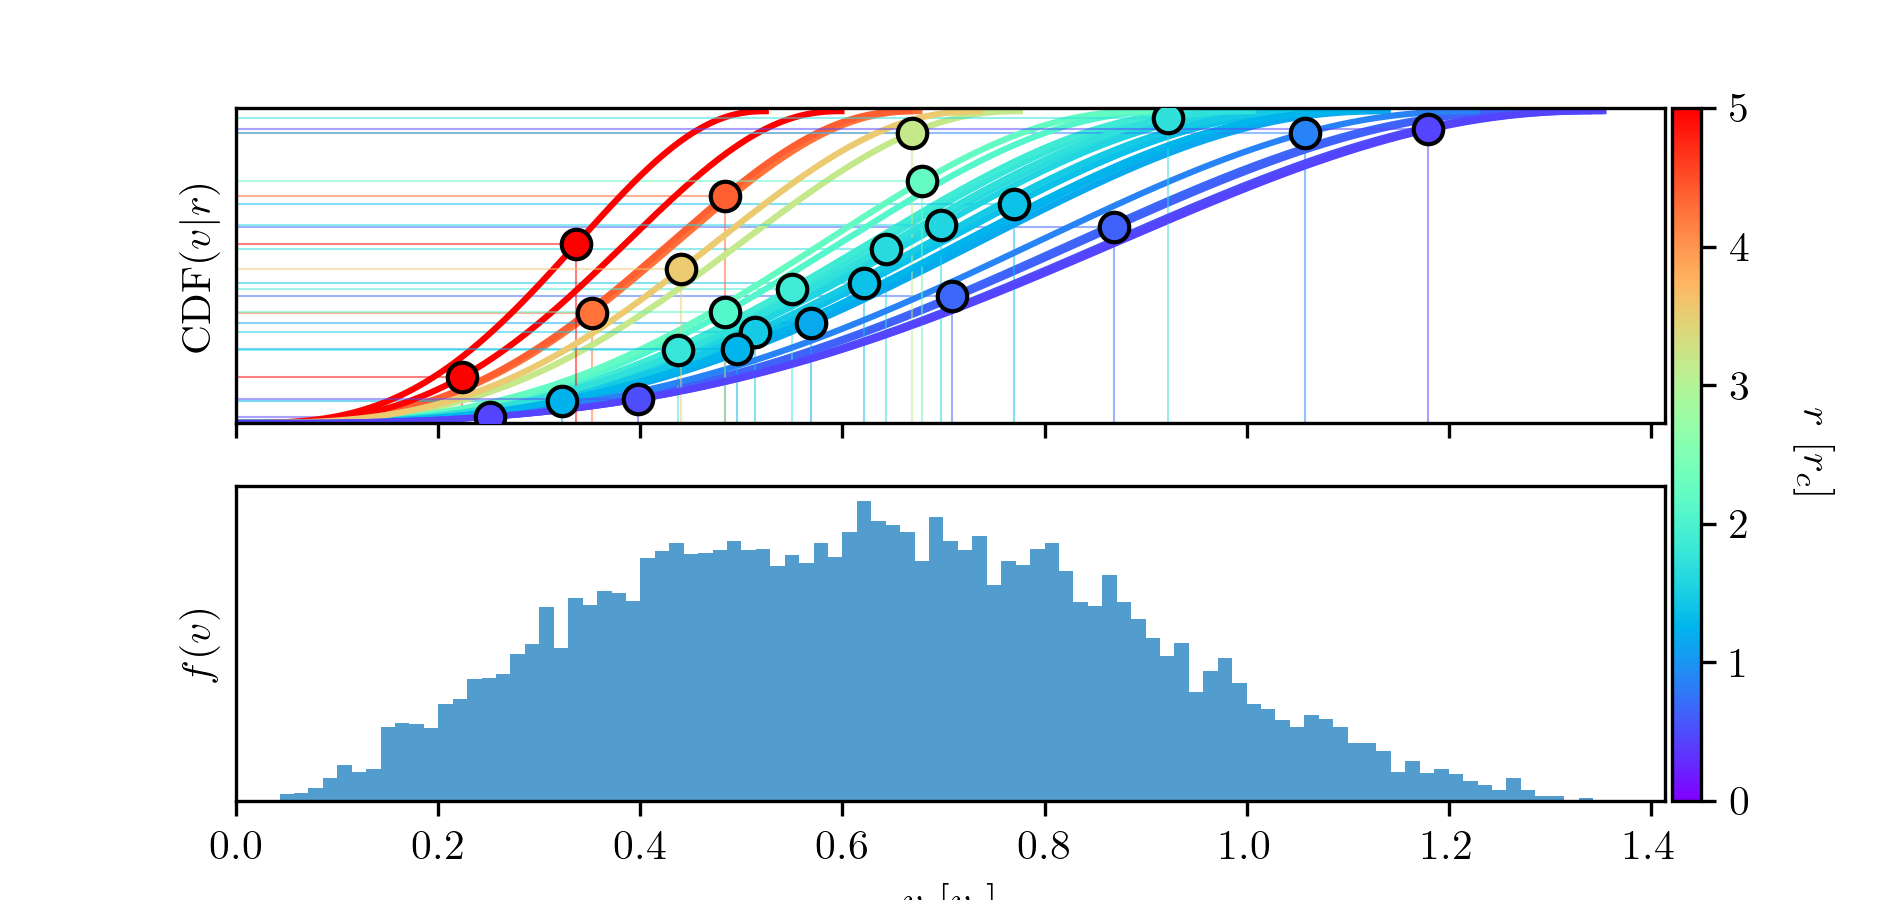
\includegraphics[width=\linewidth]{images/inverse_transform_sampling_velocities.png}
                \caption{Inverse transform sampling of the speed distribution conditioned on position for particles in a Plummer sphere ($N = 1000$). The top panel shows 25 samples (to avoid clutter), each colored by its sampled distance. For each particle, a uniform random number is mapped onto its corresponding CDF to obtain the speed. The bottom panel shows the distribution of sampled speeds. The theoretical maximum value, corresponding to the escape speed at the center, is $\sqrt{2GM/r_c}$.}
                \label{fig:inverse_transform_sampling_velocities}
            \end{figure}

            This process could be inverted: one could marginalize over position to obtain a global speed distribution, then condition on speed to sample positions. While valid, this approach is less intuitive. Most models are motivated by their density profiles, which are observable and conceptually accessible, making them a natural starting point for inverse transform sampling.
            
            To convert radial distances into 3D positions, and speeds into velocity vectors, we must sample directions uniformly over the surface of a sphere. A common pitfall is to sample latitude and longitude uniformly, which leads to an over-density near the poles. Instead, we aim for a uniform distribution over the sphere's surface, where the differential area element is given by:
            \begin{equation}
                f(\theta,\phi)=\frac{1}{4\pi}\sin(\theta)
            \end{equation} 
            with $\theta$ the co-latitude and $\phi$ the longitude. Since $f$ does not depend on $\phi$, it can be sampled uniformly over its domain $[0, 2\pi)$. However, for $\theta$, inverse transform sampling must be used. Drawing a uniform random variable $y_i \in [0,1]$, the corresponding co-latitude is:
            \begin{equation}
                \theta_i = \cos^{-1}\left(1-2y_i\right).
            \end{equation}

            By sampling radial distances, speeds, and directions uniformly over the unit sphere, we obtain full position and velocity vectors for each particle. With these, the initial conditions for a Plummer sphere are fully specified. The user need only provide the total mass, characteristic radius, and the desired number of star particles.


            With the equations of motion defined, a model for the galactic gravitational field established, a force model for the globular cluster in place, and initial conditions assigned to each star particle, we are now ready to simulate the tidal disruption of a globular cluster in the Galaxy.



\section{The Implicit Physics}
    The previous section provided everything needed to simulate the dissolution of globular clusters. However, given the equations of motion, the model for the gravitational field, and the initial conditions for both the globular clusters and their constituent stars, why should we expect stars to escape? While the formalisms in the previous section supply the necessary machinery for running simulations, they do not explain \textit{why} disruption occurs.

    In this section, I aim to describe the underlying mechanisms that cause stars to escape from globular clusters and form stellar streams. Gaining intuition for this process involves simplifying the equations \textit{even further}, in order to obtain analytical insights. I refer to this as the \textit{implicit physics}—not because it was explicitly implemented in the simulations, but because it arises naturally from the equations that be.

    To provide a brief overview: I begin with the circular restricted three-body problem, the simplest formalism for understanding the kinds of motion a massless body can undergo when influenced by two much more massive ones. I then introduce the tidal tensor, which describes how and why the galactic field eventually strips stars from their host clusters. After that, I discuss phase mixing, which explains the evolution of escaped stars and how they come to form coherent stellar streams. This also helps explain the divergence of orbital solutions over time, which is particularly relevant for the work in Chapter~5, where we investigate whether the globular cluster system can affect the Palomar~5 stream. Finally, I introduce \textit{gapology}—the study of how perturbations can impact a stream and generate observable gaps within it.

    
    \subsection{The Planar Circular Restricted Three-Body Problem}
        
        This section introduces the fundamental concept of the Lagrange points and regions of influence. In general, if a star is very close to the center of mass of a globular cluster, then its dynamics are determined by the cluster and the galaxy's influence is minimal. On the otherhand, if the star is far from the cluster then its motion is completely describe by the galaxy's gravitational field and the cluster is completely negligible. The Lagrange points are transitions between these two regime and are the points out of which the stars escape from the cluster. The magic that makes this analysis possible is decoupling the motion of the smallest body from the larger two, and studying the system in a non-inertial reference frame. 

        To begin, even though we simplify the simulation by modeling the cluster as $\mathcal{N}$ independent three-body problems, the problem remains challenging. Indeed, if we consider all three bodies to have mass, we can write down a Hamiltonian with 18 dimensions: three positions and three momenta in $\mathcal{R}^3$ for each particle. The dimensionality of the problem can be reduced by using the conservation of total linear momentum and total angular momentum, and by expressing the dynamics in terms of relative coordinates about the system's center of mass. This reduces the total dimensionality to 9. Nevertheless, the problem remains analytically intractable due to its high dimensionality. To gain analytical insight, we simplify the system further.
        
        Instead of writing the full Lagrangian for the three-body motion, we focus on the third particle subject to the gravitational influence of the two massive bodies, in an inertial reference frame centered at the system's center of mass. The Lagrangian then contains the kinetic energy of the third particle and two gravitational potential energy terms from the primary and secondary. However, since the positions and momenta of the primaries are not treated as dynamical variables in our system, they appear as explicit functions of time, making the Lagrangian non-autonomous. This implies that the corresponding Hamiltonian is time-dependent and the total energy of the third particle is not conserved, as the primaries can exchange energy with it.

        We introduce a further simplifying assumption: the two primaries move on circular orbits. Under this assumption, we transform to a reference frame rotating with the primaries, placing them along the $x-$axis. In this rotating frame, the Lagrangian becomes autonomous; it no longer depends explicitly on time and requires no external information to determine the particle's subsequent motion.

        Two effects make this possible. First, by moving to the rotating frame, we introduce non-inertial forces: the Coriolis force and the centrifugal force. The centrifugal force is conservative, associated with a scalar potential. The Coriolis force depends on the particle's velocity as $2\omega\times v$, but because it is always perpendicular to the velocity, it does no work and thus does not change the particle's kinetic energy. After performing the coordinate transformation, the canonical momenta—now position-dependent—can be derived. The resulting Hamiltonian is:
        \begin{equation}
            \mathcal{H} = \frac{1}{2}\left(\left(p_x + \omega y\right)^2 + \left(p_y - \omega x\right)^2 \right) + \Phi_\mathrm{eff}(x,y),
        \end{equation}
        where
        \begin{equation}
            \Phi_\mathrm{eff}(x,y) = -\frac{1}{2} \omega^2 (x^2 + y^2) - \frac{G m_1}{|r_1|} - \frac{G m_2}{|r_2|}.
        \end{equation}

        The potential can be normalized by noting that the orbital angular velocity from the two-body problem satisfies \(\omega^2 = \frac{G M}{a^3}\), where \(a\) is the separation between the primaries and \(M = m_1 + m_2\) is the total mass of the system. With this normalization, the system depends on a single dimensionless parameter \(\mu\), the relative mass ratio defined as \(\mu = \frac{m_2}{m_1 + m_2}\).

        At this point, the system can be studied qualitatively. Unfortunately, no general closed-form solution exists for the circular restricted three-body problem that describes the subsequent motion as a function of time. However, by studying the effective potential \(\Phi_\mathrm{eff}\), we gain valuable insights.

        Our Hamiltonian depends on the four variables \((x, y, p_x, p_y)\) and has one integral of motion.\footnote{The term ``integral of motion'' is often used interchangeably with ``constant of motion'', but strictly speaking, the latter is preferable since it refers to a quantity that remains constant throughout the orbital evolution, not to an integral in the mathematical sense of the word (area under a curve).} A famous quantity in this context is the Jacobi integral (or Jacobi constant), often written as \(C_j = -2E\). Defining this constant is somewhat arbitrary since the total mechanical energy \(E\) is itself conserved, and any scalar multiple of it is also conserved. The utility of the Jacobi constant is mostly conventional: it is often defined to be positive and multiplied by 2, which simplifies the expression for forbidden regions and zero-velocity curves. For example, one can write
        \[
        \dot{x}^2 + \dot{y}^2 = 2 \Phi_\mathrm{eff}(x,y) + C_j,
        \]
        instead of the equivalent
        \[
        \dot{x}^2 + \dot{y}^2 = -2 \Phi_\mathrm{eff}(x,y) + 2E.
        \]
        

        Since we have four variables and one constraint, the motion is restricted to a three-dimensional hypersurface (or manifold) embedded in the four-dimensional phase space.

        At this stage, we find the points where \(\nabla \Phi_\mathrm{eff} = 0\), which correspond to the Lagrange points—locations where all effective forces balance. Of particular importance are the first two Lagrange points \(L_1\) and \(L_2\), which lie along the line connecting the primary and secondary. The effective potential at \(L_1\) is lower than at \(L_2\).

        Given a certain energy level, setting the kinetic energy to zero defines boundaries between regions where the particle can and cannot move. Regions where the kinetic energy would have to be negative (which is physically impossible) are forbidden, since that would require imaginary velocities.

        The points \(L_1\) and \(L_2\) are especially important for our study of a globular cluster with stars initially bound to it. Stars can escape through these Lagrange points: lower-energy particles tend to escape through \(L_1\), while higher-energy particles can also escape through \(L_2\). Figure~\ref{fig:CR3BP_forbidden_region} illustrates these forbidden and allowed regions clearly.




        \begin{figure}
            \centering
            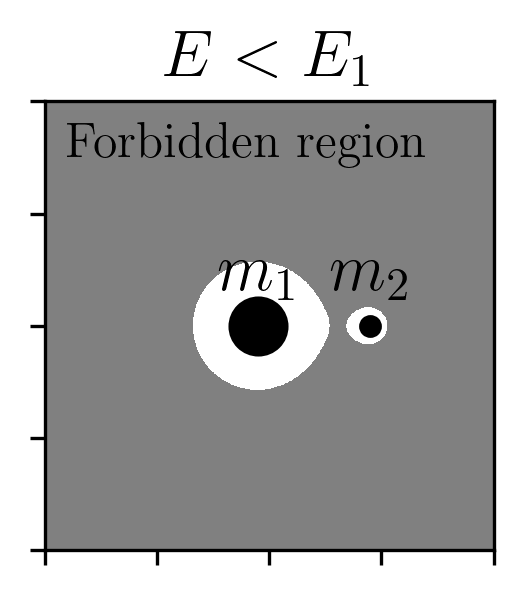
\includegraphics[width=.32\linewidth]{images/CR3BP_forbidden_region_0.png}
            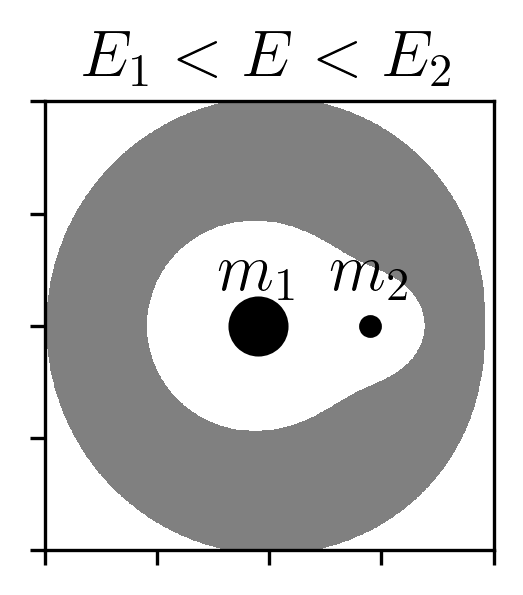
\includegraphics[width=.32\linewidth]{images/CR3BP_forbidden_region_1.png}
            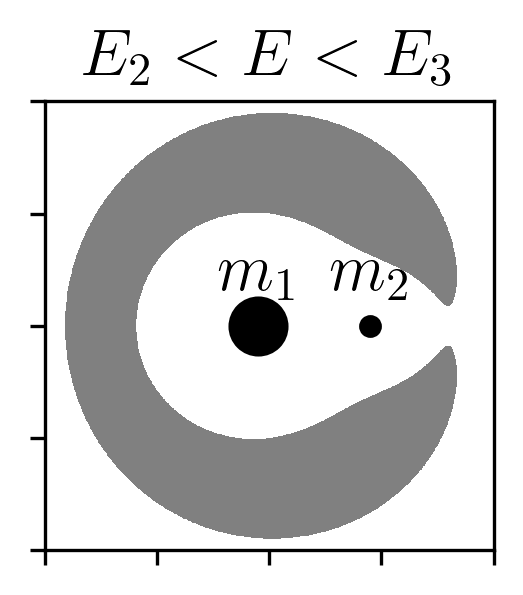
\includegraphics[width=.32\linewidth]{images/CR3BP_forbidden_region_2.png}
            
            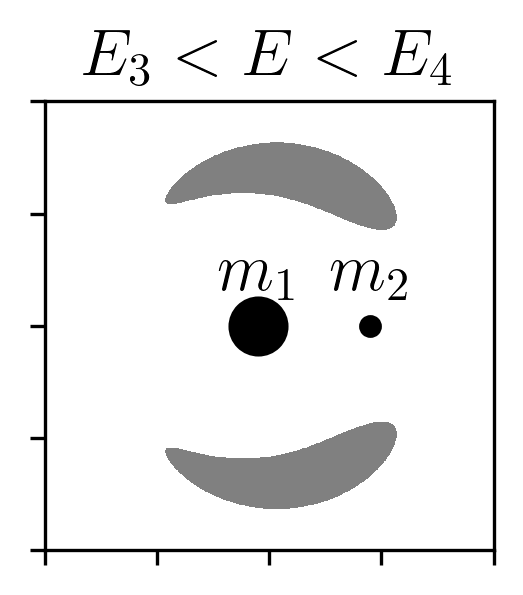
\includegraphics[width=.32\linewidth]{images/CR3BP_forbidden_region_3.png}
            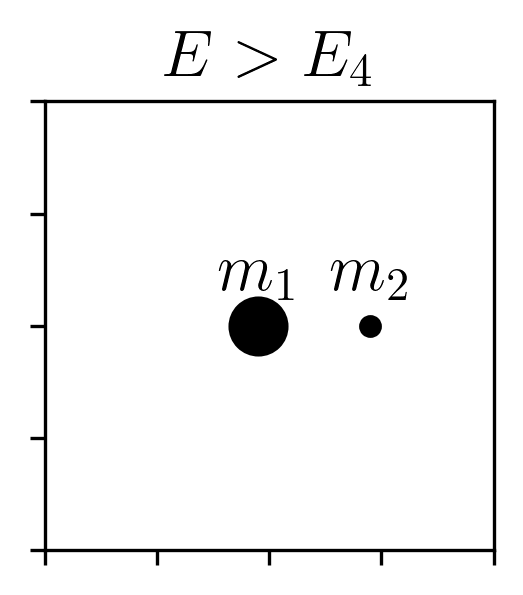
\includegraphics[width=.32\linewidth]{images/CR3BP_forbidden_region_4.png}
            \caption{A reproduction of Fig.~2.4.2 from \citet{koon2000dynamical}. Each plot is shown in the non-inertial reference frame rotating with the orbital frequency of the primary and secondary about their common center of mass. In this example, the mass ratio is \(m_1 = 10 m_2\). The gray regions represent areas inaccessible to the test particle for a given energy. In the first case, where \(E < E_1\), the particle remains confined to orbit either around the primary or the secondary, depending on its initial position. As the particle's energy increases, more of the \(xy\)-plane becomes accessible. The narrow passage between \(m_1\) and \(m_2\) corresponds to the \(L_1\) Lagrange point, while the choke point allowing escape to the exterior when \(E > E_2\) is the \(L_2\) point.}
            \label{fig:CR3BP_forbidden_region}
        \end{figure}

        The distance from the secondary to the first and second Lagrange points is approximately equal, defining a region around the secondary known as the Hill sphere. Within this zone, the gravitational influence of the secondary dominates over that of the primary. The Hill radius is commonly approximated as \( r_h \approx r\sqrt[3]{m_2/m_1} \), where \( r \) is the separation between the primaries. Interestingly, the expression for the Hill radius arises from a fifth-order polynomial expansion of the effective potential—a detail that might seem minor, but is actually quite delightful. In most areas of physics, approximations typically emerge from Taylor expansions, basis function decompositions, or limits where the governing equations simplify.

        At conferences, we have been asked whether we have ever observed \textit{recapture}—that is, a star particle leaving a globular cluster and eventually returning. If the system were as simple as the circular restricted three-body problem, recapture could occur for star particles with energies in the range \( E_1 < E < E_2 \) or \( E_2 < E < E_3 \). In such cases, depending on initial conditions, a particle might orbit the secondary, escape, and later return.

        However, in our simulations, the galaxy and globular clusters are not treated as point masses, and the clusters follow eccentric, inclined, and non-closed orbits. This means the topology of the forbidden region evolves over time. For a particle with a given energy \( E \), it may be unbound at one moment but later find itself within the Hill sphere again, as the potential landscape changes dynamically. Indeed, we have observed such behavior in our simulations.

        The Lagrange points, forbidden regions, and Jacobi energy are powerful concepts which, while they do not rigorously apply in our more complex setup, still offer valuable qualitative insights. In our regime, it is more fruitful to think in terms of tidal forces as the underlying mechanism that gradually transfers energy and angular momentum, nudging stars across Lagrange boundaries and ultimately enabling escape. It is to this process—tidal stripping—that we now turn.

        % \textbf{NOTE from Ferrone. I wonder if the $L_4$ and $L_5$ exist in the galactic context... are there Tojan stars? or does the complexity of the galactic potential paired with non circular orbits render such a phenomena unnatural?}

    \subsection{Tidal Forces}
        For star-particles within a globular cluster that is itself orbiting within a galaxy, there are no exact integrals of motion. The system lacks symmetries in its Lagrangian, and the potential varies with time, so even the orbital energy is not conserved. In such a time-dependent and asymmetric context, it is more insightful to frame the problem in terms of forces rather than conserved quantities. In particular, tidal forces arise when the gravitational field of the galaxy (the primary) is treated as an external perturbation to the field of the globular cluster (the secondary). In this section, I aim to build an intuitive and formal understanding of tidal forces, framing them as tensor quantities. We begin with the simplest case—the familiar Sun-Earth system—before extending the discussion to the galactic context. I also provide a broader overview of how tidal forces vary depending on the cluster's orbit within the galaxy.

        To start, tidal forces arise due to spatial variations in the gravitational field with respect to a reference point, which is almost always the secondary body. There are two equivalent optiosn to quanitfy this. The first is to consider a Taylor expansion of the gravitational potential of the primary, \(\Phi_g\), evaluated at the star's position \(\vec{x}_s\), relative to the secondary's position \(\vec{x}_c\):
        \begin{equation}
            \Phi_g\left(\vec{x}_s\right) \approx \Phi_g\left(\vec{x}_c\right) + \left[\nabla \Phi_g (\vec{x}_c)\cdot \Delta \vec{x}\right] + \left[\Delta \vec{x} \cdot \mathcal{D}^2\left(\Phi_g\right) \cdot \Delta\vec{x}\right],
        \end{equation}
        where \(\Delta \vec{x} = \vec{x}_s - \vec{x}_c\), and \(\mathcal{D}^2 \Phi_g\) is the Hessian matrix of second derivatives of the potential: \(\partial^2 \Phi/\partial x_i \partial x_j\).

        the second expression can be derived by linearizing the gravitational force in a non-inertial frame co-moving with the secondary. Let us write Newton's second law for the star-particle and the secondary in an inertial frame:
        \begin{eqnarray}
            \vec{F}_s &= \nabla \Phi_c\left(\Delta \vec{x}\right) + \nabla \Phi_g\left(\vec{x}_s\right),\\
            \vec{F}_c &= \nabla \Phi_g\left(\vec{x}_c\right).
        \end{eqnarray}
        Then the relative acceleration of the star in the non-inertial frame is:
        \begin{eqnarray}
            \vec{f}_s &= \vec{F}_s - \vec{F}_c + \vec{F}_\mathrm{fictitious} \\
                    &= \nabla \Phi_c\left(\Delta \vec{x}\right) + \nabla \Phi_g\left(\vec{x}_s\right) - \nabla \Phi_g\left(\vec{x}_c\right) + \vec{F}_\mathrm{fictitious} \\
                    &\approx \nabla \Phi_c\left(\Delta \vec{x}\right) + \mathrm{Jac}\left(\nabla \Phi_g(\vec{x}_c)\right) \cdot \Delta \vec{x} + \vec{F}_\mathrm{fictitious},
        \end{eqnarray}
        where the last line uses a first-order Taylor expansion of the gravitational force field, valid under the assumption that \(|\Delta \vec{x}| << |\vec{x}_c|\). 

        The Jacobian of the gravitational field is equal to the Hessian of the potential, owing to the symmetry of second derivatives and the fact that \(\vec{g} = -\nabla \Phi_g\). This matrix, known as the \textit{tidal tensor} \(\mathcal{T}\), describes the linearized spatial variation of the gravitational field:
        \begin{equation}
            \mathcal{T} = -\mathcal{D}^2\Phi_g = \mathrm{Jac}(\nabla \Phi_g) = \left(\begin{matrix}
                \partial_x g_x & \partial_y g_x & \partial_z g_x \\
                \partial_x g_y & \partial_y g_y & \partial_z g_y \\
                \partial_x g_z & \partial_y g_z & \partial_z g_z 
            \end{matrix}\right).
        \end{equation}

        While the Hessian and Jacobian are formally equivalent, the Jacobian viewpoint offers a more geometric interpretation: it acts as a linear transformation on nearby displacements, mapping them to differences in acceleration. Diagonalizing the tidal tensor reveals the principal axes of tidal deformation. A positive eigenvalue corresponds to stretching along the associated eigenvector; a negative eigenvalue indicates compression. The magnitude gives the rate of stretching or compression.

        Finally, we note that although many relevant potentials exhibit spherical or cylindrical symmetry, Cartesian coordinates are preferred here. In curvilinear systems, computing the Jacobian or Hessian requires accounting for Christoffel symbols, which complicates the interpretation and computation.
        
        \subsubsection{The Moon}
            Nothing clarifies the concept of tides like the most familiar example: the Moon. Tidal forces are invoked to explain a wide range of phenomena in the Earth-Moon system. The most relatable effect is, of course, the periodic variation in sea level on Earth. While accurately modeling these changes requires fluid dynamics—beyond the scope of this thesis—NASA provides several accessible explanations and visualizations at \href{https://science.nasa.gov/moon/tides/}{https://science.nasa.gov/moon/tides/}, including daily high and low tides, as well as spring and neap tides.

            Another key example is the tidal deformation of the Moon, which ultimately led to its tidal locking—explaining why we always see the same side of the Moon from Earth.

            A particularly insightful illustration is the angular offset between the Earth's tidal bulge and the Moon's position, caused by the Earth's rotation. This offset results in a torque that transfers angular momentum from the Earth's rotation to the Moon's orbit. As a consequence, Earth's rotation gradually slows while the Moon slowly recedes from Earth. 
            
            All of the above phenomena requires using the tidal tensor for a Keplerian potential:
            \begin{equation}
                \mathcal{T}= -\frac{GM}{r^3}\left(\begin{matrix}
                    1-\frac{3x^2}{r^2} & -\frac{3xy}{r^2} & -\frac{3xz}{r^2} \\
                    -\frac{3yx}{r^2} & 1-\frac{3y^2}{r^2} & -\frac{3yz}{r^2} \\
                    -\frac{3zx}{r^2} & -\frac{3zy}{r^2} & 1-\frac{3z^2}{r^2}
                \end{matrix}\right),
            \end{equation}
            which has eigenvalues $2\frac{GM}{r^3}$, $-\frac{GM}{r^3}$, and $-\frac{GM}{r^3}$, with corresponding eigenvectors:
            \begin{equation}
                \vec{v}_1,\vec{v}_2,\vec{v}_3 = \dfrac{1}{r}\begin{bmatrix} x \\ y \\ z \end{bmatrix}, \dfrac{1}{r}\begin{bmatrix} -x \\ y \\ 0 \end{bmatrix}, \dfrac{1}{r}\begin{bmatrix} -x \\ 0 \\ z \end{bmatrix}.
            \end{equation}

            Notably, the first eigenvalue is positive and corresponds to a stretching deformation along the position vector. The other two are negative, representing compression in directions perpendicular to the stretching axis. These directions define a plane orthogonal to the Earth-Moon line. 
            
            From this, several tidal effects become evident. For instance, the Earth's oceans stretch along the Earth-Moon axis due to the Moon's tidal forces. While the Sun also exerts tidal forces on Earth, their magnitude is weaker due to the $r^{-3}$ scaling with distance. When the Moon is either full or new, the Sun and Moon's tidal forces act constructively, leading to spring tides. At first and third quarters, they interfere destructively, causing neap tides. Additionally, Earth's tidal influence distorts the Moon from spherical symmetry into an ellipsoid. The Moon's most stable orientation is one where its longest axis aligns with the Earth-Moon line—resulting in tidal locking.

            A more quantitative treatment of these phenomena would require modeling the Moon's internal structure and Earth's ocean dynamics—well beyond the gravity-only scope of this thesis. However, we can still explore one instructive effect: how solar tidal forces \textit{perturb} the Moon's orbit away from the idealized two-body Earth-Moon configuration. Figure~\ref{fig:moon_tidal_simulation} shows a toy model comparing two scenarios. In both, I used initial conditions based on JPL NASA ephemerides \citep{2014IPNPR.196C...1F} and integrated two sets of equations of motion. Neglecting solar tides causes the predicted Moon orbit to drift ahead of the more accurate trajectory. With about three to four years, the two body predicted solution would off by half a moon phase. 

            In the first scenario, the Moon's motion is governed by the two-body Earth-Moon problem with a rotating reference frame correction:
            \begin{equation}
                \ddot{\vec{r}} = -\frac{GM_\oplus}{r^3}\vec{r} - \omega_\oplus \times \left(\omega_\oplus \times \vec{r}_\oplus\right),
            \end{equation}
            while in the second, we include the effect of solar tidal forces:
            \begin{equation}
                \ddot{\vec{r}} = -\frac{GM_\oplus}{r^3}\vec{r} - \omega_\oplus \times \left(\omega_\oplus \times \vec{r}_\oplus\right) -\frac{GM_\odot}{r_\oplus^3}
                \left(\begin{matrix}
                    1-\frac{3x^2}{r_\oplus^2} & -\frac{3xy}{r_\oplus^2} & -\frac{3xz}{r_\oplus^2} \\
                    -\frac{3yx}{r_\oplus^2} & 1-\frac{3y^2}{r_\oplus^2} & -\frac{3yz}{r_\oplus^2} \\
                    -\frac{3zx}{r_\oplus^2} & -\frac{3zy}{r_\oplus^2} & 1-\frac{3z^2}{r_\oplus^2}
                \end{matrix}  \right) \cdot \vec{r},
            \end{equation}
            where $r_\oplus$ is the Earth's position relative to the Sun, $\vec{r}$ is the Moon's position relative to Earth, $M_\odot$ is the mass of the Sun, and $M_\oplus$ is the mass of the Earth. The coordinates $x, y, z$ refer to the components of Earth's heliocentric position.

            \begin{verbatim}
            VIDEO: moon_tidal_simulation.mp4
            \end{verbatim}

            \begin{figure}
                \centering
                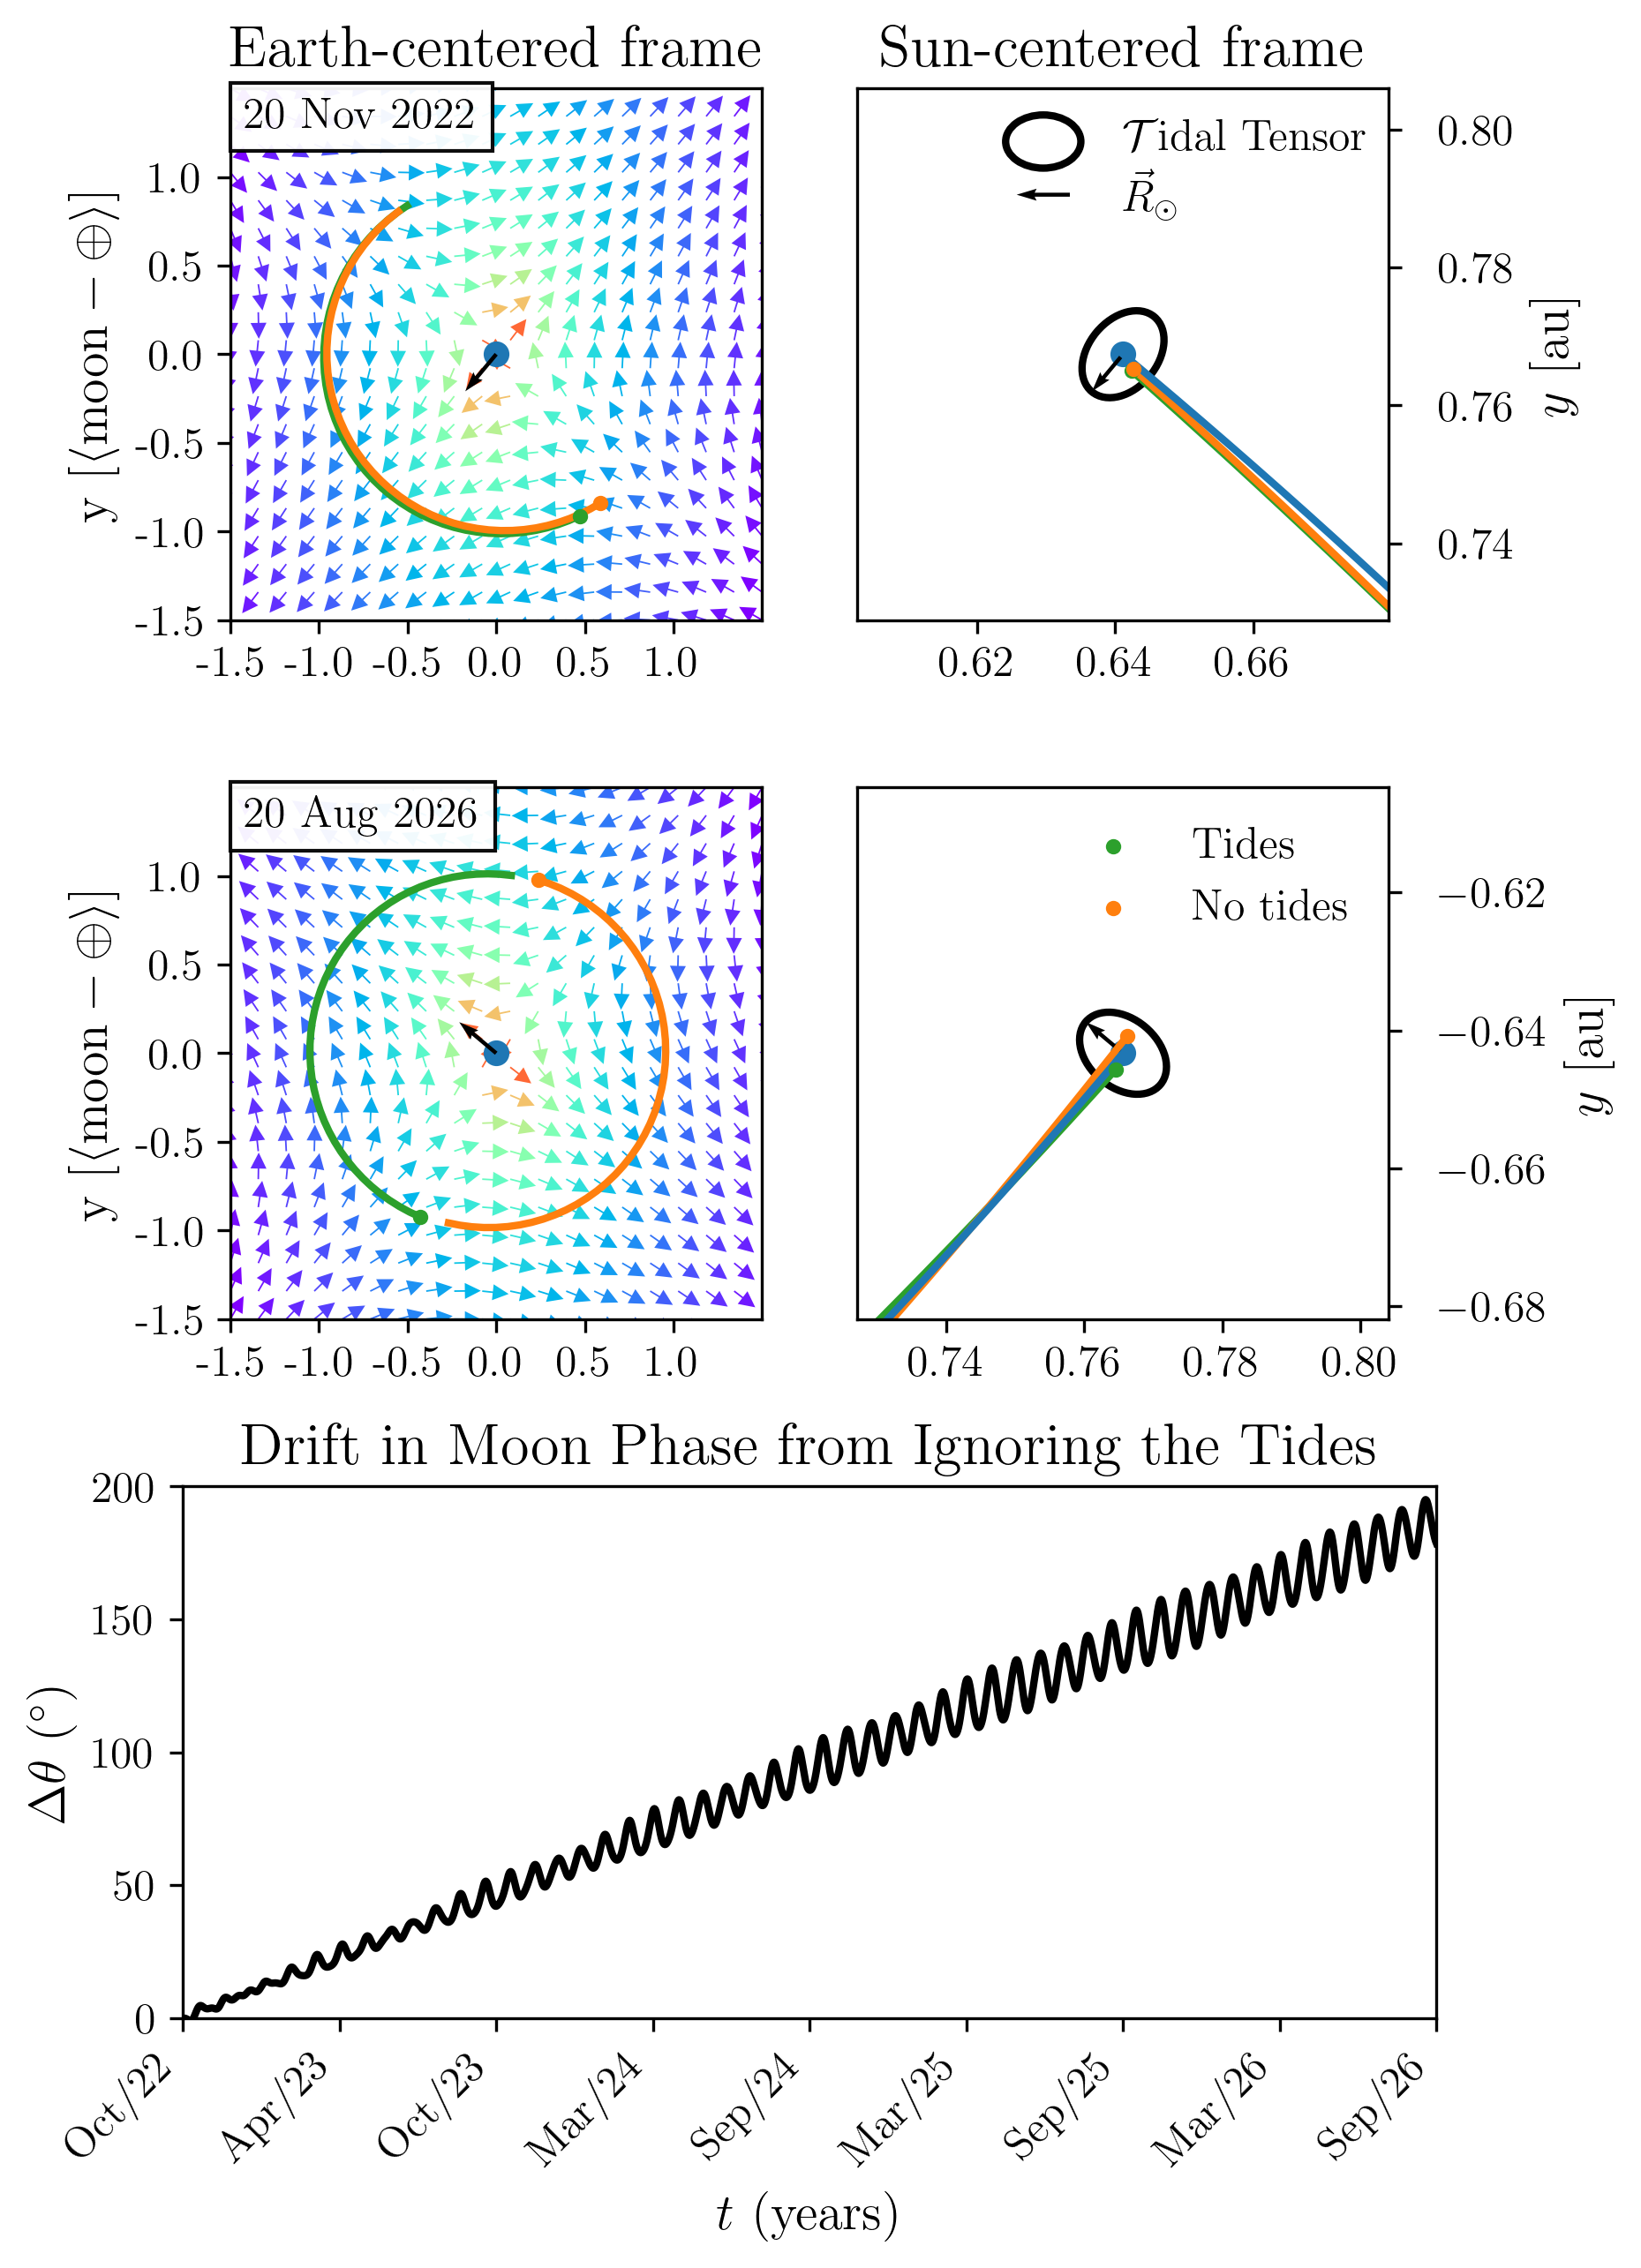
\includegraphics[width=\linewidth]{images/moon_tidal_simulation.png}
                \caption{An illustrative experiment demonstrating the effect of the Sun's tidal field. The left panels show the tidal field, and the right panels show two snapshots of the Moon's orbital trajectory. The green curve include the Sun's tidal effects, while the orange curve corresponds neglects them. The black ellipse represents the tidal ellipsoid, whose major axis aligns with the Sun's position vector relative to the Earth. The bottom panel shows the accumulated phase difference between the two solutions. }\label{fig:moon_tidal_simulation}
            \end{figure}

        \subsubsection{Tides from the disk}
            In the Milky Way, the disk, bulge, and halo each contribute differently to the tidal forces experienced by a globular cluster. The Miyamoto-Nagai disk produces strong, rapidly varying tidal fields near the Galactic plane, leading to phenomena such as disk shocking when clusters cross the disk. The Martos halo, on the other hand, provides a more slowly varying, generally weaker tidal field at large Galactocentric radii.

            The strength and orientation of the tidal field at a cluster's location determine both the rate at which stars are stripped and the geometry of the resulting stellar streams. For example, clusters on eccentric or inclined orbits experience time-dependent tidal forces, with strong compressive shocks during disk crossings and enhanced stretching near pericenter. The eigenvalues and eigenvectors of the tidal tensor at each point along the orbit reveal the principal axes of stretching and compression, which in turn set the directions along which stars are most likely to escape.

            By computing the tidal tensor for the Miyamoto-Nagai disk and Martos halo potentials, as shown below, we can visualize and quantify these effects. The following figures illustrate how the tidal field evolves for representative orbits, highlighting the interplay between the cluster's trajectory and the Galactic mass distribution. This analysis underpins our understanding of stream formation and the morphological diversity of observed tidal tails.

            We can construct the tidal tensor for the Miyamoto-Nagai potential. First, it is convenient to non-dimensionalize the potential. Below, we normalize the potential by the total mass and gravitational constant, $\Phi\prime = \Phi / (GM)$, and each distance by the characteristic length of the disk, $x\prime = x/a$, $b\prime = b/a$. For clarity, we omit the prime notation in what follows. The dimensionless potential then becomes:            
            \begin{eqnarray}
                \Phi   &= \frac{1}{D},\\
                D       &= \sqrt{x^2 + y^2 + \beta^2(z)},\\
                \beta(z)   &= 1 + \sqrt{z^2 + b^2}.
            \end{eqnarray}
            
            % \begin{eqnarray}
                % \beta^{\prime}(z) &= \frac{z}{\sqrt{z^2 + b^2}}\\
                % \beta^{\prime\prime}(z)  &= \frac{b^2}{\left(z^2 + b^2\right)^{3/2}}
            % \end{eqnarray}
            The dimensionless tidal tensor is then: 
            \begin{equation}
                \mathcal{T}=-\frac{1}{D^3}\left(\begin{matrix}
                    1-\frac{3x^2}{D^2} & -\frac{3xy}{D^2} & -\frac{3x\beta \beta'}{D^2} \\
                    \dots & 1-\frac{3y^2}{D^2} & -\frac{3y\beta \beta'}{D^2} \\
                    \dots & \dots & \beta'^2 + \beta \beta'' -\frac{3\left(\beta\beta'\right)^2}{D^2}
                \end{matrix}\right).
            \end{equation}             

            We immediately notice that, due to the cylindrical symmetry, the eigenvectors are not as simple as in the spherical case. As long as 
            \[
            \beta'^2 + \beta \beta'' - \frac{3\left(\beta \beta'\right)^2}{D^2} \neq 1 - \frac{3z^2}{D^2},
            \]
            (1) the stretching axis is no longer parallel to the position vector, and (2) the compression axes do not necessarily lie in the same plane—they may instead be fixed in orientation and differ in magnitude. The exact orientation of all three eigenvectors depends on the cluster's position in the galaxy. Note that if $z = 0$, we recover the case where the stretching eigenvector is parallel to the position vector, although the compression axes remain unequal in magnitude and fixed in orientation. If instead $b = 0$, then we recover spherical symmetry, and the compression eigenvalues become equal.

            \begin{verbatim}
            VIDEO: tidal_deformation_ellipsoid.mp4
            \end{verbatim}

            I have prepared Fig.s~\ref{fig:miyamoto_disc_shocks_circular_inclined_orbit}-\ref{fig:miyamoto_disc_shocks_weak_shocks} to demonstrate the diversity of tidal forces experienced by clusters on various orbits within a Miyamoto-Nagai disk potential. 

            Fig.~\ref{fig:miyamoto_disc_shocks_circular_inclined_orbit} shows a cluster on an inclined, non-eccentric orbit. In contrast, Fig.~\ref{fig:miyamoto_disc_shocks_planar_eccentric_orbit} presents a planar but eccentric orbit. The former experiences repeated disk shocks, while the latter undergoes enhanced tidal forces primarily near pericenter passages.

            Fig.~\ref{fig:miyamoto_disc_shocks_resonant_R_z} presents an orbit in which the radial and vertical oscillation periods are nearly resonant, producing two disk shocks per pericenter passage. Fig.~\ref{fig:miyamoto_disc_shocks_big_apocenter} shows a cluster on an orbit with a large apocenter, resulting in very weak tidal forces overall. Finally, Fig.~\ref{fig:miyamoto_disc_shocks_weak_shocks} demonstrates a case with a very thick disk potential. In this case, disk shocks occur over longer timescales and are less abrupt.

            \begin{figure}
                \centering
                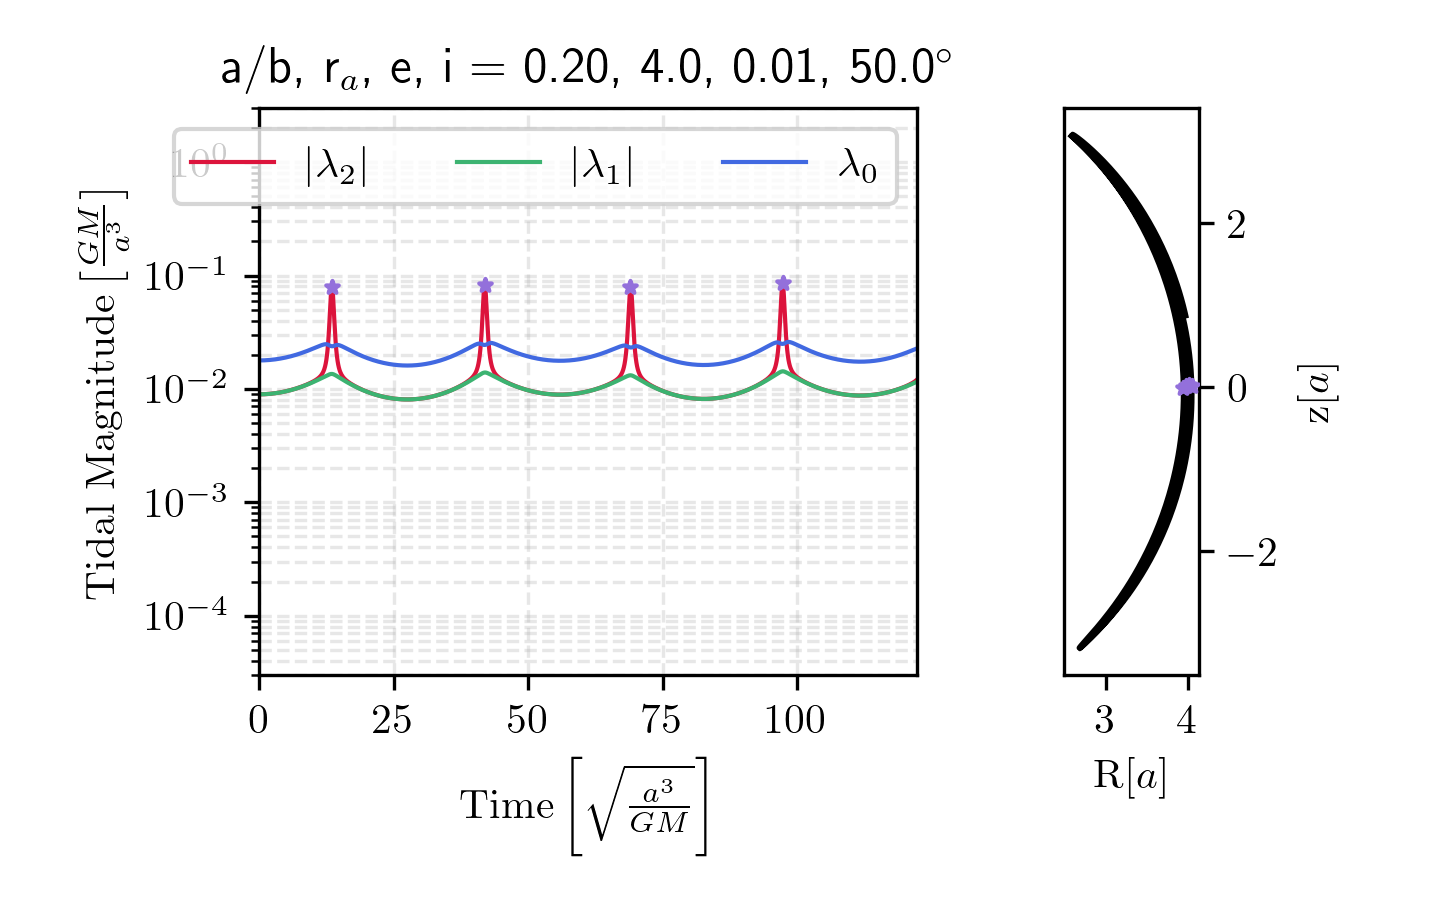
\includegraphics[width=.9\linewidth]{images/miyamoto_disc_shocks_ab_rp_e_i_0.20_4.0_0.01_50.0.png}
                \caption{Tidal forces on an inclined yet non-eccentric orbit. Disk shocks are present, yet there is no tidal stretching from pericenter passages. \textbf{Left}: The three eigenvalues of the tidal tensor matrix are plotted against time. Both the forces and time are normalized to the characteristic values of the Miyamoto-Nagai model, where $a$ is the radial scale length and $M$ is the total mass of the system. The red and green curves correspond to the two compressive axes, while the blue curve shows the magnitude of the stretching axis. The parameters listed at the top describe the orbit: the ratio of cylindrical to vertical scale lengths, the apocenter distance, the eccentricity, and the initial orbital inclination. \textbf{Right}: The orbit is shown in the meridional plane. The purple stars indicate disk crossing events and correspond to the peaks in the magnitude of the eigenvalues. }
                \label{fig:miyamoto_disc_shocks_circular_inclined_orbit}
            \end{figure}

            \begin{figure}
                \centering
                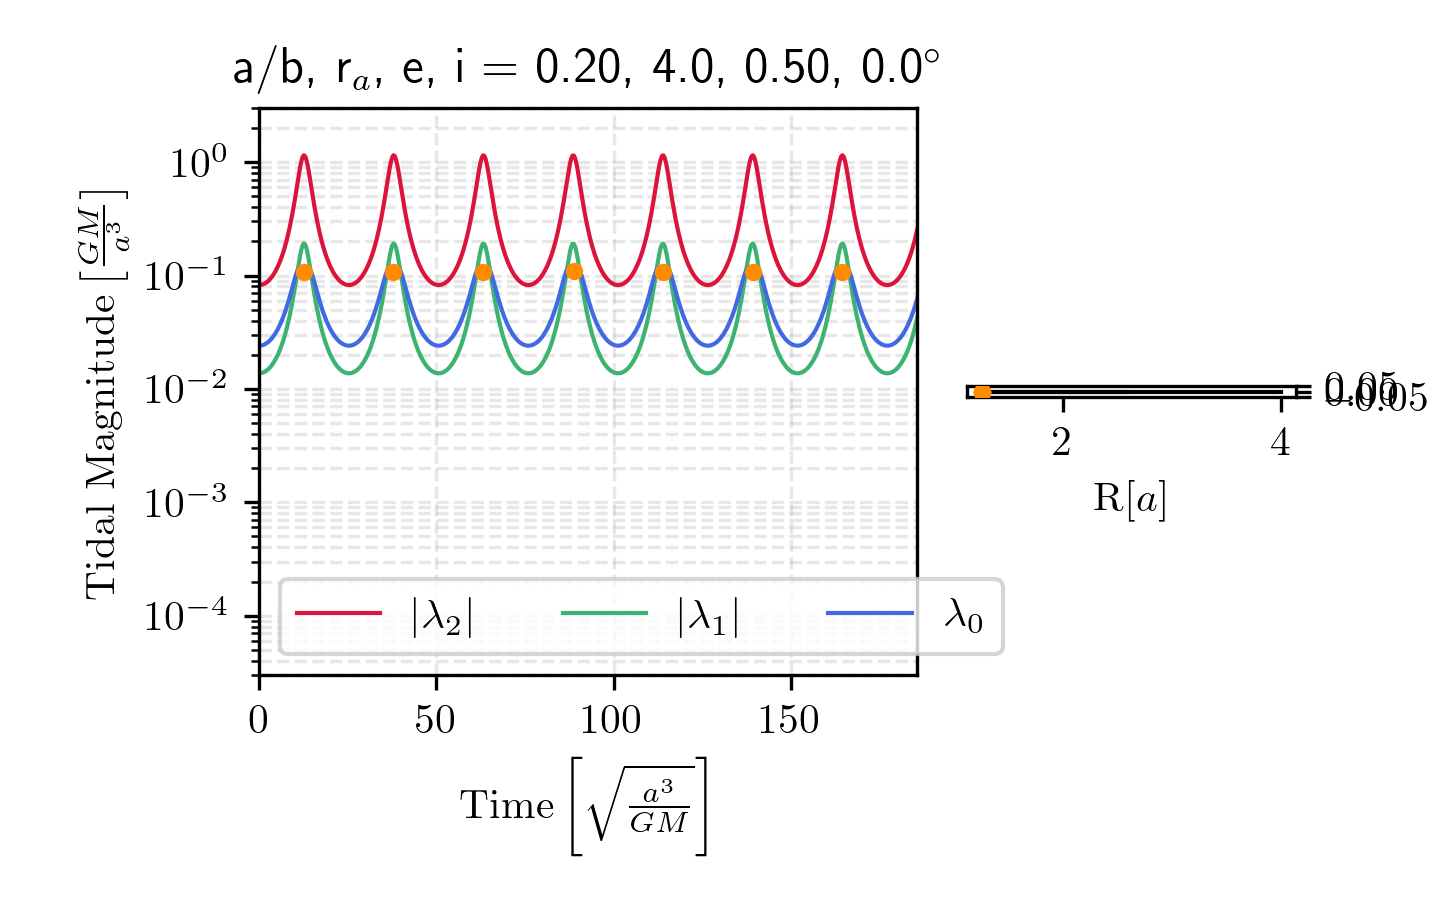
\includegraphics[width=.9\linewidth]{images/miyamoto_disc_shocks_ab_rp_e_i_0.20_4.0_0.50_0.0.png}
                \caption{Evolution of the tidal eigenvectors for an eccentric, non-inclined orbit, resulting in a compressed meridional plane. Orange dots mark the pericenter passages. Since the cluster remains confined to the plane, no disk shocks occur.}
                \label{fig:miyamoto_disc_shocks_planar_eccentric_orbit}
            \end{figure}

            \begin{figure}
                \centering
                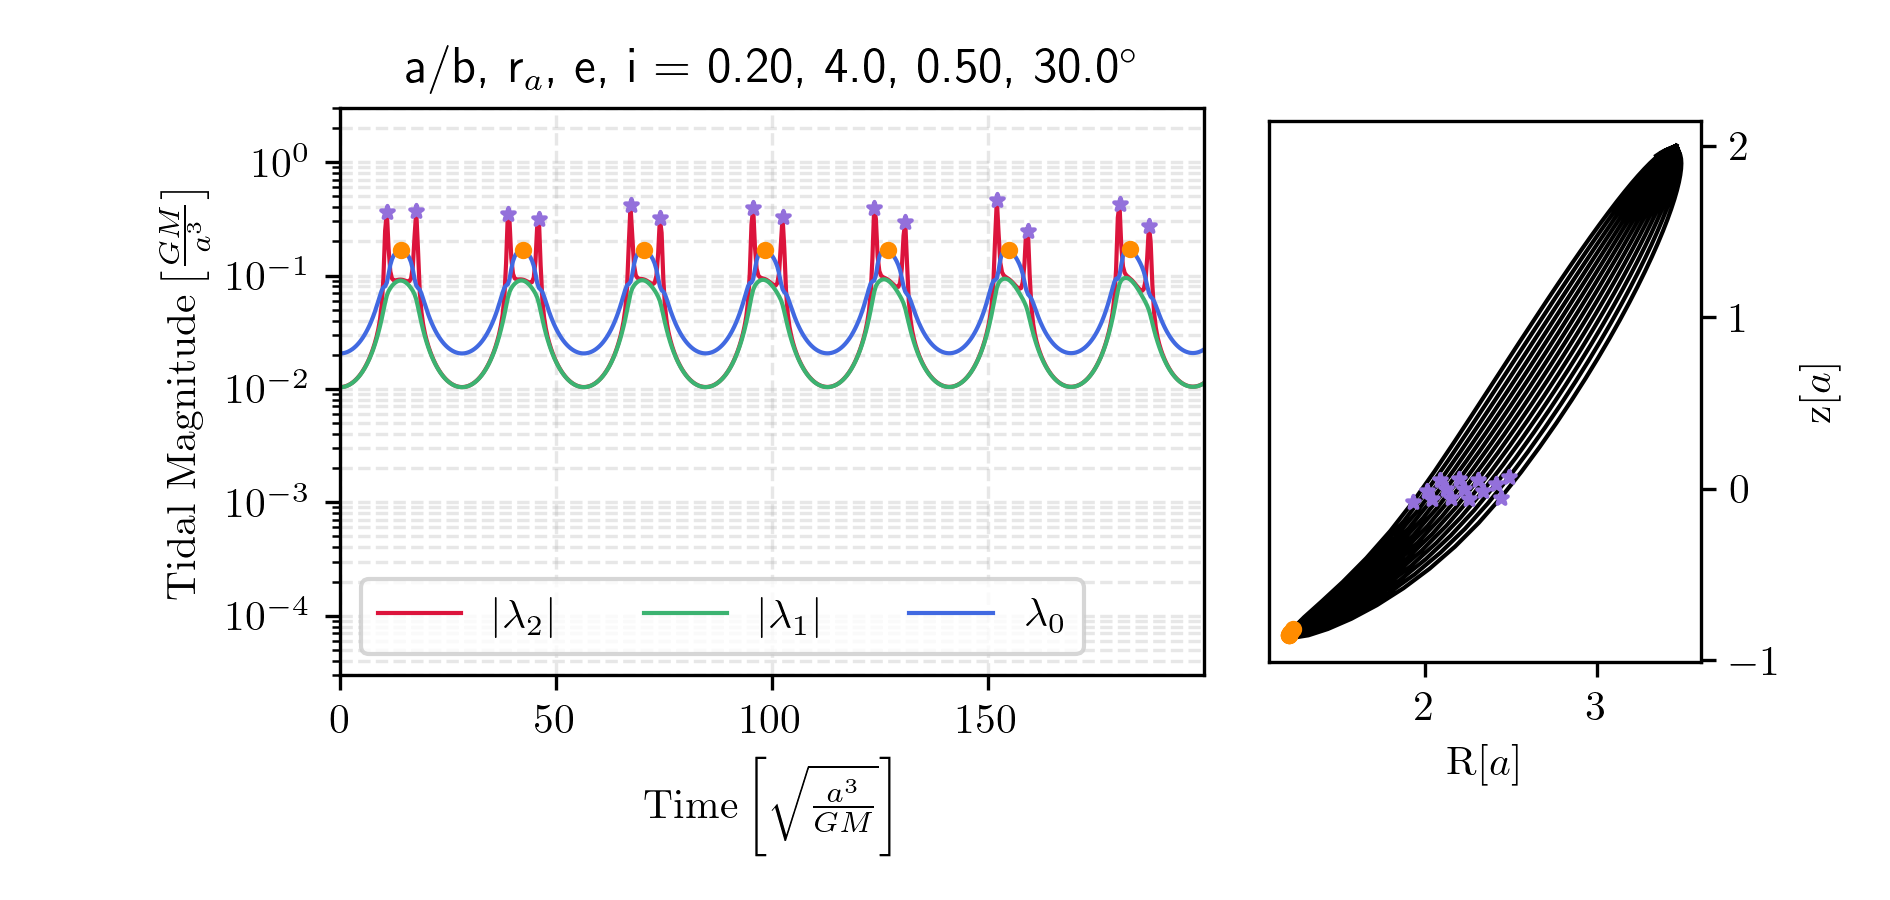
\includegraphics[width=.9\linewidth]{images/miyamoto_disc_shocks_ab_rp_e_i_0.20_4.0_0.50_30.0.png}
                \caption{An inclined, eccentric orbit in which the frequencies in both the $R, p_R$ and $z, p_z$ planes are nearly resonant. The cluster crosses the disk just before and just after each pericenter passage. This is the same orbit as the video presented in this section that is available in the online version.}
                \label{fig:miyamoto_disc_shocks_resonant_R_z}
            \end{figure}
            
            \begin{figure}
                \centering
                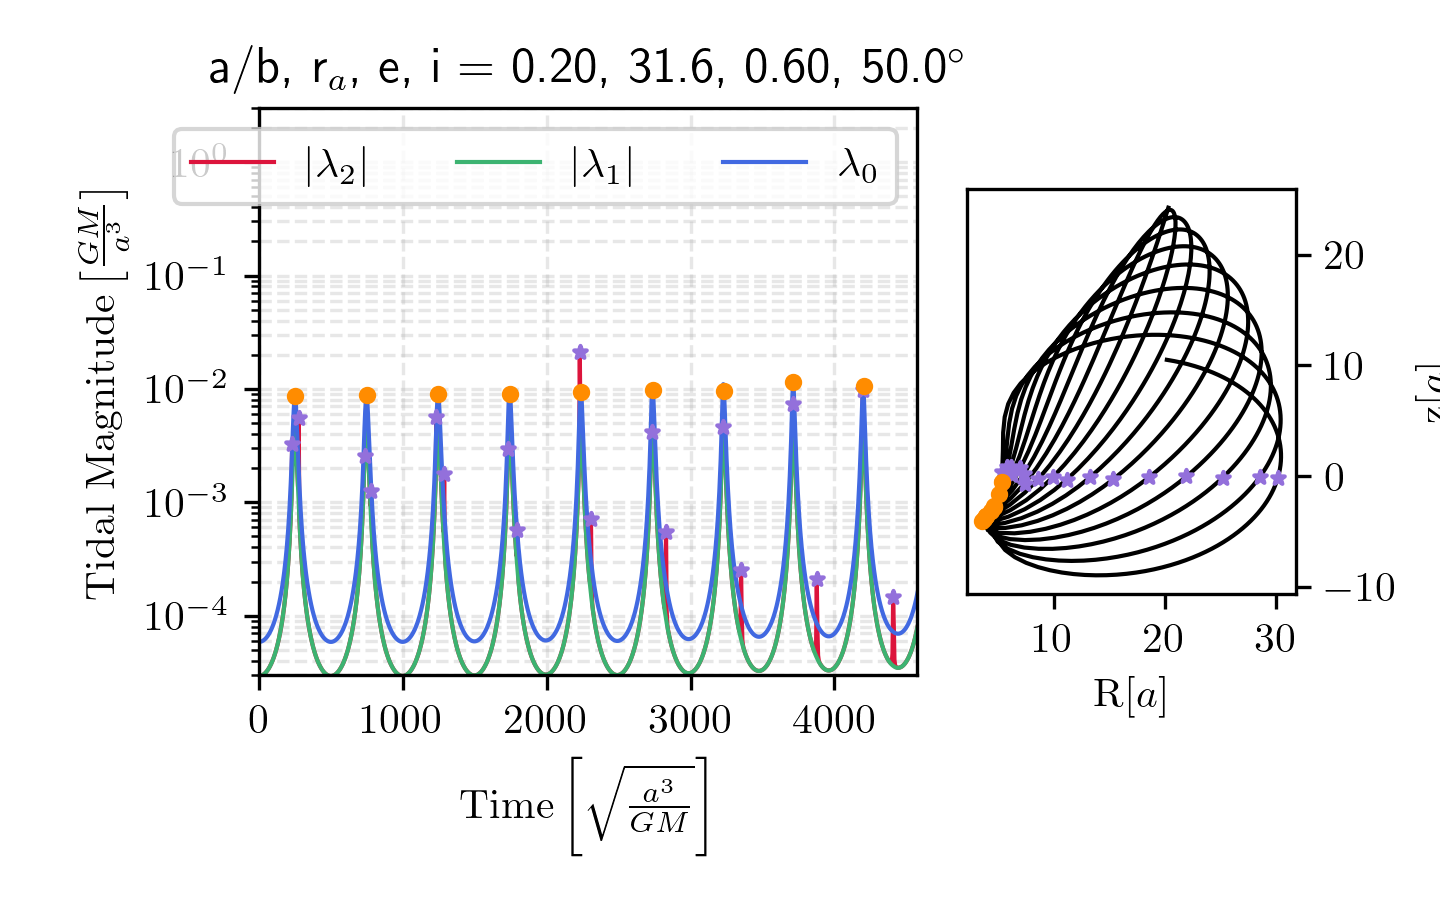
\includegraphics[width=.9\linewidth]{images/miyamoto_disc_shocks_ab_rp_e_i_0.20_31.6_0.60_50.0.png}
                \caption{An eccentric, inclined orbit with a large apocenter. As the cluster evolves through phase space, disk crossings that occur farther out happen at steeper angles and in lower-density regions, reducing the strength of the resulting disk shocks. In contrast, crossings near pericenter remain strong. Because this orbit has higher energy than the previous cases, the overall magnitude of the tidal forces is lower. }
                \label{fig:miyamoto_disc_shocks_big_apocenter}
            \end{figure}
            
            \begin{figure}
                \centering
                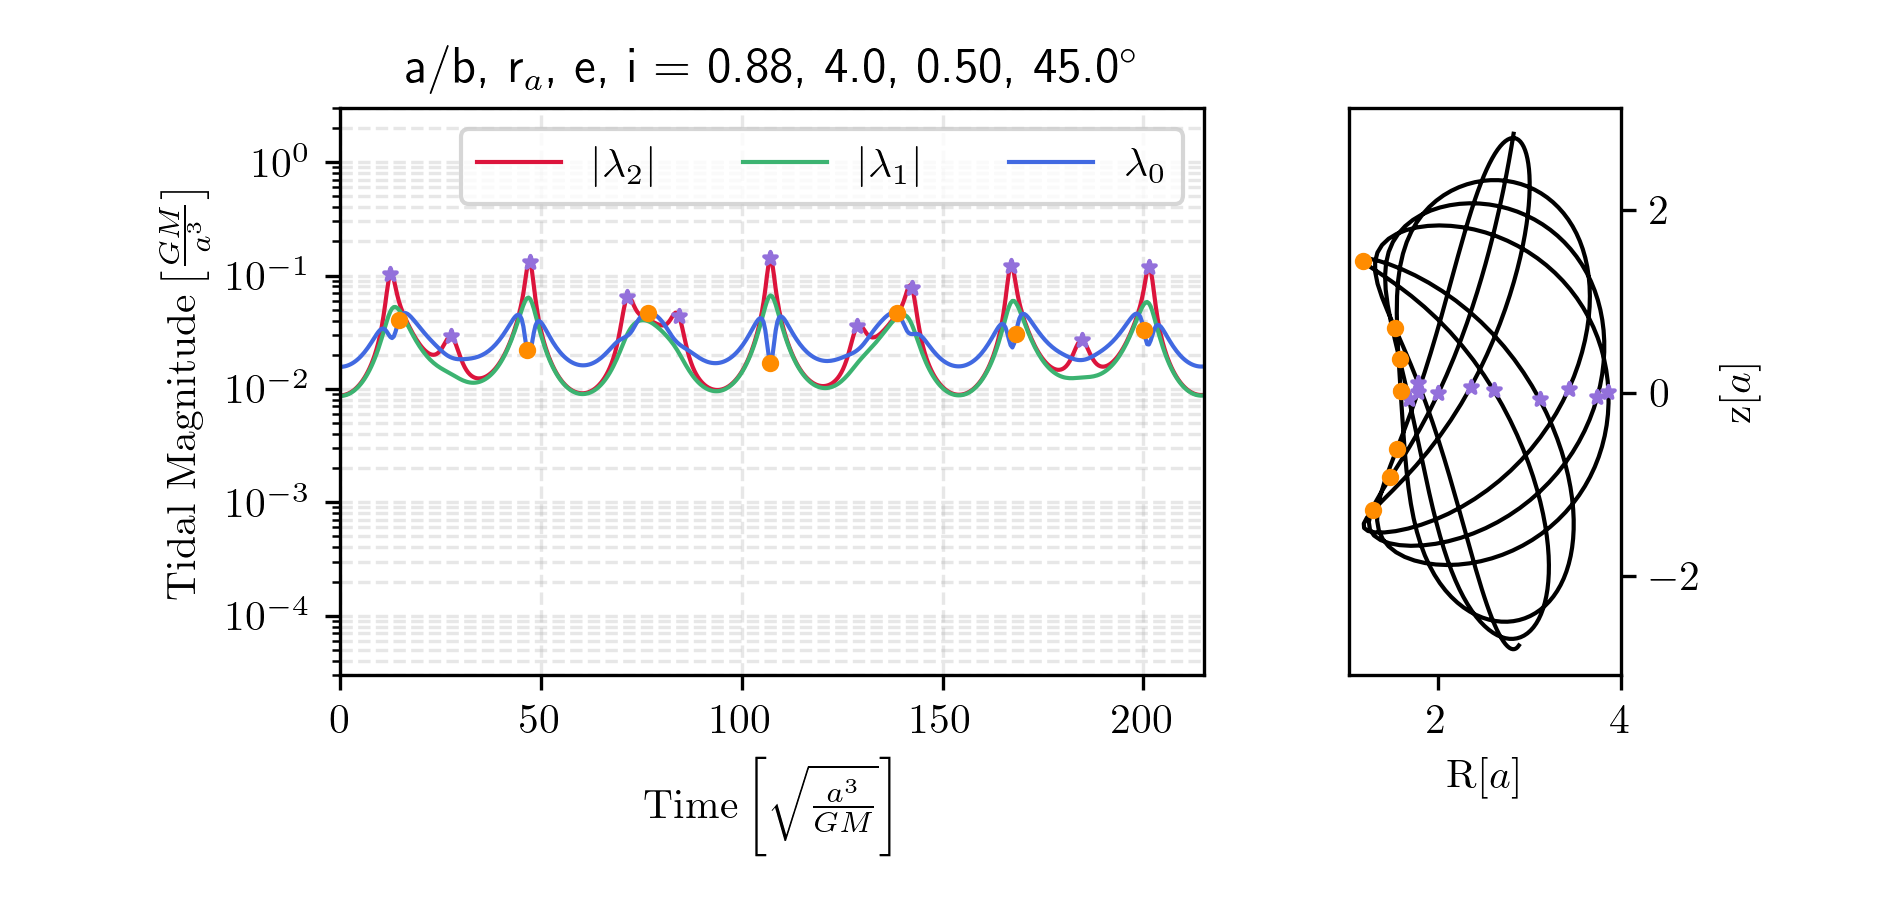
\includegraphics[width=.9\linewidth]{images/miyamoto_disc_shocks_ab_rp_e_i_0.88_4.0_0.50_45.0.png}
                \caption{Eccentric and inclined orbit in a weak disk. The ratio of the cylindrical scale length  to characteristic height (a/b) is close to 1. The disk crossings still produce significant tidal compression, but the resulting shocks are broader.}
                \label{fig:miyamoto_disc_shocks_weak_shocks}
            \end{figure}

        \subsubsection{Tides from the halo}

            Given spherical symmetry, the we expect the tidal tensor of the halo to be similar to that of a keplerian tidal tensor. Perhaps the magnitude of the tidal forces will not scale as simply with $\propto r^{-3}$, since the mass is not concentrated in a single point. However, we can still expect the stretching axis to be parallel with the position vector. 
            
            To explore this, first we rewrite the mass distribution of the Martos halo:
            \begin{equation}
                M'_\text{enc}(s) = \frac{s^\gamma}{1+s^{\gamma-1}}
            \end{equation}
            From Poisson's equation in spherical symmetry: the force is: $\nabla \Phi = - M_\mathrm{enc}/r^2$. The dimensionless tidal tensor can be written as: 
            \begin{equation}
                \mathcal{T'}= -\frac{M'_\text{enc}(s)}{s^3}\left(\begin{matrix}
                    1-\frac{x^2}{s^2}f(s) & -\frac{xy}{s^2}f(s) & -\frac{xz}{s^2}f(s) \\
                    -\frac{yx}{s^2}f(s) & 1-\frac{y^2}{s^2}f(s) & -\frac{yz}{s^2}f(s) \\
                    -\frac{zx}{s^2}f(s) & -\frac{zy}{s^2}f(s) & 1-\frac{z^2}{s^2}f(s)
                \end{matrix}\right)
            \end{equation}  
            where 
            \begin{equation}
                f(s) = 2-\frac{\gamma-1}{1+s^{\gamma-1}}.
                \label{eq:martos_f_s}
            \end{equation}

            While exploring this tidal tensor, I came across an interesting area of the parameter space, that I would like to show here. 

            Taking the Martos tidal tensor in Eq.~\ref{eq:martos_f_s}, we can see that for $\gamma > 3$ and $s <  1$, then $f(s)< 0$. Physically, this would be a sphere whose density increases with distance. This is not natural, as, in general, gravity sends the more massive objects towards the center. However, it's fun to indulge in this situation to learn some insight about the flexibility of tidal fields. The consequence of $f(s)< 0$ is that all terms in the tidal tensor are negative, which means that the force is compressive everywhere. Consequently, no stars escape from the cluster. 

            In Fig.~\ref{fig:martos_tidal_field_small_r}, I present a small experiment demonstrating the consequence of such a tidal force on a globular cluster, which is that no tidal stream forms. Briefly, I created a plummer sphere of $10^6$~M$_\odot$ and half mass radius 20~pc and evolved it in a Martos halo potential of mass parameter $10^{12}$~M$_\odot$ a characteristic radius of $30$~kpc. Each cluster was placed at the same initial conditions, a distance of 1/4 the scale radius from the center of the potential. The initial velocity was made perpendicular to the position vector with a speed of $(1-e)v_\textrm{c}$. This is a pseudo-eccentricity, which was added to have a non-circular orbit to demonstrate how the trajectories change in the two cases. The top panel uses a $\gamma$ of 2.02, which is the same value in the model where the halo was originally presented, and the value I employ in this thesis. Next, the bottom panel uses $\gamma$ of 4.5, which corresponds to a density profile where $\rho(r) \propto r^{1.5}$. 

            To get a feel for the strength of the tidal stretching and compression, I show a circle and the resulting ellipse after applying the tidal deformation. I computed the coordinates of the ellipse by adding $\vec{Ell} = \vec{C} + \frac{1}{2} t_\textrm{char}^2 \mathcal{T}\cdot \left(\vec{C} - \vec{r_o}\right)$. This way, force can be mapped to position space, and the strengths of the tidal forces can be seen visually. The characteristic time, $t_\textrm{char}$, was set to $\frac{1}{10} 2\pi r_\textrm{halo} / v_\textrm{c}$. 
            
            \begin{figure}
                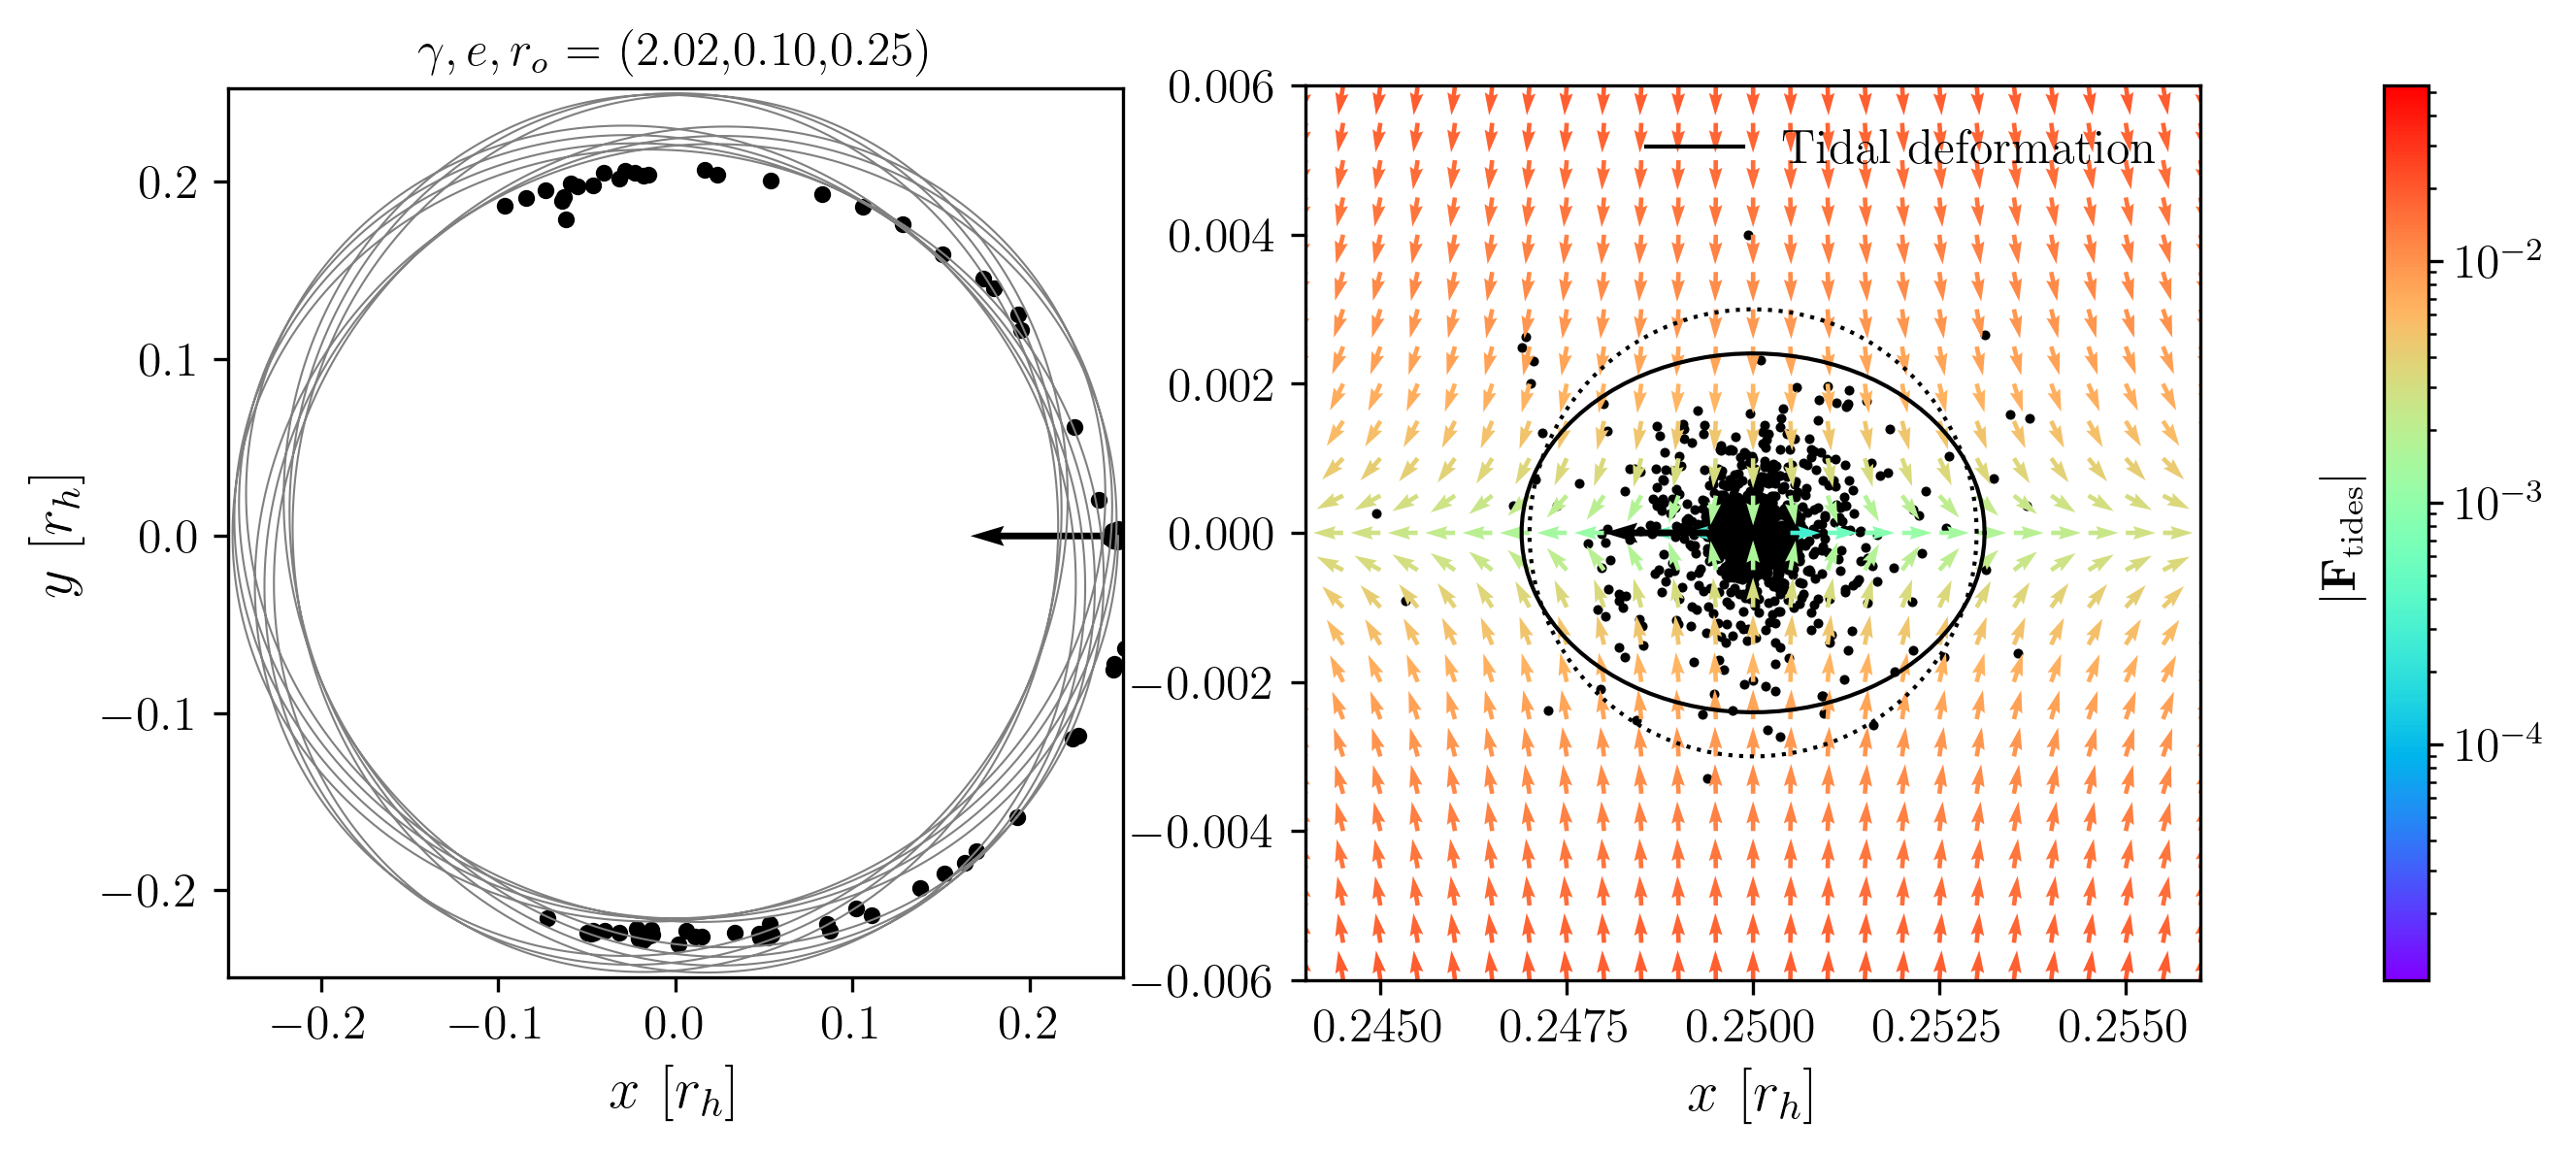
\includegraphics[width=\linewidth]{images/martos_tidal_field_202_10_25.png}
                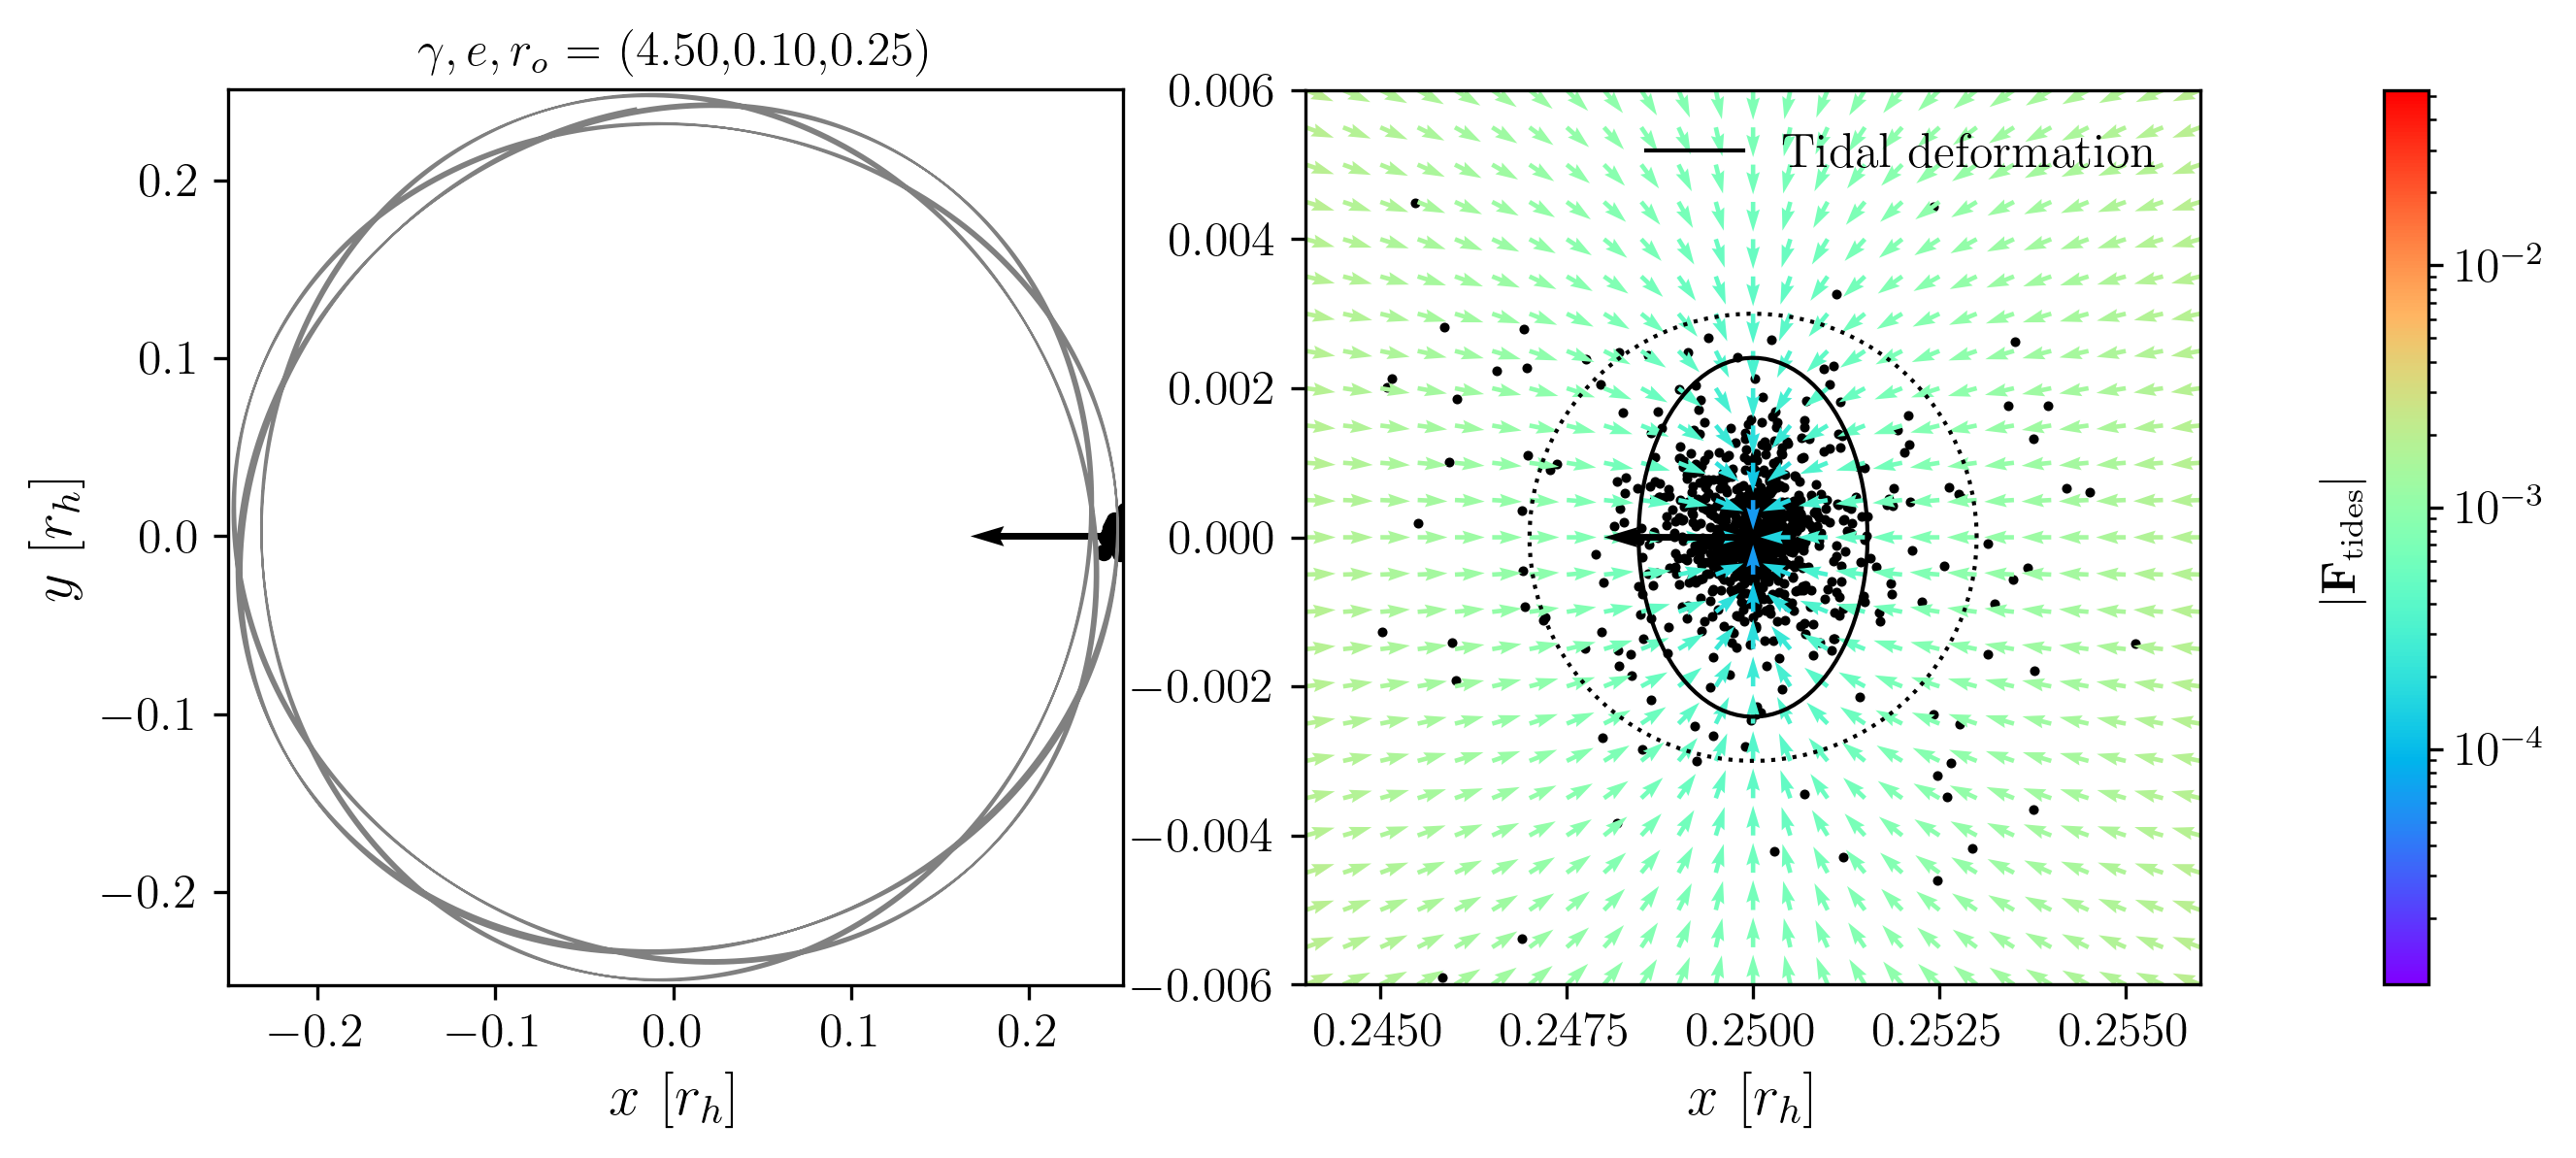
\includegraphics[width=\linewidth]{images/martos_tidal_field_450_10_25.png}
                \caption{The plots show two low-resolution streams (N = 1000) created by dissolving a Plummer sphere in the Martos halo potential. The units are scaled to the halo's characteristic radius. Gamma is the mass exponent and is the sole variable between the two simulations. The panels on the left show the orbit in gray and the stars in black. The black arrow points towards the center of the potential. The panels on the right show the tidal field, which is the tidal tensor evaluated at each position in space. The gray dotted circle is plotted with an arbitrary radius and is deformed by the tidal field into a black ellipse.}
                \label{fig:martos_tidal_field_small_r}
            \end{figure}

            \begin{figure}
                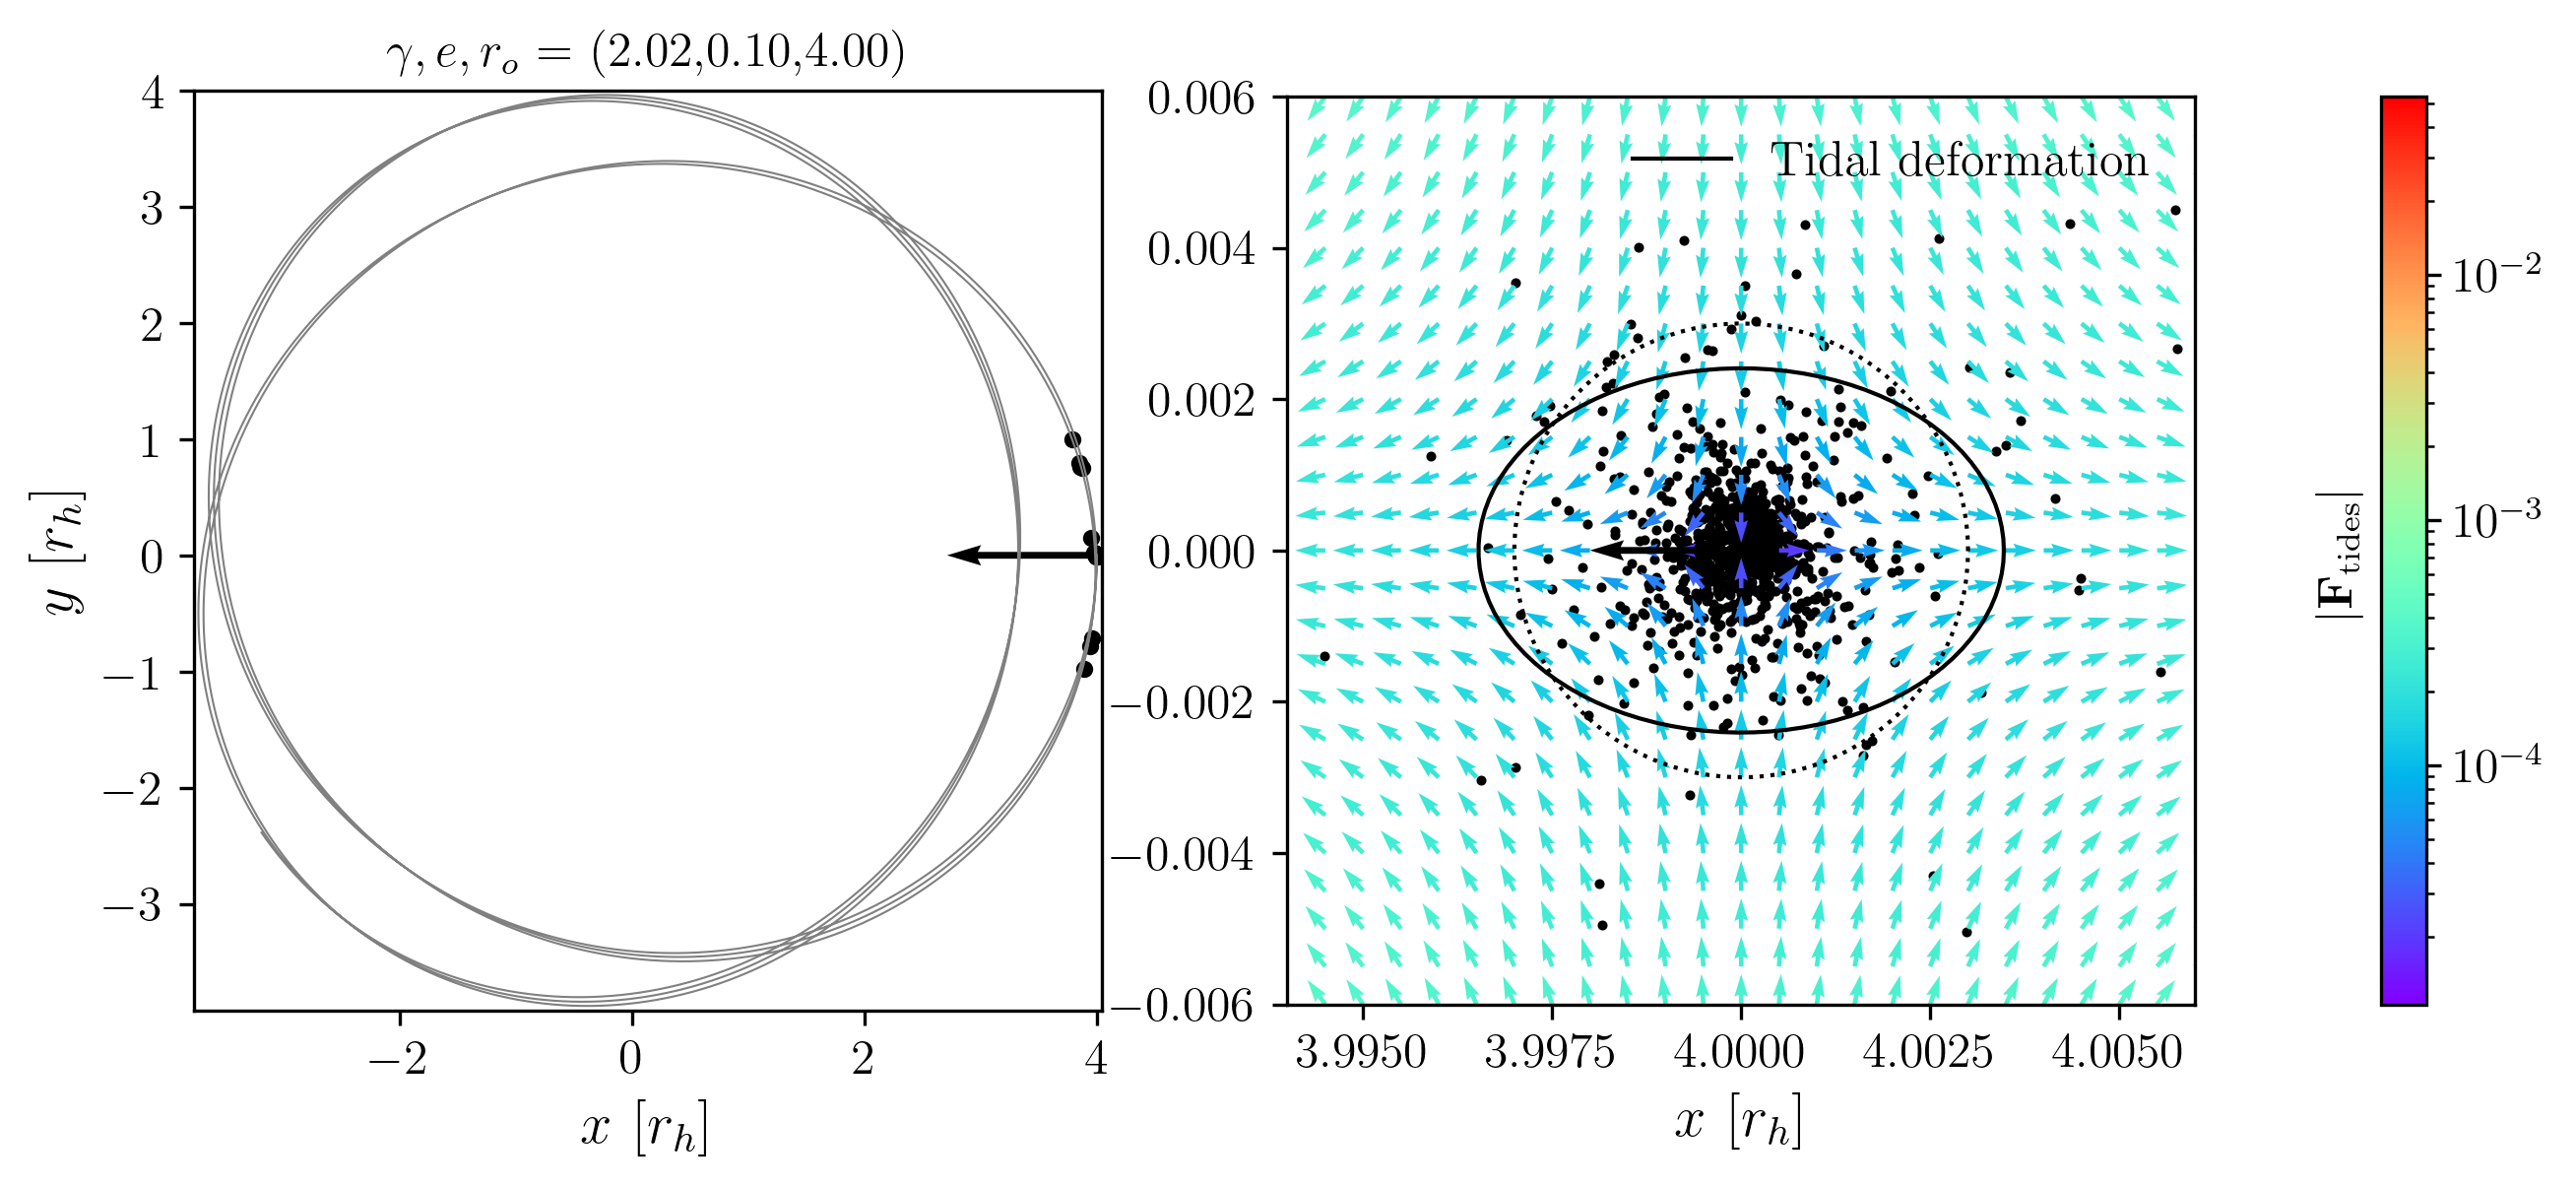
\includegraphics[width=\linewidth]{images/martos_tidal_field_202_10_400.png}
                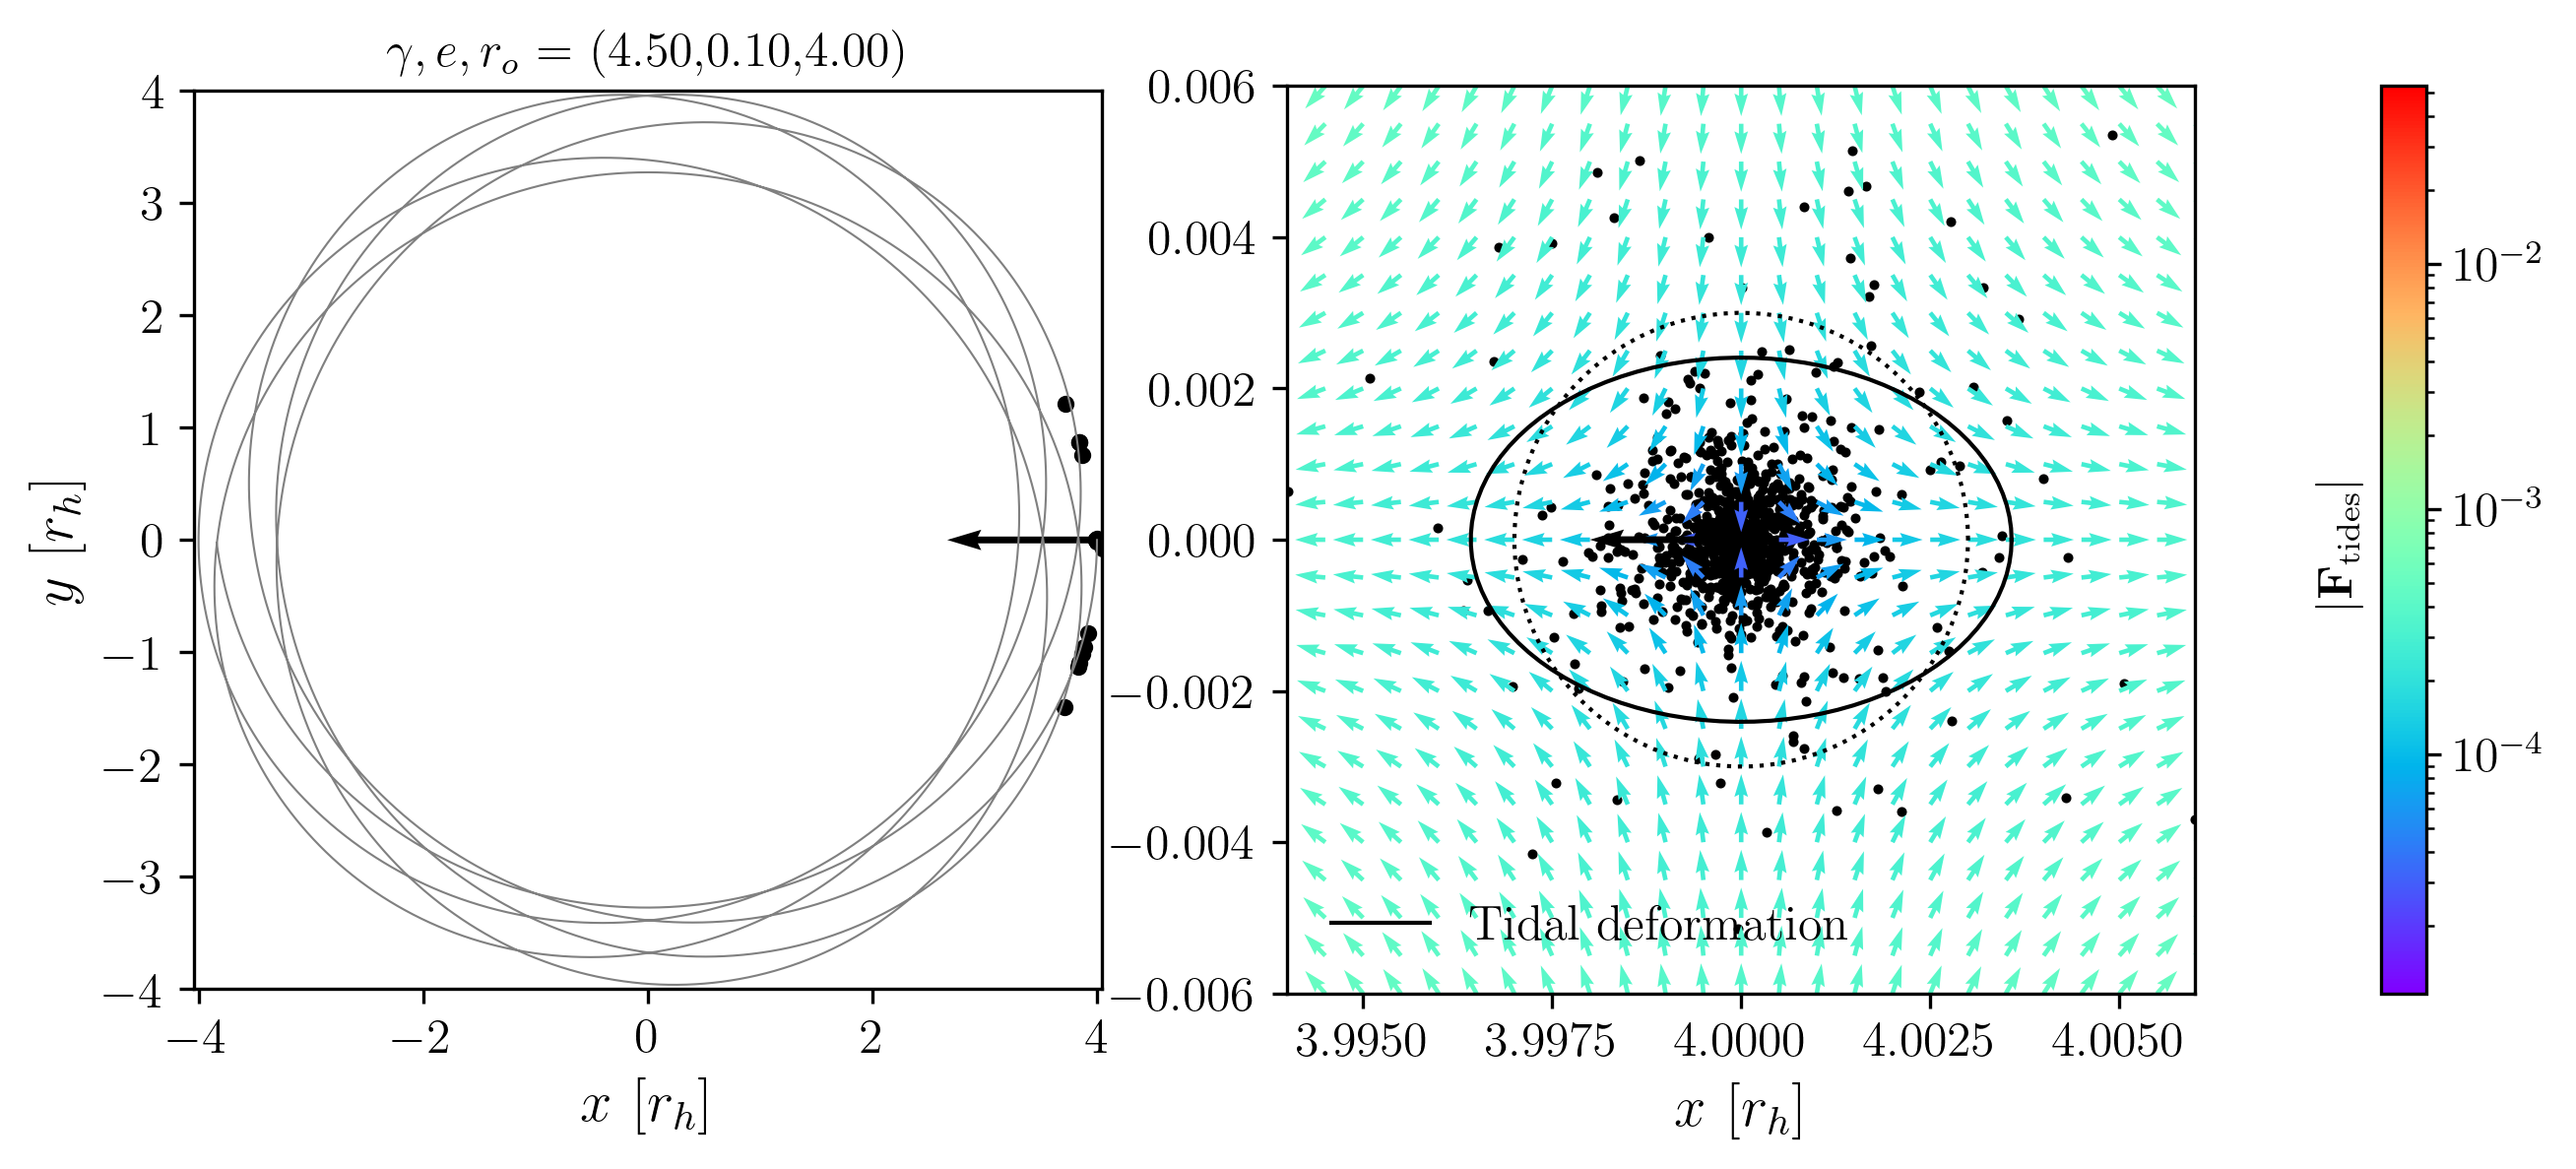
\includegraphics[width=\linewidth]{images/martos_tidal_field_450_10_400.png}
                \caption{The same experiment as Fig.~\ref{fig:martos_tidal_field_small_r}, but the cluster was placed at a larger distance of 4 $r_\textrm{halo}$, since we are beyond the characteristic radius, the tidal fields are the same, despite the different exponents $\gamma$.}
                \label{fig:martos_tidal_field_big_r}
            \end{figure}

            In the case of Fig.~\ref{fig:martos_tidal_field_big_r}, the tidal field returns to the typical situation where one axis is compressive and the other stretches. Notice how the deformations are similar in magnitude, while in the case of $\gamma=2.02$ for the top panel of Fig.~\ref{fig:martos_tidal_field_small_r}, the compression is stronger than the expansion. Both of these are different than the keplerian tidal deformation where the stronger deformation is stretching and whose axis is parallel to the position vector. 

    \subsection{The Distribution of Escaped Stars}
        Tidal forces cause stars to escape from the Lagrange points of the globular cluster. As we've seen, these forces can be compressive—pushing stars toward the cluster—or stretching—pulling them away, and specifically toward the Lagrange points. The stretching component is significantly amplified during pericenter passages, causing many stars to escape in bursts.

        This process doesn't fling stars into intergalactic space. Rather, the galactic tidal field is typically weak compared to the cluster's own gravitational pull, and escaping stars gain just enough energy to leave the cluster. As a result, they are still on very similar orbits to the clusters once they escape.

        But once stars escape, why do they form coherent stellar streams? And do they do anything else? To answer this, I must first introduce the concept of \textit{phase mixing}. This naturally leads us to discuss the range of possible orbits a globular cluster can follow, given observational uncertainties. I'll cover this fully before returning to the topic of stellar streams, which will be much easier to understand once this groundwork is in place.
        
        \textit{Phase mixing} is a direct consequence of Liouville's theorem, which follows from the collisionless Boltzmann equation. Liouville's theorem states that the infinitesimal volume element in phase space, \( d\mathbf{p}\,d\mathbf{q} \), is preserved under Hamiltonian evolution. In other words, the phase-space density \( f(\mathbf{q}, \mathbf{p}, t) \) remains constant along a particle's trajectory.

        To visualize this, instead of considering a single infinitesimal element, imagine a small cloud of initial conditions centered around \((\mathbf{q}_0, \mathbf{p}_0)\), with spread \(\sigma_q\) and \(\sigma_p\). While the total 6D volume of this cloud, \(\sigma_q^3 \sigma_p^3\), remains constant, differences in momentum cause the particles to move through phase space at different rates. Particles with higher momenta advance more quickly, while those with lower momenta lag behind. This leads to the cloud stretching and dispersing, even as its total volume is conserved. Since solutions to Hamilton's equations are unique, this dispersion reflects how nearby trajectories gradually diverge and spread over the available phase space—a process we call phase mixing.

        We can estimate the timescale for this spreading by considering how long it takes for orbits with slightly different energies to drift apart in phase. For example, in a Keplerian potential, the orbital period is given by
        \begin{equation}
            T^2 = \frac{4\pi^2 a^3}{GM},
        \end{equation}
        which depends on the semi-major axis, and thus on energy. In general, orbits in non-Keplerian potentials are not closed; particles precess and eventually fill out invariant tori in phase space. A characteristic timescale for this process can be estimated by dimensional analysis as
        \begin{equation}
            T_\mathrm{char} = C \frac{GM}{E^{3/2}},
        \end{equation}
        where \(C\) is a constant and \(E\) is the specific orbital energy.


        Consider now two nearby particles with energies $E - \Delta E$ and $ E + \Delta E $. Their orbital frequencies differ by:
        \begin{equation}
            \Delta f = \frac{1}{T( E - \Delta E)} - \frac{1}{T(E + \Delta E)}.
        \end{equation}
        The time required for the faster particle to lap the slower one in phase is the \textit{phase mixing time}, which is the inverse of the difference $2\pi / \Delta f$ and is given by:

        \begin{equation}
            T_\mathrm{mix} = \frac{2\pi}{\Delta f} = \frac{2\pi T_1 T_2}{T_2 - T_1}.
        \end{equation}

        For small energy differences \( \Delta E << E \), we can expand the period in a Taylor series to first order. This leads to:

        \begin{equation}
            T_\mathrm{mix} \approx T_\mathrm{char} \cdot 2\pi \left( \frac{E}{3 \Delta E} \right),
            \label{EQ:phase_mixing}
        \end{equation}
        Thus, the phase mixing time grows inversely with the relative energy spread in the population.

        \subsubsection{Orbital drift}
            The first manifestation of phase mixing is the growth of uncertainty in orbital solutions for globular clusters over time. This originates from the initial spread in orbital energies caused by observational uncertainties. In Fig.\ref{fig:phase_mixing_palomar_5_orbital_solutions}, I present an example based on Palomar~5, for which I compute 50 orbital solutions in our potential model. These initial conditions are sampled according to the uncertainties reported in the Baumgardt catalog. The figure shows that while the orbital solutions remain broadly similar, the lower-energy orbits progress through phase space more rapidly. In the bottom panel, the rightmost side includes overplotted dots indicating the final $(t, z)$ coordinates of each solution, illustrating that they span nearly the full range of $z$ values allowed by the initial conditions. In essence, once the integration time exceeds the phase-mixing timescale, any individual solution becomes speculative: the system could plausibly occupy any location in phase space permitted by the initial conditions.


            \begin{figure}
                \centering
                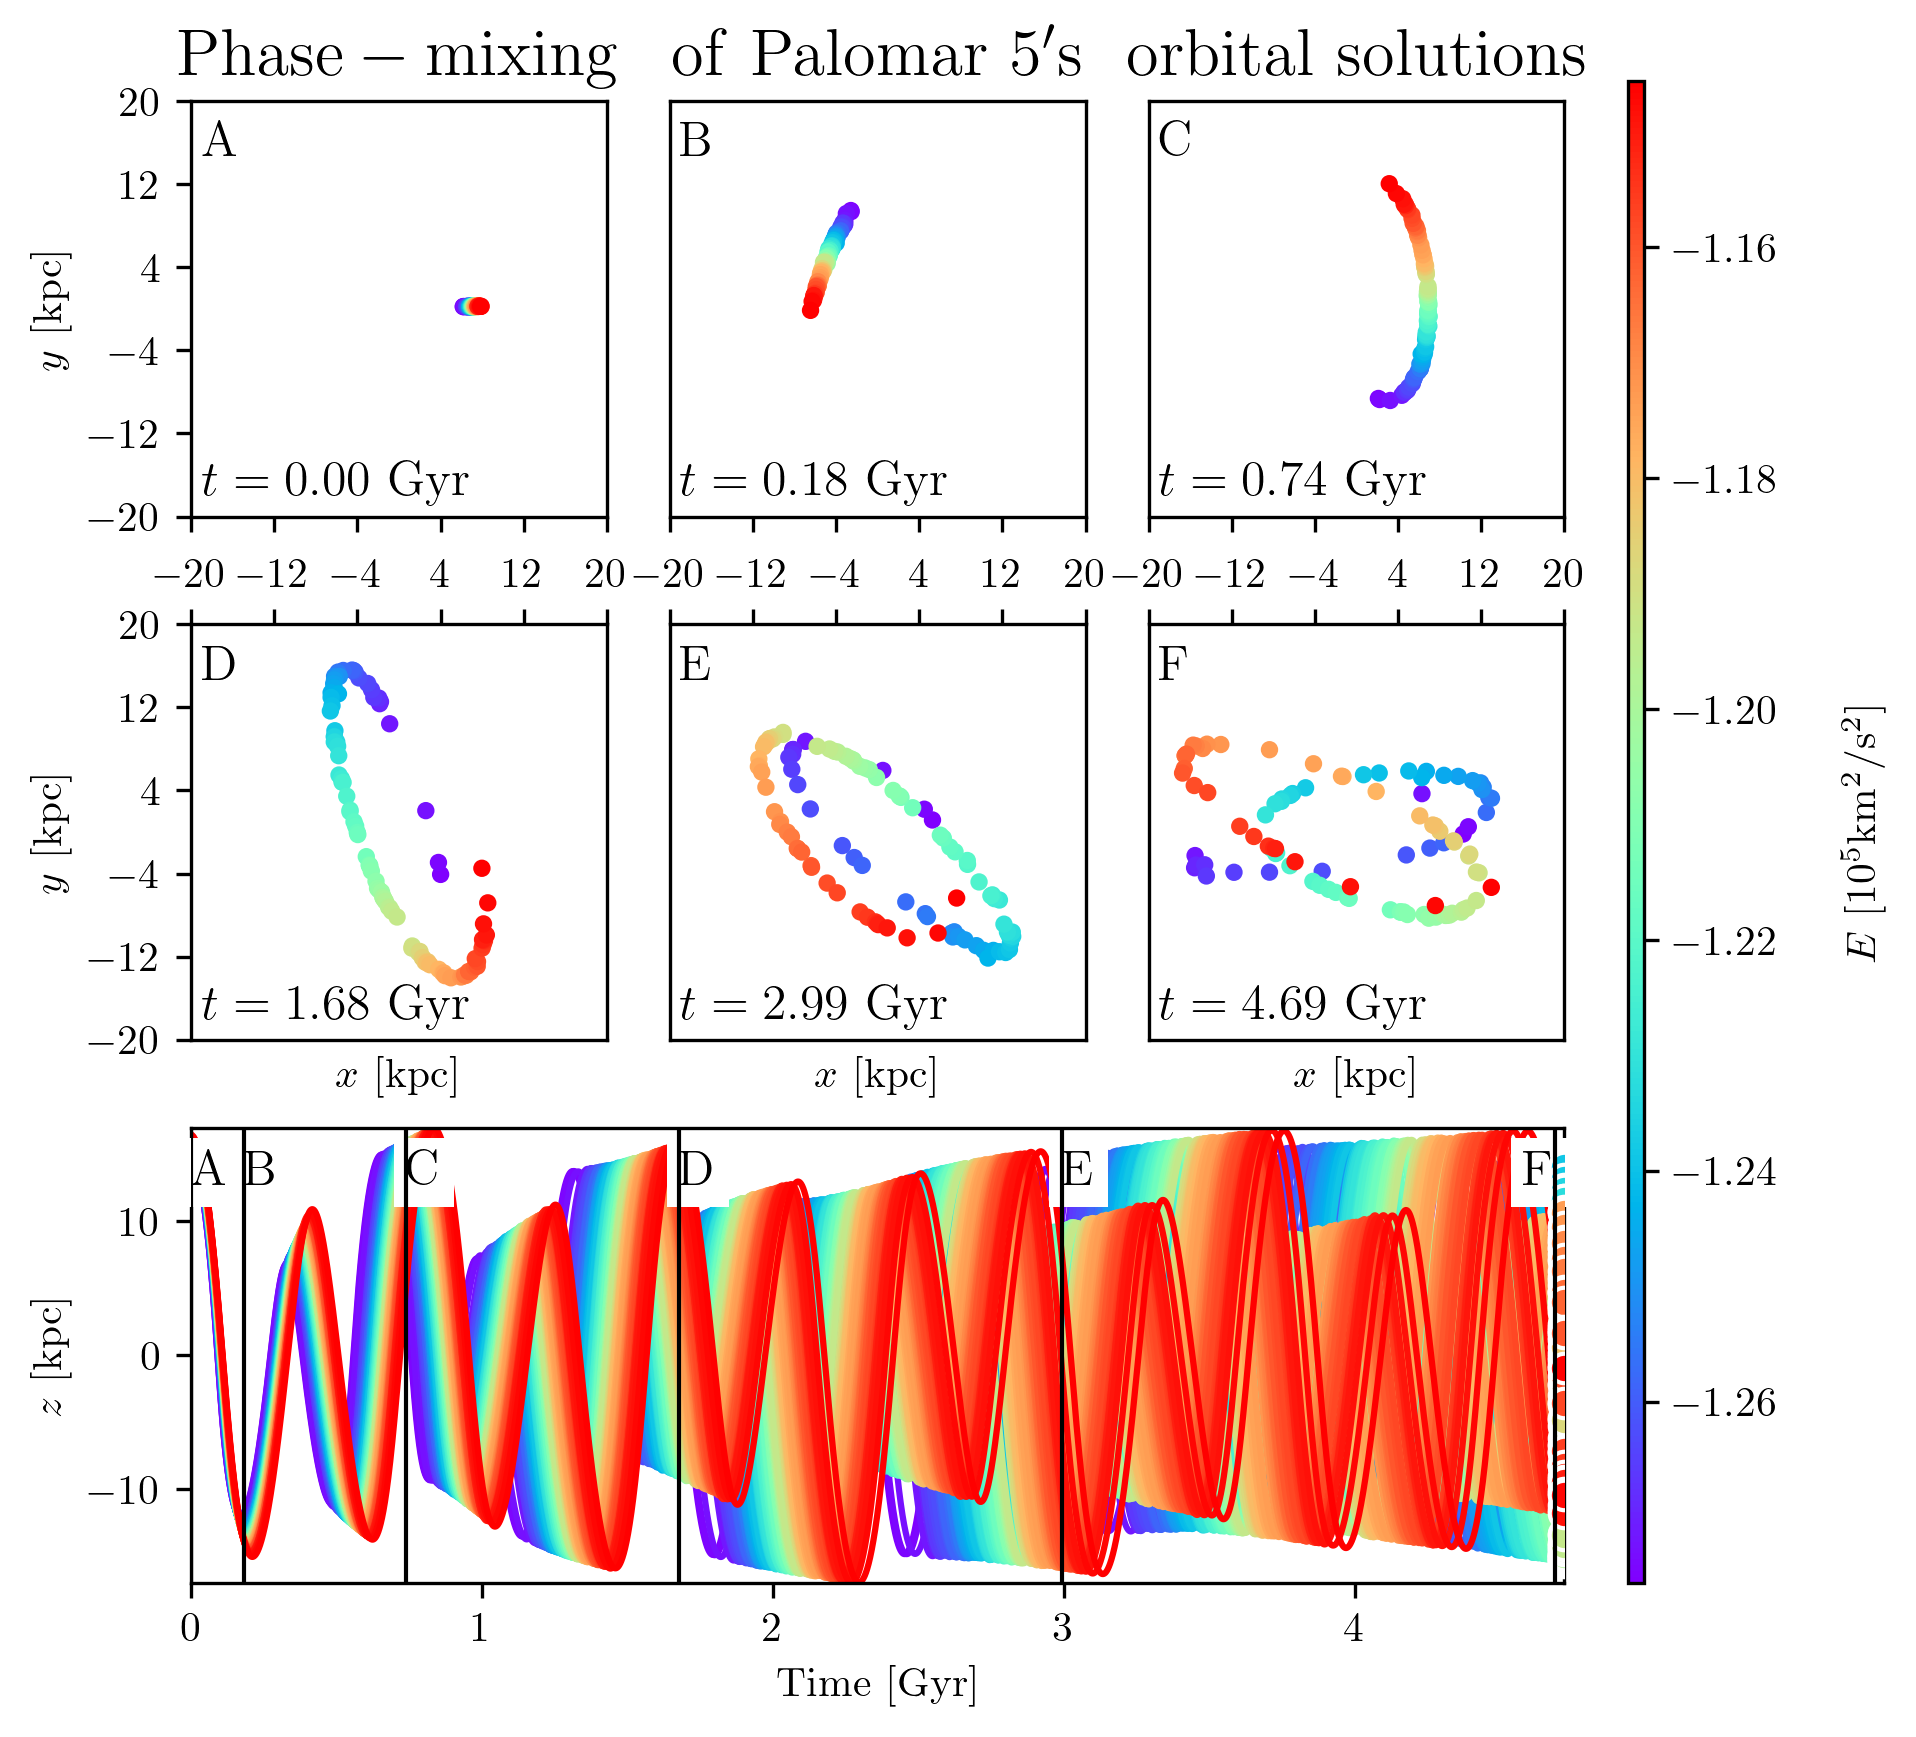
\includegraphics[width=\linewidth]{images/phase_mixing_palomar_5_orbital_solutions.png}
                \caption{Phase mixing of Palomar~5's orbital solutions in the \texttt{Pouliasis2017pii} potential. We sample 50 different initial conditions based on the observational uncertainties in distance, radial velocity, and proper motions. Each orbital solution is color-coded by its initial total orbital energy $E$. The top six panels show snapshots of the positions in the $xy$-plane of the orbital solutions at different times. The bottom panel shows the evolution of the $z$ coordinate as a function of time. Black vertical bars mark the timestamps corresponding to the snapshots in the top panels, which are labeled with matching alphabetical identifiers.}
                \label{fig:phase_mixing_palomar_5_orbital_solutions}
            \end{figure}    

            By inspecting Eq.\ref{EQ:phase_mixing}, we note that if the phase-mixing time is normalized by the characteristic orbital time, the resulting dimensionless mixing time is inversely proportional to the uncertainty in orbital energy. This relationship is general and holds for all orbits, regardless of their periods. However, it is still illustrative to examine this behavior in the context of the globular cluster catalog. In Fig.\ref{fig:phase_mixing_orbital_errors_sample}, I present the phase-mixing times for all Galactic globular clusters, based on current uncertainties from the Gaia DR3 catalog. The top panel shows the distribution for all 165 clusters. The bottom panels highlight the mixing behavior in cylindrical radius for a selection of statistically representative clusters: Gran~1, which has the shortest mixing time; Gran~5, the median case; NGC~6752, whose mixing time is closest to the mean; and NGC~2419, which has the longest mixing time.

            It is important to emphasize that these estimates are highly model-dependent. In some cases, the models predict phase-mixing timescales exceeding the age of the Universe. Unsurprisingly, the phase-mixing time correlates with the orbital period, which itself is related to the cluster's distance from the Galactic center. At large Galactocentric distances, the gravitational potential of the Milky Way becomes increasingly uncertain, as observational constraints on the Galactic mass distribution are weaker--See Fig.~\ref{fig:vasiliev_2021_EDR3_GCS_FIG_10} \citep{2021MNRAS.505.5978V}. Therefore, these extreme mixing times should not be interpreted as implying that we can predict the phase-space location of certain clusters with high confidence over cosmological timescales. 



            \begin{figure}
                \centering
                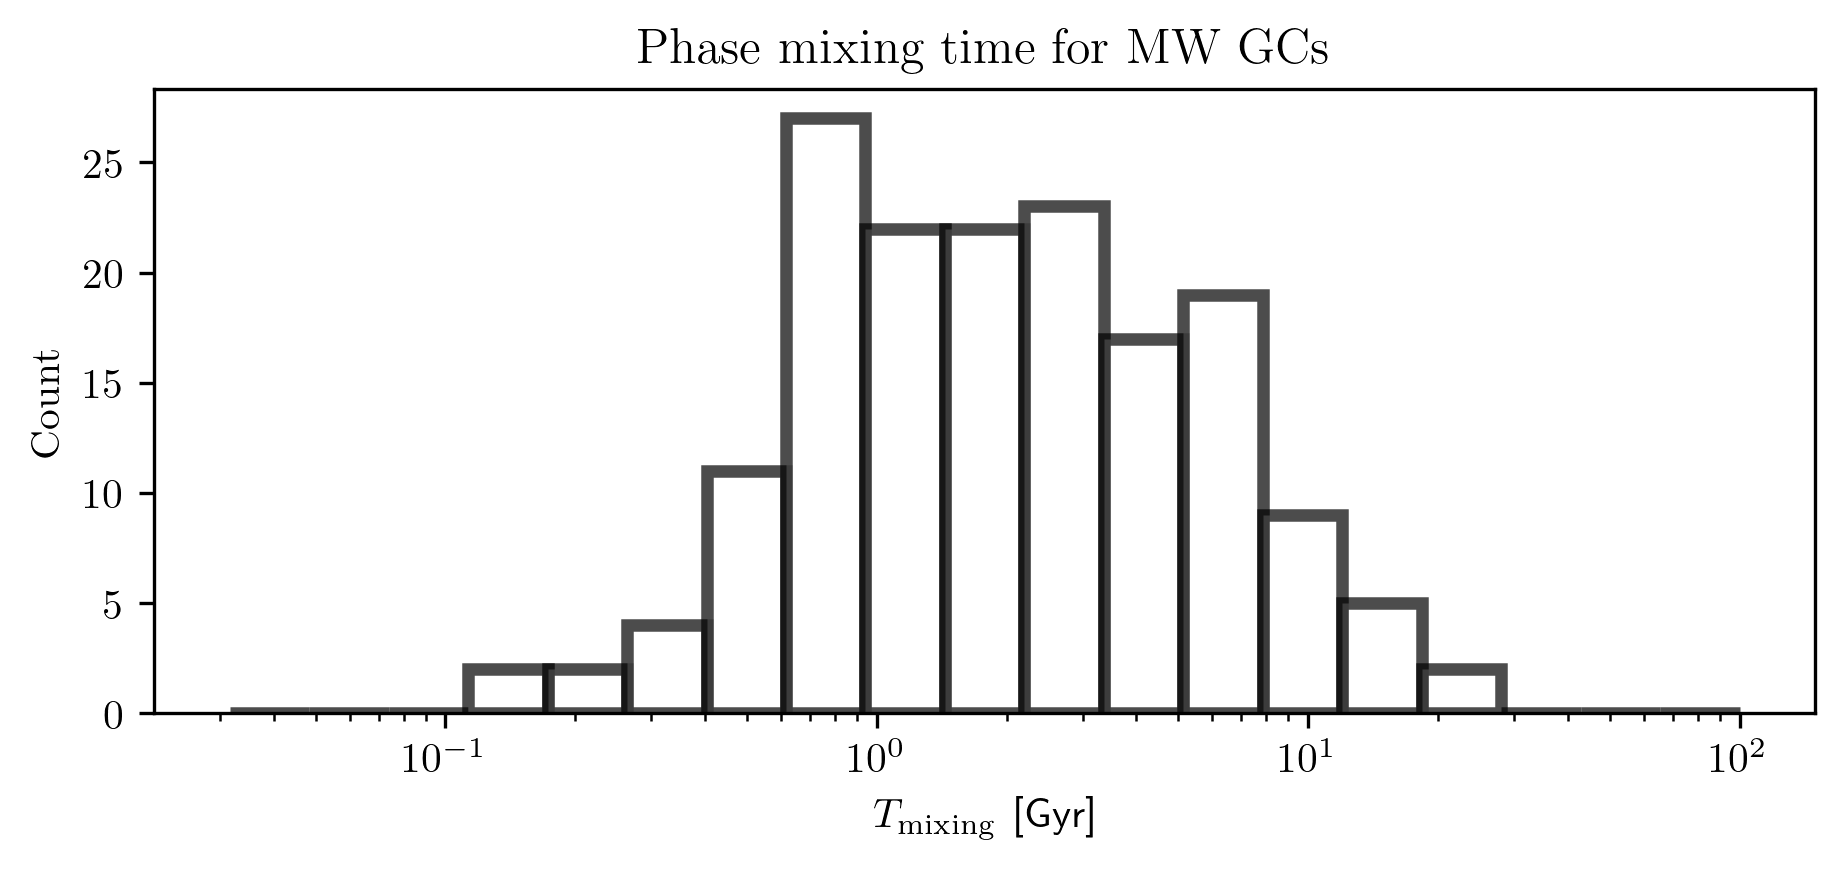
\includegraphics[width=.75\linewidth]{images/phase_mixing_time_histogram_MWGCS.png}
                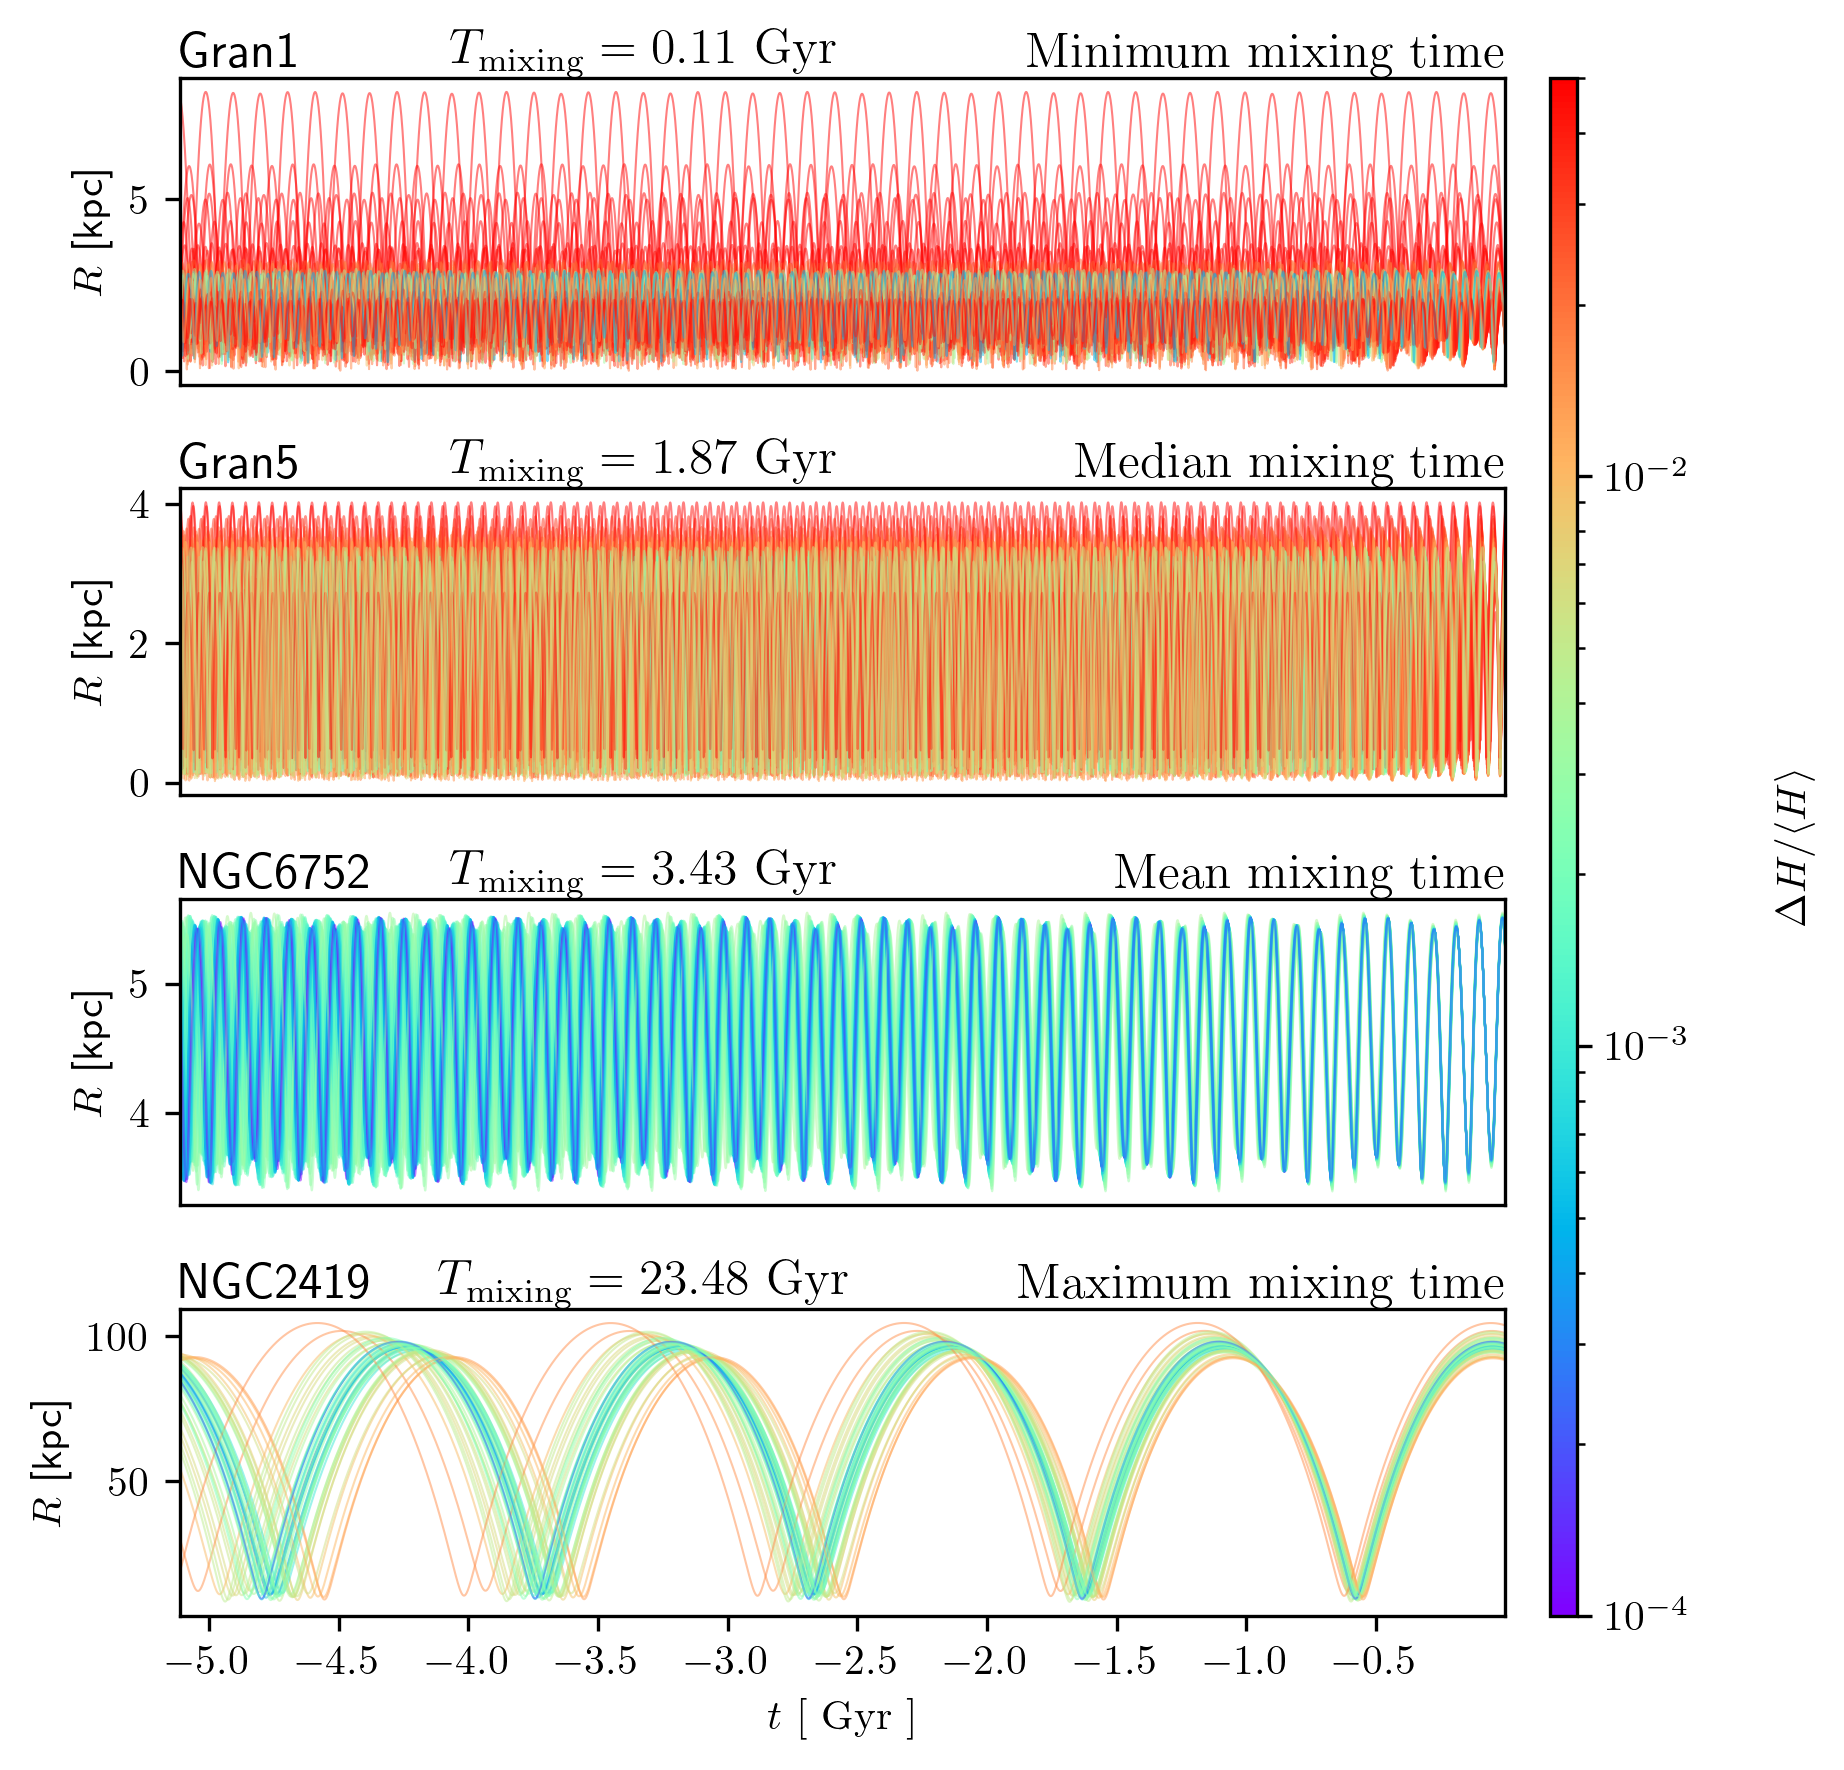
\includegraphics[width=\linewidth]{images/phase_mixing_orbital_errors_sample.png}
                \caption{The top panel shows the distribution of phase-mixing times for globular clusters, computed using Eq.~\ref{EQ:phase_mixing}. The following four rows illustrate the phase-mixing behavior for four selected clusters over the time range considered in this experiment. Orbital solutions are color-coded by their normalized deviation from the mean orbital energy.}
                \label{fig:phase_mixing_orbital_errors_sample}
            \end{figure}
     
            It's also interesting to note how the uncertainties in the orbital energy relates to the uncertainties in each observable. In Fig.~\ref{fig:energy_sensitivity_analysis_MWGCS_to_distance_RV_mu}, I perform this quick calulation. The uncertainties are measured in Galactic coordinates the ICRS coordinate system. This is a direct transformation to Galactic coordinates and thus can be expressed analytically.

            \begin{figure}[p]
                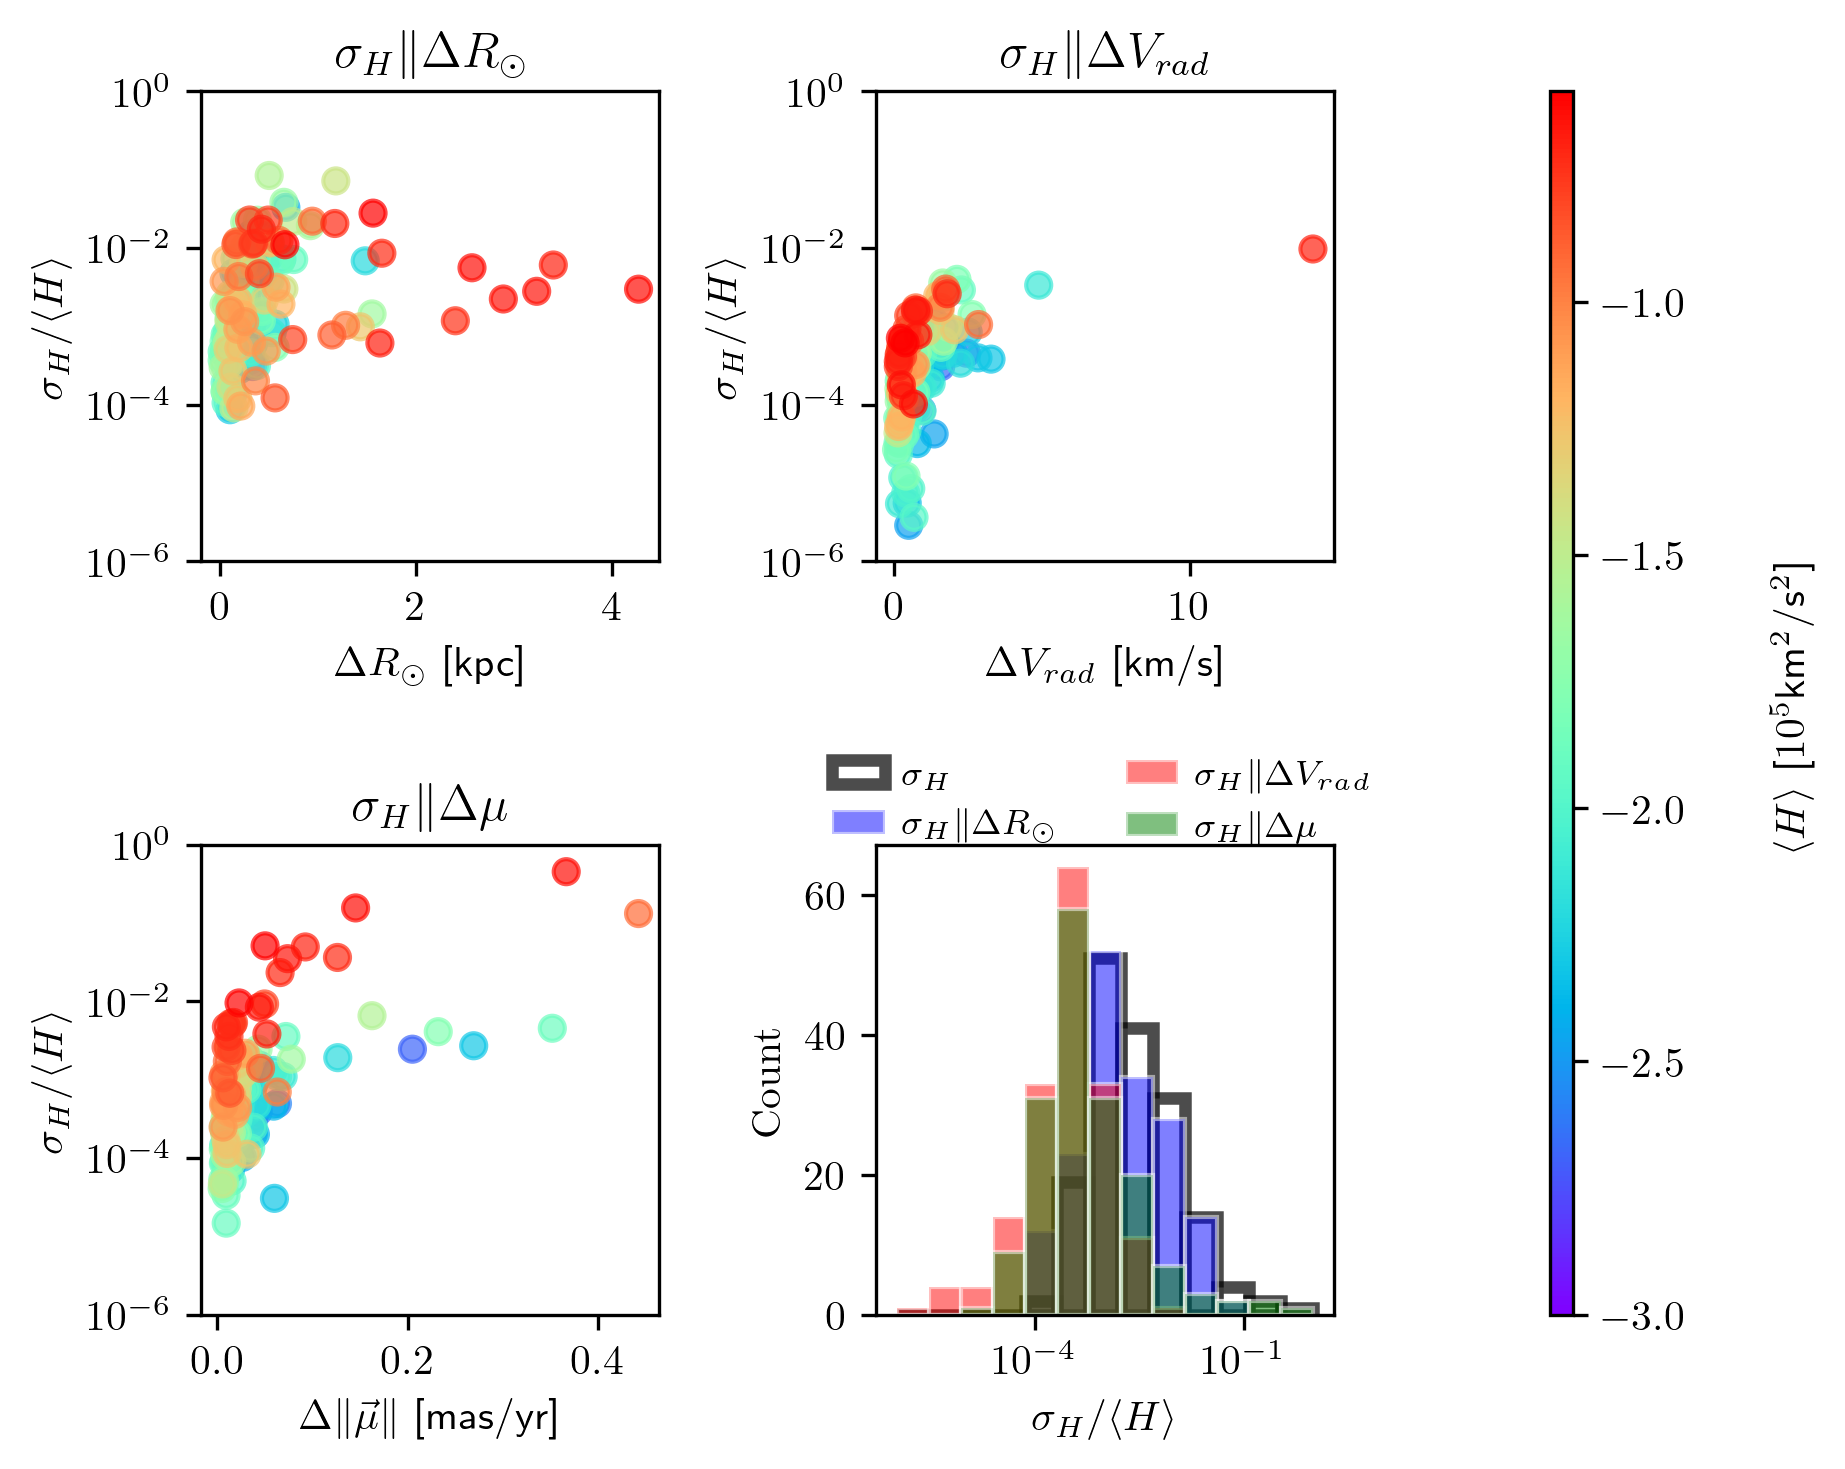
\includegraphics[width=\linewidth]{images/energy_sensitivity_analysis_MWGCS_to_errors.png}
                \caption{An analysis on the spread in orbital energies of the globular cluster population for each of its reported uncertainties. Each panel finds the STD in the Hamiltonain given the uncertainties in the specific variable. So the top left allows the distances to vary but holds the proper motions and radial velocities constant. It is plotted against the distance. The clusters are color-coated by their mean energies.}
                \label{fig:energy_sensitivity_analysis_MWGCS_to_distance_RV_mu}
            \end{figure}

            In short, the phase-mixing time for a given set of orbital solutions and the uncertainty in the initial conditions can be interpreted as: ``how long until I have no idea where this cluster is?'' Beyond this timescale, the cluster's position has an equal probability of being anywhere in phase-space permitted by its integrals of motion. This concept will be important in Chapter~5, where we assess whether different possible orbits for the globular clusters could have brought them into contact with the Palomar~5 stream.

        \subsubsection{Mixing of tidal debris}

            A cloud of points together in phase-space that are initially tightly packed together and then subsequently drift apart from one another, is a great analogy for the evolution of stars that escape from globular clusters to subsequently create stellar streams. For instance, at first glance, Fig.~\ref{fig:phase_mixing_palomar_5_orbital_solutions} might give the impression that we are looking at snapshots of a single stellar stream at different times. In reality, the figure shows different orbital solutions. This visual similarity underscores that both phenomena—stellar streams and diverging orbital solutions—are manifestations of phase mixing. 
            
            However, there is an important distinction. The divergence of different orbital solutions is an exact instantiation of the Louiville theorem. The particles have no influence on one another and they are all independently orbiting within the gravitational field. For stars within a globular cluster, the analogy breaks down because globular clusters are self-gravitating systems: stars interact gravitationally and remain bound for a significant time. This self-gravity slows down the mixing process. The time it takes for a globular cluster to dissolve and distribute its stars uniformly in phase space is typically longer than the idealized mixing time given by Eq.~\ref{EQ:phase_mixing}. Nevertheless, phase mixing still governs the long-term behavior of tidally escaped stars.

            Importantly, we need not consider all particles within the cluster to characterize the distribution of tidal debris as phase mixing. For clusters with short orbital mixing times compared to the simulation duration, stars that escape during the simulation can redistribute throughout the available phase space. While the resulting debris will not be uniformly distributed—an overdensity will remain at the cluster location—the tidal debris will broadly fill the phase space accessible to it. This point is crucial for the results discussed in Chapter 4.

            In fact, this can be seen in another \citet{2024ApJ...976...54P}. \citet{2024ApJ...976...54P} noted that today, there are roughly 170 known globular clusters. However, since they dissolve, there could have been many more. Thus, there could be many streams in the galaxy that are from now defunct globular clusters. Already, there are many known streams that are unassociated to globular clusters \citep{2022ApJ...926..107M}. In fact, of the roughly 90 known stellar streams, only about 20 are associated to globular clusters \citep{2024ApJ...967...89I}. \citet{Pearson et al. (2024)} set out to predict the the total number of stellar streams we can expect in a Milky Way like Galaxy from IllustrusTNG \textbf{get ref}, by using inserting prescription of globular cluster formation and distribution within the Milky-Way analog as well as those that were imported by eaten dwarf galaxies following the methods of \citet{2022MNRAS.514.4736C,2023MNRAS.522.5638C}. \citet{Pearson et al. (2024)} simulates the dissolution of these hypothetical globular clusters adn studies the resultant tidal debris. A panorama of this is presented in Fig.~\ref{fig:perason-2024-fig}. 

            \begin{figure}
                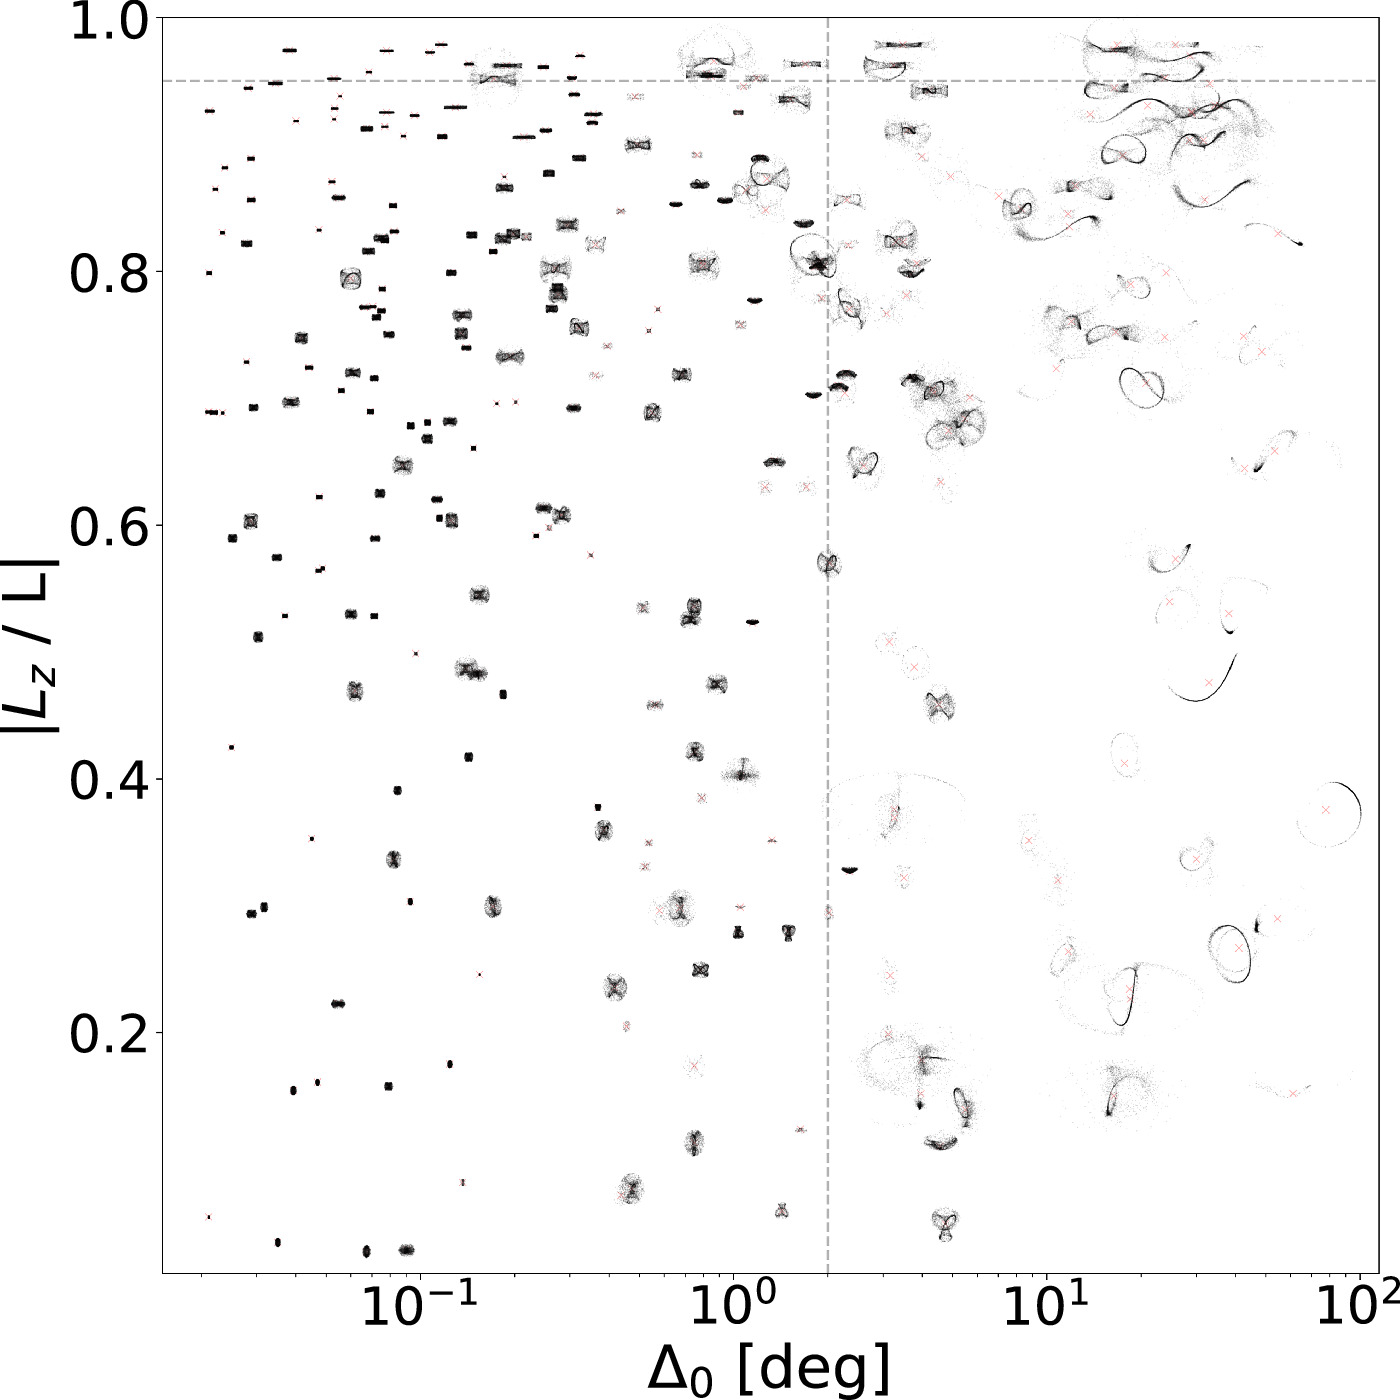
\includegraphics[width=\linewidth]{images/perason-2024-fig.jpg}
                \caption{A catalog of expected debris of a simulated totally disrupted population of globular clusters within a Milky Way analog. The y-axis is the normalized z-component of the angular momentum, with zero corresponding to polar orbits and 1 corresponding to planar orbits. The x-axis is a ``distance'' of the ``center-of-mass'' of a stream from the galactic center. Each stream is plotted in galactic coordinates annd are to scale with one-another. The bottom right quandrant satisfies their ``streaminess criterion''. Credit: Fig~7 of  \citet{2024ApJ...976...54P}.}
                \label{fig:perason-2024-fig}
            \end{figure}

            \citet{2024ApJ...976...54P} created a ``streaminess'' criterion. They base this on two metrics. The first, is the distance from the ``center-of-mass'' of a stream from the galactic-center in galactic coordinates. This metric is:
            $\Delta_0 = \sqrt{\mathrm{medn}(b)^2+\mathrm{medn}(l)^2}$. The argument being that is this number is close to zero, then the tidal debris is symmetrically distributed about the center of the galaxy and fully phase-mixed. 

            \citet{2024ApJ...976...54P} results are promissing and note that the current catalog of stellar streams is very incomplete and we could expect up to 1000 stellar streams within the Milky Way. I would like to note, that for even for totally phase mixed tidal debris, it is finds co-moving groups \citep{2018MNRAS.477.4063M,2018MNRAS.478.3862M}. While the totally phase-mixed debris appears incoherrent, the stars are still moving along the same trajectory yet are offset by phase. For example, the stream \textit{Fimbulthul} has been associated to $\omega$~centauri (NGC~5139), the most massive cluster that is suspective of being the remnant of an accreted dwarf galaxy (\textbf{Majewski 2000}, \textbf{Johnson \& Pilachowski 2010}, \textbf{Bellini et al. 2018}). Our simulations in Chapter~4 predict that the debris from $\omega$~centauri are totally phase-mixed and would not be classified as \textit{streamy}. Nonetheless, \textit{Fimbulthul} perfectly aligns the near-future orbital trajecotry of $\omega$~centauri and is consistent with $N$~body predictions \citep{2021ApJ...914..123I}.

            \textbf{What about the } actions for classifying the streams? 

            
    \subsection{Massive objects colliding with stellar streams}
        
        Previous we described how they escape the globular clusters. Then we described how the escaped stars can redistribute themselves in the galaxy following a nice evolutionary flow in the gravitational field from normal hamiltonian evolution. However, other things can happen to the stream. Notably, other massive objects in the galactic field can fly-by and perturb the orbits of some of these stars. Here, I would ike to summarize this. 

        Collisions are essential in this thesis for two reasons. Firstly, one of the main research questions is how the passage of a subhalo perturbs a stellar stream. This interaction can be treated as a gravitational collision.

        In general, we are interested in how much the momentum of a particle changes before and after the encounter. We can simplify the scenario by assuming that the target particle is initially at rest, and that the perturber (the subhalo) flies by with a minimum distance of approach $b$—the \emph{impact parameter}.

        Since both objects exert gravitational forces on each other, the target will gain energy and begin to move, while the perturber will be slightly deflected and slow down. However, to simplify the calculation, we assume the perturber is unperturbed by the target—i.e., it moves on a straight-line trajectory with constant speed $v$.

        In this approximation, we compute the momentum change of the target by integrating the gravitational force over time. Gravity is always attractive: the perturber pulls the target particle to the left before the closest approach and to the right afterward. If the trajectory is symmetric and unperturbed, the components of the force parallel to the motion cancel out. Thus, the net momentum transfer is perpendicular to the motion of the perturber.

        Assume the perturber moves along the $x$-axis with impact parameter $b$, and the target lies at the origin. Then the net force acts in the $+y$ direction. The gravitational force scales as $1/d^2$, so for distances $d >> b$, the force becomes negligible. We can then approximate the force as roughly constant over a short time interval during the closest approach.

        We estimate the duration of the interaction as the time it takes the perturber to travel a distance $2b$ (from $x = -b$ to $x = +b$), giving $\Delta t = 2b/v$. Assuming a constant perpendicular force $F_\perp \approx GMm/b^2$, the change in momentum is:

        \begin{eqnarray}
        m\,\delta v_y &=& \int F_\perp \, dt \\
                    &\approx& F_\perp \cdot \Delta t \\
                    &=& \frac{GMm}{b^2} \cdot \frac{2b}{v}
        \end{eqnarray}

        Dividing both sides by $m$, the change in velocity is:
        \begin{equation}\label{eq:delta_v_impulse_approx}
        \delta v_y = \frac{2GM}{b v}
        \end{equation}

        It is interesting to note that this result is inversely proportional to the velocity of the perturber. This behavior contrasts with contact collisions, where a higher speed typically results in a greater momentum transfer. In gravitational encounters, a faster flyby leads to a shorter interaction time and thus less momentum exchange.

        \subsubsection{Gapology}
            Gaps in stellar streams are underdensities that appear after encounters with dark matter subhalos or globular clusters. These can be understood as resulting from collisions. However, modeling the interaction as one point mass hitting another is too simplistic. What happens when an extended object, like a subhalo, interacts with a continuous stellar stream? Before delving into the technical details, it is worth clarifying a misconception--one that I myself held when first approaching this problem. Encounters between stellar streams and perturbers are not violent collisions in which stars are physically ejected or stripped from the stream. Rather, the perturber imparts a small, localized change in velocity to nearby stars, subtly altering their orbital periods. Over time, these tiny shifts accumulate, causing stars to drift apart and gradually sculpting a visible underdensity: the gap. 
            
            To address this, we turn to the work of \citet{2015MNRAS.450.1136E}, who studied a simplified model: a stream with uniform density on a circular orbit. This idealized setup allows for an analytical treatment of the gap's formation and evolution. A gap can be characterized by two main quantities: its angular width, $\Delta \theta$, and the density contrast, $\rho_{\mathrm{peak}}/\rho_0$, between the overdensities at the gap's edges and the central underdensity.


            To understand how these evolve, the authors derived a parameterization of the change in velocity $\Delta \vec{v}$ for stars along the stream after a perturbation. This vector function depends on the position $y$ along the stream relative to the impact point and on several parameters describing the perturber and the impact geometry:
            \[
            \Delta \vec{v} = f(y \,|\, M, r_s, b, w_\parallel, w_\perp, \alpha),
            \]
            where $M$ is the impactor's mass, $r_s$ its scale radius, $b$ the impact parameter, $w_\parallel$ and $w_\perp$ the components of its velocity parallel and perpendicular to the stream, and $\alpha$ the angle between the impactor's trajectory and the $(x,z)$-axes.

            To set up the problem, a coordinate system is defined where the stream lies along the $y$-axis, and the impact occurs at $y=0$. Because the stream has spatial extent, the impactor's motion must be decomposed into parallel and perpendicular components with respect to the stream. Unlike the simpler point-mass approximation, here $\Delta \vec{v}$ generally has nonzero components in all directions. In particular, $\Delta v_y$ alters the speed along the stream, while $\Delta v_x$ and $\Delta v_z$ displace stars out of the stream's plane. $\Delta v_x$ or $\Delta v_z$ can be zero if the trajectory of the impactor is parallel to the $x$ axis or $z$ axis, respectively. 

            The expression for $\Delta v_y$ is:
            \[
            \Delta v_y\left(y\,|\, M, r_s, b, w_\parallel, w_\perp\right) = - \frac{2GM w_\perp^2 y}{w\left[\left(b^2 + r_s^2\right)w^2 + w_\perp^2 y^2\right]},
            \]
            which is an odd function of $y$, as expected for a gravitationally attractive force: stars ahead of the impact point ($y>0$) are slowed down, while those behind ($y<0$) are sped up.

            \begin{figure}
                \centering
                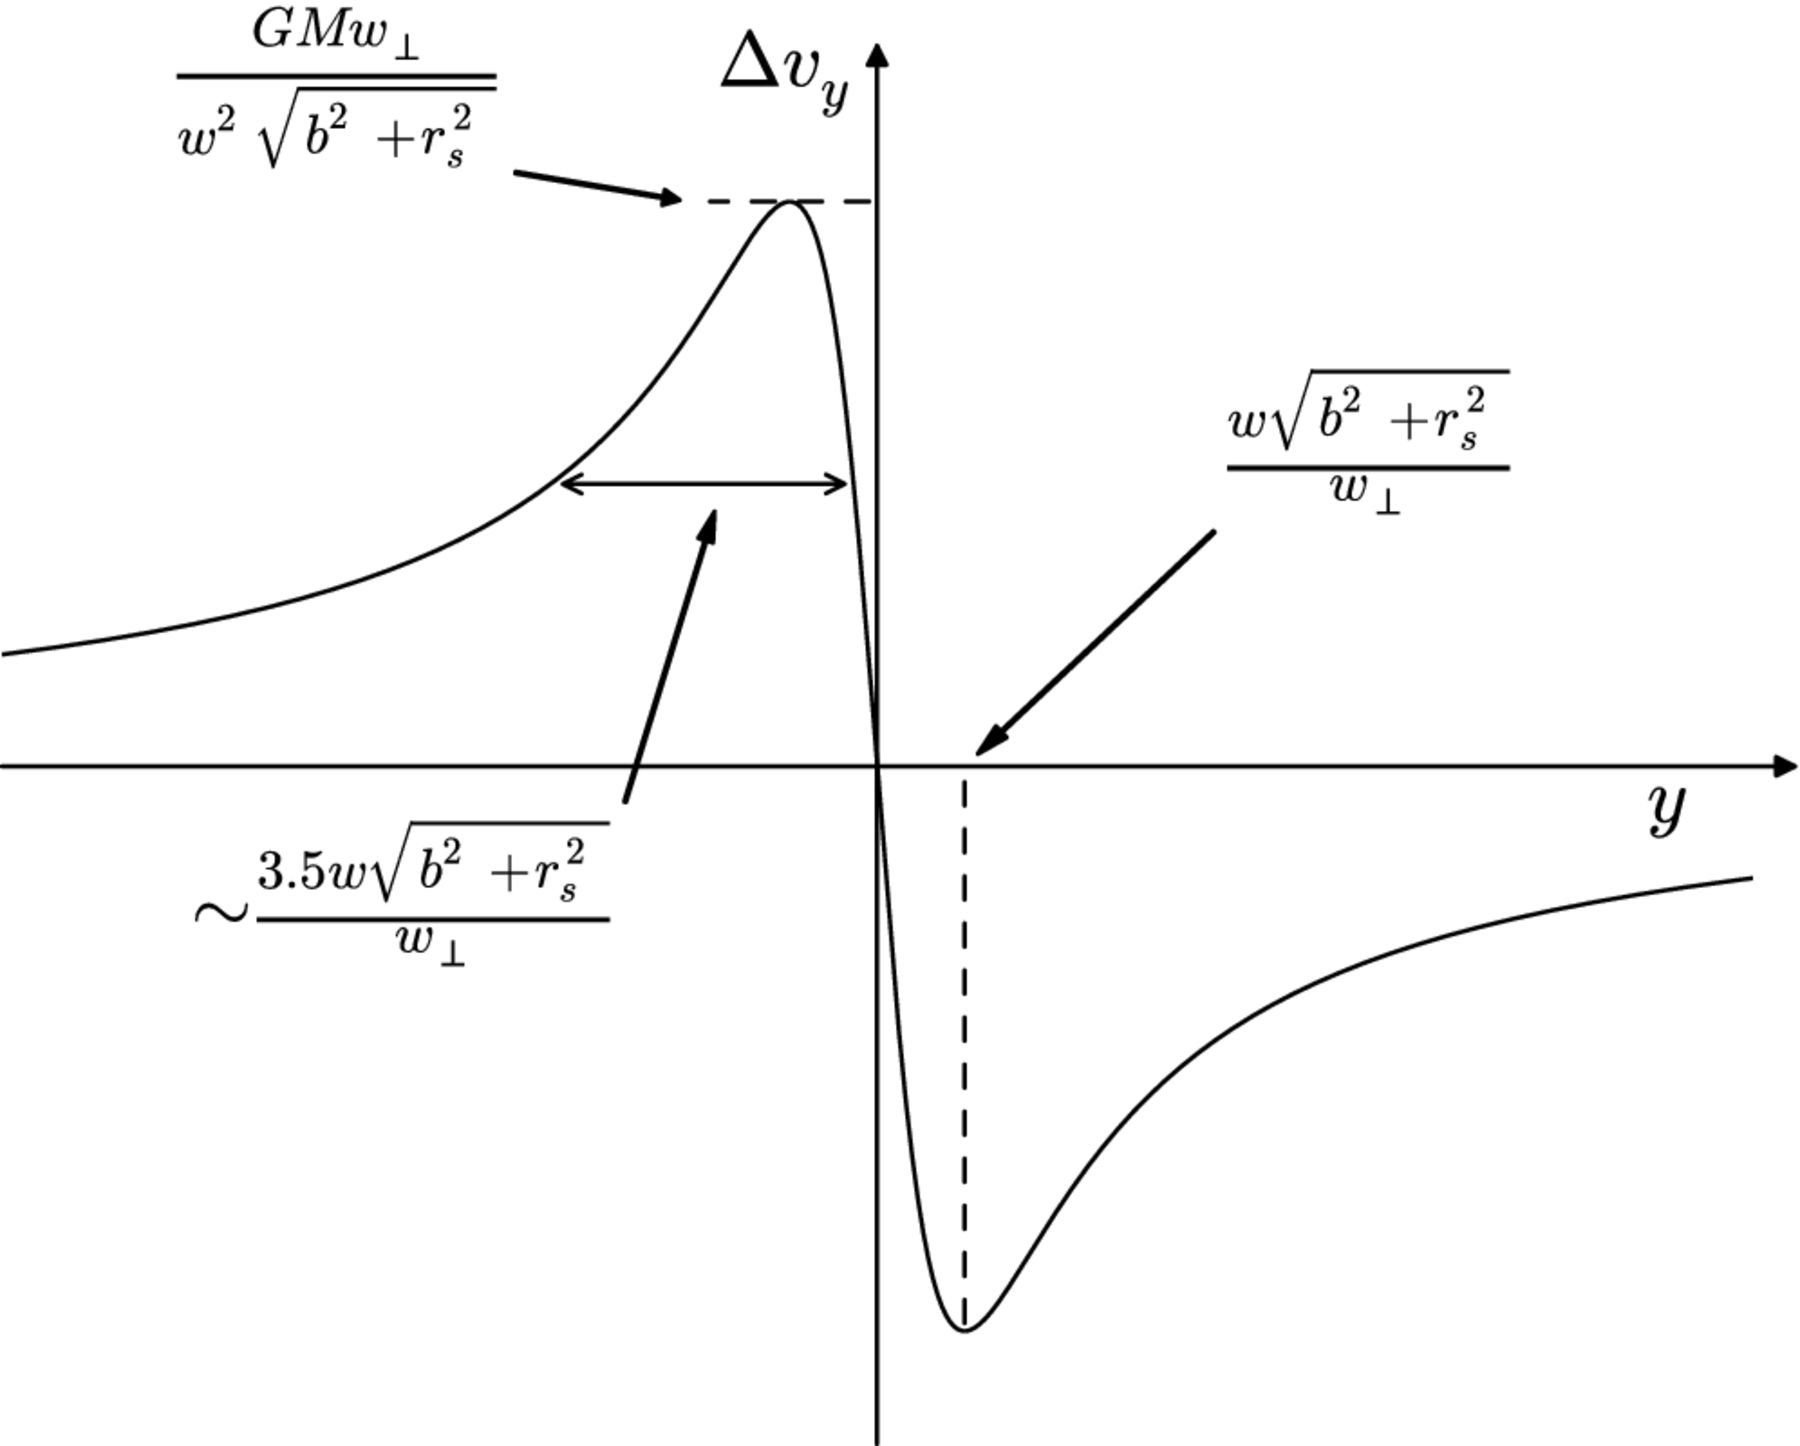
\includegraphics[width=\linewidth]{images/erkal_et_al_2015_fig_3.png}
                \caption{The change in velocity, $\Delta v_y$, of stars along the stream after an impact. The stream lies along the $y$-axis, with the point of impact at the origin. Key features are labeled: the maximum value of $\Delta v_y$, its location, and the full width at half maximum. Taken from Fig.~3 of \citet{2015MNRAS.450.1136E}.}
                \label{fig:erkal_2015_fig_3}
            \end{figure}

            Several assumptions underlie this formulation. First, the stream is approximated as a straight line, which requires the size of the impacted region to be much smaller than the orbital circumference. Second, the velocities of both the stream and the perturber are assumed constant, implying that the duration of the impact is much shorter than the system's orbital period. These assumptions also imply that the impactor must pass close to the stream and be compact relative to the stream's orbital radius.

            The authors then developed the time evolution of the stream's density following the impact. To study these, the authors employed three complementary approaches:
            \begin{enumerate}
                \item A numerical solution of a transcendental equation governing $\Delta \theta(t)$;
                \item A fully analytic solution for a low-order analytical approximation valid when the gap opening $\Delta \theta$ is still small;
                \item An $N$-body simulation of the full system.
            \end{enumerate}

            Together, these revealed three distinct phases of gap evolution:
            \begin{enumerate}
                \item \textbf{Compression phase} --  Shortly after the impact, stars on opposite sides swap places, briefly compressing the stream until the right and left sides overtake one another. 
                \item \textbf{Linear growth phase} -- The gap grows roughly linearly in time, as stars move apart under their velocity differences.
                \item \textbf{Caustic phase} -- Eventually, stars bunch up at different locations at the edges of the gap, creating sharp overdensity features (``caustics''). Additionally, the gap's growth to is slowed to a sublinear rate, scaling roughly as $\propto \sqrt{t}$.
            \end{enumerate}


            The author's make an important realization. Even in a scenario where the galactic potential and the stream's orbit are known, with just the gap's density profile there are still seven parameters that describe it's shape: $M,r_s,b,w_\perp,w_\parallel,\alpha,t$. The authors state that the gap's profile provide two more piece of information and with a constraint on the perturber's density, we would still be left with four degrees of freedom. The problem is thus underdetermined and it is thus impossible to uniquely determine the properties of the perturber. A large statistical sample of gaps would be required to constrain a population of dark matter subhalos. With the ever increasing data quality, perhaps this could be possible someday.  

            While powerful, the authors describe how the limiting assumptions impact the interpretations of this work. First, the framework is limited to circular orbits which poses a significant constraint especially for globular clusters which often have inclined and eccentric trajectories. Indeed, as they discussed in their work, streams do not have uniform densities. Stars that populate the streams come from tidally disrupting stellar systems. As they leave the cluster and enter the stream, they come with a range of energies and and angular momenta that in essence eliminate any casutic features. 

            \citet{2016MNRAS.457.3817S} expanded on this foundation and provided a truly exchaustive and comprehensive exploration of stream-subhalo interactions. Their primary methodological innovation was the development of a framework for modeling the impact of dark matter subhaloes on cold, thin streams in angle-frequency space. This space significantly simplifies stream dynamics, allowing for the rapid generation of general stream models and proving ideal for incorporating velocity perturbations from subhaloes. They developed methods to compute velocity, angle, and frequency kicks for general subhaloes and impact geometries, then translated these into angle and frequency perturbations. This framework allowed for an extensive range of experiments:

            \begin{itemize}
                \item \textbf{Various perturber models}: \citet{2016MNRAS.457.3817S} compared velocity kicks produced by various astrophysically relevant subhalo profiles, including Plummer, Hernquist, truncated Navarro-Frenk-White (NFW), and non-truncated NFW profiles. They found that while there are differences in kick amplitudes depending on the profile, the absolute differences between these methods were generally small, especially for lower-mass impacts, suggesting the simpler "curved approximation" (which accounts for stream curvature but assumes fixed relative velocity during flyby) is often sufficient
                \item \textbf{Different Orbits for the Progenitor}: key advancement was the focus on streams formed from progenitors on eccentric orbits. This directly addressed a limitation of \citet{2015MNRAS.450.1136E}, which primarily restricted its analysis to streams on circular orbits. The angle-frequency space formalism is particularly well-suited for modeling these more complex, realistic eccentric stream dynamics.
                \item \textbf{Different Impact Points}: The study thoroughly investigated how the stream changes depending on where along the stream the impact occurs. They simulated impacts both close to the progenitor (where particles are more mixed in energy) and further downstream (where particles are better ordered by energy), finding that the growth rate of the gap depends on the impact location. 
            \end{itemize}

            Drawing from these comprehensive investigations, \citet{2016MNRAS.457.3817S} reached several essential conclusions and insights into ``gapology'':
            \begin{itemize}
                \item \textbf{Dominance of Frequency Kicks}: They found that angle perturbations from a flyby are generally only significant on short timescales (less than a radial period). At later times, the frequency perturbations become much more important, controlling the future structure of the gap. These frequency perturbations are simply related to the velocity perturbations (specifically, the change in energy, $v \cdot \delta v_g$) in scale-free potentials.
                \item \textbf{Gap Growth and Density Plateau}: While \citet{2015MNRAS.450.1136E} predicted gap growth slowing to a $t^{1/2}$ rate in the caustic phase and the central density decreasing as $t^{-1}$, \citet{2016MNRAS.457.3817S} observed that the minimum gap density eventually plateaus in time. This plateau value decreases with increasing subhalo mass and is attributed to the stream's non-zero velocity dispersion, allowing upstream material to fill in the gap, and the non-uniform unperturbed stream density.
                \item \textbf{Impact Location Affects Growth Rate}: They discovered that gaps formed far downstream grow more rapidly than those closer to the progenitor. This is because stream members far from the progenitor are more "ordered" by energy, leading to an already growing underlying stream structure that enhances gap formation.
            \end{itemize}
            For many of the experiments, the authors cross validate the semi-analytic formalism against NBody simulations and present truly robust results. Below, I want to show how one can understand a 1D stream. 


            To first order, a stellar stream can be modeled as a \textit{collisionless}, non-accelerating ensemble of stars — i.e., a one-dimensional \textit{streaming} solution to the collisionless Boltzmann equation. In this case, the equation simplifies to:

            \begin{equation}
                \frac{\partial f}{\partial t} + v \frac{\partial f}{\partial x} = 0,
            \end{equation}

            where \( f(x,v,t) \) is the phase-space distribution function. We assume the initial condition \( f(x,v,t=0) = 0 \), and a boundary condition of a constant source at \( x=0 \):

            \begin{equation}
                f(0,v,t) = g(v \,|\, v_0, \sigma_v) = \mathcal{N}(v \,|\, v_0, \sigma_v),
            \end{equation}

            i.e., a Gaussian ejection velocity distribution centered at \( v_0 \) with dispersion \( \sigma_v \). The total flux amplitude is arbitrary here.

            Using the method of characteristics, we find that \( f \) is constant along lines of the form \( x - vt = \text{const} \). This means we are solving a PDE in the \( (x,t) \) plane for fixed values of \( v \). The initial condition implies that \( f=0 \) in regions not yet reached by any particles — that is, wherever \( x/t > v \). Thus, the solution is:

            \begin{equation}
                f(x,v,t) = 
                \begin{cases}
                    \mathcal{N}(v \,|\, v_0, \sigma_v) & \text{if } v > \frac{x}{t}, \\
                    0 & \text{otherwise}.
                \end{cases}
                \label{eq:one_dimensional_collisionless_streaming}
            \end{equation}

            We can now compute the moments of this distribution. The density at each position is given by:

            \begin{equation}
                \rho(x,t) = \int_{x/t}^{\infty} f(x,v,t) \, dv = \frac{1}{2} \, \mathrm{erfc}\left( \frac{x/t - v_0}{\sqrt{2}\sigma_v} \right),
            \end{equation}

            i.e., the integral of a truncated Gaussian. Similarly, the \textit{mean velocity} and \textit{velocity dispersion} at fixed \( (x,t) \) are computed from the conditional distribution \( f(v|x,t) = f(x,v,t)/\rho(x,t) \), via:

            \begin{align}
                \langle v \rangle(x,t) &= \frac{1}{\rho(x,t)} \int_{x/t}^\infty v f(x,v,t) \, dv, \\
                \langle v^2 \rangle(x,t) &= \frac{1}{\rho(x,t)} \int_{x/t}^\infty v^2 f(x,v,t) \, dv, \\
                \sigma_v^2(x,t) &= \langle v^2 \rangle(x,t) - \langle v \rangle(x,t)^2.
            \end{align}

            Each of these integrals can be expressed analytically in terms of the error function and exponential functions, since they are the moments of a truncated Gaussian.


            In Fig.~\ref{fig:collisionless_1D_stream}, I show a plot of the \textit{density}, \textit{mean velocity}, and \textit{velocity dispersion} as a function of position at a given time. The figure illustrates how the leading edge of the stream (larger \( x \)) contains only the fastest particles and thus has a lower density and higher average velocity. Conversely, the trailing regions have a broader mix of velocities and higher local dispersion.
            
            \begin{figure}
                \centering
                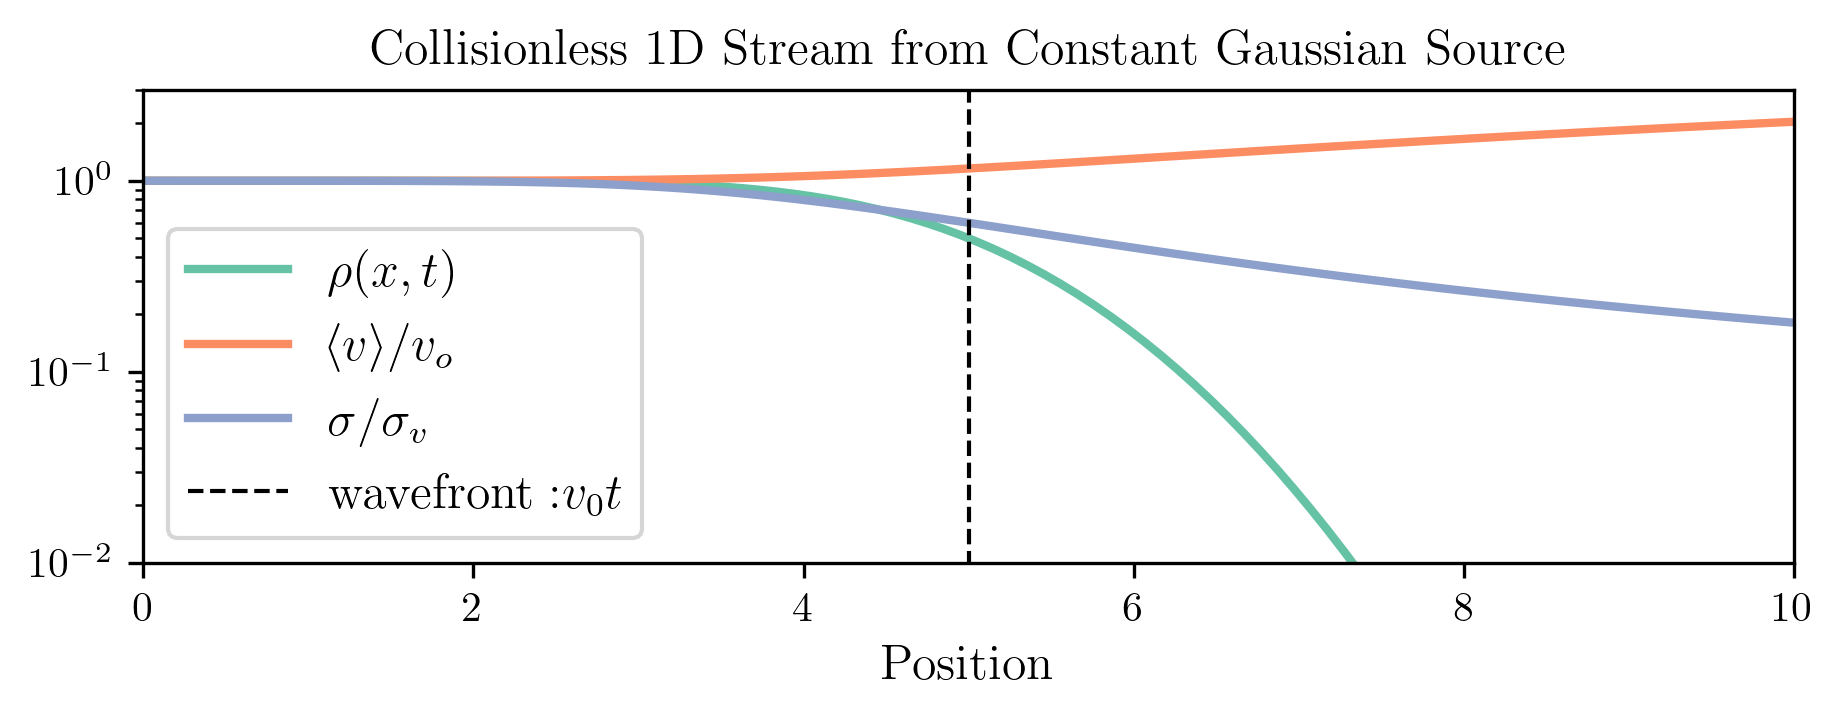
\includegraphics[width=\linewidth]{images/collisionless_1D_stream.png}
                \caption{A snapshot at a fixed time of selected moments of the distribution function describing one-dimensional collisionless streaming, used here as an approximation for a stellar stream, as given by Eq.~\ref{eq:one_dimensional_collisionless_streaming}. Particles are continuously injected at the origin with velocities drawn from a Gaussian distribution with mean $v_0 $ and dispersion $ \sigma_v$. Shown are the particle density, local mean velocity, and local velocity dispersion, all normalized. }
                \label{fig:collisionless_1D_stream}
            \end{figure}


            \textit{Note:} I would love to explore this more rigorously in the context of time-dependent or eccentric mass loss, where the source term becomes periodic. I did begin studying such a model using a time-dependent Gaussian source, but at some point the ``simple approach'' becomes as complex as full numerical simulations. 

            





\section{The Ignored Physics} \label{sec:ignoredphysics}
    Of course, this section could be extremely large since not all of physics are relevant for this problem. Schrodinger's equation, or maxwells equation are irrelvant. But that's not the point of this section. In the previous two sections I wanted to present our methods and justify that they are appropriate to gain insight to stellar streams emerging from galactic globular clusters. In this section, I want to lay out the landscape of what we're missing and other techinques presented in the literature. The most important of which is certainly handing the globular cluster as a collisional system. 

    Make some notes on the time evolution of the Milky Way's gravitational field. Say that, instead of considering this to be \textit{ignored}, it's on the too-do list. The most important thing that I want to comment on is the internal dynamics of the globular clusters since I previece this to be the main limited factor in terms of interpretability of our results. \dots. 
     

    \subsection{Globular Cluster Internal Dynamics} \label{sec:collisionalDynamics}
        In this thesis, globular clusters are the \textit{source} for stellar streams, because we are interested in stellar streams more than we are interseted in the globular clusters. We simplified the orbits of stars within clusters to feel the mean-field, knowing full well that this is a limiting assumption. We traded computational speed for accuracy. However, how much of a limiting assumption is this? In essence, by simplifying the dynamics of the globular cluster with a test-particle method, we are limiting our models fidelity of how many star-particles escape at any unit time, how they are ejected, and which stars go where. Below, I would like to present a basic demosntration of two-body relaxation and then summarize other papers that explore these works a little bit. 


        \subsubsection{Two-body Relaxation Time: a derivation and example}
            While it is appropriate to treat the orbits of stars in galaxy as collisionless, this approximation breaks down in the context of globular clusters. Here, I present a brief numerical experiment to illustrate the concept of two-body relaxation, which quantifies the breakdown of the mean-field approximation.

            Two-body relaxation asks: how long does it take for the discrete, granular nature of the stellar medium to cause a star's trajectory to deviate significantly from the one it would follow in a perfectly smooth (mean-field) potential? This timescale is defined by the condition: $\delta v / v_0 \sim 1$, meaning that the change in the velocity due to the medium roughly the original speed.

            In this context, we simplify the star's motion, neglecting the complexity of orbital paths in a galaxy. Instead, we consider uniform motion through a medium composed of discrete masses. If the medium consists of many small-mass particles, the potential is smoother and better approximates the mean field. If there are fewer particles with larger mass, each interaction can cause a significant deflection.

            For a single interaction in the impulse approximation, the change in velocity is:
            \begin{equation}
                \delta \mathbf{v} = \frac{Gm}{bv} \begin{bmatrix} 0 \\ \cos\theta \\ \sin\theta \end{bmatrix},
                \label{eq:delta_v_vec_impulse_approx}
            \end{equation}
            where $b$ is the impact parameter, $m$ the perturber's mass, $v$ the relative velocity, and $\theta$ the angle in the transverse plane. These impulses deflect the star sideways but not along the direction of motion — a key assumption in the impulse approximation.

            Now consider not just one fly-by, but a sequence of them. A real galaxy has a radially decreasing density, so a star never sees a symmetric distribution unless it's exactly at the center — but we are interested in fluctuations from the mean field, not the mean field itself. That is, if $\Phi_\mathrm{MW} = \Phi_\mathrm{mean}(\vec{r}) + \Phi_\mathrm{stochastic}(\vec{r})$, we are isolating the stochastic part.

            To simplify further, we idealize the galaxy as a cylinder of radius and length $R$, with uniform number density $n = N_p / (\pi R^3)$. As the star moves through this medium, we apply Eq.~\ref{eq:delta_v_vec_impulse_approx} to compute cumulative velocity kicks. This is demonstrated numerically in Fig.~\ref{fig:twoBodyRelaxation}.

            \begin{figure}
                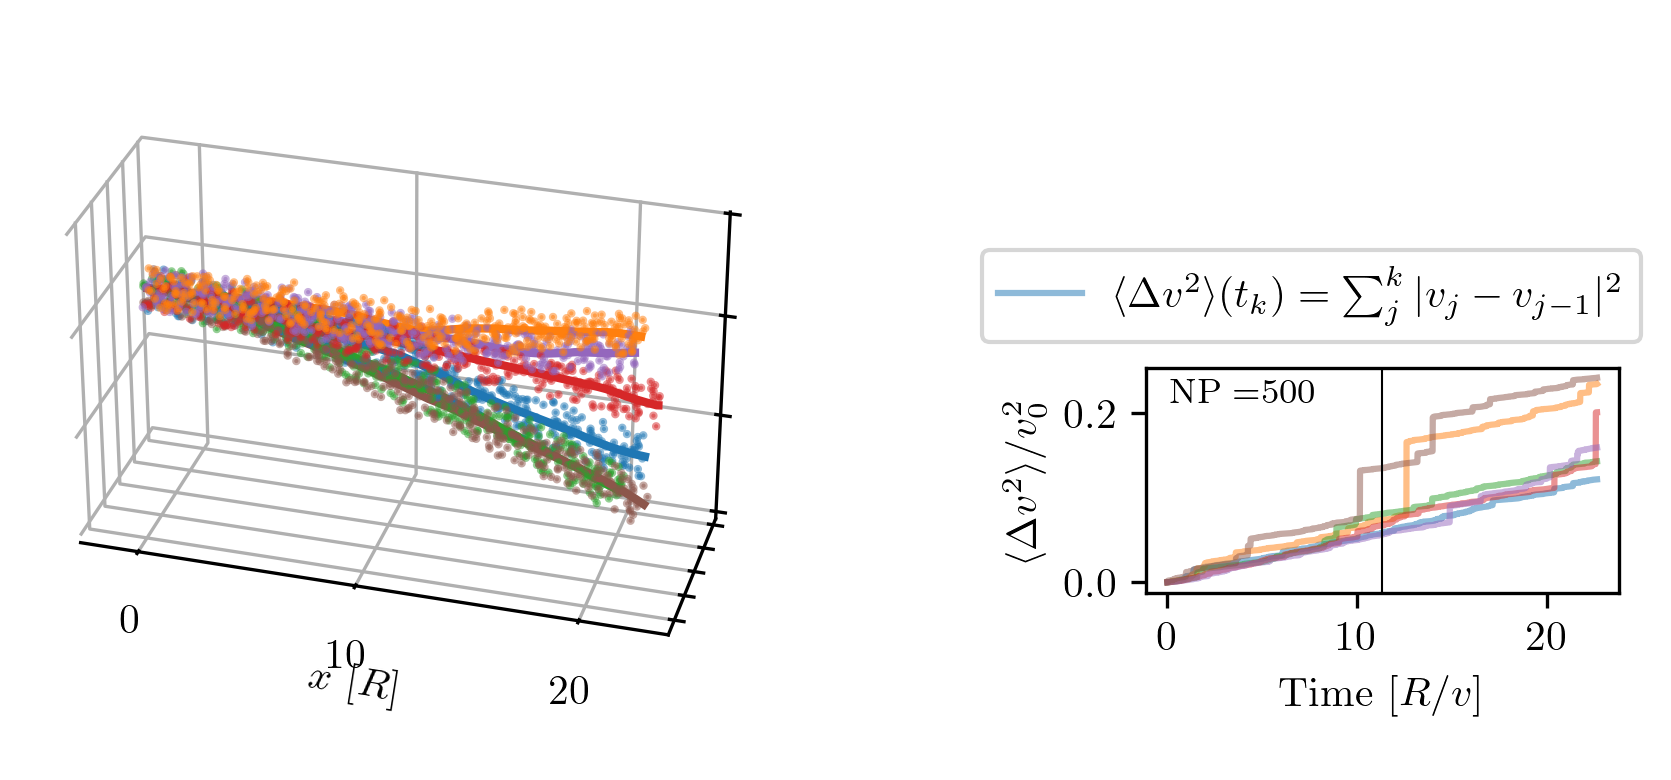
\includegraphics[]{images/twoBodyRelaxation.png}
                \caption{Demonstration of two-body relaxation. A star travels through a medium with uniform number density ($n = 500/\pi R^3$). Six independent trajectories are shown, each sampling a different realization of the same underlying number density. Particles are generated on-the-fly as the star moves. The right panel shows the cumulative squared change in velocity. The vertical line indicates the theoretical two-body relaxation time}
                \label{fig:twoBodyRelaxation}
            \end{figure}

            To perform this experiment, I normalize units such that $G = M = R = t_\mathrm{cross} = 1$, giving $v_0 = 1$ and $m = M/N_p$. For Fig.~\ref{fig:twoBodyRelaxation}\footnote{The two-body relaxation experiment is purely illustrative. Despite multiple attempts, I was unable to make the numerical results consistent with the theoretical prediction. Not only is the relaxation process significantly slower than expected, but the discrepancy also worsens with increasing particle number. I rewrote the script several times but was unable to identify the issue. Nonetheless, the main takeaway remains valid: gravitational two-body encounters induce a random walk in velocity space.}, $N_p = 500$, so the number density is $500/\pi$. 

            At each timestep $dt$, a cylindrical volume $\pi R^2 v dt$ is populated with a Poisson-sampled number of particles, where the expected number is $\langle N_{p,\mathrm{disc}} \rangle = n \pi R^2 v dt$. Each particle contributes a velocity kick via Eq.~\ref{eq:delta_v_vec_impulse_approx}, which is summed over time to compute the net velocity and trajectory.

            I would like to present some key steps in the theoretical derivation. In this idealized model, we expect:
            \begin{equation}
                \langle \delta \mathbf{v} \rangle = \mathbf{0},
            \end{equation}
            since the medium is isotropic and random, so kicks cancel on average. However, the mean squared change is non-zero:
            \begin{equation}
                \left\langle \delta v^2 \right\rangle \neq 0.
            \end{equation}
            $\left\langle \delta v^2 \right\rangle$ can be found by reasoning on the number of expected interactions from each shell of a cylinder, where the volume infinitesimal is: $rd\theta dr(vdt)$. We find that this \textit{diffusion} grows linearly with time, and its rate of change gives the two-body relaxation timescale:
            \begin{equation}
                \tau_\mathrm{2-body} = \frac{v_0^2}{\frac{d \left\langle \delta v^2 \right\rangle}{dt}}.
            \end{equation}

            Another key in this derivation is the Coulomb integral, which involves a logarithmic divergence:
            \[
            \int \frac{1}{R} \, dR.
            \]
            We must regularize this with appropriate limits. The upper limit is the system size (no perturbers beyond this). The lower limit corresponds to where the impulse approximation breaks down — I choose the distance at which a star becomes gravitationally bound to the perturber, though this is generous and the impulse approximation breaks down at larger distances.

            The resulting expression for the two-body relaxation time is:
            \begin{equation}
                \tau = t_\mathrm{cross} \, \frac{N}{8 \ln(N/2)}.
            \end{equation}

            Let's apply this to globular clusters using their catalog values. Take the median crossing time per star as
            \[
            t_\mathrm{cross} = \sqrt{\frac{r_{1/2}^3}{GM}},
            \]
            assuming an average stellar mass of 0.8 $M_\odot$ [citation needed]. With this, only a handful of clusters have relaxation times greater than the 5 Gyr integration time used in our simulations. These include: 
            
            \textit{NGC~2419, NGC~5139, Pal~14, Pal~15, FSR1758, Ter~8, Sagittarius~II.}

            Across the catalog, the average relaxation time is 1.5 Gyr, the median is 0.8 Gyr, the maximum is 21 Gyr, and the minimum is 0.03 Gyr.




    
        
        \subsubsection{Beyond Two-Body Relaxation}
            By modeling globular clusters with the restricted three-body problem, we neglect mass loss due to internal dynamics. Ignoring this has a consequence. The number density, extension, and luminosity of the stream can be greatly influenced by the internal dynamics. The internal dynamics involve a rich variety of physical processes that not only drive their internal evolution but also contribute to stellar escape through mechanisms other than tides. Many of these processes are reviewed in \citet{2003gmbp.book.....H} and have been the subject of decades of study \citep{1978RvMP...50..437L,1990ApJ...351..121C,1997A&ARv...8....1M}. Interestingly, many macrophysical behaviors emerge from microscopic interactions, such as repeated two-body encounters or three-body interactions. In this section, I focus on how these internal processes can affect the morphology and properties of the stellar streams that globular clusters produce.

            To begin, recent works by \citet{2023MNRAS.518.4249G,2024MNRAS.528.5189G} performed a study similar to our Chapter~4. While we investigated the mass loss of the globular cluster catalog due to tidal stripping, they examined the cumulative mass loss induced by three-body interactions within globular cluster cores. An example of this mass ejection distribution is shown in Fig.~\ref{fig:grondin_et_al_core_spray}. Indeed, globular clusters host many binary systems that can significantly influence cluster dynamics. As \citet{2024MNRAS.528.5189G} describe, a third star engage with the binary leading to the ejection of one star with significant kinetic energy. Such velocities can exceed the cluster escape velocity. Not only the energy be high enough to escape, but it may be so high has completely erase the effective potential barrier (Fig.~\ref{fig:CR3BP_forbidden_region}) and escape in any direction. The result is a population of stars that escape in a more isotropic and diffuse manner than those lost through tidal stripping alone.
            \begin{figure}
                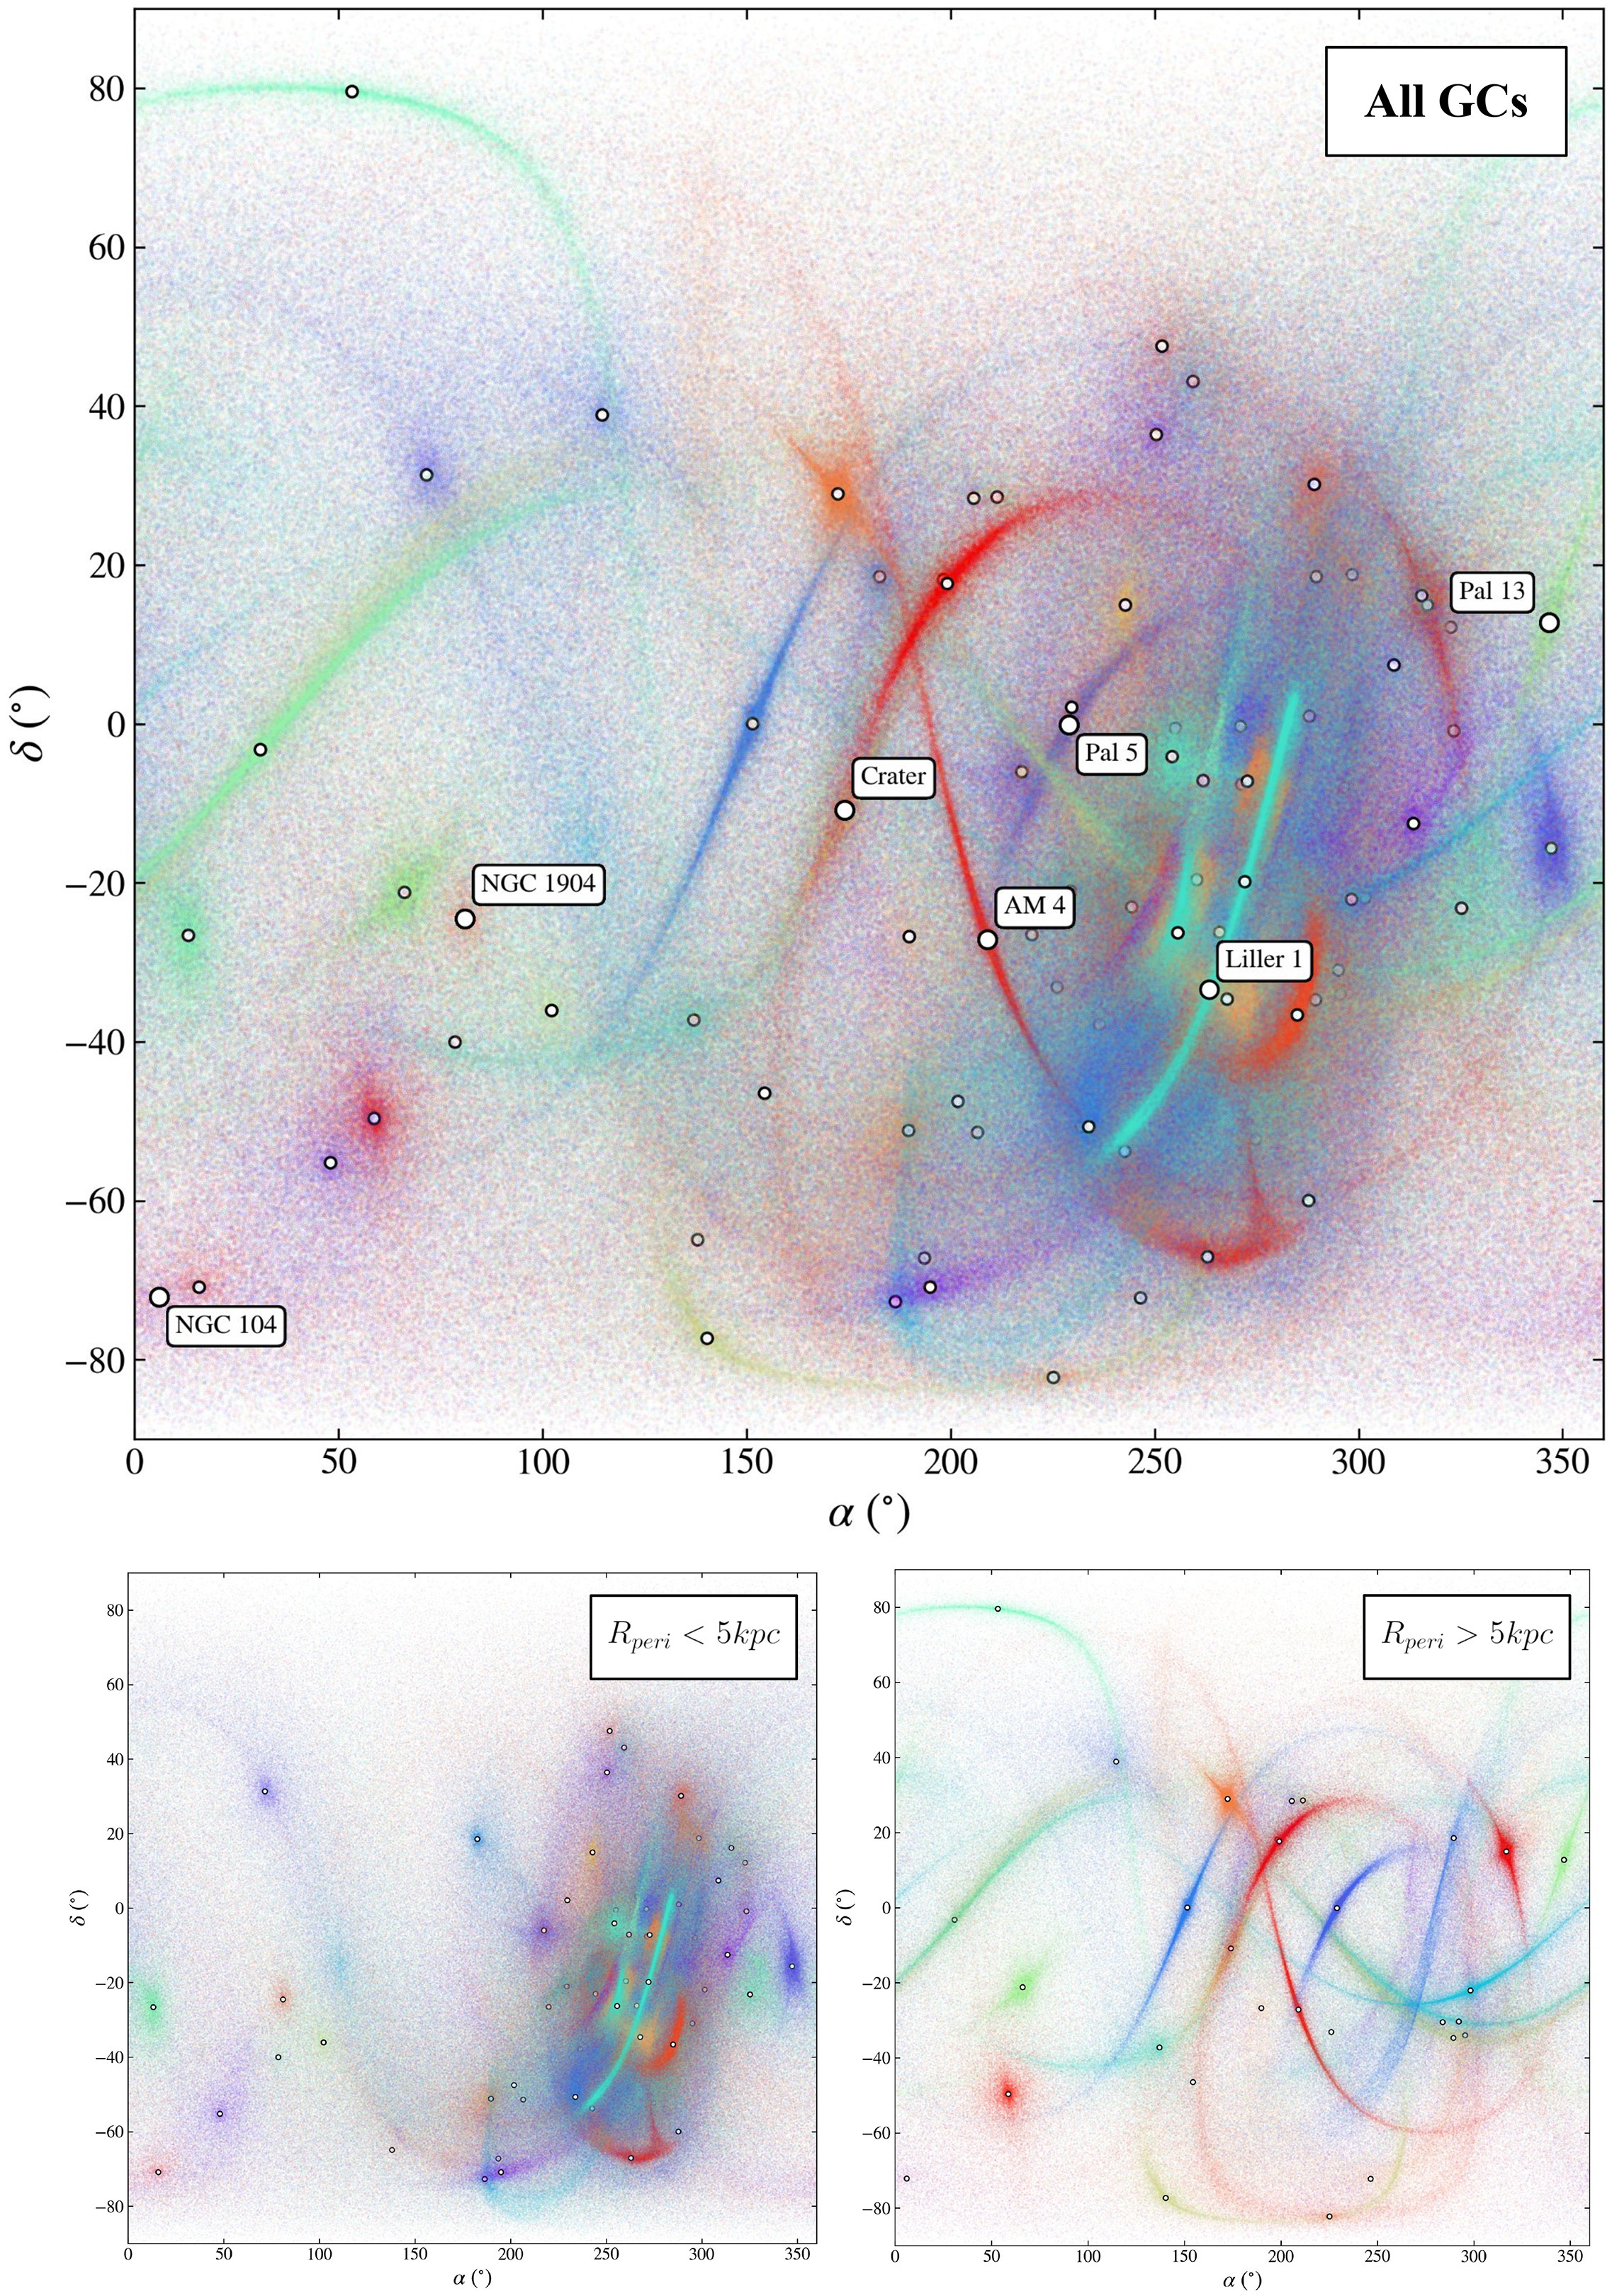
\includegraphics[width=\linewidth]{images/grondin_et_al_core_spray.jpeg}
                \caption{Expected distribution of stars from the Milky Way globular clusters that are ejected from globular cluster cores via 3-body interactions. Reproduced from \citet{2024MNRAS.528.5189G}.}
                \label{fig:grondin_et_al_core_spray}
            \end{figure}            

            These high-velocity escapers are of particular interest in light of stars in the Gaia catalog that appear to exceed the Galactic escape speed \citep{2021ApJS..252....3L}. Proposed origins for these stars include supernova kicks within binary systems, where one component goes supernova and imparts a substantial recoil to the companion, or dynamical ejections from dense cluster cores. Some studies even suggest that globular clusters may contribute to the population of hypervelocity stars.
            
            Not only do we gain a lot of physics when we consider the stars to have mass, but we gain even more when we consider the stars to have a distribution of masses. \citet{1955ApJ...121..161S} proposed one of the first stellar mass functions based on stellar counts. A current popular model is that of \citet{2001MNRAS.322..231K} who created a piece-wise mass function to account for the lower end of the distribution tapering off. By introducing such a mass function to the globular clusters, a suite of physics is unlocked. One well-known example is \textit{dynamical friction} \citep{1943ApJ....97..255C,1943ApJ....97..263C,1943ApJ....98...54C}, which describes how massive bodies lose orbital energy through interactions with less massive ones, causing them to sink toward the center of the cluster. This process is the basis for \textit{mass segregation}, in which massive stars concentrate toward the center. The underlying statistical tendency is toward energy equipartition, where the average kinetic energy per particle is constant across the system. Since $E \propto m \langle v^2 \rangle$, this implies $\langle v^2 \rangle \propto 1/m$. However, in real clusters, relaxation times can be long, and equipartition may remain incomplete over the cluster lifetime \citep{2016MNRAS.458.3644B,2025A&A...698A.209Z}. Moreover, since tides preferentially remove the stars on the most weakly bound (i.e., high-energy) orbits, they tend to strip low-mass stars first.

            Next, not only can we consider the the implications of modeling the stars to have mass, but also what we cain when considering them to be actual stars, i.e., luminous, gaseous bodies in hydrostatic equilibrium. By relaxing this constraint, an even more complex picture emerges. Stars vary in mass, age, and composition, which affect their luminosity and detectability. \citet{2008A&A...490..151K} demonstrated that low-mass stars and stellar remnants like white dwarfs preferentially escape from the clusters, which effects the global luminosity profile of a cluster. \citet{2018MNRAS.474.2479B} took this a step further explored how internal cluster dynamics shape the escape of stars with different luminosities. They arrived at a seemingly paradoxical result: more massive clusters can produce \textit{less detectable} stellar streams. The reason is twofold: more massive clusters harbor more low-mass stars, which are intrinsically dimmer, and these same stars are preferentially stripped due to mass segregation. The resulting streams, though potentially more massive, are fainter and harder to detect (see Fig.~\ref{fig:balbinot-2018}).

            \begin{figure}
                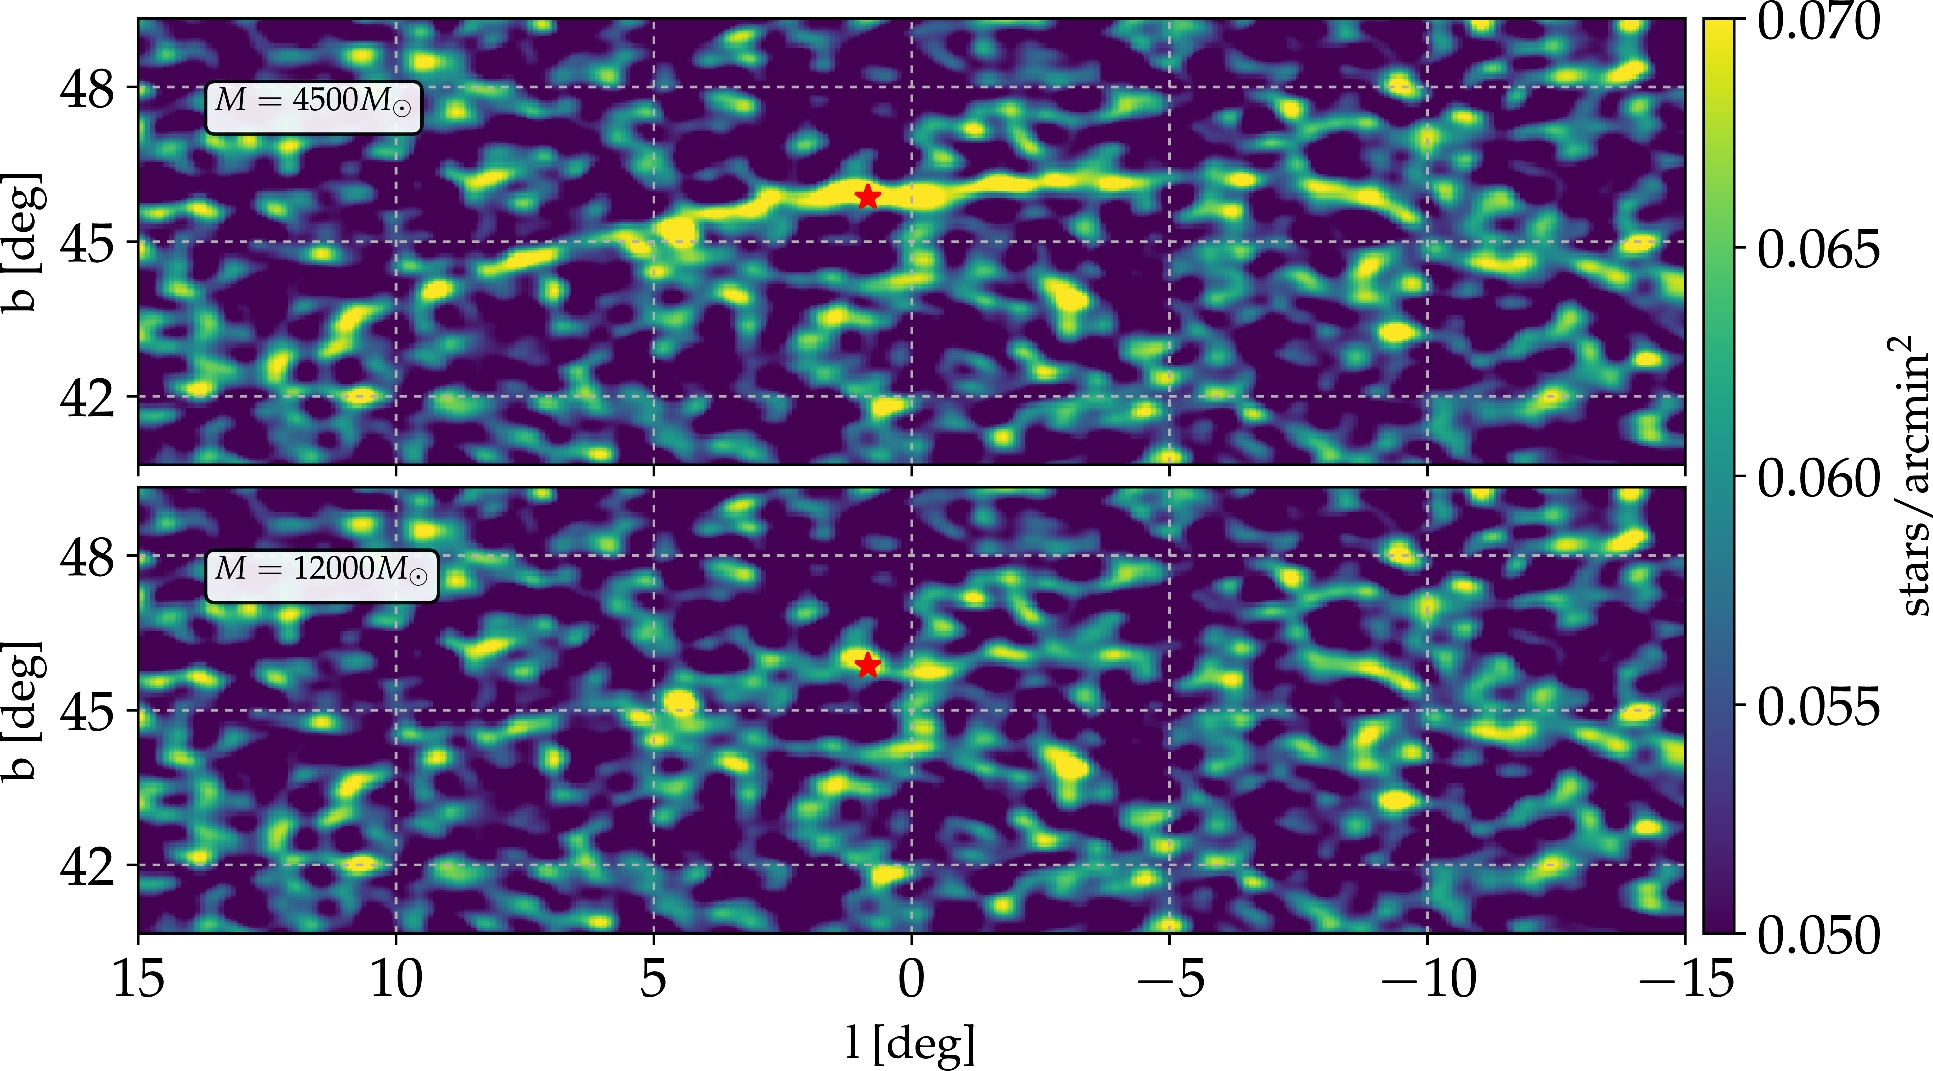
\includegraphics[width=\linewidth]{images/balbinot-2018.jpeg}
                \caption{The effects of stellar evolution on the visibility of stellar streams. Reproduced from \citep{2018MNRAS.474.2479B}.}
                \label{fig:balbinot-2018}
            \end{figure}

            Not only do the stars have luminosities, and that their luminosities change as they evolve, but stellar evolution can also contribute to the dynamics of the system. \citet{2018MNRAS.474.2479B} incorporated stellar evolution in their simulations, capturing its effects on cluster evolution. The most significant contribution occurs during the first $\sim$1~Gyr, when massive stars end their lives as supernovae. These events eject mass from the cluster, shallowing its potential well. \citet{2010MNRAS.409..305L} showed that the mass loss can be broken down in two three phaes, the first mass loss phase is early in  the cluster life and is dominated by stellar evolution. which means the super-novae of the exploding stars can just ejected the stellar material outside of the cluster. if it was in a binary system then it can also eject a low-mass star. The authors note that this does strongly depend on the initial metallicity of the cluster and the initial mass function.
            \footnote{I once wondered whether the kinetic energy injected into surrounding stars by a supernova's ejecta might be dynamically important. A back-of-the-envelope calculation shows it is negligible and mass of the exploded stars wisps out of the cluster.} The early stages of globular cluster evolution is particularly for our purposes, since our simulations begin 5~Gyr ago, and all clusters considered are much older.

            Indeed, future extention of our models to improve genreality of our results can include some internal evolution of the globular cluster dynamics, potential using prescriptive methods since we want to still have cheap computations so that we can explore a large set of the parameter space. Perhaps we could create a partilce spray method like that of the Fardel that is employed in the works of Bonaca or Bovy. However, we would have to ensure that the mass loss is linked to the tidal field. We also want to make sure that the some of the internal considerations can be well modeled like the binary fraction, metalicity, age, and initial mass function. With this, we can begin to engage with detectability of the streams to make better comparisons with our simulated catalog with the observations \dots

    

\chapter{Numerical methods}
As is oftentimes the case when aiming to model realistic physical systems, the equations of motion presented here do not admit closed-form analytical solutions. As such, we must rely on numerical methods and computer simulations to solve them. Specifically, we solve $N$ independent sets of Hamilton's equations, each consisting of six first-order, coupled differential equations.

Numerical integration presents several challenges. First, there is the practical question: how do we actually solve these equations? How can we be confident that our numerical solutions faithfully approximate the true dynamics, especially when the true solution is unknown? How do we handle performance, data volume, or the trade-offs between speed and accuracy?

To do this, I chose to write my own code, \texttt{tstrippy}, despite other codes on the market already existing \citep{2013A&A...557A..84P,2015ApJS..216...29B,2015MNRAS.450.4070W,2017JOSS....2..388P,2018arXiv180208255V}. My motivation was part practical: I wanted to avoid installation difficulties, steep learning curves, and uncertainty over whether existing tools could implement my specific setup. But above all else, I wanted to try my hand at it.  

This chapter documents how we solve the equations of motion numerically, how we validate the accuracy of the solutions, and how the code is organized under the hood.

\section{Astronomical units and scaling}
    When writing any code, the choice of units is important. Astronomical units are rarely the same as SI units. Their creation were often times observationally and historically motivated, resulting in a system that uses multiple units for the same physical quantity, which can be confusing at first.

    For instance, sky positions are typically reported in spherical coordinates. Right ascension (analogous to longitude) is often expressed in either degrees or hours, while declination (similar to latitude) is given in degrees. Distances are reported in parsecs when derived from parallax measurements. Line-of-sight velocities, obtained via spectroscopic Doppler shifts, are reported in kilometers per second. Proper motions describe angular displacements over time on the sky and are usually reported in milliarcseconds per year. Already, we encounter several different units for angles (degrees, hours, arcseconds), time (years, seconds), and distance (km, kpc), none of which align with SI's standard units of radians, seconds, or meters, as summarized in Table~\ref{tab:units}.
    \begin{table}[]
        \caption{Units for various astronomical quantities in Galactic and SI systems.}
        \label{tab:units}
        \begin{tabular}{l|l|l|l|l|l|l|}
                            & Distance  & RA                     & DEC                    & \textbf{$\mathrm{v}_\mathrm{LOS}$} & $\mu_\alpha$ & $\mu_\delta$ \\ \hline
            Galactic: & {[}kpc{]} & {[}deg{]} {[}HHMMSS{]} & {[}deg{]}              & km/s                      & {[}mas/yr{]} & {[}mas/yr{]} \\ \hline
            S.I.       & {[}m{]}   & {[}rad{]}              & {[}rad{]}              & m/s                       & {[}rad/s{]}  & {[}rad/s{]}  \\ 
        \end{tabular}
    \end{table}
    This raises practical concerns—for example, what would be the unit of acceleration? km/s$^2$? parsec/year/second? To systematically manage units, we turn to dimensional analysis, notably the Buckingham Pi theorem \parencite{1914PhRv....4..345B}. In classical mechanics, physical quantities are typically expressed in terms of three fundamental dimensions: length, time, and mass. Any quantity can then be represented as a product of powers of these base units:
    \begin{equation}
        \left[\mathrm{Quantity}\right] = l^a t^b m^c =
            \begin{bmatrix}
                a\\
                b\\
                c 
            \end{bmatrix}
    \end{equation}
    For example, velocity has dimensions $[1, -1, 0]$, momentum is $[1, -1, 1]$, and acceleration is $[1, -2, 0]$.

    It is not strictly necessary to adopt length-time-mass as the fundamental basis, as long as the three chosen base units are linearly independent. In stellar dynamics, it is often more natural to use distance, velocity, and mass as the base units. In this thesis, we adopt:
    \begin{itemize}
        \item Distance: 1~kpc
        \item Velocity: 1~km/s 
        \item Mass: 1~solar mass $\mathrm{M}_\odot$
    \end{itemize}

    In this system, time has derived units of:
    \begin{equation}
        \left[t\right] = \frac{\mathrm{distance}}{\mathrm{velocity}} = \frac{\mathrm{kpc}}{\mathrm{km/s}}.
    \end{equation}
    While not immediately intuitive, this unit of time is convenient because:
    \begin{equation}
        1\mathrm{Gyr} \approx 1~\mathrm{s}\cdot\frac{\mathrm{kpc}}{\mathrm{km}}.
    \end{equation}

    The gravitational constant has dimensions:
    \begin{equation}    
        \left[G\right]=\frac{v^2 \cdot l}{m},
    \end{equation} 
    which evaluates numerically to: 
    \begin{equation}
        G = 4.301 \times 10^{-6} \left(\mathrm{km}/\mathrm{s}\right)^2 \cdot \mathrm{kpc} \cdot \mathrm{M}_\odot^{-1}.
    \end{equation}
    Once the base units are defined, derived quantities such as acceleration follow directly. Whether considering acceleration as $v^2~l^{-1}$ or $l \cdot t^{-2}$, they are equivalent and yield: $\left(\mathrm{kpc}/\mathrm{s}\right)^2 \cdot \mathrm{kpc}^{-1}$.

    It is worth mentioning that $N$-body codes often select distance, velocity, and the gravitational constant as the base units, setting $G = 1$. While this choice simplifies force computations, it introduces less intuitive units for mass. For instance, by choosing 1~kpc for distance and 1~km/s for velocity, and setting $G = 1$, the derived mass unit becomes:
    \begin{equation}
        \left[\mathrm{mass}\right] = \frac{l \cdot v^2}{G} = 232509~\mathrm{M}_\odot.
    \end{equation} This approach was used in our first paper (see Chapter~4). 
    The famous galactic dynamical python code, \texttt{Galpy} makes a different choice and introduced \textit{natural units} \citep{2015ApJS..216...29B}. More specifically, \citet{2015ApJS..216...29B} uses a normalization in which $R$, the cylindrical scale length of the galaxy, and $v_\mathrm{circ}$, the circular velocity at this radius, are both set to 1. This choice is motivated by a galaxy's rotation curve and is embodied in:
    \begin{equation}
        \frac{v_\mathrm{circ}^2}{R_0} = \nabla  \Phi \left(R_0, z=0\right).
        \label{eq:vcirc}
    \end{equation}
    Note that the gravitational constant is also set to 1. Whatever the form of the potential, the scale lengths must be normalized to $R$, and the mass parameter is subsequently determined through Eq.~\ref{eq:vcirc}. The total potential is a linear combination of individual components, with the user selecting the contribution of each component to the force at the characteristic radius. For example, $\Phi = \sum_i a_i\Phi_i$, where $a_i$ are weights such that $\nabla \Phi_i(R_0, z=0) = a_i$ in normalized units. In this system of units, emphasis is placed on the rotation curve and how much each component contributes to it at the reference radius of the galaxy. Note that $v_\mathrm{circ}(R_0)$ is not necessarily the maximum rotational velocity.

    In short, each code presents its own preferred units and normalization. \texttt{Tstrippy}, by contrast, expects the user to pass masses in solar masses, velocities in kilometers per second, and distances in kiloparsecs. However, physical constants are not hard-coded, so the user may pass any numerical values to the code as long as they are based on a self-consistent unit system. Nonetheless, the code comes equipped with parameters for the \texttt{pouliasis2017pii} potential \citep{2017A&A...598A..66P} and for the catalog of globular clusters \citep{2018MNRAS.478.1520B} in units of kpc, km/s, and $\mathrm{M}_\odot$.

    A valid general strategy when developing numerical codes is to implement a module that converts user-defined units to the internal units. This functionality also exists in \texttt{Galpy} and a similar system is implemented in \texttt{Agama} \citep{2018arXiv180208255V}. I chose not to add such a layer to \texttt{Tstrippy} since \texttt{Astropy} provides an excellent unit-handling module that allows users to convert between units easily \citep{2013A&A...558A..33A}, and I recommend its use in the documentation. 

\section{Solving the equations of motion}
    Long before the advent of computers, Euler (1707-1783) proposed a simple method for numerically solving differential equations. In this method, a solution is approximated by
    \begin{equation}
        y_{i+1} = y_i + \Delta t \frac{dy}{dt}\left(y_i,t_i\right),
    \end{equation}
    where \( i \) is a timestep index. This means that at each point \( (t_i, y_i) \), the function is extrapolated forward using a linear approximation.

    The accuracy of this method can be understood using a Taylor series expansion of the exact solution \( y(t_i + \Delta t) \) about \( t_i \):
    \begin{equation}
        y(t_i + \Delta t) = y(t_i) + \Delta t y'(t_i) + \frac{1}{2!}\Delta t^2 y''(t_i) + \dots
    \end{equation}
    Euler's method captures only the first two terms. The difference between the exact solution and the Euler estimate is dominated by the second-order term. Thus, the \textit{local truncation error} (error per step) is
    \[
    \mathrm{Err}_{\mathrm{step}} \approx \frac{1}{2} \Delta t^2 y''(t_i) = \mathcal{O}(\Delta t^2).
    \]

    The \textit{global error} (accumulated over many steps) is approximately the number of steps times the average error per step:
    \[
    \mathrm{Err} \approx N_{\mathrm{step}} \cdot \langle \mathrm{Err}_{\mathrm{step}} \rangle \approx \frac{T}{\Delta t} \cdot \Delta t^2 \langle y'' \rangle = \mathcal{O}(\Delta t).
    \]
    This means that halving the timestep roughly halves the global error.

    It is important to note that using a taylor series to estimate the error is not mathematically rigorous and not always generalizable. The actual error behavior depends strongly on the properties of the function being integrated. For instance:
    \begin{itemize}
        \item If \( y \) is linear in \( t \), then \( y' \) is constant and Euler's method gives the exact result.
        \item If \( y(t) = t^a \), the local errors accumulate and grow monotonically.
        \item If \( y \) has curvature that changes sign, local errors can partially cancel out over the course of the integration.
    \end{itemize}
    For a more systematic treatment of integration methods and their error properties, Chapter 16 of \textit{Numerical Recipes in C} provides an excellent introduction \parencite{1992nrca.book.....P}.

    Regardless of the method used, sanity checks are essential to validate the result. These include:
    \begin{itemize}
        \item Trying different integration schemes.
        \item Performing convergence tests to ensure the solution stabilizes as \( \Delta t \to 0 \).
        \item Leveraging any known properties of the solution to verify correctness.
    \end{itemize}
    For example, we can exploit the properties of Hamiltonain systems to design integrators. In this thesis, we implemented the Leapfrog integrator and the Forest-Ruth scheme \citep{bovy_inprep, 1990PhyD...43..105F}. These schemes are derived from the structure of Hamiltonian mechanics and are known as \textit{symplectic integrators}. Before continuing, I would like to quote \citep{bovy_inprep}:
    \begin{quote}
        Hamiltonian integrators are often called symplectic. This name comes from the fact that these integrators are Hamiltonian maps, whose mathematical structure is that of a vector flow on a symplectic manifold. Many fine dynamicists have made great contributions to the field without delving deeply into the meaning of the previous sentence and we do not discuss this further.
    \end{quote}
    However, my curiosity about linguistics pushed me to delve further: What does \textit{symplectic} mean? \citet{weyl1946classical} coined the term because \textit{complex} was already taken. The prefix latin \textit{com}- refers to \textit{together}, and \textit{plexus} comes from greek meaning ``woven'' or ``braided''. Symplectic translates exactly the same way: \textit{sym}- is a Greek prefix for ``together.'' The idea remains the same: in Hamiltonian dynamics, the evolution of position and momentum are interdependent. This becomes clearer in matrix form:
    \begin{equation}
        \begin{bmatrix}
            \dot{\bf{q}}\\
            \dot{\bf{p}}
        \end{bmatrix}
         = 
        \begin{bmatrix}
            0 & I_n \\
            -I_n & 0 
        \end{bmatrix}
                \begin{bmatrix}
            \frac{\partial \mathcal{H}}{\partial \bf{q}} \\
            \frac{\partial \mathcal{H}}{\partial \bf{p}}
        \end{bmatrix}
        \label{eq:symplectic}
    \end{equation}
    Here, the skew-symmetric symplectic matrix ``weaves'' the positions and momenta together.

    Although the equations of motion do not admit analytical solutions, they possess several known properties. First, trajectories governed solely by gravity are time-reversible. This property is important for our methodology, where we integrate the equations of motion backward in time and then forward again to the present-day position. Secondly, the total orbital energy is conserved. Moreover, according to Liouville's theorem, Hamiltonian flows preserve the local phase space volume. A corollary of this is that the determinant of the Jacobian matrix of the transformation from $\left(q,p\right)\rightarrow \left(q',p'\right)$ must be one, which means that the transformation only rotates or translates an infinitesimal volume but does not shrink or expand the volume. We can view the transform as: 
    \begin{eqnarray}
        q' &= q + \frac{\partial \mathcal{H}}{\partial p}\Delta t, \\
        p' &= -\frac{\partial \mathcal{H}}{\partial q}\Delta t + p,
    \end{eqnarray}
    The Jacobian matrix is given by $\left(\frac{\partial x_i'}{\partial x_j }\right)$: 
    \begin{equation}
        \begin{bmatrix}
            1 & \Delta t \frac{\partial^2 \mathcal{H}}{\partial p^2} \\  
            -\Delta t \frac{\partial^2 \mathcal{H}}{\partial q^2} & 1 \\  
        \end{bmatrix}
    \end{equation}
    and the subsequent determinant is: 
    \begin{equation}
        \mathrm{det}\left(J\right) = 1 - \Delta t^2 \frac{\partial^2 \mathcal{H}}{\partial q^2} \frac{\partial^2 \mathcal{H}}{\partial p^2}.
    \end{equation}
    In general, neither $\frac{\partial^2 \mathcal{H}}{\partial q^2}$ or $\frac{\partial^2 \mathcal{H}}{\partial p^2}$ are zero. There is a quick fix to this dilema, namely, only stepping in $q$ or $p$ while holding the other constant. In turn, the transformation of a single step will have a Jacobian whose determinant is 1. The transformation order becomes: $(q,p) \rightarrow (q',p) \rightarrow (q',p')$. This is commonly referred to as a sequence of \textit{drifts} and \textit{kicks}. A \textit{drift} updates the position while holding the momentum fixed, and a \textit{kick} updates the momentum while holding the position fixed. Symplectic integrators alternate these operations in a specific sequence to preserve the Hamiltonian and phase space volume.

    The scheme outlined above is essentially a first-order method and is closely related to Euler's method. More sophisticated integrators use values from multiple timesteps to construct higher-order estimates of the system's evolution. For example, some schemes temporarily evolve the position to an intermediate value $q_\mathrm{temp}$, use this to compute a momentum $p_\mathrm{temp}$, and then adjust both using weighted averages or predictor-corrector steps to reach the final state. These methods carefully balance forward and backward steps to optimize accuracy while preserving the symplectic structure.

    One of the most commonly used symplectic integrators in galactic dynamics is the Leapfrog scheme. It works by interleaving updates of positions and momenta using time-centered averages. Specifically, the average momentum between $q_i$ and $q_{i+1}$ (denoted $p_{i+1/2}$) is used to advance the position, and then the average force (derived from the potential) is used to update the momentum. In Cartesian coordinates—used throughout this thesis—the Leapfrog algorithm can be written as:
    \begin{eqnarray}
        x_{i+1/2} &= x_i + \frac{1}{2} \dot{x}_i \Delta t , \\
        \ddot{x}_{i+1/2} &= -\nabla \Phi(x_{i+1/2}), \\
        \dot{x}_{i+1} &= \dot{x}_i + \ddot{x}_{i+1/2} \Delta t, \\
        x_{i+1} &= x_{i+1/2} + \frac{1}{2} \dot{x}_{i+1} \Delta t. 
    \end{eqnarray}
    As will be shown in the next section, the Leapfrog algorithm is sufficient. However, the question of computational efficiency and numerical accuracy is ever present. Leapfrog uses the two local points about the position and momenta to evolve them. Other schemes can use more points to have more accurate estimations for the local derivatives. 
    
    \citet{1990PhyD...43..105F} proposed one such method for symplectic integrations. The method involves finding roots of high order polynomials which determine the distances about the local point for finding the best estimate of the derivative for evoling the system. The method involves solving a cubic polynomial to determine the optimal coefficients. While the derivation is mathematically involved, the final scheme is straightforward to implement. I implemented this method and tested its efficiency against the Leapfrog and present the results in the following section. There are eight coefficients in this method, which are presented in Table~\ref{tab:forest_ruth_coeffs}.
    \begin{table}[h]
        \centering
        \caption{Velocity (\(c_n\)) and acceleration (\(d_n\)) coefficients for the Forest-Ruth symplectic integrator.}
        \label{tab:forest_ruth_coeffs}
        \begin{tabular}{ccccc|cccc}
            \multicolumn{4}{c|}{Velocity coefficients (\(c_n\))} & \multicolumn{4}{c}{Acceleration coefficients (\(d_n\))} \\
            $c_1$ & $c_2$ & $c_3$ & $c_4$ & $d_1$ & $d_2$ & $d_3$ & $d_4$ \\
            \hline
            $w + \frac{1}{2}$ & $-w$ & $-w$ & $w + \frac{1}{2}$ & $2w + 1$ & $-4w - 1$ & $2w + 1$ & $0$ \\
        \end{tabular}
    \end{table} 
    The coefficients are all based on the solution to the cubic polynomial: $48 w^3 + 24 w^2 - 1 = 0 $. For a single step, the positions and velocities are updated as follows:
    \begin{align} 
        x' &= x + c_n v \Delta t \\ 
        t' &= t + c_n \Delta t \\ 
        \ddot{x} &= \nabla \Phi (x') \\ 
        \dot{x}' &= \dot{x} + d_n \ddot{x} \Delta t,
    \end{align}
    where $n$ is the \textit{mini-step}. Notice that the sum of $\sum_n^4 c_n$ and $\sum_n^4 d_n$ both equal 1, which is a full timestep $\Delta t$. 

    Lastly, it is important to note that the Leapfrog algorithm is symplectic and time-reversible only for Hamiltonians that are both time-independent and separable—that is, where the Hamiltonian can be written as a sum of a kinetic term depending only on momenta, $T(p)$ and whose potential depends only on position $\Phi(q)$. These conditions are satisfied for systems in an inertial frame with conservative forces. This is true when integrating the motion for the center of mass of the globular clusters. However, the Hamiltonian for the integration of the particles does depend on time. So the Leapfrog algorithm may introduce systematic integration errors due to the violation of its underlying assumptions, beyond ordinary rounding errors.

    Similarly, when we integrate the orbits of either the particles or the globular clusters in the Galaxy containing a bar, we are faced with a choice: we can either work in a time-dependent inertial frame, where the potential rotates and the Hamiltonian explicitly depends on time, or we can transform to a rotating frame, in which case the kinetic energy becomes position-dependent due to Coriolis and centrifugal forces, which breaks the necessary criterion of separability: $\mathcal{H}(q,p) = T(p)+\Phi(q)$. In both cases, the standard assumptions of the Leapfrog algorithm are violated.

    Nonetheless, we will continue to use Leapfrog as it remains a robust and efficient integrator for a wide range of astrophysical systems. Its good long-term energy conservation makes it a reasonable approximation even when the ideal assumptions are not strictly met. However, this highlights the need for careful validation: we must verify that the integration errors remain within acceptable bounds, especially in systems with non-separable or time-dependent dynamics. This validation is the subject of the next section.

\section{Numerical Error and Computation Time}
    To ensure the quality of the integration, we perform two main checks. The first is to ensure that the initial orbital energy of a given particle is conserved to high precision. At each timestep, the relative error in the energy conservation is:
    \begin{equation} 
        \mathrm{err}(E(t)) = \left|\frac{E(t) - E_0}{E_0}\right|,
    \end{equation} 
    where $E_0$ is the initial energy and $E$ is the orbital energy at a given timestep $t$. For the case of a globular cluster, the total orbital energy is its own kinetic energy plus its gravitational potential energy in the Galaxy: $E = T(\mathbf{v}_{\mathrm{GC}}) + \Phi_{\mathrm{MW}}\left(\mathbf{x}_{\mathrm{GC}}\right)$, where $\mathbf{x}_{\mathrm{GC}}$ and $\mathbf{v}_{\mathrm{GC}}$ are the cartesian galactocentric position and velocity of the globular cluster. For the case of the $i$-th star-particle within a globular cluster, the potential energy of the cluster is included: $E_i = T(\textbf{v}_i) + \Phi_{\mathrm{MW}}\left(\textbf{x}_i\right) + \Phi_\mathrm{GC}\left(\textbf{x}_i - \textbf{x}_{\mathrm{GC}}\right)$, where $\mathbf{x}_i$ is the position relative to the Galactic center. The same approach holds when a galactic bar is included, the only difference being that the Galactic potential has a time-dependent element. 

    For potentials with the galactic bar, the total energy is not conserved but rather the Jacobi energy, and this is true only for the globular clusters. For the star-particles, the energy is not conserved in the simulations. However, we track the energy particularly when we perform the second check, which is time-reversability.

    To check the time-reversability, we integrate a cluster back in time, and then change the sign of its velocity to subsequently integrate forward in time. If the integration is correct, the cluster should remain on the same trajectory retracing its steps. We investigate this for the following scenarios and show the results below: 
    \begin{itemize}
        \item The globular cluster population orbiting with a static Milky Way potential;
        \item Star-particles orbiting with a stationary and isolated globular cluster;
        \item Full stream generation, i.e., star particles orbiting within a globular cluster that orbits the Galaxy.
    \end{itemize}

    At this stage, I did not have time to perform a full quality check of orbits within the barred potential. However, I refer the reader to the \texttt{tstrippy} documentation, where I demonstrate the time-reversibility of cluster orbits in the barred potential: \url{https://tstrippy.readthedocs.io/en/latest/reverse_integrability_bar.html}.
    



    \subsection{Globular Cluster Orbits in a Static Galaxy}
        The initial conditions for the globular cluster system (positions and velocities) were taken from \citet{2018MNRAS.478.1520B}'s online globular cluster catalog whose data derived from Gaia Early Data Release 3 among other sources \citep{2021MNRAS.505.5957B,2021A&A...649A...1G,2023A&A...674A...1G}. 

        To test the integrator, we integrated the whole globular cluster system for 5~Gyr, and then integrated it back to the initial conditions. We used four timesteps: $10^4,10^5,10^6,10^7$~years which corresponds to $\left[500,5000,50000,500000\right]$ integration steps, respectively. In general, the timestep should scale with the dynamical time of the orbit. In other words, the timestep should be inversely proportional to the orbital energy. The further the system is from the center, a larger timestep can be used to obtain a given numerical error. 
        
        Of course, the timestep does not just simply scale with a body's orbital energy, it should scale with the maximum acceleration experienced in the system. A highly eccentric orbit requires a smaller timestep to properly integrate the motion near the pericenter, compared to a circular orbit at the same orbital energy. To not clutter the graph, Fig.~\ref{fig:numericalErrorLeapfrogVanilla} only present the whole globular cluster system twice, once integrated with the smallest timestep, $10^4$~years, and once with the largest timestep: $10^7$ years.

        \begin{figure}
            \centering
            \includegraphics[width=\linewidth]{images/numericalErrorLeapfrogVanilla.png}
            \caption{Error in orbital energy for the whole globular cluster system with two different timesteps, dt~=~$10^{7}$ and $10^{4}$ years. Each cluster's is colored by its initial orbital energy. The average of the whole system for a given timestep is indicated with dotted and solid black lines, respectively.}
            \label{fig:numericalErrorLeapfrogVanilla}
        \end{figure}
        In Fig.~\ref{fig:numericalErrorLeapfrogVanilla} we can notice that orbits with higher orbital energies (in red) have low numerical error compared to those with lower energies (in blue),  which penetrate deeper in the potential well. It is clear that, for the whole system, $10^7$~years is a timestep that is far too large, however, interestingly enough, for some of the farthest globular clusters, a timestep of 10 million years resolves their orbits to an error of $\langle \Delta E / E_0 \rangle \sim 10^{-5}$, which is still far less than the uncertainties in the energy due to both modeling and observational uncertainties. Note that in both cases, the errors neither accumulate nor grow with time. This is a testament to the quality of the Leapfrog integration scheme, which is designed to conserve the Hamiltonian accurately.

        Fig.~\ref{fig:numericalErrorReverseIntegration} presents the \textit{time reversibility}, or the integrator's ability to retrace its own steps. For each given timestep, I report the difference between the initial integration and the retrace normalized to the mean of the two position's. I perform the same computation for the velocities. The timestep of $10^7$~yr saturates only after 2~Gyr. The distances do not continue to grow becuase the orbital energy only differs by one part in ten, so at later timesteps, the cluster is still within the same region of phase-space, but the retrace is at a completely different location than the initial integration. The errors in the timestep of $10^6$~yrbecome significant, though by the end of the integration period of 5~Gyr they are still only one part in ten thousand. The timesteps of $10^5$ and $10^4$~yr have excellent retraceability and on average, only differ by one part in $10^{-14}$, and are thus only limited by round off error from the use of double precision floating point numbers.
        \begin{figure}
            \centering
            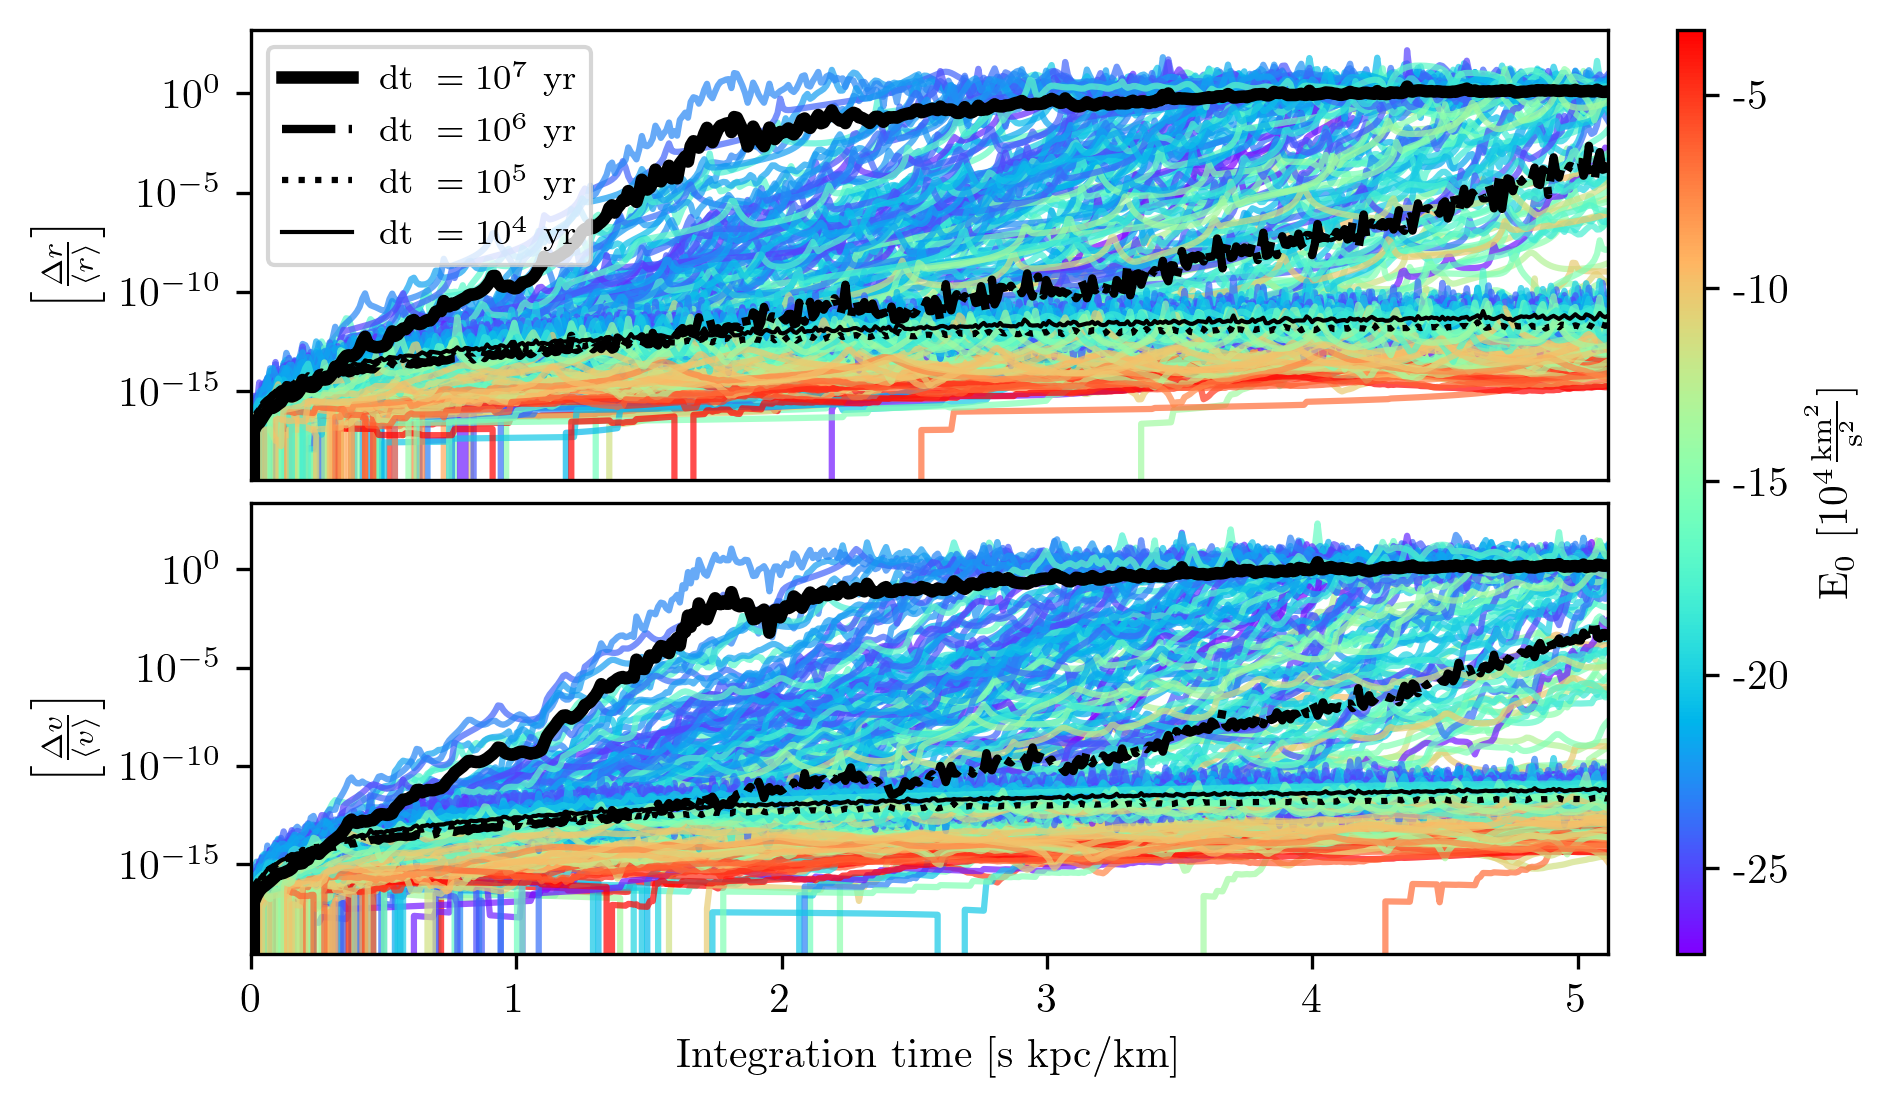
\includegraphics[width=\linewidth]{images/numericalErrorReverseIntegration.png}
            \caption{The \textit{time-reversability} of the Leapfrog scheme for the 165 Galactic globular cluster's for four different timesteps indicated in the legend. The whole system is only shown for $10^4$~yr and $10^7$~yr to avoid clutter. The clusters are color-coded to their initial orbital energy just as Fig.~\ref{fig:numericalErrorLeapfrogVanilla}}
            \label{fig:numericalErrorReverseIntegration}
        \end{figure}

        Computation time is quite important. Fig.~\ref{fig:numericalErrorGlobularClustersComputationTime} presents the total computation time of integrating the globular cluster system, and the time of a single integration step, which is computed by normalizing the total time by the number of objects and number of steps taken: $T_{\mathrm{total}}/N_{\mathrm{GCs}}/N_{\mathrm{steps}}$. In general, the relationship is linear and the integration time per step per object is roughly constant. The downward trend presented in Fig.~\ref{fig:numericalErrorGlobularClustersComputationTime} is in part a coincidence, as some time realizations minimize this, and in part due to the overhead computation time with initializing and finalizing the calculation contributes less and less with increasing integration time. Nonetheless, for this processor (Apple M2 processor), for a single integration step the mean time is $\sim$ 128~nanoseconds. 
        \begin{figure}
            \centering
            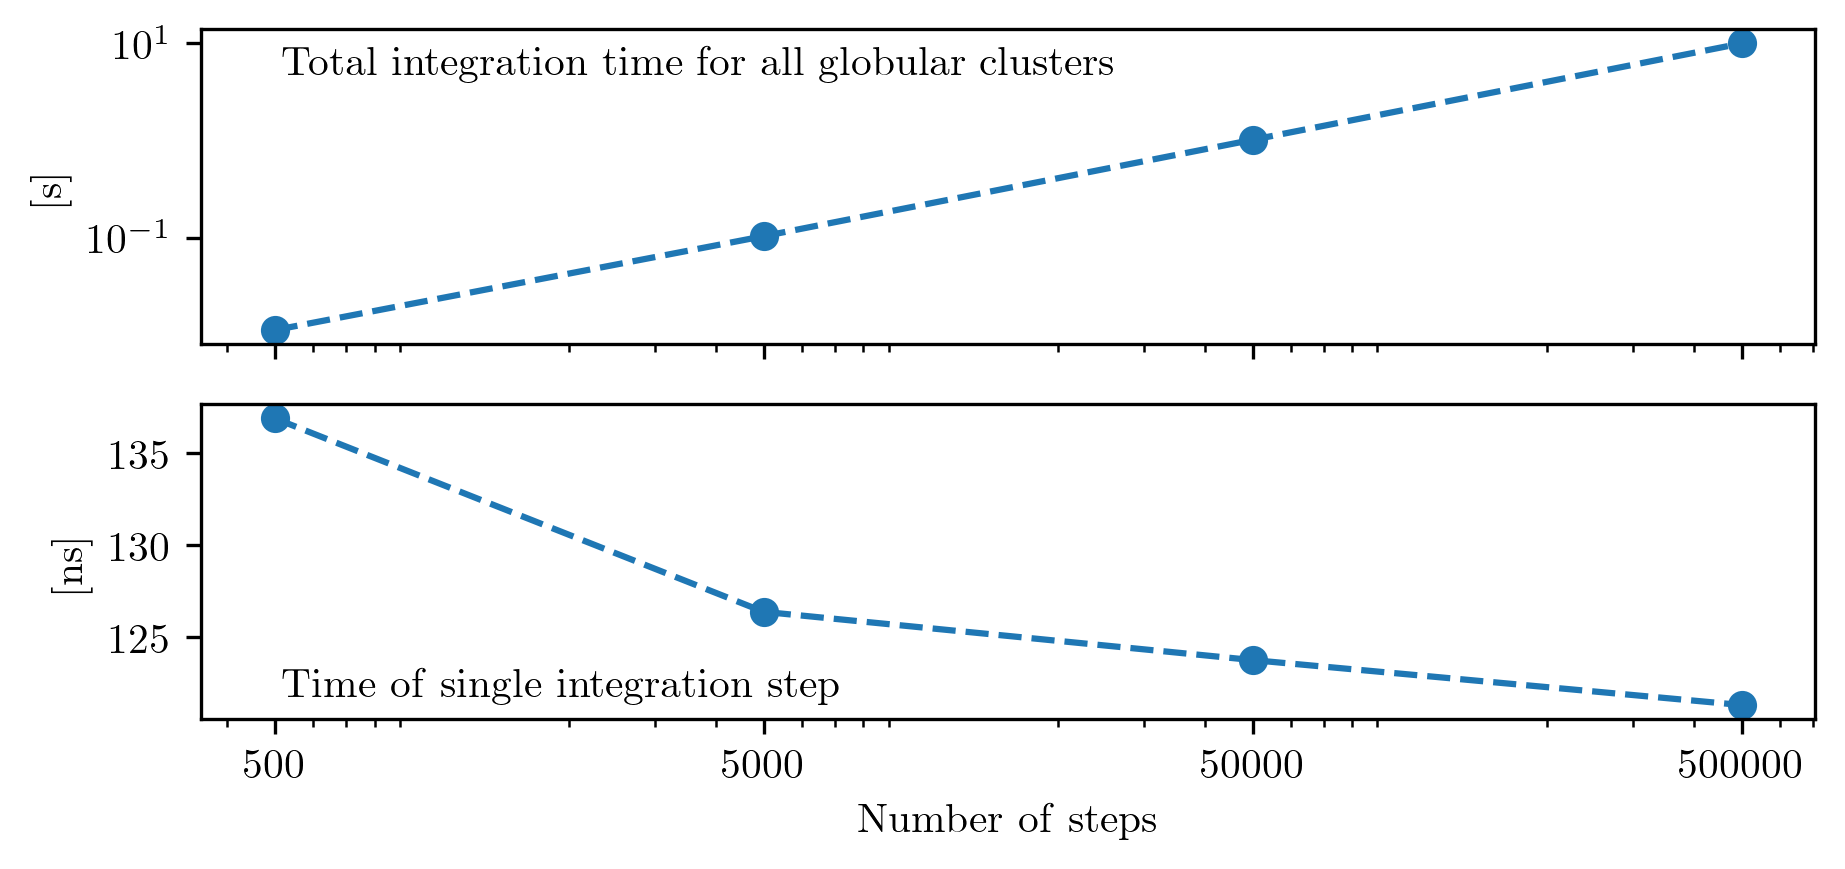
\includegraphics[width=\linewidth]{images/numericalErrorGlobularClustersComputationTime.png}
            \caption{Computation time for integrating the entire globular cluster system using the Leapfrog scheme. The top panel shows the total time while the bottom shows computation time for a single step, for a single object being integrated. This was performed on a 2022 MacBook Air with an Apple M2 processor. }
            \label{fig:numericalErrorGlobularClustersComputationTime}
        \end{figure}

        The Ruth-Forest algorithm discussed in the previous section was implemented and is reported in Fig.~\ref{fig:numericalErrorRuthForest}. Here, as expected, we see that the percision greatly increases when decreasing the timestep. However, since there are four force evaluations for the for a single timestep, this method is naturally slower per step than Leapfrog. How do the two methods compare over all?
        \begin{figure}
            \centering
            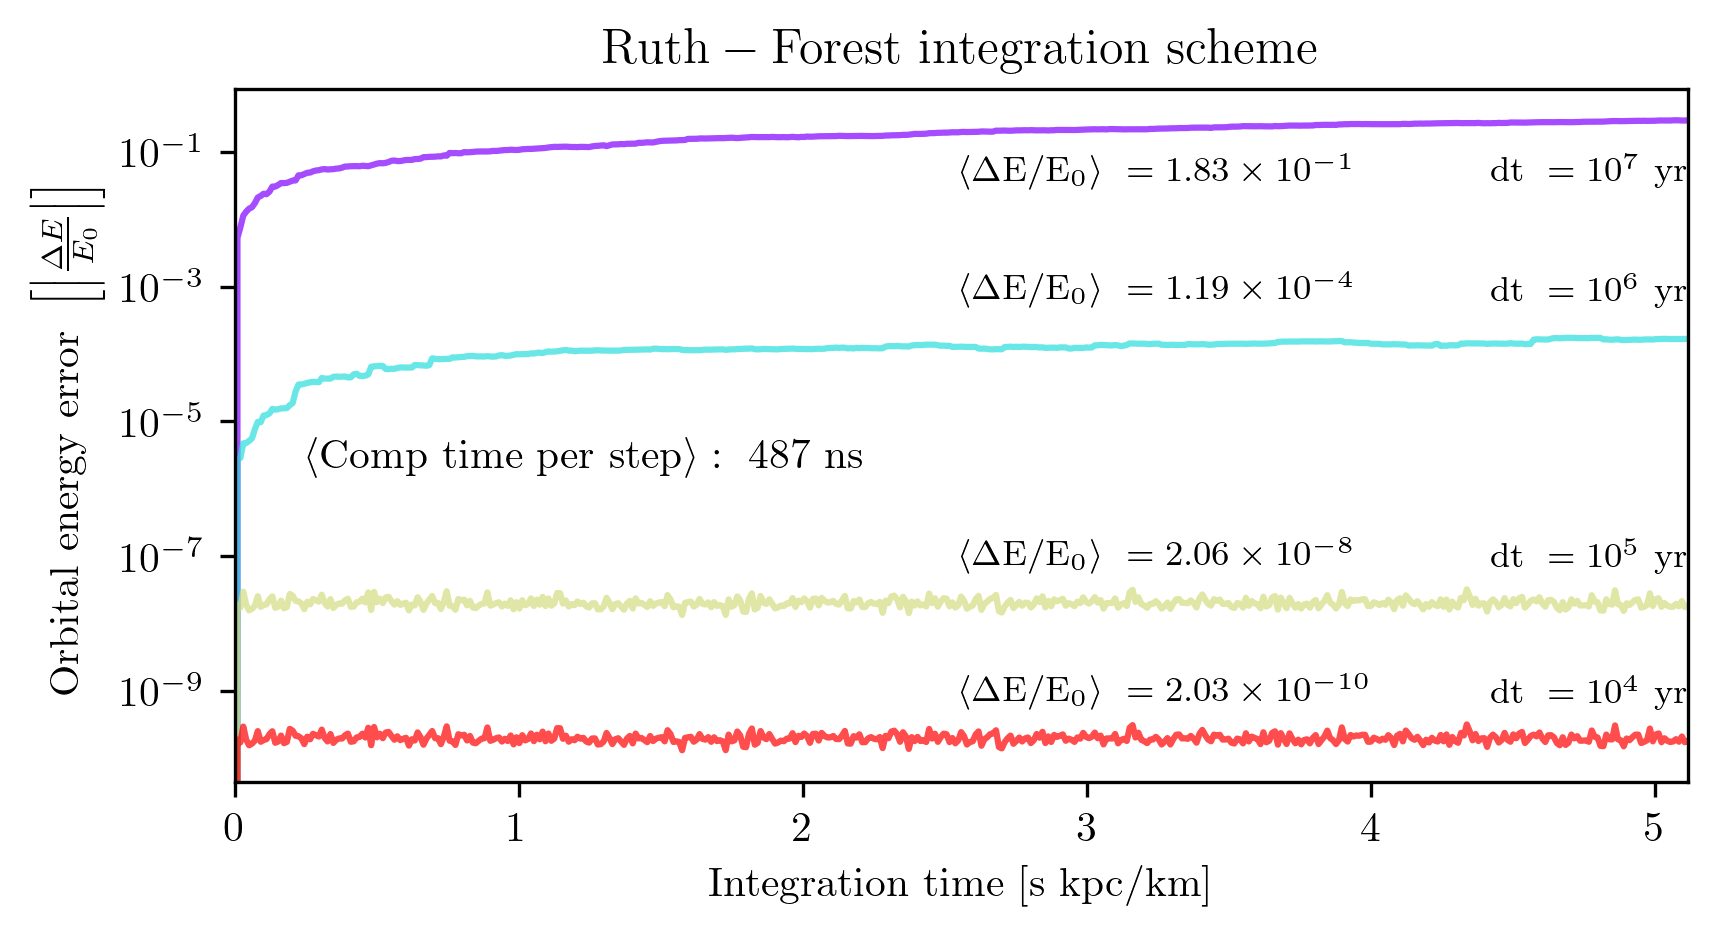
\includegraphics[width=\linewidth]{images/numericalErrorRuthForest.png}
            \caption{The conservation of energy error for the Ruth-Forest integration scheme for the globular cluster system. This plot is similar to Fig.~\ref{fig:numericalErrorLeapfrogVanilla}, but does not preesnt on the whole globular cluster system, just the average error in energy for the whole system with a given timestep. The timestep and time-average numerical error for the whole system is presented next to each curve. The average computation time per integration step per single object is as well.}
            \label{fig:numericalErrorRuthForest}
        \end{figure}
        Fig.~\ref{fig:numericalErrorMeanEnergyErrorRuthForestLeapfrog} compares the numerical error for again the total number of steps (which is inversely propertial to the timestep). It is clear that for a given step size, the Ruth-forest outperforms the Leapfrog, but is it actually better? To answer this question, I fit the two curves with their own trend lines to find the number of steps required to have a relative error of $10^{-8}$. With this requirement, The Leapfrog sceme requires 262,641 steps while the Ruth-Forest scheme requires 102,773 steps. However, given the difference in computation time per step, on average, the Forest-Ruth scheme takes $\sim 1.5$x more time for the same degree of numerical precision than the Leapfrog. For this reason, we use the Leapfrog algorithm. In this problem, numerical uncertainties are must less of a limiting factor compared to modeling uncertainties and observational uncertainties, so a better integrator for numerical precision is not worth the pay off of longer computation times. 
        \begin{figure}
            \centering
            \includegraphics[width=\linewidth]{images/numericalErrorMeanEnergyErrorRuthForestLeapfrog.png}
            \caption{The time averaged error in the conservation of energy for the entire globular cluster system for four different timesteps, for two different integration techinques: the Leapfrog against the Ruth-Forest. Their respective trend lines are shown.}
            \label{fig:numericalErrorMeanEnergyErrorRuthForestLeapfrog}
        \end{figure}

    \subsection{Star-particles in a static globular cluster}

        \begin{verbatim}
        VIDEO: cluster_showing_scale_and_dynamical_time.mp4
        \end{verbatim}
        
        A classic challenge in astronomy and the physical sciences arises when a problem involves two or more physical processes that operate on very different time scales. This is certainly the case when studying globular clusters. Figure~\ref{fig:GCsystemCharacteristicTimes} illustrates the orders-of-magnitude differences in time scales both across the globular cluster population and within individual clusters.

        \begin{figure}
            \centering
            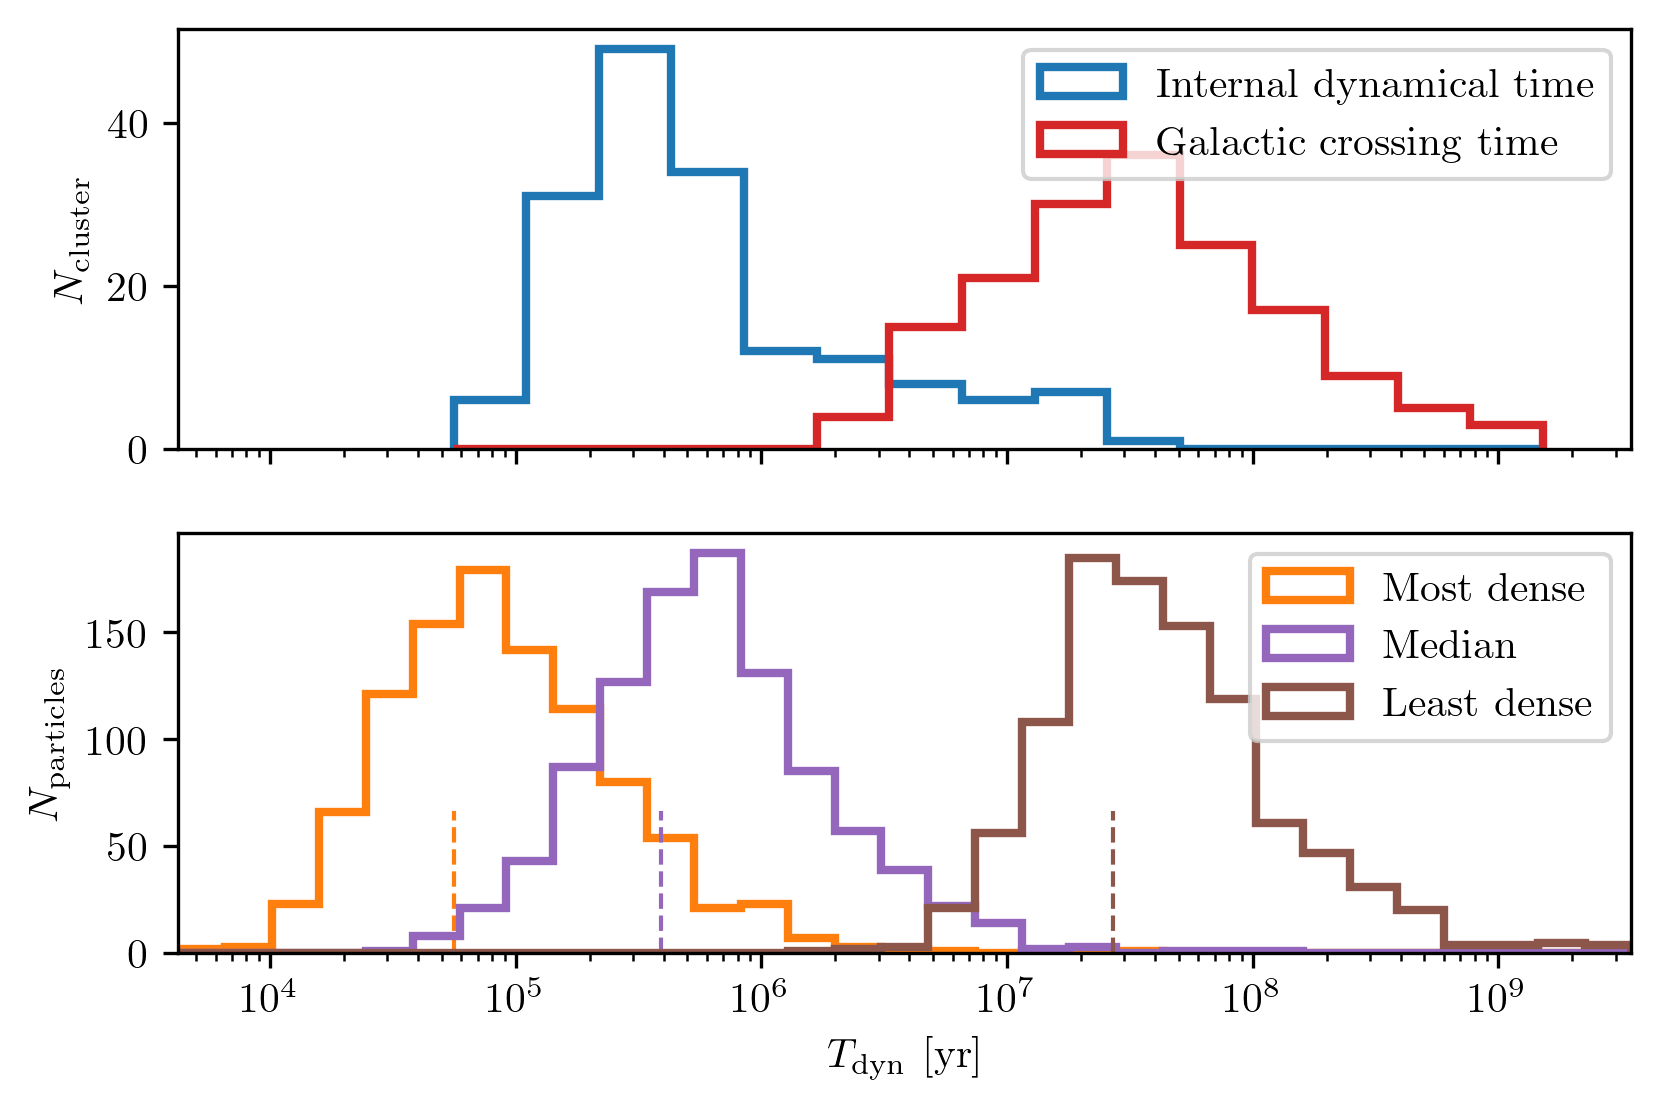
\includegraphics[width=\linewidth]{images/GCsystemCharacteristicTimes.png}
            \caption{The top panel shows orbital characteristic times of the globular cluster system, while the bottom panel shows internal characteristic times for three selected clusters. \textit{Top}: The red distribution shows the orbital crossing time of each cluster within the Galaxy, while the blue distribution shows a characteristic internal dynamical time. \textit{Bottom}: The distribution of crossing times for 1,000 sampled star particles within the globular clusters with the smallest, median, and largest internal dynamical times. The vertical dashed lines mark the characteristic internal dynamical times.}
            \label{fig:GCsystemCharacteristicTimes}
        \end{figure}

        A useful metric for characterizing a system's time scale is the \textit{crossing time}, which is the time it would take a star to reach the center of the system given its current speed:
        \begin{equation}
            t_\mathrm{cross} = \frac{r}{v}.
        \end{equation}
        While this quantity is not an integral of motion and varies as a star moves, it still provides a convenient and informative estimate of the dynamical time scale. It breaks down in extreme cases, such as a purely radial orbit near pericenter or apocenter where the instantaneous velocity approaches zero, but such cases are rare and do not undermine its utility. We compute the crossing time for each globular cluster in the galaxy (red distribution in the top panel of Fig.~\ref{fig:GCsystemCharacteristicTimes}) as well as for each individual star particle within the clusters.


        For the cluster as a whole, a robust characteristic dynamical time can be defined as:
        \begin{equation}
            \tau = \sqrt{\frac{a^3}{GM}},
        \end{equation}
        where \( a \) is a characteristic size of the system. This is often taken to be the half-mass radius. In this work, I adopt the half-mass radius rather than the Plummer scale radius, though the two are related by \( r_{\mathrm{1/2}} \approx 1.3a \). This time scale was computed for each cluster and is shown as the blue distribution in the top panel of Fig.~\ref{fig:GCsystemCharacteristicTimes}.

        Note that the distribution of cluster dynamical times has a long tail toward longer values, overlapping with the galactic crossing times. A natural question arises: could any cluster have a longer internal dynamical time than its orbital crossing time? The answer should be \textit{no}. If it takes longer for stars to orbit within the cluster than for the entire cluster to orbit the Galaxy, the cluster is effectively unbound or fully disrupted. I examined this question for the Galactic globular cluster population, and the results are shown in Fig.~\ref{fig:GCsystemStabilityDynamicalTimeRatios}. As expected, all clusters have internal dynamical times shorter than their orbital crossing times.

        Interestingly, the ratio of these two time scales serves as a useful diagnostic of cluster stability. Clusters in which stars complete hundreds or thousands of internal orbits per galactic orbit are significantly more stable than those where stars complete only a few. 
        \begin{figure}
            \centering
            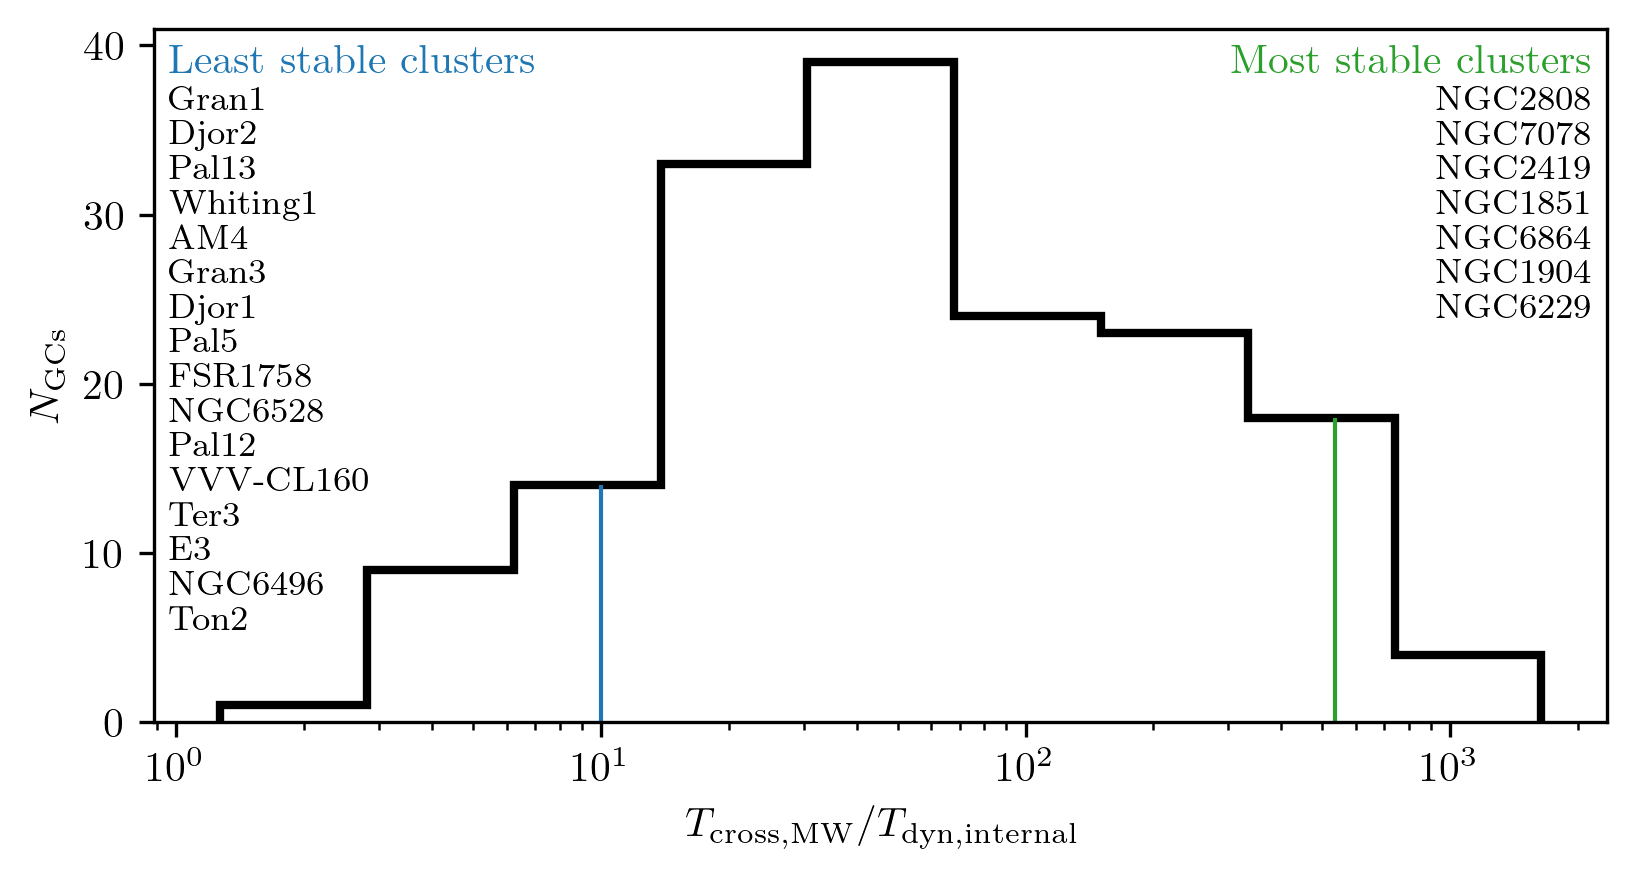
\includegraphics[width=\linewidth]{images/GCsystemStabilityDynamicalTimeRatios.png}
            \caption{Ratio of each globular cluster's galactic crossing time to its internal dynamical time (as shown individually in the top panel of Fig.~\ref{fig:GCsystemCharacteristicTimes}). Clusters whose internal dynamical times approach their galactic crossing times are near disruption. In contrast, denser clusters with much shorter internal times are more stable. The vertical bars indicate selected thresholds. Both lists rank clusters by increasing stability, with Gran~1 being the least stable and NGC~6229 the most.}
            \label{fig:GCsystemStabilityDynamicalTimeRatios}
        \end{figure}
        
        To properly compute the orbits of the star particles, the timestep must be small enough to resolve the orbit accurately while the star is inside the cluster. How should we choose this timestep? There are two criteria. The first is that the timestep should be some fraction of the cluster's dynamical time:
        \begin{equation}
            \Delta t' = \alpha ' \tau.
        \end{equation}
        I use a prime to indicate that this is a trial timestep, since the second criterion must also be satisfied: the total number of timesteps should be an integer, 
        \[
            N = \left\lceil \frac{T}{\alpha' \tau} \right\rceil,
        \]
        where $T$ is the total integration time. We round $N$ up to ensure a slightly smaller timestep, which becomes $\Delta t = T/N$. This also redefines the effective timestep fraction as $\alpha = \Delta t / \tau$.

        In the experiments presented in this section, I choose several fractions of each cluster's dynamical time and examine the resulting numerical errors. To efficiently explore a wide range of $\alpha$, I begin with a few trial values of $\alpha'$ and then round the number of steps down so that $N$ is not only an integer, but also a power of two. This leads to the following condition:
        \begin{equation}
            N = 2^{k-1}
        \end{equation}
        where $k \in \mathbb{N}$ is an integer index. The expression for $k$ becomes:
        \begin{equation} 
            k = \left\lceil \log_2\left(\frac{T}{\alpha '  \tau_\mathrm{dyn}}\right) + 1  \right\rceil.
            \label{eq:binary_time_step_criterion}
        \end{equation}
        
        The goal is now to determine the appropriate value of $\alpha$ to ensure energy conservation and time-reversibility. In the analysis presented in the previous sections, I selected timesteps without explicitly relating them to the crossing times of globular cluster orbits. Fig.~\ref{fig:numericalErrorLeapfrogVanilla} shows that a timestep of $\Delta t = 10^4~\mathrm{yr}$ achieves a mean relative energy error of $10^{-8}$. Meanwhile, Fig.~\ref{fig:numericalErrorReverseIntegration} shows that a timestep of $\Delta t = 10^5~\mathrm{yr}$ already achieves convergence in time-reversibility. Comparing these values to the typical crossing time shown in Fig.~\ref{fig:GCsystemCharacteristicTimes}, we find that they correspond to $\alpha$ values of approximately $2 \times 10^{-4}$ and $2 \times 10^{-3}$, respectively.

        In Fig.~\ref{fig:numericalErrorStaticPlummerSphereEnergyError}, I investigate energy conservation in a static Plummer sphere using trial values of $\alpha \in [10^{-4}, 10^{-3}, 10^{-2}, 10^{-1}, 1, 2]$. This experiment shows that values of $\alpha < 10^{-2}$ yield excellent energy conservation. In this section, we do not consider the time-reversability as the previous section has shown the integrations robustness with regard to this metric. However, this is our main metric for the next section.

        \begin{figure}
            \centering
            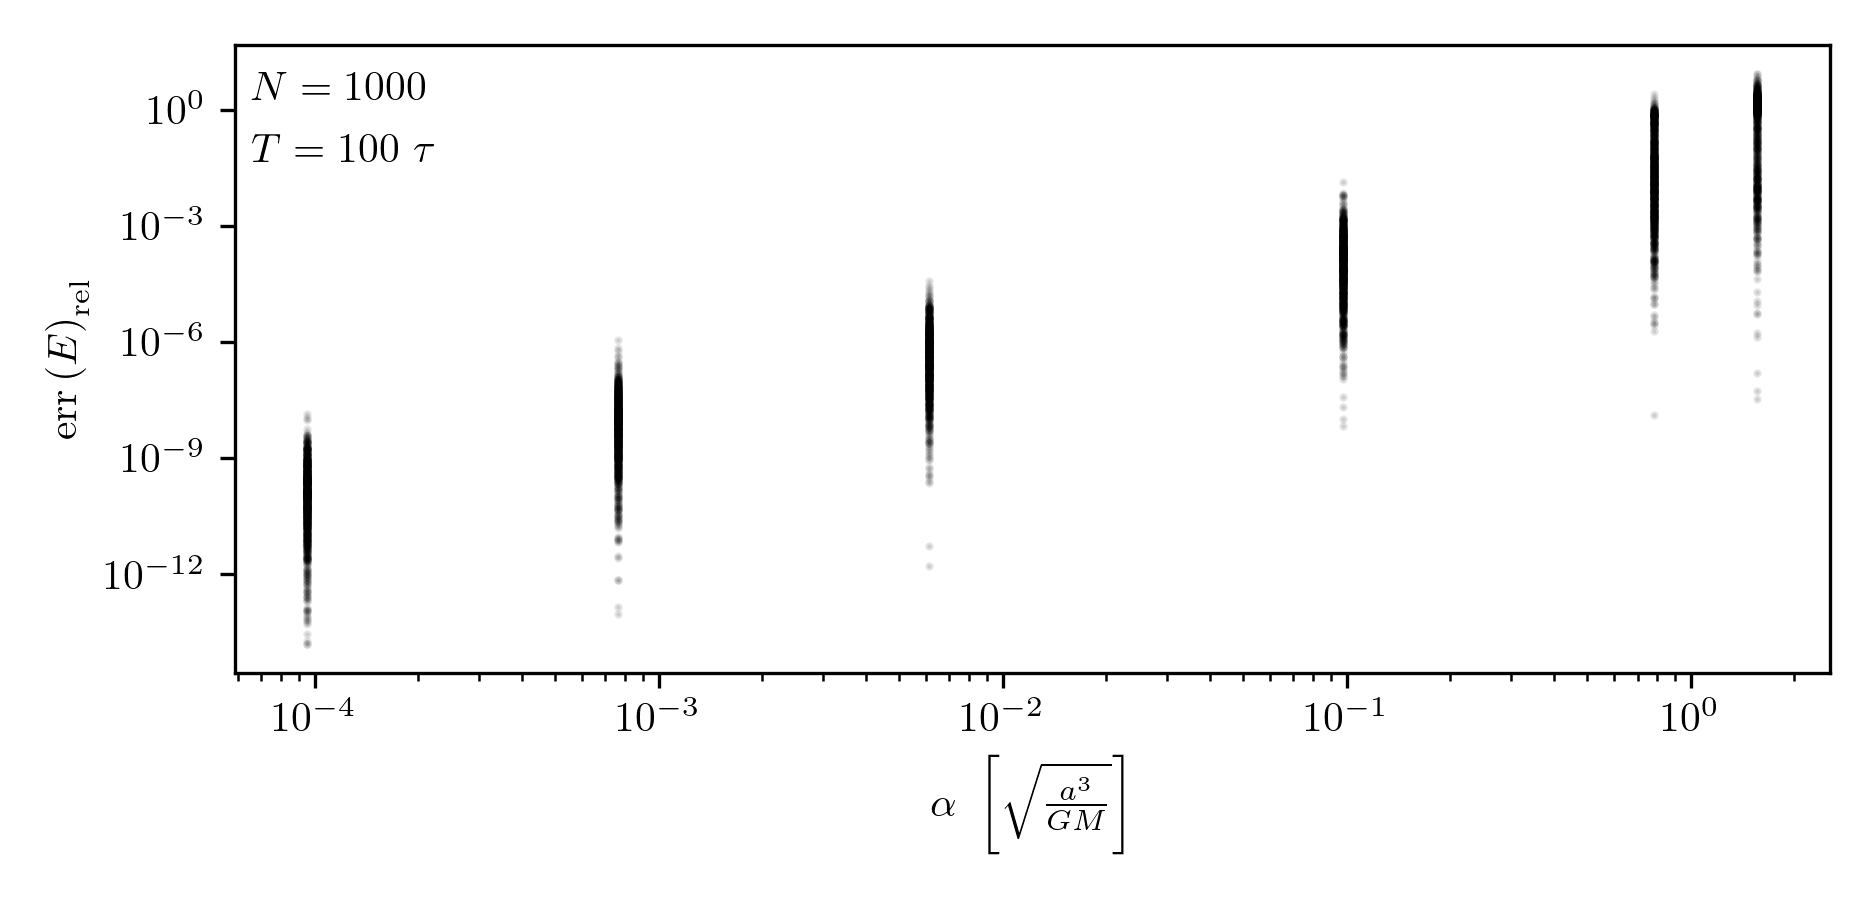
\includegraphics[width=\linewidth]{images/numericalErrorStaticPlummerSphereEnergyError.png}
            \caption{Relative energy error for a static Plummer sphere evolved with different timesteps. Each model contains the same number of particles, $N_p$, and is integrated for the same duration, $T$, as indicated on the plot. The x-axis shows the timestep size $\alpha$, defined as a fraction of the internal dynamical time $\tau = \sqrt{a^3 / GM}$.}
            \label{fig:numericalErrorStaticPlummerSphereEnergyError}
        \end{figure}

    \subsection{Full stream generation}
        The preceding sections assessed the numerical stability of integrating globular cluster orbits within the Milky Way, focusing on time-reversibility and relative energy error across two integration schemes: Leapfrog and Forest-Ruth. I also considered the computational cost associated with different temporal resolutions. Separately, I evaluated the energy conservation for star particles evolving within a stationary Plummer sphere, quantifying the relative error as a function of timestep. In that context, the cluster's potential was scaled to its scale radius, mass, and the gravitational constant. This non-dimensionalization allowed me to select timesteps as fractions of the internal dynamical time $\tau$ of each cluster. 

        In this section, I combine them: I examine the quality of orbit integration for star particles evolving within a globular cluster, which in turn is orbiting in the Galactic potential.

        I restrict the analysis here to the Leapfrog integrator for two main reasons. First, although the Forest-Ruth scheme achieves better energy conservation (see Fig.~\ref{fig:numericalErrorMeanEnergyErrorRuthForestLeapfrog}), this comes at a significantly higher computational cost, which outweighs its marginal gains for this application. Second, the equations of motion used to model stream generation require loading the position of the host cluster for each force computation. Because Forest-Ruth evaluates forces at non-uniform substeps, using it would require either: (1) storing and loading the cluster orbit at each substep, which would demand excessive disk space and complex code restructuring; or (2) interpolating the orbit at intermediate times, which introduces ambiguity regarding whether time-reversibility is preserved with linear or cubic interpolation. For these reasons, I opted not to explore Forest-Ruth further in the context of full stream generation.

        To assess the performance of the stream-generation method, I designed a quality assurance experiment, illustrated in Fig.~\ref{fig:NumericalErrorStreamRetrace_NGC6171}. I began by integrating the orbit of a globular cluster's center of mass backward in time by 1~Gyr. At that point, I initialized a Plummer sphere with 512 star particles using the cluster's half-mass radius and total mass. This system was translated to the center-of-mass phase-space coordinates and then integrated forward to the present day, forming a stream. I recorded the resulting positions and computation time. To test time-reversibility, I subsequently integrated the stream particles backward again for 1~Gyr.

        A note on terminology: although the cluster orbit is initialized from present-day observations, in the context of stream generation, I refer to the past position (1 Gyr ago) as the ``initial conditions''. The forward-integrated system represents the ``stream'', and the backward-integrated version of the stream is referred to as the ``retrace''.

        Fig.~\ref{fig:NumericalErrorStreamRetrace_NGC6171} shows the results for four different timesteps. As expected, increasing the timestep degrades time-reversibility. For the largest timestep ($\alpha \approx 1$, top left), the retrace fails to recover the original configuration. The retraced structure remains a stream and does not re-coalesce into a cluster. The results improve rapidly with decreasing timestep: at $\alpha \approx 2 \times 10^{-1}$, most particles return close to their starting positions with only slight offsets. At $\alpha \approx 2 \times 10^{-2}$, nearly all particles recover their initial conditions, and by $\alpha \approx 6 \times 10^{-3}$, the retrace is nearly perfect.

        \begin{figure}
            \centering
            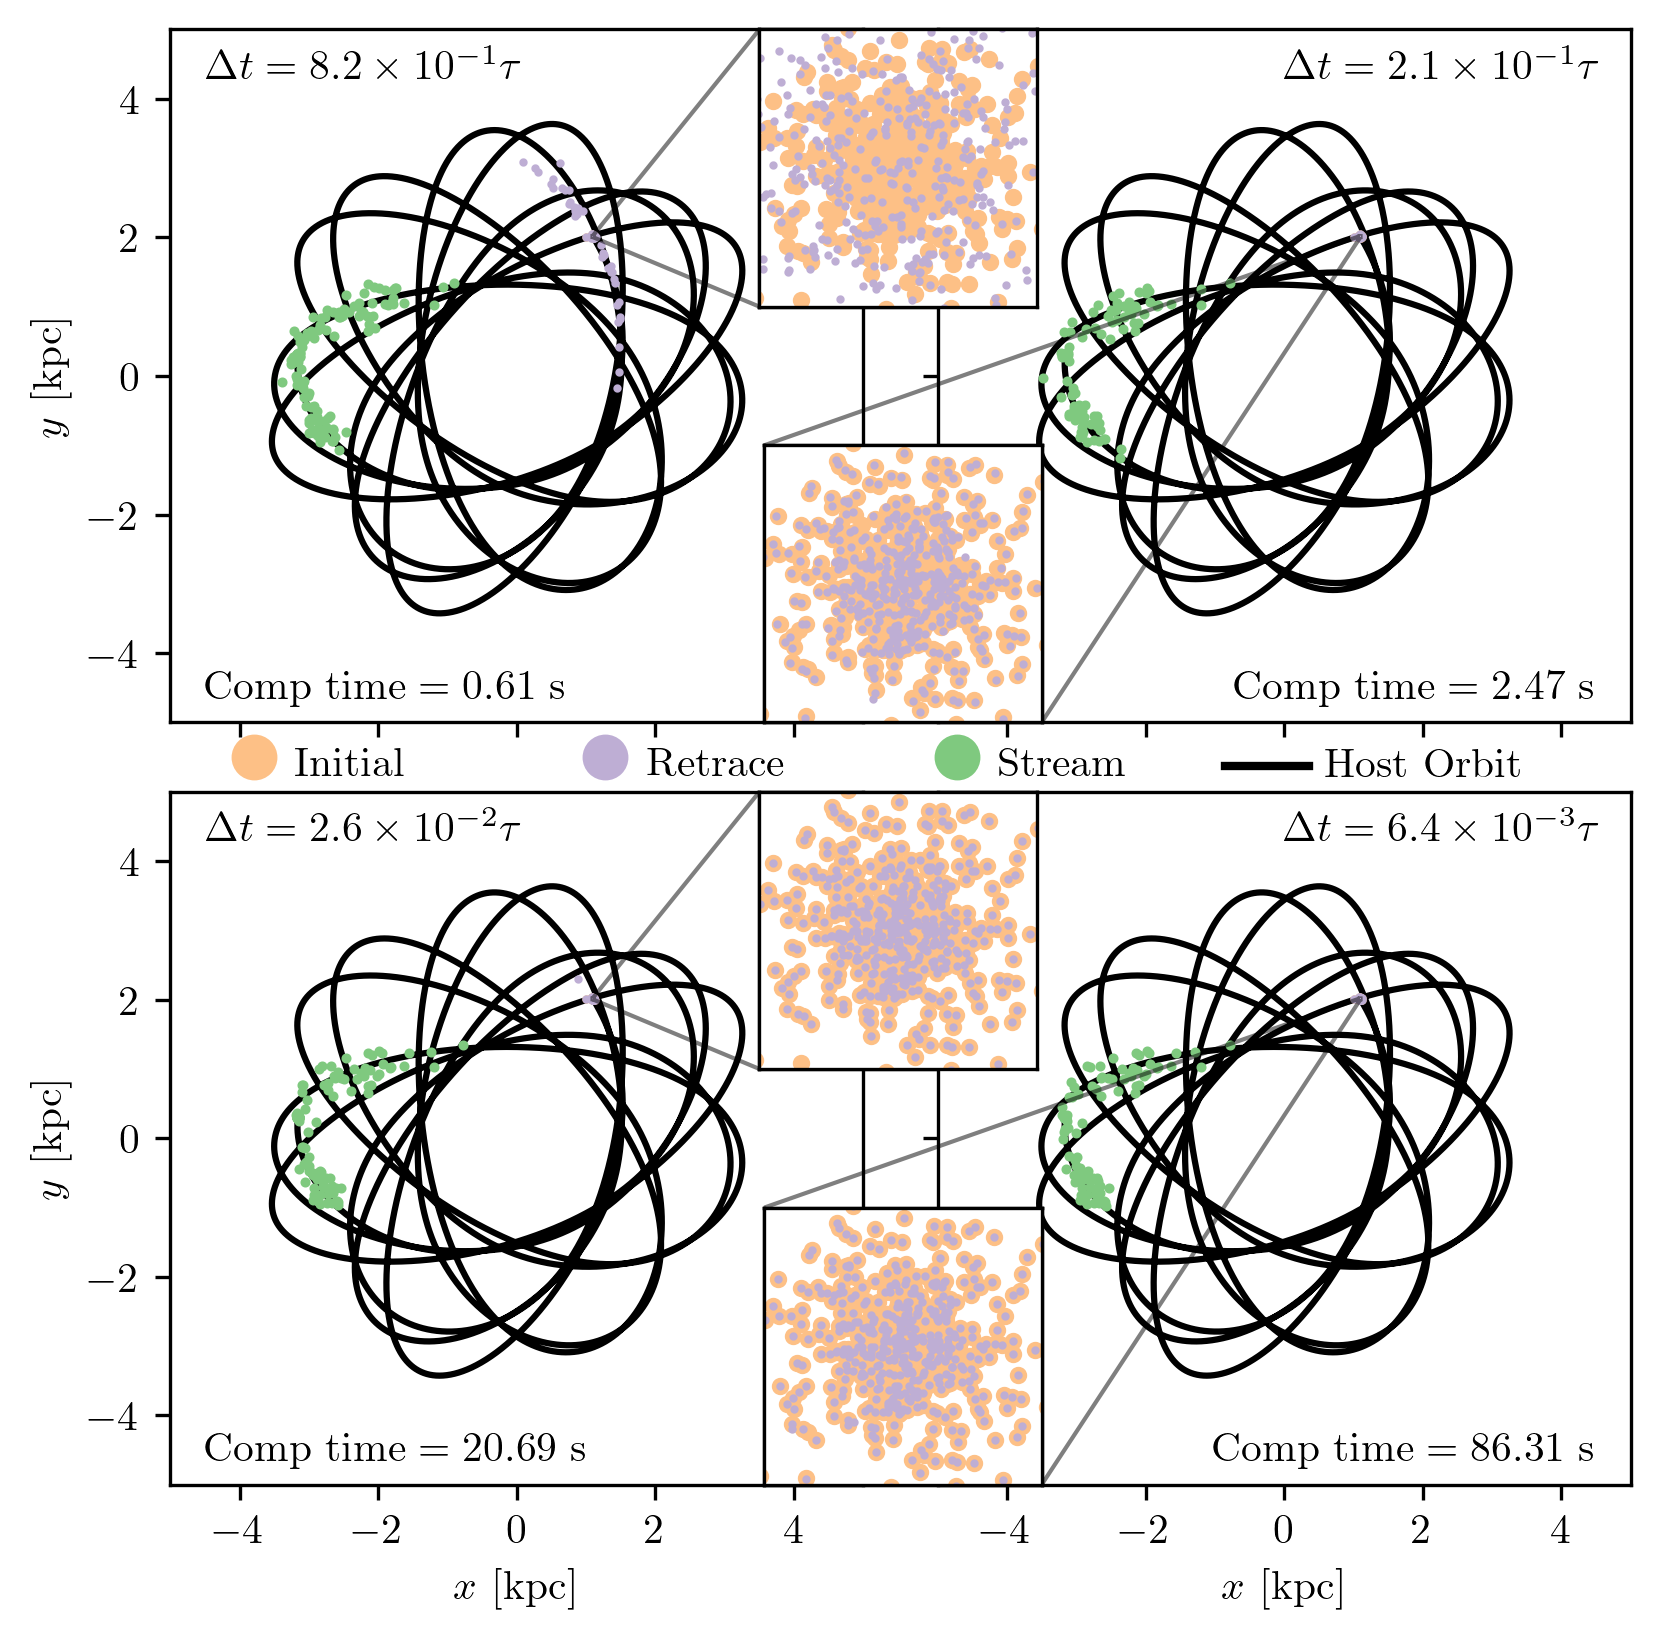
\includegraphics[width=\linewidth]{images/NumericalErrorStreamRetrace_NGC6171.png}
            \caption{Time-reversibility test for NGC~6171. The cluster's orbit was integrated backward by 1 Gyr, and a Plummer sphere of 512 particles was initialized at that position (``Initial''). The system was then integrated forward (``Stream'') and backward again (``Retrace''). Each panel shows a different timestep, which was selected as a fraction of the internal dynamical time $\tau$. The sub-panels zoom in on the cluster core, comparing the initial and retraced positions. Accuracy improves from top to bottom as the timestep decreases.}
            \label{fig:NumericalErrorStreamRetrace_NGC6171}
        \end{figure}

        Fig.~\ref{fig:NumericalErrorStreamRetrace_EnergyErrors} presents the integrator's energy conservation performance during the retrace phase of Fig.~\ref{fig:NumericalErrorStreamRetrace_NGC6171}, across the same timesteps.

        \begin{figure}
            \centering
            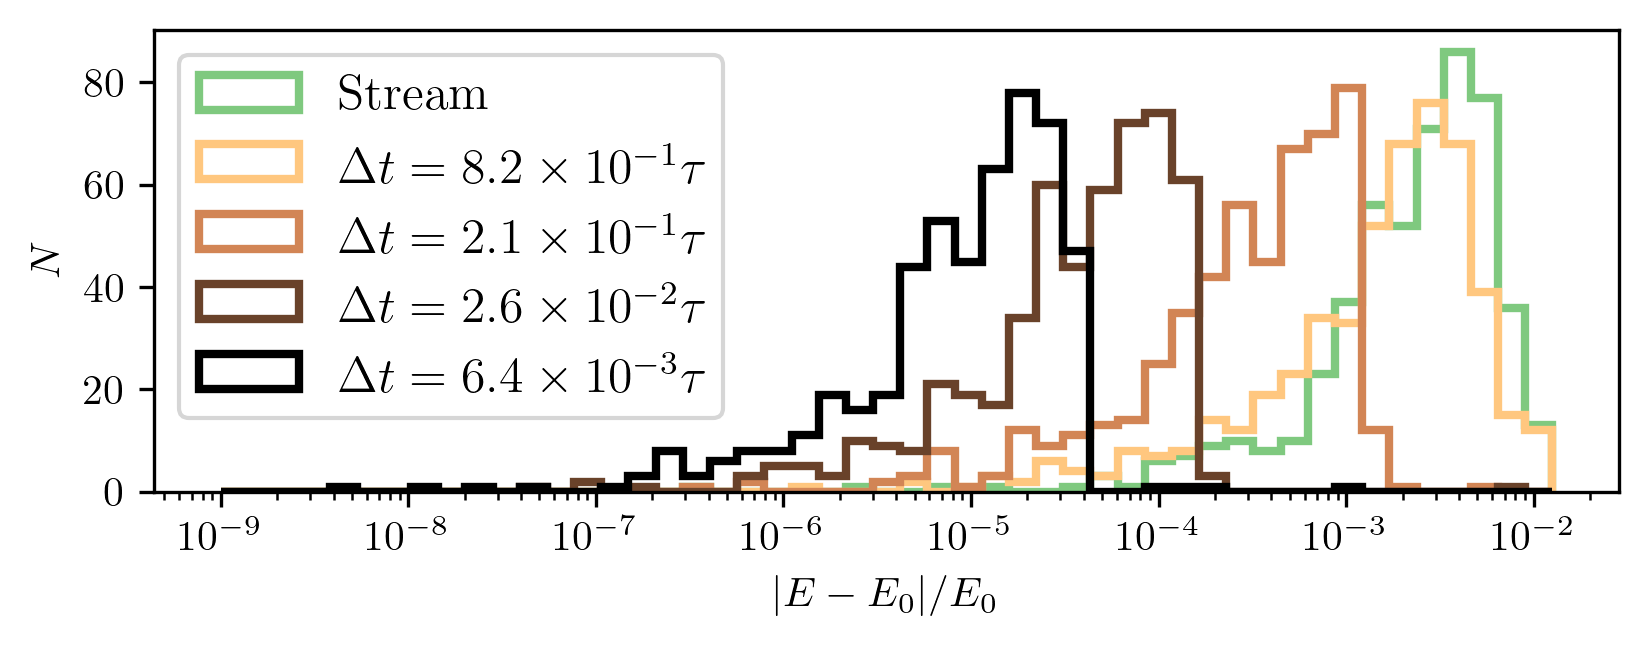
\includegraphics[width=\linewidth]{images/NumericalErrorStreamRetrace_EnergyErrors.png}
            \caption{Relative error in energy conservation during the retrace. As expected, accuracy improves with decreasing timestep. The \textit{stream} distribution shows the final energy of each particle relative to its initial energy and \textit{not} the quality of the integration. This reflects the spread in orbital energies imparted during initial sampling. At large timesteps, the retrace energy distribution approaches that of the stream.}
            \label{fig:NumericalErrorStreamRetrace_EnergyErrors}
        \end{figure}

        Although the retrace fails for the largest timestep in Fig.~\ref{fig:NumericalErrorStreamRetrace_NGC6171}, Fig.~\ref{fig:NumericalErrorStreamRetrace_EnergyErrors} shows that the relative energy error remains modest—between $10^{-4}$ and $10^{-2}$. However, this metric requires careful interpretation. What appears as an ``error'' primarily reflects the intrinsic spread in orbital energies among star particles, relative to the center-of-mass energy. 

        We can estimate this ratio by comparing the internal potential energy scale of the cluster to its orbital energy in the Galaxy. The cluster's characteristic potential is roughly $\Phi \sim GM/a$, with $M \sim 10^5~M_\odot$ and $a \sim 0.005$~kpc, giving $\Phi \sim 10^2~\mathrm{km}^2\,\mathrm{s}^{-2}$. Meanwhile, the typical orbital energy of a globular cluster is around $10^5~\mathrm{km}^2\,\mathrm{s}^{-2}$ (see Fig.~\ref{fig:energy_sensitivity_analysis_MWGCS_to_distance_RV_mu}). 

        This three-order-of-magnitude difference implies that the intrinsic energy spread from the Plummer sampling is about $10^{-3}$ of the total orbital energy, which is consistent with the the apparent energy ``error'' in the stream of Fig.~\ref{fig:NumericalErrorStreamRetrace_EnergyErrors}. Thus, this differences does not arise from numerical drift, but from the physical energy distribution encoded in the initial conditions. 

        Fig.~\ref{fig:NumericalErrorStreamRetrace_NGC6171} \& Fig.~\ref{fig:NumericalErrorStreamRetrace_EnergyErrors} demonstrate the case of a single cluster. How is the energy conservation for the entire catalog? Fig.~\ref{fig:NumericalErrorStreamRetraceEnergyConservation} presents the realtive error in the conservation of energy for retracing the orbit of each individual star particle per globular cluster for each cluster in the catalog. Each data point reports the mean error in the conservation of energy. Each cluster was integrated for 5~Gyr. The upper limits for the timesteps were sampeld logarithmically between $10^{0}$ and $10^{-2}$, the exact timesteps are based on the criterion from Eq.~\ref{eq:binary_time_step_criterion}.

        % From inspecting Fig.~\ref{fig:NumericalErrorStreamRetrace_NGC6171}, a timestep less than $3\times10^{-2}~\tau$ is great for retracing the orbit of each star particle and even $2\times10^{-1}~\tau$ suceeds in generally retracing the cluster. This would place the retrace energy conservation between $10^{-5}-10^{-3}$ on average per system. 
        \begin{figure}
            \centering 
            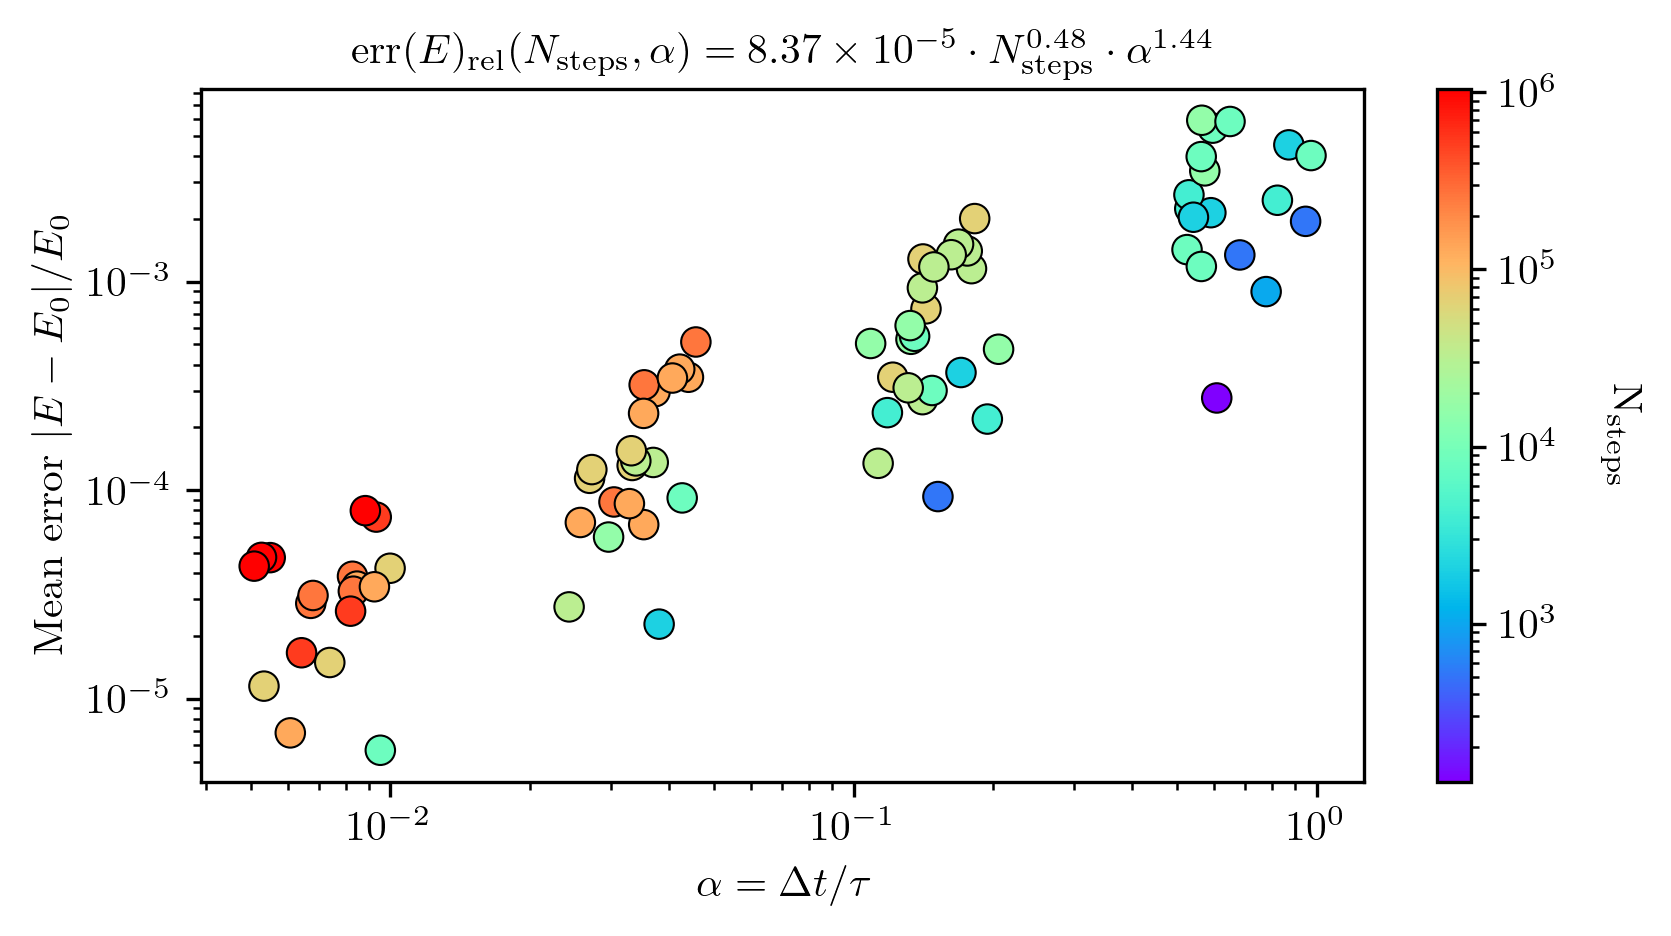
\includegraphics[width=\linewidth]{images/NumericalErrorStreamRetraceEnergyConservation.png}
            \caption{The conservation of energy for the retrace of each globular cluster in the catalog. Each cluster was sampled with 512 particles and integrated for 5~Gyr. Four upper thresholds for each timestep were logarithmically sampled between $10^{0}$ and $10^{-2}$, and selected individually for each cluster in combination with it's internal dynamical time that evenly divided the integration time. }
            \label{fig:NumericalErrorStreamRetraceEnergyConservation}
        \end{figure}

        The quality of the solutions is fundamental for proper results. However, computation time and cost is also very important. The main motivation in using the restricted three body problem was to save computation time. With N~body, the computation time should scale with $N_p^2$, while for the restricted three body problem it should scale with $N_p$. For both, it should scale linearly with the number of integration steps. 

        How does \texttt{tstrippy} perform? Fig.~\ref{fig:NumericalErrorComputationTimeScalingForStreams} presents an the results from an experiment with all the globular clusters, integrating them each for 1~Gyr. I choose the timestep to be at most 1/20 of each internal dynamical time, thus since each cluster has a different dynamical time, it will require a different number of steps. For each of these tests I use $10^1,~10^2,~10^2,~10^3$ particles and launched them on cluster at the paris observatory. Then, I fit a scaling law of $C(N_p,N_s) = \langle C\rangle N_p^a N_s^b$. If the code scales linearly, then each exponent, $a,~b$, should be 1 and $\langle C\rangle$ would be the mean computation time. 
        
        Fig~\ref{fig:NumericalErrorComputationTimeScalingForStreams} shows that the code is \textit{less} efficient than linear scaling with number of particles, since the best fit exponent is $1.35$. However, it scales \textit{better} than linear with the number of steps. Perhaps this can be explained by the fact that there is overhead time involved for initiating and ending each simulation. As the number of steps increases the fixed overhead proportionally takes up less of the total time. Since the power law has an exponent of $0.95$, the overhead is marginal. However, it is fortunate that the exponent is not greater than 1, which would mean the code would slow down with execution time. 
        \begin{figure}
            \centering
            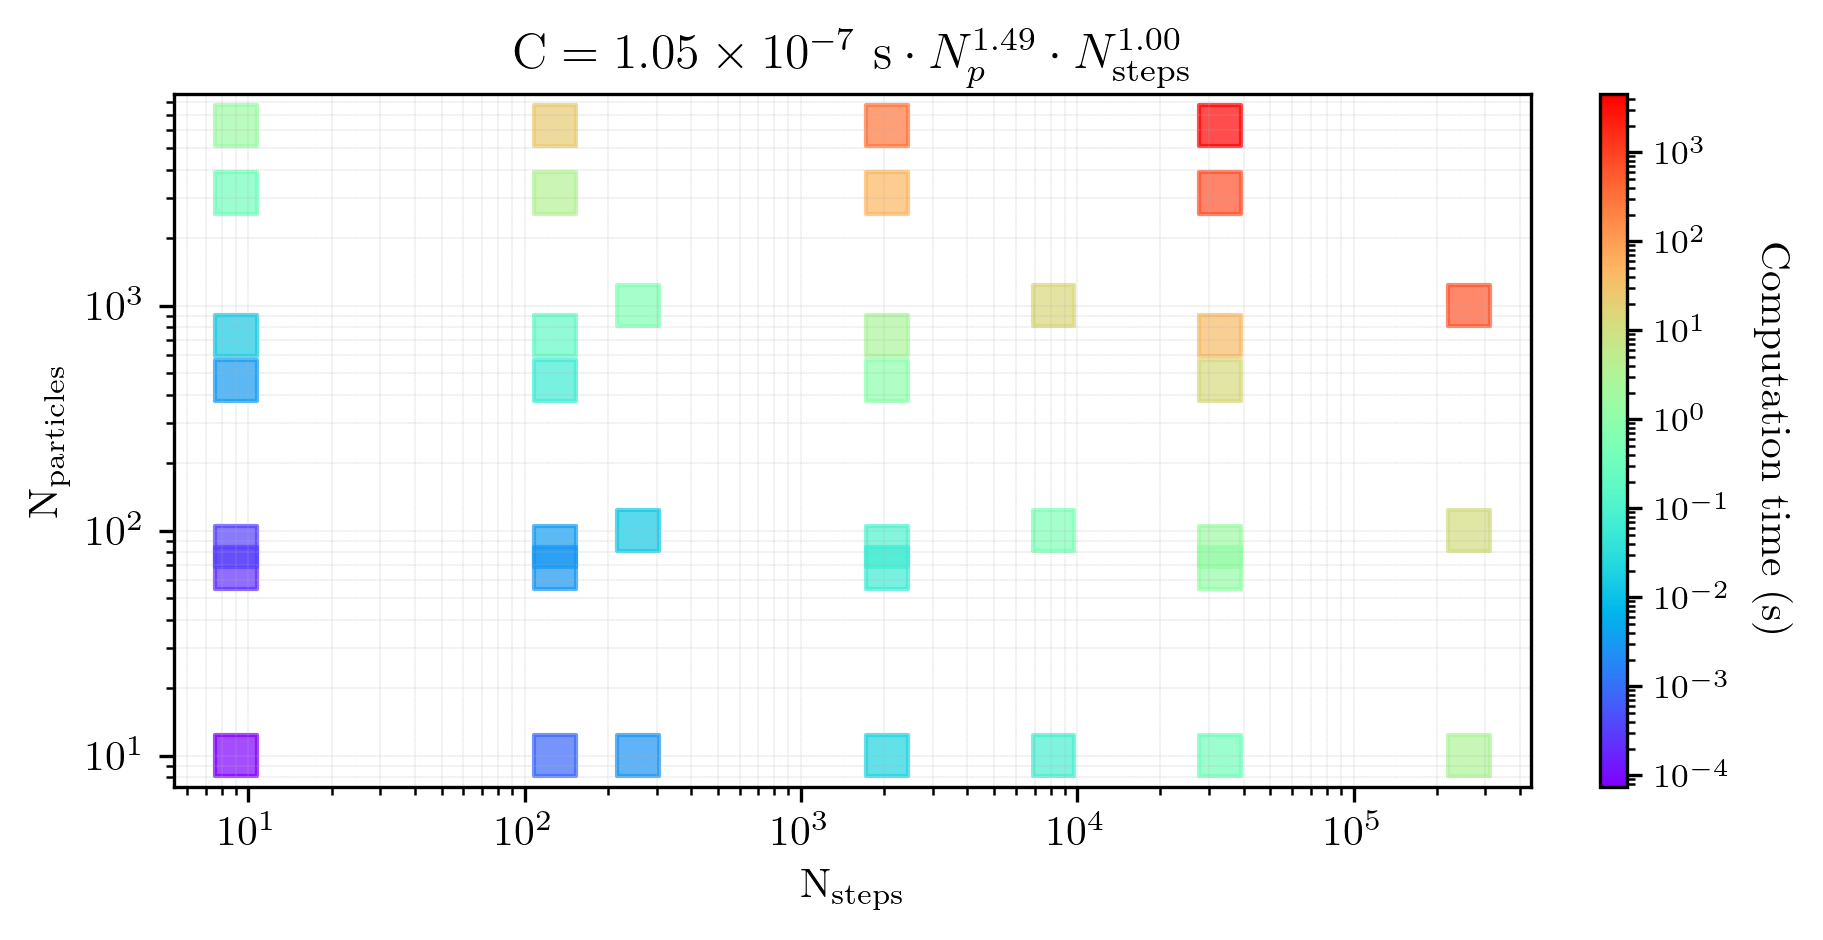
\includegraphics[width=\linewidth]{images/NumericalErrorComputationTimeScalingForStreams.png}
            \caption{How the computation scale time scales with the number of particles and the number of steps taken.}
            \label{fig:NumericalErrorComputationTimeScalingForStreams}
        \end{figure}
        Putting Fig.~\ref{fig:NumericalErrorStreamRetraceEnergyConservation} and Fig.~\ref{fig:NumericalErrorComputationTimeScalingForStreams} together, we get can estimate for how long it completes to run these simulations. If we want all simualtions to have error better relative error on the retraced conservation of energy than about 10$^{-3}$, then we must pick timesteps that are smaller than about 1/20 of the dynamical time. With this criteria selected, we can compute the number of timesteps necessary for each globular cluster, which is a function of it's internal dynamical time. By doing so, I find that the fastest cluster can be computed in $\sim$~30~minutes. The median computation time is $\sim$17~hours. The largest computation time was $\sim$~5~days. The total CPU time for the whole catalog is $\sim$~194~days. 

        \subsubsection{A note on non-symplectic integration}

        During the writing of this thesis, I discovered a bug in my code that affected the integration scheme. Specifically, the error concerned the way I handled the host orbit during the integration of the star particles. In earlier implementations, I would integrate the orbit of the host using the same timestep that I used later to integrate the orbits of the star particles. However, this approach violated the structure of the Leapfrog integration scheme.

        In Hamiltonian integration, it is essential that the drift and kick steps alternate in a consistent manner. Since I implemented a \textit{drift}-\textit{kick}-\textit{drift} (DKD) scheme, the kicks occur at the midpoint of each timestep, meaning that forces should be evaluated at intermediate positions. Previously, I erroneously computed the relative position vector as
        \[
        \Delta \vec{r}_i = \vec{r}_{p,i+1/2} - \vec{r}_\mathrm{GC,i},
        \]
        instead of the correct expression:
        \[
        \Delta \vec{r}_i = \vec{r}_{p,i+1/2} - \vec{r}_\mathrm{GC,i+1/2}.
        \]

        This mistake appeared in both \citet{2023A&A...673A..44F} and \citet{2025A&A...699A.289F}. Does this invalidate our results? To assess the impact, we can compare Figs.~\ref{fig:NumericalErrorStreamRetrace_Pal5_Nsteps_32768_stepsPerTau_420} and \ref{fig:NumericalErrorStreamRetrace_NGC6171_Nsteps_1048576_stepsPerTau_311}. In Fig.~\ref{fig:NumericalErrorStreamRetrace_Pal5_Nsteps_32768_stepsPerTau_420}, the same retracing experiment was performed, but using the flawed integration: the host orbit was only provided at the same grid points as the stream. In the left panel, we see that the globular cluster does not perfectly re-coalesce when integrating backward in time, but the result is not catastrophic. Physically, we do not expect this process to be perfectly time-reversible; however, such irreversibility should ideally arise from physical modeling, not from numerical artifacts.

        We also observe that the distribution of the relative error in energy conservation is nearly identical between the retraced and the original stream. In any case, once the stars move beyond the Jacobi radius, their dynamics are dominated by the galactic potential. Since this potential was integrated correctly and symplectically, the orbits of stars outside the cluster remain reliable and physically meaningful.

        \begin{figure}
            \centering
            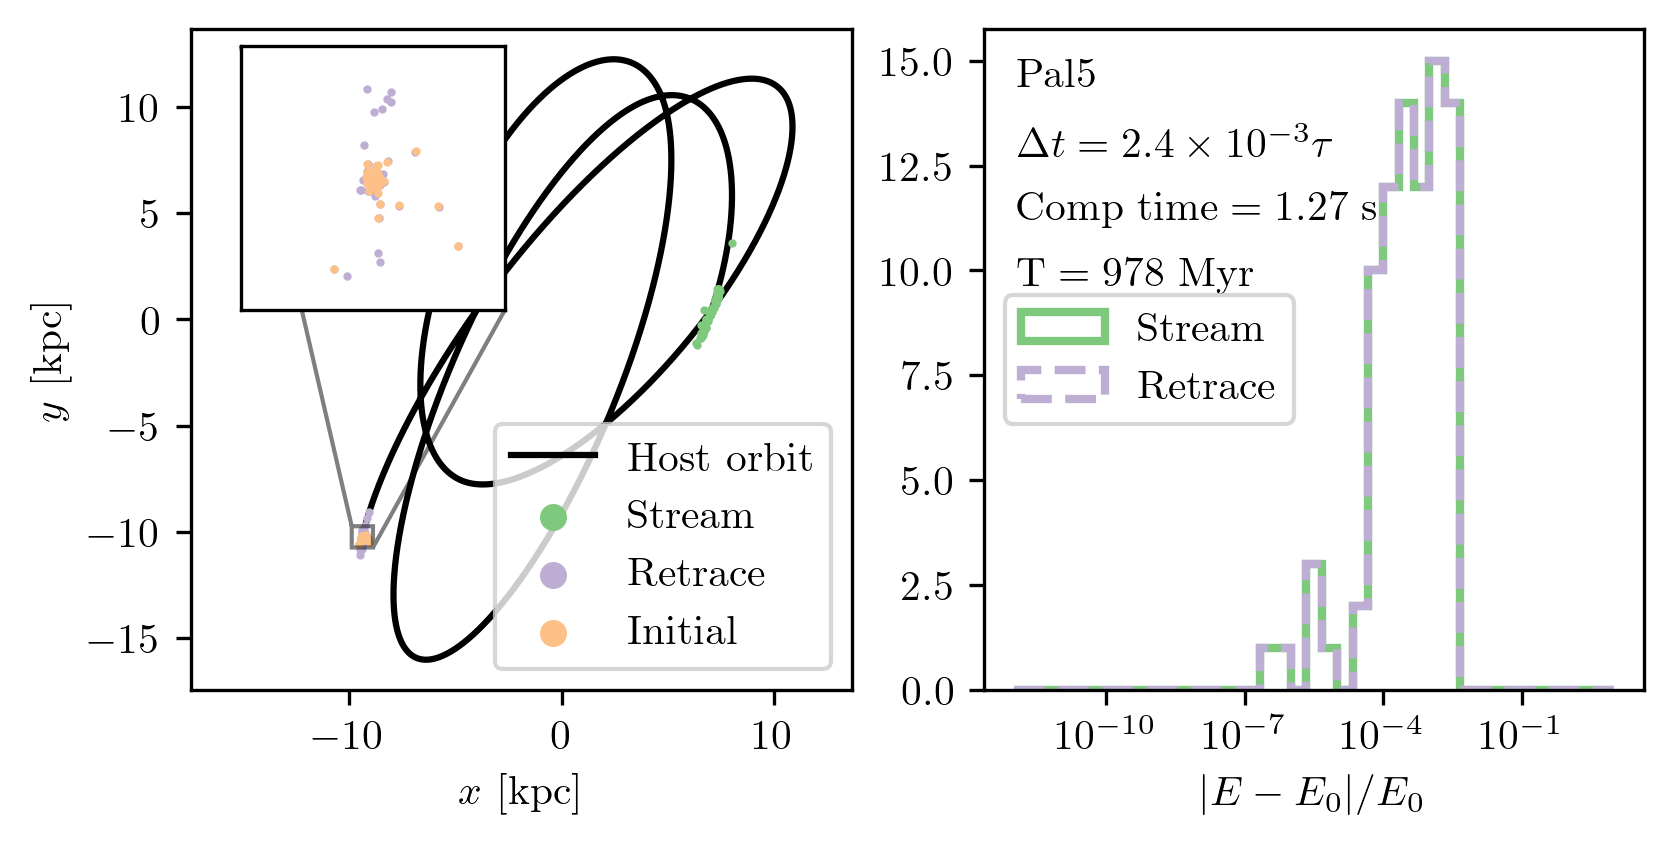
\includegraphics[width=\linewidth]{images/NumericalErrorStreamRetrace_Pal5_Nsteps_32768_stepsPerTau_420.png}
            \caption{An illustration of how an incorrect integration scheme breaks time reversibility. The center of mass of Palomar~5 was integrated backward in time by 1~$\mathrm{s}~\frac{\mathrm{kpc}}{\mathrm{km}}$. A Plummer sphere with 464 particles was sampled around this position (labeled “Initial”), then integrated forward to produce the “Stream.” The right panel shows the distribution of relative energy error. The stream was then integrated backward in time by the same amount, resulting in the “Retrace” configuration. The timestep was chosen as a fraction of the internal dynamical time scale, $\tau$.}
            \label{fig:NumericalErrorStreamRetrace_Pal5_Nsteps_32768_stepsPerTau_420}
        \end{figure}
        As a result of this discovery, I updated the \texttt{tstrippy} code to warn users if the host orbit is not sampled at $2N + 1$ points, where $N$ is the number of integration steps. While the flawed implementation breaks strict symplecticity for the internal cluster dynamics, the Leapfrog integration for the globular cluster orbits was still used correctly. This ensures that the cluster center of mass returns to its present-day sky position and that stars outside the cluster follow accurate galactic orbits. Ultimately, the simplification of using a static Plummer sphere—whose mass and size remain fixed—is a greater limitation than this particular numerical error.

        Lastly, I discovered this error while writing about the Forest-Ruth integration method. To implement this scheme correctly, I would need to know the position of the globular cluster's center of mass at four intermediate points across two timesteps, with the spacing determined by the coefficients in Table~\ref{tab:forest_ruth_coeffs}. This would require either storing additional mini-time-step data or interpolating the globular cluster's trajectory between saved snapshots. Both options would necessitate a substantial refactoring of the code or an impractical increase in memory usage per orbit. Given the results shown in Fig.~\ref{fig:numericalErrorMeanEnergyErrorRuthForestLeapfrog}, the gain in accuracy does not justify the computational cost.


\section{Tstrippy}

    Developing my own package gave me a deeper understanding of code structure, numerical algorithms, and the subtleties of scientific programming. It also gave me the confidence to later use other packages more effectively. The \texttt{tstrippy} code is available on GitHub and runs on macOS and Linux.

    \begin{itemize}
        \item How does \texttt{tstrippy} actually work?
        \item f2py? 
        \item setuptools $\rightarrow$ meson 
        \item incompatbile with old mac processors and being blocked at numpy 1.23 until the meson migration 
        \item f2py, and why did we choose to use Fortran? 
        \item Bovy's guide for making a public python package
        \item a brief overview of how it works. 
        \item how I can either save orbits or snapshots
        \item some notes on parallelization
    \end{itemize}

    Since all star-particles are independent from one another, they can be parallelized. This is \textit{data}-parallelization, where the same job is being performed but the input data is changed. This is a much easier paradigm compared to \textit{task}-parallelization different processors do different things to do the data and may need to communicate with one another. In this experiment, since I am simulating the whole globular cluster catalog and sampling the orbital uncertainties with monte-carlo, as explained in Chapter~5, I often times parallelize over different clusters. 
            
    However, if I want to accelerate one particular computation, then I must split the number of particles into batches. If I run small simulations on my personal computer, I can take the total number of particles and divide by the number of desired batches. Usually, I divide into the number of processors that I am going to use. $N_\mathrm{per~batch}=N_p//N_\mathrm{batches}$. However, I need to integer divide because the number of particles needs to be an integer. Then, with the last batch, I add the remaining particles, which is $N_\mathrm{left over} = N_p - N_\mathrm{batches} \times N_\mathrm{per~batch}$. 





\chapter{Tidal}
\section{General intro}

How should I introduce this paper??

\section{\bf{Numerical method}}\label{methods}

    To model the formation and evolution of extra-tidal features around Galactic globular clusters, we use a set of codes, called Globular Clusters' Tidal Tails (GCsTT)  developed by our group. It comprises two python codes, for the backward and forward integration of a stellar system, made of N test-particles (see Sect.~\ref{numerical}). These codes are separated for data organization and management, while the (computationally) most expensive part, namely, the calculation of the accelerations acting on the N particles and the orbits integration, is realized by means of a Fortran module written by our group. This module is interfaced to python by means of f2py directives from NumPy. The use of test-particle methods for modeling the tidal stripping process is widespread in the literature, where these methods are  usually applied to one or few clusters at a time \citep[see, e.g., ][]{lane12, mastrobuono12, palau19, piatti21a, grillmair22}. In this work, we apply a test-particle methodology to the whole set (159) of Galactic globular clusters for which this is currently possible, also taking into account, for each cluster, the errors on astrometry, line-of-sight velocities\footnote{Note: the term ``line-of-sight velocities''  adopted in this paper corresponds to the term ``radial velocities'' often used in the literature, as well as in the Gaia catalogues. We prefer the use of the first term, since the second is usually used also to indicate the (Galactocentric) radial velocities and can introduce some ambiguity, especially when different coordinate systems are used. We emphasize that the choice to use the term ``line-of-sight velocity'' is not new \citep[see, e.g., ][]{vasiliev21}.} and distances. In the following, we describe the two main steps of the procedure used by GCsTT  to simulate the tidal stripping process (Sect.~\ref{numerical}), the initial conditions adopted for the clusters' parameters and their mass distribution (Sect.~\ref{initialconds}), as well as the Galactic potentials (Sect.~\ref{galmod}).
    \subsection{Simulations of the tidal stripping process:  Two-step procedure}\label{numerical}
        To model the formation and evolution of extra-tidal features around Galactic globular clusters, and predict their current properties, we proceed as follows: 

        \textit{Step i: Backward integration. Reconstructing the globular cluster orbit over the last 5~Gyr}: First, for each Galactic globular cluster for which the distances from the Sun, proper motions, line-of-sight velocities, and structural parameters are  available (see Sect.~\ref{initialconds}), we determine their current positions and velocities in a Galactocentric reference frame, in which the Sun is at $(x_\odot, y_\odot, z_\odot) = (-8.34, 0., 0.027)$~kpc \citep{chen01, reid14} and at a given velocity for the local standard of rest, $v_{LSR}= 240$~km/s \citep{reid14}, and a peculiar velocity of the Sun with respect to the LSR, $(U_{\odot}, V_{\odot}, W_{\odot})  = (11.1, 12.24, 7.25)$~km/s \citep{schonrich10}. We then integrate the orbit of a single point mass, representing the cluster barycenter, backwards in time for 5~Gyr, and in this way, we retrieve its position and velocity at that time in the chosen Galactic potential (see Sect.~\ref{galmod}). We notice that other choices for the Sun's position or velocity with respect to the Galactocentric frame would have been possible. For example, \citet{piatti21a} adopted the same values as ours for the $v_{LSR}$ and for the peculiar velocity of the Sun but with a different distance to the Galactic center \citep[8.1~kpc in their work, see][]{gravity18}. The difference in the adopted position of the Sun is, however, generally smaller than the uncertainties affecting our knowledge of the distance of Galactic globular clusters to the Sun. For this reason, we do not to explore the dependency of the results presented in this paper with regard to these choices. 

        \textit{Step ii: Forward integration. Test-particle streams from the past to the present day}: Once the positions and velocities of the barycenter of each cluster, 5~Gyr ago, have been determined, we build  the corresponding $N$-body system, with N = 100 000 particles.  The phase-space coordinates of these particles are generated following a Plummer distribution, with the total mass and half-mass radius as described in Sect.~\ref{initialconds}. The barycenter of this $N$-body cluster is then assigned initial positions and velocities in the Galactic model, as those retrieved at step $(i),$ and the cluster is then integrated forward in time until the present day. Particles in this $N$-body system are modeled as test-particles, that is, they experience the gravitational field exerted by the globular cluster itself (see Sect.~\ref{initialconds}) and by the Galaxy (see Sect.~\ref{galmod}), but do not generate any gravitational field themselves. This allows us to maintain a computational time which scales as $O(N)$ and not as $O(N^2)$, as would be the case for a direct $N$-body self-consistent computation.

        In the following, we refer to these simulations, made by using the most probable values on distances, proper motions, and line-of-sight velocities, as the ``reference simulations.'' In addition, for each globular cluster, we also take into account the errors on its distance, proper motions, and line-of-sight velocity,  assuming Gaussian distributions of the errors, treated independently, and by generating 50 random realizations of these parameters.  For each of these realizations, we repeat the steps  described above, that is: (\textit{step i}) we determine the associated current positions and velocities in the chosen Galactocentric reference frame, we integrate the orbit of the single-point mass (representing the cluster barycenter) backwards in time, retrieving the corresponding values 5~Gyr ago, (\textit{step ii}) we build an $N$-body cluster containing $N$= 100~000 particles, with total mass and half-mass radius as those used for the reference simulation, and then we integrate the $N$-body cluster forwards in time until the present-day position. 

        To summarize, for a given Galactic potential, we run $159\times (50+1)=8109$ simulations, where 159 is the total number of clusters for which we currently have both 6D phase-space information and structural parameters. As we discuss in the following section, the whole set of globular clusters has been evolved in three different Galactic potentials, which implies that a total of 24 327 simulations have been run.

        For the orbit integration, a leap-frog algorithm is used, with a fixed time-step, $\Delta t$, and a total number of steps, $N_{steps}$, such that the total simulated time is  $\Delta t \times N_{steps}=5$~Gyr. The choice of the value of $\Delta t$ adopted to simulate each cluster in the Galactic potential has been based on the energy conservation of the corresponding cluster evolved in isolation (i.e., without the effect of the Galactic gravitational field for 5~Gyr). For the majority of the clusters (109/159), this value was set to $\Delta t = 10^5$~yr (for a corresponding value of $N_{steps}=50\,000$), while for the remaining clusters (50/159) a  $\Delta t = 10^4$~yr (for a corresponding value of $N_{steps}=500\,000$) was used. We refer to Appendix~\ref{deltat} (and in particular to Table~\ref{tcross-energy}) for additional details on the choice of $\Delta t$ for the whole set of clusters. As for the total simulated time, while globular clusters are much older than 5~Gyr, we chose this time limit because the longer back in time we could go, the less certain we would be of the Galactic environment. In addition, the last significant mergers in the Galaxy happened between 9 and 11~Gyr ago  \citep[see][]{belokurov18, helmi18, dimatteo19, gallart19, kruijssen20} -- well before the time interval simulated in this study. Other more recent interactions, such as the accretion of Sagittarius and of the Magellanic Clouds, may perturb the Galactic potential as well \citep[see, e.g.,][]{vasiliev21b} and we plan to investigate their impact on the properties of globular cluster streams in the future.

        For each realization, we generate an output file in an hdf5 format\footnote{\url{https://www.hdfgroup.org/solutions/hdf5/}} containing the values for the right ascension ($\alpha$), declination ($\delta$), distance from the Sun ($D$), along with the components for proper motion in the equatorial coordinate system ($\rm \mu_{\alpha}\cos(\delta)$ and $\rm \mu_\delta$), the line-of-sight velocity ($\rm v_{\ell os}$), longitude ($\ell$), latitude ($ b$), as well as the components for proper motion in the Galactic coordinate system ($\rm \mu_{\ell}\cos(\mathit{b})$ and $\rm \mu_b$) and the Galactocentric positions ($x, y, z$), velocities ($v_x, v_y, v_z$) and energy, $E$, of each particle in the simulated system. We used Astropy \citep{astropy13, astropy18} to convert the Galactocentric positions and velocities in the equatorial and Galactic quantities $\alpha, \delta, D, \rm \mu_{\alpha}\cos(\delta), \rm \mu_\delta, \rm v_{\ell os}, \ell, b, \rm \mu_{\ell}\cos(\mathit{b})$, and $\rm \mu_b$.

        For each particle, we also save its escape time $t_{\rm esc}$,  defined as the time at which the particle escapes from the cluster, that is, the time, $t,$ at which the particle satisfies the relation\footnote{If the particle is gravitationally bound to the cluster until the end of the simulation, $t_{\rm esc}$ is set equal to $-9999$.}:
        \begin{equation}
            E_{GC}= 0.5 \times \left( (v_x-v_{x, GC})^2+(v_y-v_{y,GC})^2+(v_z-v_{z,GC})^2\right)+\Phi_{GC} > 0,
        \end{equation}
        with $E_{GC}$ being the total specific energy of the particle relative to the cluster, that is, the sum of the potential energy, $\Phi_{GC}$, due to the gravitational field of the cluster (see Eq.~\ref{gcpot}), and of the kinetic energy, relative to the cluster barycenter, $T_{GC}=0.5 \times \left( \left(v_x-v_{x, GC}\right)^2+\left(vy-v_{y,GC}\right)^2+\left(vz-v_{z,GC}\right)^2\right)$, where $v_x, v_y$, and $v_z$ are its velocity components at time, $t$, and $v_{x,GC}, v_{y,GC}$, and $v_{z,GC}$  of the cluster barycenter at the same time. A positive value of $E_{GC}$ implies that the particle is no longer gravitationally bound to the cluster and, hence, it is lost in the field. Overall, the total volume of the whole set of  24 327 simulations, saved in hdf5 format, amounts to about 370 Gb.

        \subsection{Simulations of the tidal stripping process: Globular clusters' current and initial conditions and their gravitational potential}\label{initialconds}

        Steps $(i)$ and $(ii)$ described in the previous section require some input conditions to be adequately executed. The current distances from the Sun, proper motions, and line-of-sight velocities, as well as the related uncertainties, of all 159 globular clusters considered in this study are taken respectively from \citet{baumgardt21} and \citet{vasiliev21}. These values are then converted into Galactocentric positions and velocities by making use of Astropy and used as initial conditions to execute step $(i)$. 

        Step $(ii)$ requires generating an $N$-body system, representing the globular cluster, whose initial total mass and half-mass radius are assigned on the basis of their current values, as given by \citet{baumgardt18}\footnote{In particular, the adopted  values have been taken from the edition available at \url{https://people.smp.uq.edu.au/HolgerBaumgardt/globular/parameter.html}, up to January 14, 2022.} and reported in Table~\ref{TableIC}. As anticipated at step $(ii)$ in Sect.~\ref{numerical}, the phase-space coordinates of each $N$-body cluster are generated by assuming  a Plummer distribution of total mass, $M_{GC}$, and half-mass radius, $r_{h}$, for which the corresponding potential is:
        \begin{equation}\label{gcpot}
            \Phi_{GC}(r) = -\frac{GM_{GC}}{\sqrt{r^2+{r_c}^2}},
            \end{equation}
        where $r_c$ is the cluster scale radius and it is related to the half-mass radius, $r_{h}$, through $r_{h} \simeq 1.305 r_c$ \citep{heggie03}. The variable $r$ here indicates the distance of the test particle from the center of the cluster. For each cluster, the same Plummer distribution used to generate the $N$-body system is also used to calculate the accelerations exerted on each particle as the system moves through time. The Plummer sphere, representing the cluster potential, indeed moves through the Galaxy along the orbit retrieved at step (i), traveling this time in the opposite direction, from 5 Gyr ago to the present day.

        It might be noted that this implies that the globular cluster density profile and its internal parameters (total mass and characteristic radius) are constant over time in these models. This is, of course, a crude approximation, because in reality both the internal parameters and the density profile itself can change over time. We consider these assumptions to be acceptable within the scope of our work given that we are primarily interested in the distribution of extra-tidal stars, which had once escaped from the cluster have dynamics primarily dictated by the Galactic potential rather than the globular cluster itself. Of course,  the density of stars along the extra-tidal structures, as well as the total mass lost, depend on these assumptions. That is to say that if the mass of the cluster was not assumed constant over time, but could possibly decrease, the gravitational attraction exerted by the cluster itself on its stars would be weaker and this would lead to an increasing mass loss and density along the tails. We could have proceeded with diminishing the mass over time, based on some assumptions on the temporal behavior of this relation, however, we did not find this approach satisfying. In this way. we would have taken into account a temporal evolution of the mass, but not of the size of the cluster, adding a supplementary hypothesis to the problem. For these reasons, we decided to maintain the simplest approach. We emphasize that other groups have followed the same methodology, maintaining masses and sizes that remain constant over time \citep[see, e.g.,][]{palau19}.

        The summary tables giving both the current internal parameters of the clusters (total mass and half-mass radius), their astrometric quantities of relevance for this study and the line-of-sight velocities are publicly available\footnote{All data can be found here \url{https://people.smp.uq.edu.au/HolgerBaumgardt/globular}.}. We have made use of these tables for our work and we report them in a unique table in our paper for the sake of the completeness and self-consistency of the data used (see Table~\ref{TableIC}). 

    \subsection{Simulations of the tidal stripping process: Galactic potentials}\label{galmod}
    
    \begin{table*}
        \centering
        \caption{Parameters of the Galactic mass models adopted in this work. Masses are in units of $2.32\times10^7M_{\odot}$, distances given in units of kpc.
        \label{PII}}
        \tiny
        \begin{tabular}{  l c  c  c  c  c  c  c  c  c  c  c  c  c   c } \hline
        Parameters & $M_{bulge}$ &  $M_{bar}$ & $M_{thin}$ &  $M_{thick}$  & $M_{halo}$ & \ $b_{bulge}$  & $a_{bar}$ & $b_{bar}$ & $c_{bar}$ & $a_{thin}$ & $b_{thin}$  & $a_{thick}$ &  $b_{thick}$ & $a_{halo}$ \\  \hline \hline \\
        PI & 460.0 & 0.0 & 1700.0 & 1700.0  & 6000.0  & 0.3 & -- & -- & -- & 5.3000 & 0.25 & 2.6 & 0.8 & 14.0 \\  \hline    
            PII & 0.0 & 0.0 & 1600.0 & 1700.0  & 9000.0  & -- & -- & -- & -- & 4.8000 & 0.25 & 2.0 &  0.8 & 14.0 \\    \hline    
            PII-0.3-SLOW & 0 & 990.0 & 1120.0 & 1190.0  & 9000.0  & -- & 4.0 & 1. & 0.5 & 4.8000 &0.25 & 2.0 &  0.8 & 14.0 \\ \hline 
        \end{tabular} 
        \normalsize
    \end{table*}    

    As for the Galactic mass distribution, we make use of the two axisymmetric Galactic mass models presented in \citet{pouliasis17} and of an asymmetric mass model, containing a central stellar bar, and we present it here for the first time. We recall  the main properties of the two models of  \citet{pouliasis17} below and we describe the asymmetric Galactic mass model, presented here for the first time, in more detail.

    \subsubsection{Model I by \citet{pouliasis17}: An axisymmetric mass model for the Galaxy including a spherical bulge}
        Model I by \citet{pouliasis17} (abbreviated name: PI) consists of four components: two disks (thin and thick), both described by Miyamoto \& Nagai potentials, a dark matter halo, and a central bulge. Its total potential is:
        \begin{equation}
            \Phi_{tot}(R, z) = \Phi_{thin}(R, z) + \Phi_{thick}(R, z) + \Phi_{halo}(r)+  \Phi_{bulge}(r),
        \end{equation}
        with $r=\sqrt{R^2 + z^2}$,
        \begin{eqnarray}
            \Phi_{thin}(R,z)&=&\frac{-GM_{thin}}{\left(R^2+\left[a_{thin}+\sqrt{z^2+b_{thin}^2}\right]^2\right)^{1/2}},\\
            \Phi_{thick}(R,z)&=&\frac{-GM_{thick}}{\left(R^2+\left[a_{thick}+\sqrt{z^2+b_{thick}^2}\right]^2\right)^{1/2}},
        \end{eqnarray}
        \begin{equation}
            \begin{split}
                \Phi_{halo}(r)=&\frac{-GM_{halo}}{r}-\frac{M_{halo}}{1.02a_{halo}}\times\\
                & \Bigg[\frac{-1.02}{1+\left(\frac{r}{a_{halo}}\right)^{1.02}}+ln{(1+\left(\frac{r}{a_{halo}}\right)^{1.02})}\Bigg]_R^{100},
            \end{split}
        \end{equation}
        and 
        \begin{equation}
            \Phi_{bulge}(r) = -\frac{GM_{bulge}}{\sqrt{r^2+{b_{bulge}^2}}},
        \end{equation}
        where $M_{thin}, M_{thick}$, $M_{halo}$, and $M_{bulge}$ are the masses of the disks, halo, and bulge. Also, $a_{thin}, b_{thin},  a_{thick}, b_{thick}, a_{halo} ,b_{bulge}$ are the characteristic scale lengths of the thin and thick disks, the halo, and the central bulge, respectively (see Table~\ref{PII}).

        This model is a modification of the classical \citet{allen91} model, made to include also the presence of a thick disk. As it has been discussed in detail by \citet{pouliasis17}, the choice to include  a massive spheroid in this model, as well as in the original \citet{allen91} model, is dictated by the need to reproduce CO/HI-based velocity curves, as those provided by \citet{sofue12}, which show a rise and then a sudden decrease of the velocity curve in the inner Galactic regions ($R \le 2-3$~kpc). In an axisymmetric model, such a rise can be reproduced only if a central spheroidal component, with a typical mass greater than 10\% of that of the disk(s), is added. However, as shown by \citet{chemin15}, the central rise observed in the rotation of the molecular gas in the inner Galaxy may be an effect of non-circular motions generated by large-scale asymmetries such as the bar. Moreover, this feature is not reported in all the observational studies \citep[see, e.g., ][on which model PII is based]{reid14}. In other words, if we do not assume that the mass distribution of the inner Galaxy is axisymmetric, the need for a massive spheroidal component to reproduce velocity curves, such as those from \citet{sofue12}, no longer persists. In addition to that, in the last decade, a number of works  have shown that if a spheroidal bulge exists in the central regions of our Galaxy, it has to be small \citep[few percents of the mass of the disk at the most, see among others][]{shen10, kunder12, dimatteo15, gomez18}. All these arguments suggest to employ this model \citep[as well as all models including a massive central spheroid; see, e.g.,][]{irrgang13} with care when dealing with the central parts of the Galaxy. Since models with a massive central spheroid, however, are still used in the literature, we have included model PI here, as a term of comparison.    



    \subsubsection{Model II by \citet{pouliasis17}: An axisymmetric, bulge-less mass model for the Galaxy}

        Model II by \citet{pouliasis17} (abbreviated name: PII) consists of a spherical dark matter halo, with the same functional form adopted in the \citet{allen91} model, and of two disk components (a thin and a thick disk), with same functional form as PI. This model does not include any central spheroid (i.e., it is a bulge-less model) and thus its total potential is the sum of three components only:
        \begin{equation}
            \Phi_{tot}(R, z) = \Phi_{thin}(R, z) + \Phi_{thick}(R, z) + \Phi_{halo}(r),
        \end{equation}
        with the thin, thick disks, and dark matter halo having the same functional forms adopted in PI.

        As it has been shown in \citet{pouliasis17}, this model satisfies a number of observational constraints, such as the stellar density at the solar vicinity, thin- and thick-disk scale lengths and heights, the rotation curve as provided by \citet{reid14}  and the absolute value of the perpendicular force, $K_z$, as a function of distance to the Galactic centre \citep[see Sect.~2.5 in][]{pouliasis17}. As it is, however, an axisymmetric model, it fails to  accurately describe the inner few kpc of the Galaxy, where the stellar mass distribution has been shown to be asymmetric.     

    \subsubsection{Model~II with a massive, slowly rotating stellar bar}
        The third mass model (abbreviated name: PII-0.3-SLOW)  that we use in this paper is a version of PII by \citet{pouliasis17} modified to include a rotating stellar bar, whose mass has been assigned to be 30\% of the (thin+thick) disk mass of PII. We assume that the bar rotates with a constant pattern speed of $\Omega_{bar}=38\rm km~s^{-1}kpc^{-1}$ and that it is currently inclined of $25^\circ$ with respect to the Sun-Galactic center direction \citep[see][]{blandhawthorn16}. We model it as a triaxial distribution, whose gravitational potential is given by  \citet{long92}:
        \begin{equation}
            \Phi_{bar}(x,y,z)=\frac{GM_{bar}}{2a_{bar}}ln\left( \frac{x-a_{bar}+T_{-}}{x+a_{bar}+T_{+}}   \right),
        \end{equation}
        with $T_{\pm}=\left[ (a_{bar}\pm x)^2+ y^2 +  (b_{bar}+ \sqrt{c_{bar}^2+z^2})^2 \right]^{1/2}$
        and $a_{bar}, b_{bar}, c_{bar}$ the characteristic bar parameters. The total gravitational potential generated by this model thus takes the form:
        \begin{equation}
            \Phi_{tot}(x, y, z) = \Phi_{thin}(R, z) + \Phi_{thick}(R, z) + \Phi_{halo}(r)+  \Phi_{bar}(x, y, z).
        \end{equation}
        with all characteristic values given in Table~\ref{PII}. Practically, to include the bar, we reduced the mass of the disks in such a way to maintain the total stellar mass of this model as that of PII.  \citet{long92} provide the formulas of the accelerations generated by this triaxial distribution in the reference frame of the bar. To calculate and add them to the accelerations generated by the disks and dark matter halo, at each time step, we converted the positions of all particles  in the rotating, non-inertial reference frame of the bar, computed the corresponding accelerations on each particle, and then transformed these accelerations back in the inertial reference frame described in Sect.~\ref{numerical}. In this way, the accelerations due to the bar are added to those generated by the other terms of the Galactic mass distribution. 

        We emphasize that we do not consider this model as the best possible representation of the Galactic mass distribution, especially in the central region. It can, however, provide a first indication on how the inclusion of a rotating asymmetric component in the inner Galaxy can affect the globular cluster streams, near and far from the Galactic center. 

        Moreover, since the exact characteristics of the Milky Way bar are still subject to debate \citep[see, e.g.,][]{blandhawthorn16}, it is important to explore how varying the parameters adopted in this paper, such as the pattern speed, the mass, or the length of the bar, can affect the characteristics of the whole set of streams.  More complex shapes for the bar can also be explored, for example, by substituting the inner parts of the triaxial bar with a boxy-peanut-shaped morphology, which has been shown to characterize the inner Milky Way  \citep[see, e.g., ][]{wegg13, wegg15}. These topics are, however, beyond the scope of the present paper. In sum, given the uncertainties on the bar's physical extent and how it can change over the time span investigated here, its affect on the streams presented here are purely indicative. 


\section{Results}\label{results}
    \twocolumn
    \begin{figure*}[h!]
        \begin{center}
            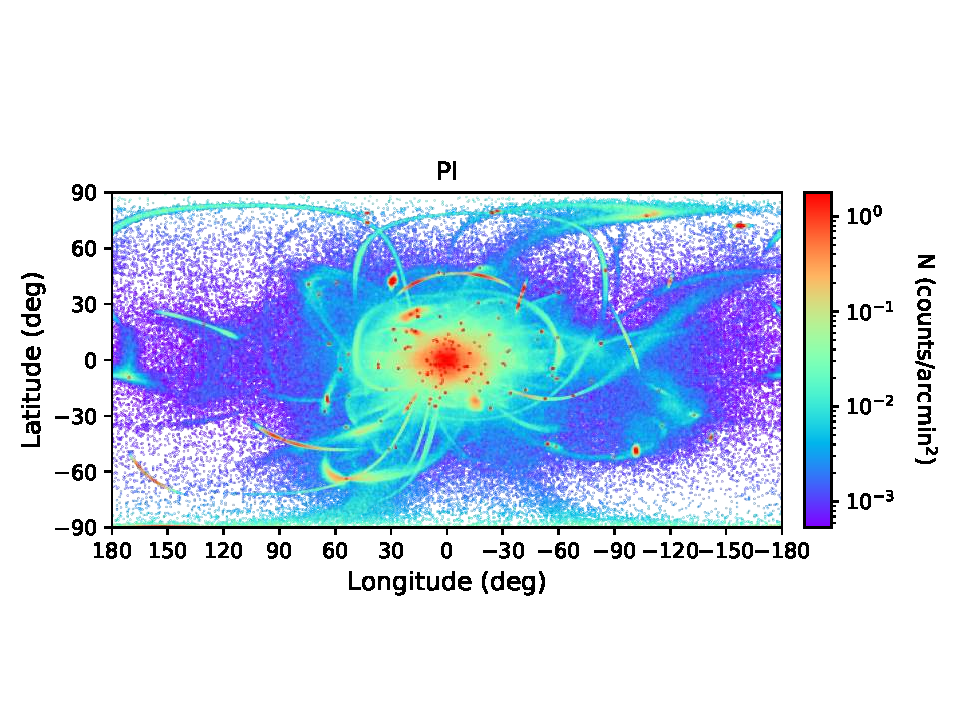
\includegraphics[clip=true, trim = 0mm 20mm 0mm 20mm, width=0.9\columnwidth]{images/PI_ensemble_LB_count_density.pdf}
            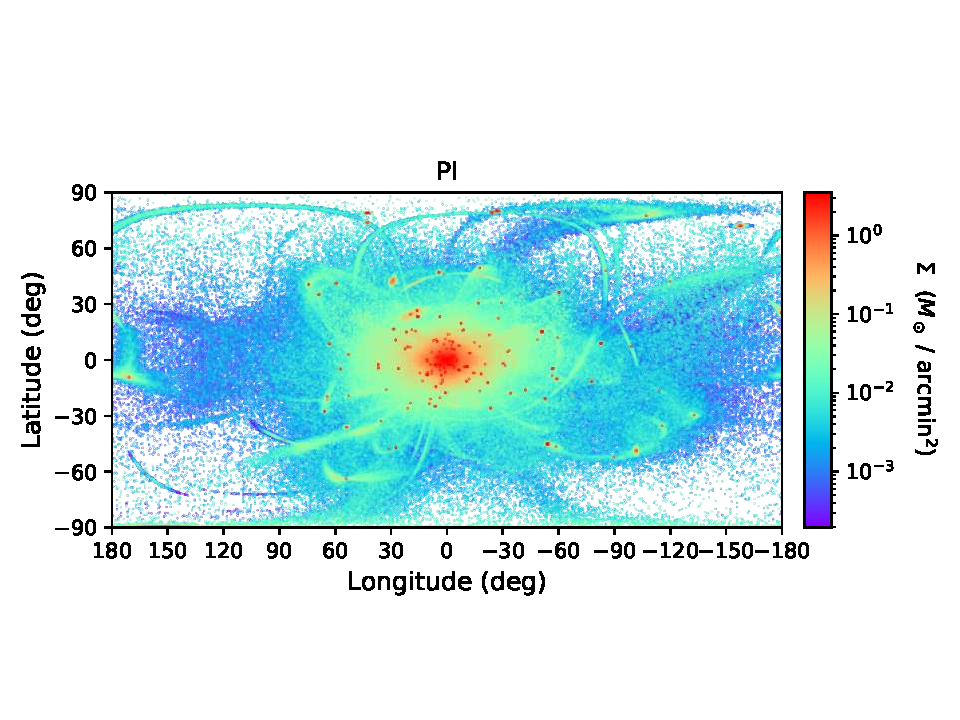
\includegraphics[clip=true, trim = 0mm 20mm 0mm 20mm, width=0.9\columnwidth]{images/PI_ensemble_LB_density_mass.pdf}
            
            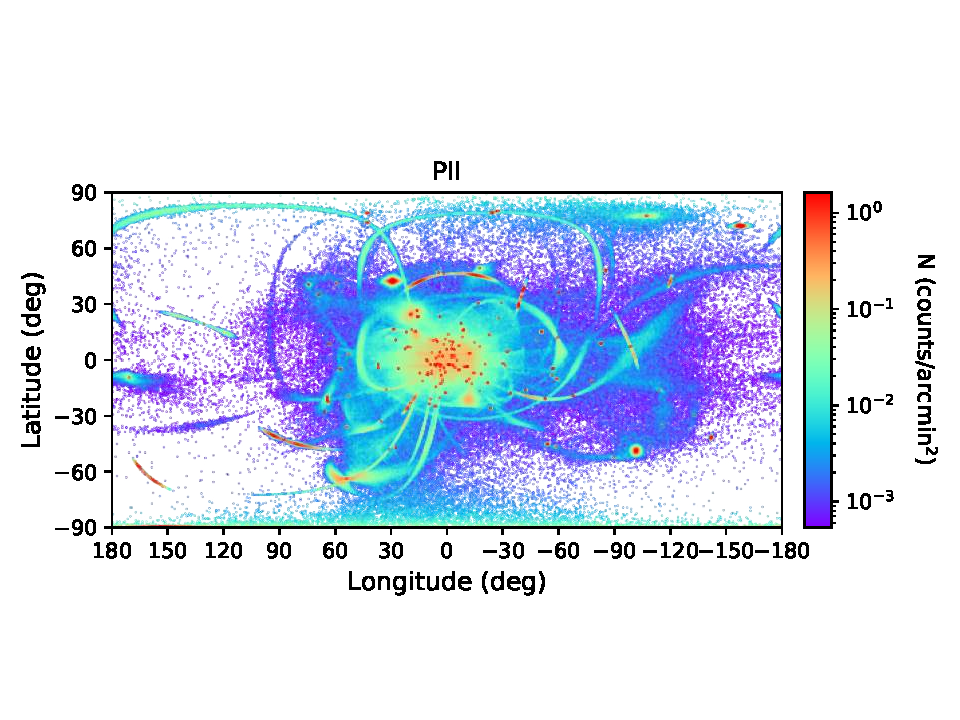
\includegraphics[clip=true, trim = 0mm 20mm 0mm 20mm, width=0.9\columnwidth]{images/PII_ensemble_LB_count_density.pdf}
            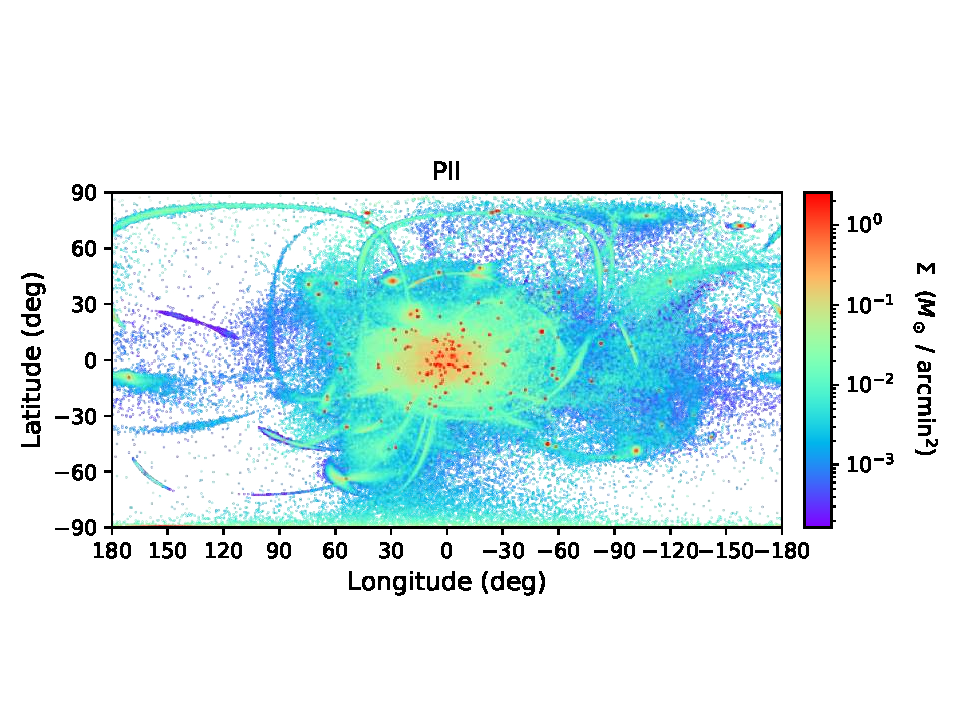
\includegraphics[clip=true, trim = 0mm 20mm 0mm 20mm, width=0.9\columnwidth]{images/PII_ensemble_LB_density_mass.pdf}

            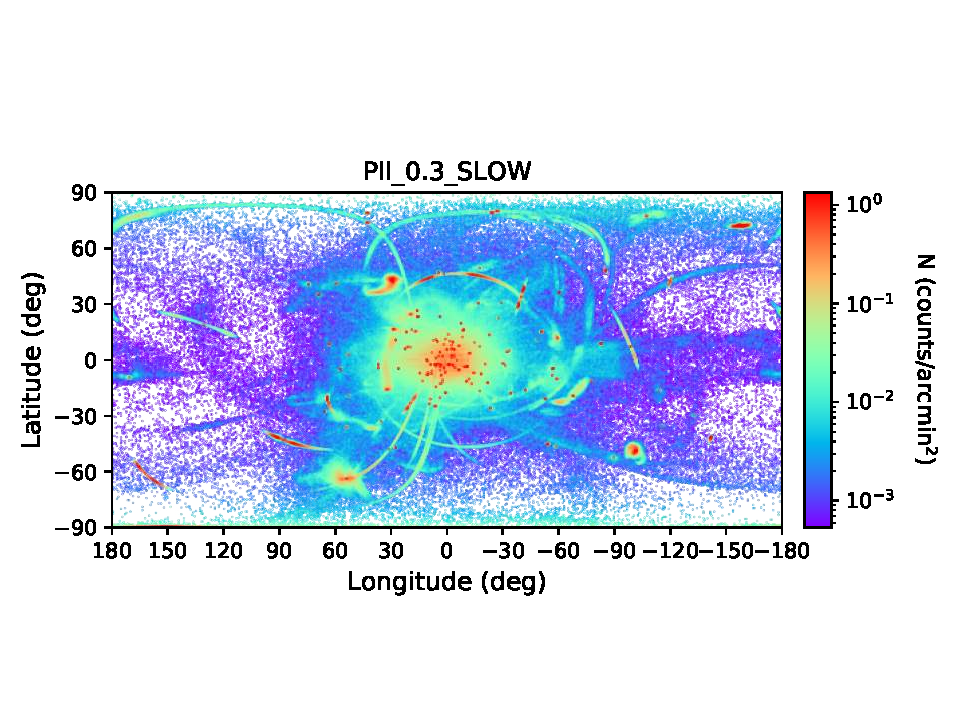
\includegraphics[clip=true, trim = 0mm 20mm 0mm 20mm, width=0.9\columnwidth]{images/PII_0.3_SLOW_ensemble_LB_count_density.pdf}
            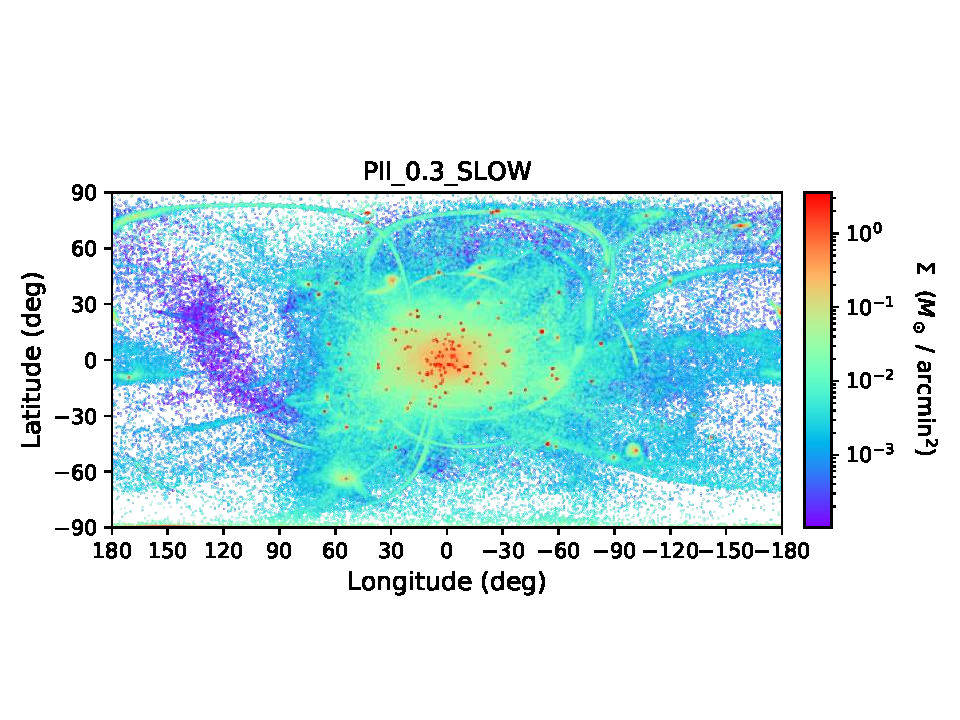
\includegraphics[clip=true, trim = 0mm 20mm 0mm 20mm, width=0.9\columnwidth]{images/PII_0.3_SLOW_ensemble_LB_density_mass.pdf}

            \caption{The stellar surface density of the \textit{ensemble} of extra-tidal features around the entire population of Galactic globular clusters at the current time, as predicted by our models. \textit{Left:} Surface number density. \textit{Right:} Surface mass density. Top row corresponds to model PI, the middle to model PII, and the bottom column to model PII-0.3-SLOW, as indicated. All densities are expressed in a logarithmic scale. The red point-like density maxima correspond to the current positions of the globular clusters. Values of higher density are overplotted. Thus in the case of mass density, diffuse tidal debris of more massive globular clusters covers the entire $(\ell,b)$ space and occults delicate tidal features, which are more visible when considering number density counts. In all panels, only the reference simulations are shown for clarity.} \label{galleryLB}
        \end{center}
    \end{figure*}
    \onecolumn

    \paragraph{A few basic premises:}
    Given the large number of simulations carried out and the wealth of information contained in them, it is not possible to exhaust all possible applications of this simulation database in this paper. We have therefore chosen to proceed as follows. 

    In Section~\ref{results1}, we present an overview of the distribution of all streams in  Galactic coordinates. This coordinate space will be the one used in the remainder of the entire article. This first section allows us to show qualitatively how the global distribution of streams varies, depending on the Galactic potential used.

    We  then move on (Section~\ref{streamvsD}) to present the global system of streams as a function of their distance from the Sun. In this section, we also show the kinematic properties of the streams, such as proper motions and line-of-sight velocities, that can be directly compared to Gaia data or other astrometric and spectroscopic surveys. This section also allows us to show the variety of morphologies that the stars which escaped from globular clusters can take. In Section~\ref{sec:morphologies}, we explore this issue in more detail, showing how these morphologies depend primarily on the orbital characteristics of the clusters and their distance from the Galactic center. For the most interesting cases, we compare the tidal structures predicted by our simulations with streams found in observational data. For this purpose, we make use of the \emph{galstreams} library of stellar streams in the Milky Way \citep{mateu22}, which constitutes a unique and public database summarizing angular positions, distances, proper motions, and line-of-sight velocity tracks for nearly a hundred Galactic stellar streams. Any stream that is not included in this library is not be compared to our simulations in the context of this paper.

    We note that the tidal features associated with each of the 159 simulated clusters are presented in Appendix~\ref{allstreams}. To avoid making this appendix too long, the  tidal features above are presented only in the case of the potential PII. However, all the data will be made available to the community at a dedicated site\footnote{\url{http://etidal-project.obspm.fr/}} where it is possible to  the way the characteristics of these streams change, for any cluster, in the three chosen potentials. 

    \subsection{A sky full of streams}\label{results1}

    Figure~\ref{galleryLB} shows the number and mass density distributions of the whole set of simulated globular clusters and their extra-tidal features in Galactic longitude and latitude for the three Galactic potentials.

    For all Galactic mass models adopted, a striking characteristic among the plots in Figs.~\ref{galleryLB} is the variety of features that our models predict, which are reminiscent of the tidal tails, stellar streams, and shells that are produced by interacting and merging galaxies in the process of mass assembly \citep[see, e.g., ][]{mancillas19}. Some clusters have very thin and elongated streams, which describe arcs that can extend up to $180^\circ$ in longitude, or tens of kpc in physical space. In some other cases, extra-tidal features appear shorter (a few up to ten degrees) and sometimes also thicker (about $10^\circ$ in the sky) than others. Finally, in some cases, clusters are surrounded by extended structures, such as halos, rather than coherent and thin streams. 

    This variety of properties depends on several factors: the distance of the stream to the Sun (due to projection; i.e., for a given physical thickness, the closer the stream is to the Sun, the more extended it appears in the $(\ell, b)$ plane), its orbital phase (towards the peri-center or the apo-center of the orbit), and the orbital properties of the parent globular cluster. We also see from these figures that stellar particles stripped from their parent clusters do not only redistribute in coherent structures, but in some cases, they can also contribute to a more diffuse density distribution. 

    Because of the large number of simulated clusters, we have chosen not to present the corresponding extra-tidal features one-by-one in the main part of this paper, but we have rather decided to describe these extra-tidal features with a global approach, by first adopting a criterion based on the distance of these features to the Sun (see Sect.~\ref{streamvsD}) and then discussing the types of distributions tidal debris can have and how these depend on the cluster orbital parameters (see Sect.~\ref{sec:morphologies}). All the extra-tidal structures generated by the 159 globular clusters simulated in this paper, and their corresponding uncertainties, are reported in Appendix~\ref{allstreams}. Among them, we include clusters with thin and elongated tails, such as IC~4499, NGC~3201, NGC~4590, NGC~5024, NGC~5053, Pal~5, to cite a few, as well as clusters such as AM~1, Pal~14, Pal~4, and Pal~15, whose extra-tidal material shows a halo-like configuration, and clusters such as NGC~1261, NGC~4147, NGC~6356, and UKS~1, whose stripped stars show a remarkable diffuse distribution in the field. 

    Finally, even when our models are not tailored to accurately reproduce the mass loss from globular clusters, since (as described in Sect.~\ref{initialconds}) we have adopted a test-particle approach with a time-constant globular cluster potential, it is however tempting to estimate, to a first order, the total mass associated with the tidally stripped population and compare it to the current mass. By calculating the mass lost in the field in the past 5~Gyr as the sum of the mass of all particles\footnote{\label{footnote:mass}To estimate the mass of particles in each cluster we have quantified the number of particles, $N_{bound}$, bound to the cluster at the end of the simulation and calculated the corresponding particle mass as $m_p=M_{GC}/N_{bound}$, where $M_{GC}$ is the current mass of a cluster given in Table~\ref{TableIC}.} that have escaped the cluster ($t_{\rm esc}> 0$), we find that the PI model sheds $2.1\times 10^{7} M_{\odot}$, which is 55\% of the GC population's current mass. The PII model shed is $2.7\times 10^{6} M_{\odot}$, which is 7\% of the current mass. Similarly, the PII-0.3-SLOW model lost $3.7\times 10^{6} M_{\odot}$, which is 10\% of the current mass and gives a half mass radius of 6.3~kpc.

    This mass roughly constitutes one-hundredth to one-tenth of the total stellar halo mass \citep{blandhawthorn16} and it is probably only a lower limit on the mass of escaped stars in the field, since a number of clusters initially in the Galaxy must have been destroyed over time (see introduction) and are thus no longer identifiabl as globular clusters today. It is also interesting to note that escaped stars are mostly redistributed in the inner Galaxy, with the half-mass radius of the PI model being 4.0~kpc and that of the PII and PII-0.3-SLOW models being 6.3~kpc. 

    The total mass lost from the clusters, as well as its spatial distribution, thus depends on the Galactic potential adopted: the variations between the PI model and both the PII and PII-0.3-SLOW models are of course caused by the PI's inclusion of the bulge, which leads to larger tidal forces in the center of the galaxy and subsequently drives larger mass loss. 

    Despite the differences in the modeling approach, it is interesting to compare our results to those of \citet{baumgardt2017global}. Briefly, our experiments differ in the following ways: they employ N-body simulations while we use our test-particle approach; they have an integration time of 12 Gyrs compared to our 5 Gyrs; lastly, their clusters have circular orbits in a Galactic potential modeled as an isothermal sphere as compared to the more realistic orbits and Galactic potentials considered in this work. Interestingly, the authors find that over 12 Gyrs their population of globular clusters lose two-thirds of their initial mass. This is roughly consistent with our application of the PI model, whose globular clusters shed 35\% of their initial mass in 5 Gyrs, which is roughly half the mass found by \citet{baumgardt2017global} in a period that is also about half as long. 

    \subsection{From the nearest to the furthest extra-tidal structures}\label{streamvsD}

    The analysis presented in this section along with the corresponding information are given in Figures~\ref{D0-10},~\ref{D10-20},~\ref{D20-30},~and~\ref{D30-300} are restricted to the PII model.

    \twocolumn
    \begin{figure*}[h!]
        \begin{center}
            \includegraphics[clip=true, trim = 0mm 15mm 0mm 20mm, width=0.9\columnwidth]{images/PII_ensemble_LB_D0-5_scatter.pdf}
            \includegraphics[clip=true, trim = 0mm 15mm 0mm 20mm, width=0.9\columnwidth]{images/PII_ensemble_LB_D5-10_scatter.pdf}

            \includegraphics[clip=true, trim = 0mm 20mm 0mm 20mm, width=0.9\columnwidth]{images/PII_ensemble_LB_D0-5_mass_est_new.pdf}
            \includegraphics[clip=true, trim = 0mm 20mm 0mm 20mm, width=0.9\columnwidth]{images/PII_ensemble_LB_D5-10_mass_est_new.pdf}

            \includegraphics[clip=true, trim = 0mm 20mm 0mm 20mm, width=0.9\columnwidth]{images/PII_ensemble_LB_D0-5_PML_new.pdf}
            \includegraphics[clip=true, trim = 0mm 20mm 0mm 20mm, width=0.9\columnwidth]{images/PII_ensemble_LB_D5-10_PML_new.pdf}

            \includegraphics[clip=true, trim = 0mm 20mm 0mm 20mm, width=0.9\columnwidth]{images/PII_ensemble_LB_D0-5_PMB_new.pdf}
            \includegraphics[clip=true, trim = 0mm 20mm 0mm 20mm, width=0.9\columnwidth]{images/PII_ensemble_LB_D5-10_PMB_new.pdf}

            \includegraphics[clip=true, trim = 0mm 20mm 0mm 20mm, width=0.9\columnwidth]{images/PII_ensemble_LB_D0-5_RV_new.pdf}
            \includegraphics[clip=true, trim = 0mm 20mm 0mm 20mm, width=0.9\columnwidth]{images/PII_ensemble_LB_D5-10_RV_new.pdf}
        \end{center}
    \caption{The extra-tidal features colored and weighted by various quantities within limited distance bins from the Sun projected in the $(\ell, b)$ plane. All outputs arrise from using the PII galactic potential model and only the reference simulation is shown in order to preserve clairty. \emph{Left column}: Extra-tidal features found at a distance of [0,5]~kpc from the Sun. \emph{Top row:} Scatter plot, with different colors indicating different progenitor clusters. \emph{Second row:} Mass density map in logarithmic scale. \emph{Third row:} Map color-coated by proper motions in longitudinal direction.    \emph{Fourth row:} Map color-coated by proper motions in latitudinal direction.  \emph{Bottom row:} Map color-coded by line-of-sight velocities. \emph{Right column}: Same as left column, but for the tidal features found at a distance of [5, 10]~kpc from the Sun. Note: the 10 colors used in the top panels are recycled between the 159 clusters, thus, all particles from the same cluster share one color, but a color is not unique to a cluster. }\label{D0-10}
    \end{figure*}
    \onecolumn

    \twocolumn
    \begin{figure*}[h!]
        \begin{center}
            \includegraphics[clip=true, trim = 0mm 15mm 0mm 20mm, width=0.9\columnwidth]{images/PII_ensemble_LB_D10-15_scatter.pdf}
            \includegraphics[clip=true, trim = 0mm 15mm 0mm 20mm, width=0.9\columnwidth]{images/PII_ensemble_LB_D15-20_scatter.pdf}

            \includegraphics[clip=true, trim = 0mm 20mm 0mm 20mm, width=0.9\columnwidth]{images/PII_ensemble_LB_D10-15_mass_est_new.pdf}
            \includegraphics[clip=true, trim = 0mm 20mm 0mm 20mm, width=0.9\columnwidth]{images/PII_ensemble_LB_D15-20_mass_est_new.pdf}

            \includegraphics[clip=true, trim = 0mm 20mm 0mm 20mm, width=0.9\columnwidth]{images/PII_ensemble_LB_D10-15_PML_new.pdf}
            \includegraphics[clip=true, trim = 0mm 20mm 0mm 20mm, width=0.9\columnwidth]{images/PII_ensemble_LB_D15-20_PML_new.pdf}

            \includegraphics[clip=true, trim = 0mm 20mm 0mm 20mm, width=0.9\columnwidth]{images/PII_ensemble_LB_D10-15_PMB_new.pdf}
            \includegraphics[clip=true, trim = 0mm 20mm 0mm 20mm, width=0.9\columnwidth]{images/PII_ensemble_LB_D15-20_PMB_new.pdf}

            \includegraphics[clip=true, trim = 0mm 20mm 0mm 20mm, width=0.9\columnwidth]{images/PII_ensemble_LB_D10-15_RV_new.pdf}
            \includegraphics[clip=true, trim = 0mm 20mm 0mm 20mm, width=0.9\columnwidth]{images/PII_ensemble_LB_D15-20_RV_new.pdf}
        \end{center}
        \caption{As for  Fig.~\ref{D0-10}, but for two father distance bins. Here, we are beyond the galactic nuclues and tidal debris are less diffuse in nature and more often stream-like. The \emph{left column} shows debris at distances between [10, 15]~kpc from the Sun while the \emph{right column} shows debris at distances between [15, 20]~kpc from the Sun.}\label{D10-20}
    \end{figure*}  
    \onecolumn  

    \twocolumn
    \begin{figure*}[h!]
        \begin{center}
            \includegraphics[clip=true, trim = 0mm 15mm 0mm 20mm, width=0.9\columnwidth]{images/PII_ensemble_LB_D20-25_scatter.pdf}
            \includegraphics[clip=true, trim = 0mm 15mm 0mm 20mm, width=0.9\columnwidth]{images/PII_ensemble_LB_D25-30_scatter.pdf}

            \includegraphics[clip=true, trim = 0mm 20mm 0mm 20mm, width=0.9\columnwidth]{images/PII_ensemble_LB_D20-25_mass_est_new.pdf}
            \includegraphics[clip=true, trim = 0mm 20mm 0mm 20mm, width=0.9\columnwidth]{images/PII_ensemble_LB_D25-30_mass_est_new.pdf}


            \includegraphics[clip=true, trim = 0mm 20mm 0mm 20mm, width=0.9\columnwidth]{images/PII_ensemble_LB_D20-25_PML_new.pdf}
            \includegraphics[clip=true, trim = 0mm 20mm 0mm 20mm, width=0.9\columnwidth]{images/PII_ensemble_LB_D25-30_PML_new.pdf}

            \includegraphics[clip=true, trim = 0mm 20mm 0mm 20mm, width=0.9\columnwidth]{images/PII_ensemble_LB_D20-25_PMB_new.pdf}
            \includegraphics[clip=true, trim = 0mm 20mm 0mm 20mm, width=0.9\columnwidth]{images/PII_ensemble_LB_D25-30_PMB_new.pdf}

            \includegraphics[clip=true, trim = 0mm 20mm 0mm 20mm, width=0.9\columnwidth]{images/PII_ensemble_LB_D20-25_RV_new.pdf}
            \includegraphics[clip=true, trim = 0mm 20mm 0mm 20mm, width=0.9\columnwidth]{images/PII_ensemble_LB_D25-30_RV_new.pdf}
        \end{center}
        \caption{As for  Fig.~\ref{D0-10}~\&~\ref{D10-20}, but for increased distances from the Sun. Here we notice that the tidal debris becomes more sparse as we move even father away from the galactic center. The \emph{left column} shows debris at distances between [20, 25]~kpc from the Sun while the \emph{right column} shows debris at distances between [25, 30]~kpc from the Sun.}\label{D20-30}
    \end{figure*}  
    \onecolumn  

    \twocolumn
    \begin{figure*}[h!]
        \begin{center}
            \includegraphics[clip=true, trim = 0mm 15mm 0mm 20mm, width=0.9\columnwidth]{images/PII_ensemble_LB_D30-35_scatter.pdf}
            \includegraphics[clip=true, trim = 0mm 15mm 0mm 20mm, width=0.9\columnwidth]{images/PII_ensemble_LB_D35-300_scatter.pdf}

            \includegraphics[clip=true, trim = 0mm 15mm 0mm 20mm, width=0.9\columnwidth]{images/PII_ensemble_LB_D30-35_mass_est_new.pdf}
            \includegraphics[clip=true, trim = 0mm 15mm 0mm 20mm, width=0.9\columnwidth]{images/PII_ensemble_LB_D35-300_mass_est_new.pdf}


            \includegraphics[clip=true, trim = 0mm 20mm 0mm 20mm, width=0.9\columnwidth]{images/PII_ensemble_LB_D30-35_PML_new.pdf}
            \includegraphics[clip=true, trim = 0mm 20mm 0mm 20mm, width=0.9\columnwidth]{images/PII_ensemble_LB_D35-300_PML_new.pdf}

            \includegraphics[clip=true, trim = 0mm 20mm 0mm 20mm, width=0.9\columnwidth]{images/PII_ensemble_LB_D30-35_PMB_new.pdf}
            \includegraphics[clip=true, trim = 0mm 20mm 0mm 20mm, width=0.9\columnwidth]{images/PII_ensemble_LB_D35-300_PMB_new.pdf}

            \includegraphics[clip=true, trim = 0mm 20mm 0mm 20mm, width=0.9\columnwidth]{images/PII_ensemble_LB_D30-35_RV_new.pdf}
            \includegraphics[clip=true, trim = 0mm 20mm 0mm 20mm, width=0.9\columnwidth]{images/PII_ensemble_LB_D35-300_RV_new.pdf}
        \end{center}
        \caption{As for  Fig.~\ref{D0-10}-\ref{D20-30}, but now we include debris from the most outer extent of  the galaxy. The \emph{left column} shows debris at distances between [30, 35]~kpc from the Sun while the \emph{right column} shows debris at distances between [35, 300]~kpc from the Sun.}\label{D30-300}
    \end{figure*}    
    \onecolumn
    In this section, we analyze structures located at different distances from the Sun. We identify structures as main or secondary on the basis of the fraction of stars they represent. If, for example, a cluster contributes more than 10\% of its stripped stars in a given distance range, we consider the associated structure to be significant and we define it as a main structure in this distance range. If, on the other hand, the fraction of stripped stars from a cluster is between 1\% and 10\%, we define the associated structure  as being "secondary." Structures that constitute less than 1\% of the cluster mass are considered insignificant in that range. The main and secondary structures for each distance bin are reported in Table~\ref{summarySTREAMS}, where they are named by their progenitor cluster. Below, we describe the structures encountered at different distances from the Sun, from the closest to the most distant. For the following discussions,  we refer to Figs.~\ref{D0-10} to \ref{D30-300}, where we report the different streams in a given distance range (top row in each figure), the corresponding mass density generated by all the structures found in that bin (second row), the longitudinal and latitudinal proper-motions map (third and fourth rows), and the line-of-sight velocities (bottom row).

    \paragraph{The [0--2]~kpc distance range: }
    Among the 159 simulated clusters, only  NGC~6121 is currently at a distance of less than 2~kpc from the Sun. In addition to stars stripped from this cluster within this distance-to-the-Sun range, we have identified very diffuse and low density extra-tidal stars associated with five other clusters, which are currently several kpc away from the Sun, as reported in Table~\ref{summarySTREAMS}. Of these, only UKS~1 and NGC~6121 have a significant fraction of their stripped mass in this distance range. All the others contribute with only a few percent. None of these clusters seem to show well-defined, stream-like features in the ($\ell,b$) plane. This extra-tidal material appears indeed quite uniformly redistributed, in a latitude range mostly inside $-30^\circ$ to $30^\circ$, and is mostly found at negative longitudes. Because in this interval range there is no remarkable extra-tidal structure found on the sky, we decided to plot this distance bin together with the [2--5]~kpc bin (see Fig.~\ref{D0-10}, left column).


    \paragraph{The [2--5]~kpc distance range: }
    As the distance from the Sun increases, many more tidal structures are intercepted. Eleven globular clusters are found at a distance between 2 and 5~kpc from the Sun; and together with structures emanating from these clusters, we also find extra-tidal material associated with other 48 clusters, 19 of which are significant (as listed in Table~\ref{summarySTREAMS}). Some extra-tidal structures are clearly identifiable, even when over-plotted with all the others: this is the case, for example, for the tidal material associated with the E~3 cluster, which appears as an extended thick stream (as shown in Fig.~\ref{D0-10}) at approximately $-100^{\circ}$ longitude. This is also the case for the complex tidal structure associated with BH~140, which resembles a ribbon in the sky, with a bifurcation at negative longitudes whose edges extend to about $-30^\circ$ and $30^\circ$ latitude. In addition to these, there are a series of circular halos concentric about the Galactic center, with abrupt drop-offs in density tracing the furthest extent of diffuse debris emanating from a variety of clusters. Overall, few streams are immediately recognizable in this range, although plenty of debris is present. This is expected given that this range samples a bite of the Sun-side of the Galactic disk and that this range has a relatively small volume. In this, as in the following distance ranges, the $v_{\ell os}$ maps show that the tidal material at negative Galactic longitudes has, on average, positive $v_{\ell os}$ while material at positive Galactic longitudes has, on average, negative $v_{\ell os}$, which is due to the solar reflex velocity. This is the same trend observed for the whole set of radial (i.e., line-of-sight) velocities in Gaia DR3; for instance, we refer to the bottom panel of Fig.~5 from \citet{katz22}, although less extreme velocities are reported in their plot since their dataset is dominated by disk stars, whereas our maps have a high proportional contribution of halo stars (additionally, they use median values in their bins, while we use an average). In order to quantify the net rotation of the system of streams, we calculated the mean angular momentum about the Galactic pole as $\braket{L_z} =\sum_i L_{z,i} m_{p,i} / \sum_i m_{p,i} $, where $m_{p,i}$ is the mass of each star particle indexed by $i$ (as discussed in footnote~\ref{footnote:mass}) and $L_{z,i}$ is the corresponding particle's angular momentum. The mean angular momentum is found to be $\braket{L_z}=-300$~kpc~km~s$^{-1}$, which shows a slight co-rotation of the system of streams with the disk though there is much dispersion about this value -- as shown in bottom right panel of Fig.~\ref{orbparam} in the Appendix.


    \paragraph{The [5--10]~kpc distance range: }
    The [5--10]~kpc distance range, which includes the Galactic center, contains much more material. A total of 79 clusters are found in this range, together with tidal structures associated with 131 different progenitors redistributed among main and secondary structures. Some tiny streams are visible in the density maps as well as in proper motions and line-of-sight velocity spaces (see Fig.~\ref{D0-10}, right column): the trailing portion of the tail of the globular cluster Pal~1, at $(\ell, b)\sim(140^\circ, 25^\circ)$; the most extreme portion of the trailing tail of NGC~3201 at $(\ell, b)\sim(150^\circ, -37^\circ)$; the waterfall-like shape of NGC~288, particularly evident at $b \lesssim -60^{\circ}$; the thin inverted U-shape of NGC~4590 at positive latitudes spanning a large longitude extent from $\ell \simeq -60^\circ$ to $100^\circ$; the portion of the E~3 tails the closest to the cluster at $(\ell, b)\sim(-75^{\circ},-15^{\circ})$, which continues from the more easily recognizable portion in the [0--5]~kpc bin.

    \paragraph{The [10--15]~kpc distance range: }
    In the [10--15]~kpc range, we find tidal structures associated with 134 progenitors, as listed in Table~\ref{summarySTREAMS} and reported in Fig.~\ref{D10-20} (left column), 27 of which are related to globular clusters that are also found in this distance bin. We note that at these distances from the Sun, the distribution of tidal features in directions towards the Galactic center, from $-30^{\circ}$ to $30^{\circ}$ longitude, appears less fuzzy than the one characterizing the [0--5] and [5--10]~kpc distance bins. Tidal features here are beyond the Galactic center, and are mostly associated with disk or halo clusters. 

    Among the thinnest structures, we find the stream associated with Pal~1, at $(\ell, b)\sim(120^\circ, 15^\circ),$ which is also visible in the distance bin [5--10]~kpc (see previous discussion), but which is even more elongated here. NGC~6101 shows the nearest portion of its long thin diagonal tidal tail that spans negative longitudes and ranges from $-15^{\circ}$ to $45^\circ$ latitude. Additionally, this stream is also unique against its counter parts in proper motion space. NGC~5053's nearest portion appears as a vertical tidal tail at $-80^{\circ}$ longitude. Similarly, NGC~5466 is shown vertically at $25^{\circ}$ longitude.

    Among the thickest structures, we can recognize general diffuse and bowtie-like shapes. There are also spoke-like structures departing radially from the Galactic center. For instance, we can associated the extra-tidal material with NGC~7078 at $(\ell, b)\sim(60^\circ,-28^{\circ}),$ as well as NGC~7089, which is nearly parallel to the previous structure, but at lower latitudes at $(\ell, b)\sim(50^\circ,-40^{\circ})$.

    \paragraph{The [15--20]~kpc distance range: }
    At larger distances ($[15--20]$~kpc range, see Fig.~\ref{D10-20}), some of the most striking features are associated with the clusters NGC~5024 and NGC~5053, whose long thin tails essentially overlap in this distance, with the latter covering the former, and appearing at high latitudes spanning a longitudinal range from $\ell \sim -90^{\circ}$ to $\ell \sim 45^{\circ}$. Again, the long thin stream of NGC~5466 appears in this range (as will be the case for the next) and is at high latitudes at roughly $85^{\circ}$ and positive longitudes. There is also the thicker extended structure of NGC~4147 whose diffuse structure emanates from about $(\ell, b)\sim(-100^{\circ},80^{\circ})$.

    In this distance bin, we find long tidal tails emanating from globular clusters associated  with the Sagittarius dwarf galaxy, which are particularly visible at negative longitudes: a long thin stream is associated  with Pal~12 at positive longitudes and latitudes $b \le-15^{\circ}$, as well as two overlapping structures at $0^\circ \lesssim \ell \lesssim 30^\circ$ longitude, namely, Ter~7 (and Ter~8 in the next distance bin). A word of caution is needed here: the mass loss from these clusters may be incorrect, since we do not include the presence of the Sagittarius dwarf galaxy itself. The potential well associated with this latter could change the tidal effects experienced by clusters associated with Sagittarius, especially in the case of NGC~6715, which sits at the center of this dwarf galaxy. The inclusion of the Sagittarius dwarf will be the subject of future investigations. Overall, in this distance bins, we find 11 clusters  and 61 streams, all listed in Table~\ref{summarySTREAMS}.

    \paragraph{The [20--25] and [25--30]~kpc distance ranges: }
    In the following distance bins (at [20--25]~kpc and [25--30]; see Fig.~\ref{D20-30}), globular clusters and extra-tidal structures become less numerous, although some are still visible, such as Pal~5 at $(\ell, b)\sim(0^{\circ},45^{\circ})$. In more detail, in the [20--25]~kpc bin we find tidal features associated  with 37 different progenitors, 8 of which are associated with globular clusters whose current positions are in the same distance bin; in the [25--30]~kpc bin, 7 clusters are found, together with tidal features associated with 30 other progenitor clusters which do not lie in this same distance range. In both bins, the streams emanating from globular clusters associated with the Sagittarius dwarf galaxy are still visible, as well as the most extreme portion of the tail associated with NGC~5466. 

    \paragraph{The [30--35] and [35--300]~kpc distance ranges: }
    Finally, in the last distance bins (see Fig.~\ref{D30-300}), thin streams become rare. Some small streams are visible: Pyxis at $(\ell, b)\sim(-100^{\circ},0^{\circ})$; NGC~2419 at $(\ell, b)\sim(-180^{\circ},30^{\circ})$; Pal~4 at $(\ell, b)\sim(-160^{\circ},75^{\circ})$; Pal~3 at $(\ell, b)\sim(-120^{\circ},45^{\circ})$. Many more have a diffuse and halo-like structure. For instance, the blob associated with Pal~15, centered at $(\ell, b)\sim (15^\circ, 20^\circ$); AM~1 at $(\ell, b)\sim(-100^{\circ},-55^{\circ})$; Eridanus at $(\ell, b)\sim(-140^{\circ},-45^{\circ})$; Pal~14 at $(\ell, b)\sim(30^{\circ},45^{\circ})$; Laevens~3 at $(\ell, b)\sim(65^\circ,-20^\circ)$, which is completely enveloped by NGC~7006. In total, in these two distance bins, we find 4 and 12 clusters, respectively, along with their associated streams, together with extra-tidal material associated with 14 and 19 progenitors in total. 


    \begin{table*}
        \tiny
        \centering                                      % used for centering table
        \caption{List of tidal structures found in different intervals of distance to the Sun. The tidal structures are named by their progenitor clusters. If the parent cluster is also in the distance range under consideration, the name of the tidal structure is shown in bold. Second column reports the main structures found in a given distance bin. The third column list secondary structures. The numbers in parenthesis in the second column  and third column (numbers with normal font) correspond to the total number of main and secondary structures found in a given distance range. The number of clusters in each distance bin is also reported in the second column (bold numbers in parenthesis). }\label{summarySTREAMS}
        \begin{tabularx}{\textwidth}{l X X }          % centered columns (4 columns)
        \hline
        Distance (kpc) &   Main tidal structures & Secondary tidal structures\\ 
        %(kpc) &  \\ 
        \hline   \\
        \tiny
        \vspace{0.1cm}
        [0-2] & (\textbf{1},2) \textbf{NGC6121}, UKS1 & (4) BH140, Djor1, NGC6333, NGC6356\\ 
        \vspace{0.1cm}

        [2-5] & (\textbf{11},30) \textbf{NGC6397}, \textbf{NGC6544}, \textbf{NGC3201}, \textbf{BH140}, \textbf{NGC104}, \textbf{NGC6838}, \textbf{NGC6366}, \textbf{NGC6752}, \textbf{IC1276}, \textbf{NGC6656}, \textbf{2MASS-GC01}, NGC6284, NGC6356, NGC6287, VVV-CL001, NGC6254, NGC5927, E3, NGC6121, VVV-CL001, Djor1, UKS1, Ter10, 2MASS-GC02, Pal10, NGC5139, NGC6333, NGC6441, NGC6541, NGC288 & (29) FSR1716, FSR1758, NGC1851, NGC1904, NGC2298, NGC2808, NGC362, NGC4372, NGC4833, NGC5897, NGC5986, NGC6205, NGC6218, NGC6235, NGC6273, NGC6316, NGC6352, NGC6388, NGC6496, NGC6681, NGC6749, NGC6760, NGC6809, NGC6864, NGC7078, Pal2, Pal8, Ter12, Ton2\\ 
        \vspace{0.1cm}

        [5-10] & (\textbf{79},124) \textbf{VVV-CL001}, \textbf{NGC7099}, \textbf{NGC6362}, \textbf{Ton2}, \textbf{Djor1}, \textbf{VVV-CL001}, \textbf{NGC6496}, \textbf{Djor2}, \textbf{NGC6535}, \textbf{NGC6528}, \textbf{NGC6539}, \textbf{NGC6540}, \textbf{NGC6553}, \textbf{2MASS-GC02}, \textbf{Ter12}, \textbf{BH261}, \textbf{Ter9}, \textbf{NGC6712}, \textbf{NGC6717}, \textbf{NGC6723}, \textbf{NGC6749}, \textbf{NGC6760}, \textbf{Pal10}, \textbf{HP1}, \textbf{Ter4}, \textbf{Ter2}, \textbf{Ter3}, \textbf{NGC2298}, \textbf{E3}, \textbf{NGC4372}, \textbf{NGC4833}, \textbf{NGC5904}, \textbf{NGC5927}, \textbf{FSR1716}, \textbf{Lynga7}, \textbf{NGC6144}, \textbf{NGC6171}, \textbf{NGC6352}, \textbf{ESO452-SC11}, \textbf{NGC6218}, \textbf{FSR1735}, \textbf{NGC6254}, \textbf{NGC6256}, \textbf{NGC6287}, \textbf{NGC6293}, \textbf{NGC6304}, \textbf{NGC6355}, \textbf{NGC6809}, \textbf{NGC6637}, \textbf{NGC6402}, \textbf{NGC6325}, \textbf{NGC6341}, \textbf{NGC6342}, \textbf{NGC6380}, \textbf{NGC6401}, \textbf{NGC6440}, \textbf{NGC6517}, \textbf{NGC6522}, \textbf{NGC6541}, \textbf{NGC6558}, \textbf{NGC6624}, \textbf{NGC6626}, \textbf{NGC6638}, \textbf{NGC6642}, \textbf{NGC6652}, \textbf{NGC6681}, \textbf{Pal6}, \textbf{Ter1}, \textbf{Ter5}, \textbf{Ter6}, \textbf{NGC6333}, \textbf{NGC288}, \textbf{NGC362}, \textbf{NGC6273}, \textbf{NGC6266}, \textbf{NGC6205}, \textbf{NGC5139}, \textbf{Liller1}, \textbf{NGC5946}, NGC5897, NGC1904, NGC6752, NGC6656, NGC6121, NGC1851, NGC6864, NGC7078, NGC7089, NGC6316, NGC5272, NGC6779, NGC2808, NGC4590, Rup106, NGC104, NGC4147, NGC3201, Pal11, Pal1, NGC1261, BH140, NGC6235, Ter10, NGC6569, UKS1, NGC6453, NGC6139, NGC6426, NGC6397, NGC6093, NGC6388, FSR1758, IC1276, NGC6838, NGC6366, NGC5986, NGC6441, NGC6356, NGC6584, NGC5286, NGC6544, NGC6284, Pal8, NGC6981 & (7) 2MASS-GC01, IC1257, NGC5634, NGC5694, NGC6229, NGC7006, Pal2\\ 
        \vspace{0.1cm}

        [10-15] & (\textbf{27},115) \textbf{NGC6453}, \textbf{NGC5272}, \textbf{NGC6584}, \textbf{Pal8}, \textbf{NGC6316}, \textbf{NGC5897}, \textbf{NGC6284}, \textbf{NGC6139}, \textbf{NGC6093}, \textbf{NGC5986}, \textbf{NGC5286}, \textbf{NGC6235}, \textbf{NGC2808}, \textbf{NGC1904}, \textbf{NGC1851}, \textbf{NGC6101}, \textbf{NGC6779}, \textbf{NGC6388}, \textbf{Pal11}, \textbf{Pal1}, \textbf{Ter10}, \textbf{NGC4590}, \textbf{NGC7089}, \textbf{NGC6569}, \textbf{NGC7078}, \textbf{FSR1758}, \textbf{NGC6441}, NGC6304, NGC6254, FSR1735, NGC6426, NGC6397, NGC6362, Ton2, NGC6256, NGC6366, NGC6287, NGC6352, NGC6355, NGC6356, NGC6218, NGC6293, VVV-CL001, NGC6171, NGC5024, NGC1261, NGC2298, E3, NGC3201, NGC4147, NGC4372, Rup106, BH140, NGC4833, NGC5053, Ter3, NGC5466, NGC5634, IC4499, NGC5904, NGC5927, FSR1716, UKS1, NGC6121, NGC6144, Lynga7, NGC6553, VVV-CL001, NGC6496, NGC5946, NGC6205, NGC6266, NGC6273, NGC6333, NGC6341, NGC6342, NGC6401, NGC6402, NGC6517, NGC6541, NGC6544, NGC6558, NGC6626, NGC6652, NGC6656, NGC6681, NGC6864, Pal6, Ter1, Ter5, NGC5139, NGC362, NGC104, Ter12, Djor2, NGC6535, NGC6528, NGC6539, NGC6540, 2MASS-GC01, Ter9, 2MASS-GC02, IC1276, BH261, NGC7099, NGC6712, NGC6723, NGC6749, NGC6752, NGC6760, NGC6809, NGC6838, NGC6934, NGC6981, NGC288 & (18) Djor1, ESO280-SC06, ESO452-SC11, HP1, IC1257, NGC5694, NGC5824, NGC6229, NGC6325, NGC6380, NGC6638, NGC6642, NGC6717, NGC7006, NGC7492, Pal10, Pal2, Ter6\\ 
        \vspace{0.1cm}

        [15-20] & (\textbf{11},46) \textbf{NGC6356}, \textbf{NGC5466}, \textbf{NGC1261}, \textbf{UKS1}, \textbf{NGC4147}, \textbf{IC4499}, \textbf{NGC5024}, \textbf{NGC5053}, \textbf{Pal12}, \textbf{NGC6981}, \textbf{NGC6934}, NGC6101, NGC5904, Pal5, NGC5824, NGC5634, NGC7089, FSR1758, NGC4833, BH140, NGC4590, Rup106, NGC3201, Pal2, NGC5272, Djor1, NGC6426, NGC7078, NGC6864, NGC6715, NGC6656, NGC6341, NGC6333, NGC5286, NGC362, NGC2808, NGC1851, NGC104, NGC7492, Pal10, Ter7, NGC6779, NGC6584, IC1276, ESO280-SC06, NGC288 & (15) 2MASS-GC02, IC1257, NGC1904, NGC2298, NGC4372, NGC5139, NGC5694, NGC6121, NGC6205, NGC6229, NGC6838, NGC7006, NGC7099, Pal13, Ter8\\ 
        \vspace{0.1cm}

        [20-25] & (\textbf{8},29) \textbf{Pal5}, \textbf{NGC7492}, \textbf{Pal13}, \textbf{Rup106}, \textbf{NGC6864}, \textbf{NGC6426}, \textbf{ESO280-SC06}, \textbf{Ter7}, NGC5466, IC4499, NGC5634, NGC7089, NGC5824, NGC5024, NGC4590, NGC4147, NGC3201, NGC5272, IC1257, NGC5904, NGC6101, NGC6584, Arp2, Ter8, NGC6934, NGC6981, Pal12, NGC6229, Pal2 & (9) Djor1, FSR1758, NGC1261, NGC1851, NGC1904, NGC2298, NGC2808, NGC5694, NGC7006\\ 
        \vspace{0.1cm}

        [25-30] & (\textbf{7},20) \textbf{NGC6715}, \textbf{Pal2}, \textbf{AM4}, \textbf{NGC5634}, \textbf{Ter8}, \textbf{Arp2}, \textbf{IC1257}, NGC5824, Rup106, NGC5694, IC4499, NGC6101, NGC5904, NGC6229, Ter7, NGC6934, NGC6981, Pal13, NGC7492, Whiting1 & (10) NGC1851, NGC1904, NGC3201, NGC4147, NGC4590, NGC5466, NGC7006, NGC7089, Pal15, Pyxis\\ 
        \vspace{0.1cm}

        [30-35] & (\textbf{4},11) \textbf{NGC6229}, \textbf{NGC5824}, \textbf{NGC5694}, \textbf{Whiting1}, NGC7006, Ter8, Arp2, Ter7, Rup106, Pyxis, Pal2 & (3) NGC6101, NGC6934, Pal15\\ 
        \vspace{0.1cm}

        [35-300] & (\textbf{12},15) \textbf{Laevens3}, \textbf{NGC7006}, \textbf{SagittariusII}, \textbf{Pal15}, \textbf{Pal14}, \textbf{Crater}, \textbf{Pal4}, \textbf{Pal3}, \textbf{Pyxis}, \textbf{NGC2419}, \textbf{Eridanus}, \textbf{AM1}, NGC6715, NGC5824, NGC5694 & (4) Arp2, NGC6934, Pal2, Ter8
        \end{tabularx}
        \normalsize
    \end{table*}


    \subsection{Disks of inner and outer halo clusters: A variety of morphologies and shapes for extra-tidal structures}\label{sec:morphologies}
        The analysis presented in the previous section allows us to appreciate the variety of morphologies found for extra tidal structures, from padlocks to ``Easter eggs,'' disks, ribbons, and canonical streams. Moreover, some structures are limited in latitude and longitude, while some others fill nearly the entire sky. 

        To more easily capture the similarity and differences in the morphology of the extra-tidal features surrounding Galactic globular clusters, we can group the latter on the basis of their orbital parameters\footnote{We caution the reader that the classification of disk, inner and outer clusters made in this Section is based on the orbital parameters of the clusters, as found when their orbits are integrated in model PII. This classification may slightly change if model PI or model PII-0.3-SLOW were adopted.}(see Appendix~\ref{class} for more details), as follows: \emph{Disk clusters}: A cluster is classified as a disk cluster if arctan($z_{max}/R_{max}$) $\le 10^\circ$, where $z_{max}$ and $R_{max}$ are, respectively, the maximum height above or below the Galactic plane reached by its orbit in the last 5~Gyr and its maximum in-plane distance from the Galactic center. \emph{Inner clusters}: All clusters with $r_{max} \le R_{\odot}$ that are not classified as disk clusters enter this group. Contrary to $R_{max}$, which is the maximum in-plane distance that a cluster reaches from the Galactic center, $r_{max}$ is the maximum 3D distance, that is, $r_{max} = \textrm{max}(\sqrt{R^2+z^2}),$ with the maximum calculated over the whole cluster orbit. \emph{Outer clusters}: All clusters with $r_{max} > R_{\odot}$ that are not classified as disk clusters are included in this group. 

        By using the orbital radius of the Sun as the criterion for inner and outer clusters, debris from outer clusters can span the whole sky while inner clusters must be restricted in longitude and latitude. With these definitions, 21 clusters are disk clusters, 71 are inner clusters, and 67 are outer clusters (see  Table~\ref{classification} in Appendix~\ref{class}). We emphasize that this classification does not aim to suggest any specific origin for these systems \citep[e.g., whether they are in-situ or accreted, see][]{massari19}, but it is uniquely based on their current orbital characteristics and helps in capturing some of the properties in the extension (projected in to the sky) and shape of their extra-tidal material, as we discuss in the following.

        \subsubsection{Extra-tidal features originating from disk clusters: ribbons in the Galactic plane}

            Disk clusters are defined on the basis of the flatness of their orbits (i.e., on their $z_{max}/R_{max}$ ratio). As a result, they typically are restricted to low latitudes, though the exact distribution depends on the relationship of their orbit to the solar radius. To specify, clusters whose $R_{max}$ are interior to the Solar radius generate tidal debris in a limited range in longitude and latitude. For instance, the material associated with clusters as Ter~1, Ter~5, Ter~6, and Ter~9 has a disk-like shape and is completely confined to $|\ell| <30^{\circ}$ and $|b|<10^{\circ}$. If $R_{max}$ is greater than the solar radius, material can cover the full longitude space and most of the material will still appear at low latitudes. This is the case, for example, of BH~140, whose escaped stars diffusely occupy all longitudes and most of them are found at $|b| \le 30^\circ$, while for Pal~2 and Pal~10, their extra-tidal stars have a very limited latitudinal extension and appear as ribbons in the sky. In the following, we discuss some of the structures associated with NGC~6121, Pal~2, and Pal~10. We refer to Appendix~\ref{allstreams} for the tidal structures generated by the whole set of disk clusters.  

            \twocolumn
            \begin{figure}
                \begin{center}
                    \includegraphics[clip=true, trim = 0mm 2mm 0mm 0mm, width=0.9\columnwidth]{images/PII_individual_NGC6121_NGC6121orbitRZXY.pdf}

                    \includegraphics[clip=true, trim = 0mm 20mm 0mm 10mm, width=0.9\columnwidth]{images/PII_individual_NGC6121_NGC6121orbit.pdf}

                    \includegraphics[clip=true, trim = 0mm 20mm 0mm 10mm, width=0.9\columnwidth]{images/PII_individual_NGC6121_NGC6121_LB_D.pdf}

                    \includegraphics[clip=true, trim = 0mm 20mm 0mm 10mm, width=0.9\columnwidth]{images/PII_individual_NGC6121_NGC6121_LB_tesc.pdf}
                \end{center}
                \caption{ \emph{Top-left panel:} Projection of the orbit of NGC~6121 in the meridional $\rm R-z$ plane. Colors trace time, from 5~Gyr ago (negative values) to 5~Gyr forward in time (positive values). \emph{Top-right panel:} Projection of the orbit of NGC~6121 in the Galactic $x-y$ plane.  \emph{Second row:} Projection of the NGC~6121 orbit for the past and future 5~Gyr, in the longitude-latitude plane.   \emph{Third row:} Projection in the longitude-latitude plane of the extra-tidal material lost by NGC~6121. Colors indicate the average distance of the stripped material from the Sun.  \emph{Bottom panel:} Projection in the longitude-latitude plane of the extra-tidal material lost by NGC~6121. Colors indicate the average time at which stellar particles become gravitationally unbound to the cluster, from 5~Gyr ago (negative time) to the current time ($\textrm{escape time} = 0$). In the bottom and middle panels, only the reference simulation without errors is shown for clarity. In all plots, the current position of the cluster is given by the white circle with a black outline. The yellow star, when present, indicates the position of the Sun. }\label{ngc6121_stream}
            \end{figure}
            \onecolumn


\chapter{Gapology}
\section{Published results}

  \begin{figure*}
    \centering
    \includegraphics[width=\linewidth]{images/stream_on_sky_Pal5_monte-carlo-009_pouliasis2017pii-GCNBody_pouliasis2017pii.png}
    \caption{Simulated Palomar~5 stream created by modeling the host cluster as a Plummer sphere disrupting within an axis-symmetric Galactic potential plus the gravitational effect of 164 other Galactic globular clusters. The top panel shows the distribution of star particles that escaped the cluster due to tidal forces. The bottom panel shows the 1D density profile marginalized over longitude. The gray fill shows a reference simulation that uses the same conditions to produce the stream but does not include the other globular clusters. The large central peak in density is composed of particles still bound to Palomar~5. $\ell_0,b_0$ are located Palomar~5's cluster's center of mass. Two large gaps are present due to the passage of two globular clusters. $N_p$ indicates the number of particles in a bin, while $N$ is the total number of particles, which is 100,000.}
    \label{fig:stream_on_sky}
    \end{figure*}

\section{Methods}
    The most accurate model of the Palomar~5 stream would involve full modeling of the internal dynamics of the cluster, which would mean computing $N$-body interactions with a $\mathcal{O}(N^2)$ computation time, stellar evolution, supernovae, an initial mass distribution, treatment of binary star systems, etc. \citep[for such an example, see][]{2021NatAs...5..957G, 2016MNRAS.458.1450W}. Instead, we opt for solving the restricted-three-body problem, also known as the particle-test method, as we did for \citet{2023A&A...673A..44F}, which we describe here for completeness. As demonstrated by \citet{2012A&A...546L...7M}, although the restricted three-body problem neglects the internal evolution of the cluster, it still reproduces very similar stream properties since the model captures key extracluster physics, such as disk shocking and epicyclic stripping.\\

    Below, we first present the approach used to include the Galactic globular cluster system in our modeling (Sect.~\ref{numerical_meth}), highlighting the similarities and differences with respect to what we did in \citet{2023A&A...673A..44F}; we then summarize the method used to model the mass loss from the cluster (Sect.~\ref{sec:mass_loss}) and finally discuss the quality of the numerical integration (Sect.~\ref{num_quality}). 

    \subsection{Numerical methodology}\label{numerical_meth}
        We begin by extracting positions in the sky, proper motions, line-of-sight velocities, and distances, as well as masses and half-mass radii, of 165 globular clusters from the Galactic globular cluster catalog by \cite{2021MNRAS.505.5957B}.\footnote{The Baumgardt catalog has been assembled across a series of works, see: \cite{2020PASA...37...46B,2019MNRAS.482.5138B,2018MNRAS.478.1520B}. The catalog can be found on the World Wide Web at \href{https://people.smp.uq.edu.au/HolgerBaumgardt/globular/}{https://people.smp.uq.edu.au/HolgerBaumgardt/globular/}.} We then convert the initial conditions from sky coordinates into a Galactocentric reference frame, by adopting a velocity for the local standard of rest of $v_{\text{LSR}} = 240$~km~s$^{-1}$ and a peculiar velocity of the Sun equal to $(U_\odot, V_\odot, W_\odot)=(11.1, 12.24, 7.25)$~km~s$^{-1}$, as reported by \citet{2012MNRAS.427..274S}.  We set the Sun's position to $(x_\odot,y_\odot,z_\odot) = (-8.34,0,0.027)$~kpc. We took the vertical position above the disk from \citet{2001ApJ...553..184C} and the distance of the Sun to the Galactic center from \citet{2014ApJ...783..130R}. These transformations were performed using \texttt{astropy} \citep{2013A&A...558A..33A}.

        For the Galactic potential, we employed the second model from \citet{2017A&A...598A..66P}, a superposition of a thin disk, thick disk, and dark matter halo, with masses and scale lengths provided in Table~1 of \citet{2023A&A...673A..44F}. This model is time-independent throughout our simulations. This model satisfies a series of observational constraints such as local solar, stellar density, the Galactic rotation curve, similarly to other Galactic models such as \texttt{MWpotential2014} from \citet{2015ApJS..216...29B} and \texttt{McMillian2017} from \citet{2017MNRAS.465...76M}. However, we use only one Galactic potential to balance data volume and computation time, which should suffice. \citet{2021MNRAS.505.5978V} found that only a few outer globular clusters are strongly affected by different potential models. Generally, kinematic uncertainties are the dominant factor in differences between orbital solutions per cluster. Similarly, \citet{2024MNRAS.528.5189G} generated a globular cluster mass-loss catalog using seven different potential models and found that their debris distributions were rather model-independent, similar to those of \citet{2023A&A...673A..44F}. While the clusters' exact positions in time may depend on the model, we assert that interaction rates and stream formation are largely independent of the choice of the Galactic potential model.
    
        Lastly, we select an integration time of 5~Gyr as a compromise between maximizing interaction statistics and modeling the Galaxy as a time-independent, constant mass distribution. \citet{2023A&A...673A.152I} analyzed the orbits of the Galactic cluster population using the same initial conditions as in this work within five live Milky Way-like potentials from IllustrisTNG \citep{2018MNRAS.473.4077P}. They found that in all sampled potentials, orbital changes remain minimal over 5~Gyr, becoming significant only at earlier look-back times when the host galaxy had significantly less mass or was undergoing a merger event.


        \subsubsection{ \texttt{Full} simulations}
            There is a primary methodological departure from \citet{2023A&A...673A..44F}.  In that work, globular clusters evolved under the gravitational effect of the Galaxy alone. In contrast, now we also consider the effect of all other Galactic globular clusters by taking into account the direct $N$-body interactions between them. First, all clusters are represented by Plummer spheres, each with its own mass and half-mass radius as reported in the Baumgardt catalog \citep{2021MNRAS.505.5957B}. For the remainder of this paper, the \texttt{full} simulations consider the gravitational forces from the globular cluster interactions. \\
            For these simulations, we proceeded in two steps:
            \begin{enumerate}
                \item First, starting from the Galactocentric positions and velocities of all 165 Galactic globular clusters, we integrate their orbits back in time for 5~Gyr under the influence of the Galaxy itself and their mutual influence. In the backward integration, the system of equations of motion for the globular clusters is thus: 
                \begin{equation}
                    \ddot{\vec{r}}_i = -\nabla \Phi + \left.\sum_{j\neq i}^{N_{GC}} \frac{Gm_j}{\left(|\vec{r}_j - \vec{r}_i|^2 + b_j^2\right)^{3/2}}\right. \left(\vec{r}_j - \vec{r}_i\right),
                \end{equation}\label{eq:GCNBody} 
                \noindent where $\vec{r}$ indicates the Galactocentric position vector, the index $i$ indicates the globular cluster of interest; the index $j$ indicates the other globular clusters that are summed over. $N_{GC}$ is the total number of globular clusters, which in this study is 165, $m_j$ is the mass of the j-th cluster in the sample, $b_j$ is its Plummer scale radius, and $\vec{r_j}$ is its Galactocentric position. $\Phi$ represents the same Galactic smooth potential that we discussed previously \citep[][Model~II, in the present case]{2017A&A...598A..66P}. Note that the masses and sizes of the globular clusters are kept constant in these simulations and are not allowed to vary with time, which means that we do not consider their internal evolution. In sec.~\ref{sec:discussion}, we discuss the implications of the modeling limitations.
                \item Once we found the positions and velocities of the entire globular cluster, we sampled Palomar~5 with 100,000 particles from a Plummer distribution, taking the mass and half-mass radius from the Baumgardt catalog: $1.3\times10^{4}~\textrm{M}_\odot$ and $27.6~\textrm{pc}$. We then integrated the evolution of these particles forward in time to the present day, taking into account that each particle feels the gravitational potential of the Galaxy, its host cluster, and that of all the other clusters in the Galaxy. Note that we do not account for self-gravity among particles. The particles experience the gravitational field yet do not contribute to it, a common assumption in galactic dynamics, as the mass of an individual star is negligible compared to the mass of the larger dynamical system. The equation of motion of a generic particle among the 100,000 that populate Palomar~5 is thus: 
                \begin{equation}
                    \ddot{\vec{r}}_p = -\nabla \Phi + \left.\sum_{j}^{N_{GC}} \frac{Gm_j}{\left(|\vec{r}_j(t) - \vec{r}_p|^2 + b_j^2\right)^{3/2}}\right. \left(\vec{r}_j(t)- \vec{r}_p\right),
                \end{equation} \label{eq:equation_of_motion_particle} where the index $p$ represents one of the 100,000 particles of interest, $\vec{r_p}$ being its position, and $j$ indexes over the globular clusters as in Eq.~\ref{eq:GCNBody}. We note that in Eq.~\ref{eq:equation_of_motion_particle}, the positions of the globular clusters are time-dependent since they are being loaded during this step and not computed, unlike Eq.~\ref{eq:GCNBody}. 
            \end{enumerate}

            The procedure described so far has been repeated 50 times, generating a new set of initial conditions each time, given the uncertainties on proper motions, line-of-sight velocities, distances to the Sun, and masses of all clusters, as reported in the Baumgardt catalog. We handle these uncertainties through a Monte-Carlo approach by sampling them with a Gaussian distribution and considering the covariance term between the proper motions. We use the most probable values for the initial conditions in the first simulation. We sample the uncertainties for all globular clusters. Additionally, for each resampling of Palomar~5's mass, we also resample the distribution of the 100,000 star particles. 

            During the integration, we save intermediate snapshots to facilitate the analysis of stellar streams and the effects of cluster impacts. Specifically, for each realization of the Palomar~5 stream, we saved $5000$ in snapshots, equivalent to a temporal resolution of 1 million years. We provide the parameters that specify our data volume in Table~\ref{tab:data_volume}. Using single precision floating point numbers, the size of our simulations is approximately:
            \begin{equation} \label{eq:data_volume_estimate}
                N_p \times N_{\textrm{ts}}\times N_{\textrm{phase}}\times N_{\textrm{sampling}} \times 4~\textrm{bytes}\approx 600~\textrm{Gb}.
            \end{equation}

            \begin{center}
                \begin{table}[h]
                    \centering
                    \caption{Parameters determining the data volume.}
                    \label{tab:data_volume}
                    \begin{tabular}{|c|c|c|c|}
                        \hline
                        $N_p$ & $N_{\textrm{ts}}$ & $N_{\textrm{phase}}$ & $N_{\textrm{sampling}}$ \\
                        \hline
                        $100000$ & $5000$ & $6$ & $50$ \\
                        \hline
                    \end{tabular}
                    \tablefoot{$N_p$  is the number of particles, $N_{\textrm{ts}}$ is the number of time-steps saved, $N_{\textrm{phase}}$ is the number of phase space coordinates, and $N_{\textrm{sampling}}$ is the number of Monte-Carlo samplings of the initial conditions.}
                \end{table}
            \end{center}

        \subsubsection{ \texttt{Reference} simulations}
        To quantify the impact of globular cluster passages on the density of the Palomar~5 stream, we performed a second set of simulations, which we refer to as the \texttt{reference} simulations in this paper.  These \texttt{reference} simulations use the same 50 sets of initial conditions as the \texttt{full} simulations, the same Galactic potential, but exclude mutual interactions between globular clusters. The approach adopted for this second set of simulations is thus equivalent to that adopted already in \citet{2023A&A...673A..44F}. In Eq.~\ref{eq:GCNBody}, only the gradient of the Galactic potential is considered. In Eq.~\ref{eq:equation_of_motion_particle}, of the second term on the right side of the equation, only the influence of Palomar~5's Plummer sphere on Palomar~5's particles is considered. In other words, the sum iterates over only one globular cluster, the host. We omit all interactions with the other clusters.
    \subsection{Mass loss}\label{sec:mass_loss}

        Each of the 100,000 particles that initially populate the cluster undergoes experiences the forces from Pal~5 and the Galactic potential. The mass and radius of Pal~5 are held constant over time. At each time step, a certain number of particles will therefore acquire sufficient energy to no longer be gravitationally bound to the cluster itself and thus go on to populate the streams, whose mass and spatial extent grow over time. It is important to note that in the approach used:

        \begin{enumerate}
            \item The masses and sizes of the clusters (and therefore the parameters of the Plummer potentials) do not change over time, which is an oversimplification, because in a self-consistent approach, these parameters would vary. 
            \item We use the same initial conditions for Pal~5 progenitor as it has today, and this is also a simplification, since Pal~5 - 5 Gyr years ago - must have contained at least part of the mass estimated today in its tails\footnote{We used the same approach (i.e., time-independent masses and sizes) to model the whole set of globular clusters.}. 
        \end{enumerate}

        The assumption in point 2 is a direct consequence of the approach described in point 1. Starting from a cluster with a mass and size similar to the current ones can lead to streams with lower velocity dispersions than those we would obtain if we had used a self-consistent approach. In a future article, we will report on the study of gap survival times depending on the masses and sizes of progenitor clusters (Ferrone et al, in prep). We note, however, that simplifications of this kind are not uncommon in literature. \citet{2017NatAs...1..633P} discussed the formation of gaps in the Pal~5 tails and assumed a time-independent mass of $50,000 ~\textrm{M}_\odot$ for Pal~5, over the last 4~Gyr; \citet{2017MNRAS.470...60E} adopted a N-body approach to simulate Pal~5 stream, but used Pal~5 current conditions as their progenitor's initial conditions; \citet{2019MNRAS.484.2009B} simulated the Pal~5 stream as emerging from a stellar system with a velocity dispersion of 0.5~km/s (similar to that of particles escaping from our cluster, as we have verified). 

        The characteristics of the streams modeled in this paper may be considered more representative of those of clusters that are now completely dispersed, i.e., it is conceivable that completely dispersed globular clusters that left behind a population of `orphan' streams passed through characteristics similar to those of Pal 5~today (small masses and extended radii). In this sense, the initial conditions chosen (in terms of internal parameters) may be more representative of those of streams for which the progenitor is now dissolved \citep[see, for example, the population of streams without progenitors described by][]{2024ApJ...967...89I} than those currently typical of Galactic globular clusters than those currently typical of Galactic globular clusters. \footnote{In this regard, we recall that \citet{2014ApJ...795...95B} modeled the GD-1 stream as the result of the dissolution of a cluster with a mass of $2 \times 10^4 M_\odot$, and a tidal radius of $0.07$~kpc.}


    \subsection{Numerical stability}\label{num_quality}

        We used a leapfrog integrator because of its ability to preserve phase-space volume and conserve the Hamiltonian with each integration step. For instance, this method is preferable to a Runge-Kutta scheme, which can introduce non-physical and significant numerical errors in systems that require long-term stability and energy conservation. One drawback of the leapfrog integrator is that it requires a uniform time step throughout the entire computation, resulting in unnecessary computations for a particle after it has escaped from the host cluster. However, energy conservation and phase-space volume preservation are paramount when modeling stellar streams. The time step was therefore set to be small enough to conserve energy for the most interior particles within the cluster---ensuring that a higher mass loss did not arise from numerical error. We found that a time-step of 10,000 years was adequate to maintain energy conservation, with a median variation of $10^{-12} \frac{\Delta E}{E_0}$, where $E_0$ is a particle's initial energy, and $\Delta E$ is the difference between its final and initial energy. 
    
        We also checked the reverse integrability of the globular cluster system for the \texttt{reference} simulations. By reverse integrability, we mean the integrator's capability to track the cluster backward in time and then re-integrate it forward along the same trajectory. Integrating point masses in a static axis-symmetric potential conserves $L_z$ and $E$, which create regular periodic and non-chaotic orbits. Therefore, any drift would arise from purely numerical error. We selected a timestamp for which the drift in the final position after forward integration, compared to the initial position from the backward integration, was consistently at least two orders of magnitude smaller than the Plummer scale radius used for Palomar~5. This high precision ensures that no fictitious numerical forces influence the system, preventing any artificial mass loss or retention of star particles.



\section{Results}

    \subsection{Overview}
        \begin{figure*}
            \centering
            \includegraphics[width=\linewidth]{images/decomposition-monte-carlo-009-with-3-gaps-domidpoint-shift.png}
            \caption{Density maps of Palomar~5's stream in the tail coordinate system, where $x\prime$ is the integrated arc length along the cluster's orbit and $y\prime$ is the distance within the orbital plane. The color scale represents normalized particle counts (total: 100,000). The top panel shows the \texttt{full} simulation with three gaps on the stream's right-hand side. The next three panels depict simulations with identical initial conditions but exclude the gravitational influence of all clusters except those forming a given gap. The \texttt{Reference} simulation omits the influence from other globular clusters. The bottom panel compares Palomar~5's observed stream length to the \texttt{Reference} simulation, using the same Monte-Carlo realization as Fig.~\ref{fig:stream_on_sky} and \texttt{Sampling~009} (as seen in the \href{https://doi.org/10.5281/zenodo.15528089}{online appendix}).}
            \label{fig:decomposition}
        \end{figure*} 
    
        \begin{figure*}
            \centering
            \includegraphics[width=\linewidth]{images/histogram_impact_time.png}
            \caption{Simulation time when the impacts occurred for all gap-causing flybys summed over all 50 simulations. Each perturbing cluster is labeled and color-consistent. We report the time axis in simulation units, with 1~s~kpc~km~$^{-1}$ corresponding to roughly 1~Gyr. We note that the plot breaks the y-axis to accommodate the large number of encounters from NGC~2808 without overshadowing the other interactions.}
            \label{fig:histogram_impact_time}
        \end{figure*}

        The presence of the other globular clusters affects the properties of the Palomar~5 stream. Fig.~\ref{fig:stream_on_sky} presents an obvious example of this effect, which we selected for its prominent gaps. Two of these gaps are visible in Galactic coordinates and become even more apparent when marginalizing over latitude to reconstruct the 1D density profile of the stream as a function of longitude.     

        Regarding the shape of the density distribution, the central peak corresponds to the still-intact globular cluster whose stars have not yet escaped. The stream's density peaks are of the same order as the cluster itself, which is inconsistent with reality; the cluster's peak density should be higher than that of the stream. Of course, this discrepancy is a result of our modeling choices. Since we use the present-day mass and radius for Palomar~5 for the whole simulation duration, the system is less dense than it should have been. In turn, our simulations have a strong initial mass loss, which adds to the amplitudes of the profile density peaks of Fig.~\ref{fig:stream_on_sky}. This inaccuracy is acceptable for the scope of this work. First, Palomar~5's tails indeed have more mass than the cluster itself. \citet{2017ApJ...842..120I} reports that there could be three times as much mass in Palomar~5's tails as the cluster itself. Secondly, the exact form of the density distribution is less important than having a population of particles present that can probe a cluster flyby event.
    
        To compare the \texttt{reference} and \texttt{full} simulations more quantitatively, we work in the tail coordinate system, in which the stream's central axis aligns with the cluster's orbit. We based this coordinate system on the work of \citet{2004AJ....127.2753D} and present it in Fig.~\ref{fig:TailCoordinates}. Briefly, in this system, the $x_{\textrm{tail}}$ coordinate represents the position of a particle along the orbit relative to the globular cluster. Positive values of $x_{\textrm{tail}}$ are ahead of the cluster, while negative $x_{\textrm{tail}}$ is behind the cluster. The $y_{\textrm{tail}}$ coordinate measures the particle's distance within the orbital plane, where positive values indicate that the particle is farther from the Galactic center and negative values indicate that it is closer. Fig.~\ref{fig:decomposition} shows a comparison between one of the 50 realizations of the Palomar~5 stream, taking into account the gravitational interactions with all other globular clusters in the Galaxy (top panel) and omitting them (bottom panel). This comparison clearly shows the presence of two wide ($\sim$100~pc and $\sim$1~kpc) gaps in the leading tail and of a more subtle underdensity at $x_{\textrm{tail}}\sim 5$~kpc (we refer the reader to Appendix~\ref{sec:gap_detection} for a detailed description of the underdensities and gaps detection method). 
    
        To determine which globular clusters were responsible for creating these gaps and when close passages occurred, we estimated the gravitational acceleration along the orbit of Palomar~5. We represented it in the ($t$, $\tau$) space. $t$ is the simulation time, and $\tau$ indicates how long it will take for Palomar~5 to reach a given point in its orbit or how long ago it passed. The use of $\tau$ is advantageous because the growth of the stream is approximately linear in $\tau$. 
    
        On the other hand, streams in physical space are modulated by their orbital eccentricity with periodic expansion and contraction depending on the orbital phase \citep[see the top panel of Fig.~5.][for an example]{2016MNRAS.457.3817S}. Adopting this time-space and reporting the gravitational acceleration along the Palomar~5 orbit in this space, identifying the globular clusters that produced the perturbation and the time at which it occurred becomes straightforward. We refer the reader to Appendix~\ref{sec:Perturber_Identification} for a detailed description of the procedure. In this way, we can identify that the clusters responsible for creating gaps in the simulation of the Palomar~5 stream, as reported in Fig.~\ref{fig:decomposition}, are NGC~2808, NGC~7078, and NGC~104. Their close passages occurred 200~Myr, -1.9, and -2.1~Gyr ago, respectively. 
    
        To further investigate whether the three clusters above are responsible for producing the gaps observed in this simulation, we conducted additional experiments by including only the perturbation of each cluster at a time, while neglecting the gravitational perturbations of all the other clusters in the Galaxy.
    
        To verify that the three suspected clusters are responsible for producing the gaps, we conducted experiments by including one perturbed at a time and excluding all others. We present these results in the middle panels of Fig.~\ref{fig:decomposition} and clearly show that NGC~2808, NGC~7078, and NGC~104 are the clusters responsible for creating the underdense regions observed in the leading tails of Palomar~5. It is worth noting that the times at which the passages of these clusters occurred, according to our analysis, are in agreement with the observed width of the corresponding gaps: the encounter with NGC~2808 being very recent (only 200~Myr ago), its induced gap is still very thin, because it takes time for a perturbation to grow into an extended gap, as it is the case for those induced by the passages of  NGC~7078 and NGC~104, which occurred in earlier times. It is also interesting to emphasize that gaps as thin as those generated by the passage of NGC~2808, 200~Myr ago, can be detected by working in the tail coordinate system and by making a comparative analysis (\texttt{full} versus \texttt{reference} simulations): they are so thin that they cannot be directly identified in Galactic coordinates (see Fig.~\ref{fig:stream_on_sky}).\\

        The analysis presented in Fig.~\ref{fig:decomposition} has been repeated for the whole set of simulations, and \href{https://doi.org/10.5281/zenodo.15528089}{online appendix} reports all of them for completeness. For all the streams, morphologically speaking, the only changes appear to be the existence of gaps or their absence. We do not observe a thickening of the streams due to an increased velocity dispersion. 
    
        From this analysis, we can derive a statistical view of (1) the number of gaps generated on the Palomar~5 stream by the system of Galactic globular clusters, (2) the clusters that generated these gaps, and the time history of these perturbations. From this, we can then quantify (3) the properties of the perturbers (their masses, sizes, and orbital parameters) as well as (4) the impact geometry of the encounters, which allows us to understand which encounters are more favorable for generating gaps in the Palomar~5 stream. In the following, we will present the results of this analysis, addressing points (1) and (2).


    \subsection{The history and statistics of gap creations in the Palomar~5 stream}\label{sect:history}
        By applying the methodology described above to the whole set of simulations, we can reconstruct the history of close passages of Galactic globular clusters to Palomar~5's stream in the last 5~Gyr, which -- we remind the reader -- is the time interval investigated in our simulations.  Fig.~\ref{fig:histogram_impact_time} and Table~\ref{tab:gaps_per_perturber} present results of this analysis. NGC~2808 impacted Palomar~5's stream about 200 Myr ago in 44 out of 50 simulations, creating a small gap at a similar position to the one reported in Fig.~\ref{fig:decomposition} in each case. Since this interaction occurred less than one orbital period ago, despite the uncertainties, the orbital solutions remain similar and thus produce consistent results across all simulations. However, as we continue to turn back time further, the uncertainties in the initial conditions allow the various orbital solutions to diverge from one another. Thus, in one configuration, a cluster can impact the stream at a given time, and yet at the same moment, in a different set of initial conditions, it could be on the other side of the Galaxy. We will discuss the necessary conditions for creating a gap in Appendix~\ref{sec:gaps_vs_gcmass}. 
        \begin{table}[h]
            \centering
            \caption{Number of gaps created by each perturber across all 50 simulations.}
            \label{tab:gaps_per_perturber}
            \begin{tabular}{|ll|ll|ll|}
            \hline
            NGC2808 & 44 & NGC7089 & 5 & NGC5272 & 4 \\
            NGC6584 & 3 & NGC6341 & 2 & NGC6656 & 2 \\
            NGC104 & 2 & NGC3201 & 1 & NGC5634 & 1 \\
            NGC5286 & 1 & NGC362 & 1 & NGC5824 & 1 \\
            NGC6356 & 1 & NGC6333 & 1 & NGC6715 & 1 \\
            FSR1758 & 1 & NGC7078 & 1 & Pal10 & 1 \\
            \hline
            \end{tabular}
            \tablefoot{These data are color-coded and illustrated in Fig.~\ref{fig:histogram_impact_time}.}
        \end{table} 

        In total, we report the finding of 73 gaps across our 50 simulations, which averages to 1.5 gaps per simulation. Eighteen different perturbers provoke the gaps. Table~\ref{table:gap_distribution} presents the distribution of the number of gaps appearing per simulation. If we consider NGC~2808 an outlier and exclude it from the experiment, we observe an average of 0.6 gaps per simulation.  

        \begin{table}[h]
            \centering
            \caption{Occurrence of gaps in Palomar~5 streams, in our simulations.}\label{table:gap_distribution}
            \begin{tabular}{|l|c|c|c|c|c|}
                \hline
                Number of Gaps & 0 & 1 & 2 & 3 & 4 \\
                \hline
                Number of Sims. & 4 & 25 & 16 & 4 & 1 \\
                \hline
            \end{tabular}
            \vspace{0.5cm}
            \tablefoot{More specifically, the table reports the number of simulations (second row) for a given number of gaps (first row).}
        \end{table}

    We need a more sophisticated statistic to compare our results to other simulations, so we turn to the gap creation rate developed by \citet{2012ApJ...748...20C}. The gap creation rate is the number of gaps that appear per unit time and is normalized by the stream's length. For our simulations, this rate is given by: \begin{equation} \label{eq:gap_creation_rate} \mathcal{R}_{\textrm{Pal 5}} =  \frac{1}{T}\int_{0}^T l^{-1}(t) \sum_i \delta(t-t_i) dt,\end{equation}where $T$ is the total integration time, $l(t)$ is the length of the stream, and $\sum_i \delta(t-t_i)$ sums over the gap occurrences, with $i$ indexing over the number of gaps in a given simulation. Here, $\delta$ represents the Dirac delta function. This expression can be simplified to:\begin{equation}\mathcal{R}_{\textrm{Pal 5}} =  \frac{1}{T} \sum_i \frac{1}{l (t_i)}. \end{equation}
    
    This computation allowed us to analyze the distribution of gap creation rates across all simulations. Notice that since the gap creation rate adds in parallel, naturally, gaps that occur at earlier times when the stream was shorter are weighted higher than those that occur when the stream is longer. Fig.~\ref{fig:gapcreationrate} presents these results which are is roughly consistent with a simple estimate of the average gap creation rate: with 73 gaps over 5~Gyr of integration time for a stream about 20 kpc in length, the naive estimate is approximately 0.015~km~s$^{-1}$~kpc$^{-2} $ (which is roughly equivalent to $0.015~\rm{Gyr^{-1}kpc^{-1}}$). This naive estimate is about double the weighted mean gap creation rate of 0.009~km~s$^{-1}$~kpc$^{-2}$ and is higher because it does not account for the growth of the stream over time, unlike Eq.~\ref{eq:gap_creation_rate}.

    \begin{figure}
        \centering
        \includegraphics[width=\linewidth]{images/gap_creation_rate.png}
        \caption{Distribution of the number of gaps normalized over the total integration time and unit stream length as described by Eq.~\ref{eq:gap_creation_rate} for the whole set of 50 \texttt{full} simulations. }
        \label{fig:gapcreationrate}
    \end{figure}

    Lastly, we note that of the 73 observed gaps, only eight are in the trailing tail, and the rest are in the leading tail, which is a surprising result. A priori, since the star particles escape at similar rates from the L$_1$ and L$_2$ Lagrange points, each tail is of similar length and density. The main difference between the two tails is that the leading tail is closer to the Galactic center than the trailing tail by about 400~pc. Since the lengths are equal, and the offset between the tails is slight compared to the Galactocentric distance of about 10~kpc, we expected the gaps in each tail to be more or less the same. We can compute the probability of observing the unequal occurrences through the binomial distribution. First, since the 44 gaps linked to NGC~2808 are the result of the same flyby, they are not independent events. We remove them from this consideration, which leaves 21 gaps in the leading tail and 8 in the trailing. The probability of observing up to 8 successes in 29 trials, given a 50\% chance of success, is 1.2\%--unlikely, but possible. Additionally, other perturbers impact at consistent times, which may violate the assumption of independent events, as seen with NGC~2808.



\section{Velocity distribution within the stream}

    \subsection{Self-Segregation and Stream Chilling}

    The classic collisionless boltzmann equation:
    \begin{equation}
        \frac{df}{dt} = 0 = \frac{\partial f}{\partial x} \frac{dx}{dt} + \frac{\partial f}{\partial v} \frac{dv}{dt}+ \frac{\partial f}{\partial t} 
    \end{equation}

    we are saying that the pusles drift with the same velocities thus $\frac{dv}{dt}=0$. I impart more assumptions, namely that: $\rho(x,t=0)=\delta(x)$ and that velocity is defined as a normal distribution that does not change over time. This means that I can write the initial distribution function as:
    
    \begin{equation}
        f(x,v,t=0) = \delta(x)\frac{1}{\sigma\sqrt{2\pi}}\textrm{exp}\left(-\frac{1}{2}\left(\frac{v-\langle v \rangle}{\sigma}\right)^2\right)
    \end{equation}    

    the solution to the evolution of the density is $\rho = \int f dv$, and you also need to perform this variable substitution $f(x,v,t) = f(x-vt,v,0)$

    \begin{equation}
        \rho(x,t) = \frac{1}{\sigma t \sqrt{2\pi} }\textrm{exp}\left(-\frac{1}{2}\left(\frac{x-\langle v \rangle t}{\sigma_v t}\right)^2\right)
    \end{equation}

    it's also useful to know the relative velocity of the impact site between one group and another. These things drift apart. How much faster does one group go ahead of another? 
    \begin{equation}
        \delta v_{ij} = \frac{x\prime}{t-iT} - \frac{x\prime}{t-jT}
    \end{equation}
    where $i,j$ are the indexes for the packet. Note that this only works for $t > nT$ where $T$ is the orbital period, or spacing between the impacts, $n$ is the number of pericenter passages. $t$ is the total simulation time. $x\prime$ is the position of the impact. It makes sense that the velocity of the particle is the position where the impact occured, divided by the time since it left the origin. 

\chapter{On going experiments}
\section{Elliptical coordinates}
    \textbf{these are results of an unfinished attempt to understand the effect of the bar from a more theoretical point of view}
    \begin{itemize}
        \item Explain the elliptical coordinates 
        \item show the solutions that worked
        \item show the solutions that blew up 
        \item using eigenvalues of the jacobian for studying numerical stability 
        \item "They are a useless complication"
        \item Spherical harmonics 
    \end{itemize}




\backmatter


\begin{singlespace}
\setlength\labelalphawidth{0em}
\small\printbibliography[heading=bibintoc,title=Bibliographie]
\end{singlespace}

\end{document}